\documentclass{article}

\usepackage{microtype}
\usepackage{graphicx}
\usepackage{booktabs}
\usepackage{multirow}
\usepackage{hyperref}
\usepackage[preprint]{icml2026}
\usepackage{amsmath}
\usepackage{amssymb}
\usepackage{mathtools}
\usepackage[capitalize,noabbrev]{cleveref}
\usepackage{placeins}  % no per-section barrier: it ejected a page whenever a float was still deferred at a section start
\usepackage{xcolor}
\usepackage{algorithm}
\usepackage{algorithmic}
\raggedbottom  % no stretched vertical gaps from flush-bottom column balancing

% Every result number in this report is a macro from paper/numbers.tex (paper/make_numbers.py <- results/paper_numbers.json <- results/scores/).
\newcommand{\tok}{TokAlign}
\newcommand{\layer}{LayerAlign}
\newcommand{\neo}{NEO}
\newcommand{\pt}{\,pt}
\setlength{\textfloatsep}{12pt plus 2pt minus 4pt}  % space between a top float and the text (template default 20pt)
% Generated by paper/make_numbers.py from results/paper_numbers.json; do not edit.
\providecommand{\pn}[1]{\ifcsname pn@#1\endcsname\csname pn@#1\endcsname\else\errmessage{paper number #1 is not defined}\fi}
\expandafter\def\csname pn@u.neo.alone\endcsname{62.36}
\expandafter\def\csname pn@u.neo.tok\endcsname{64.34}
\expandafter\def\csname pn@u.neo.gain\endcsname{+1.98}
\expandafter\def\csname pn@u.neo.clean\endcsname{\ensuremath{-}0.05}
\expandafter\def\csname pn@u.eta.alone\endcsname{64.45}
\expandafter\def\csname pn@u.eta.tok\endcsname{65.94}
\expandafter\def\csname pn@u.eta.gain\endcsname{+1.49}
\expandafter\def\csname pn@u.eta.clean\endcsname{+0.05}
\expandafter\def\csname pn@u.sar.alone\endcsname{62.81}
\expandafter\def\csname pn@u.sar.tok\endcsname{64.72}
\expandafter\def\csname pn@u.sar.gain\endcsname{+1.91}
\expandafter\def\csname pn@u.sar.clean\endcsname{\ensuremath{-}0.15}
\expandafter\def\csname pn@u.foa.alone\endcsname{55.60}
\expandafter\def\csname pn@u.foa.tok\endcsname{58.21}
\expandafter\def\csname pn@u.foa.gain\endcsname{+2.61}
\expandafter\def\csname pn@u.foa.clean\endcsname{+0.08}
\expandafter\def\csname pn@u.pea.alone\endcsname{55.21}
\expandafter\def\csname pn@u.pea.tok\endcsname{56.62}
\expandafter\def\csname pn@u.pea.gain\endcsname{+1.42}
\expandafter\def\csname pn@u.pea.clean\endcsname{\ensuremath{-}0.05}
\expandafter\def\csname pn@u.peaviews.alone\endcsname{60.16}
\expandafter\def\csname pn@u.peaviews.tok\endcsname{61.14}
\expandafter\def\csname pn@u.peaviews.gain\endcsname{+0.99}
\expandafter\def\csname pn@u.peaviews.clean\endcsname{\ensuremath{-}0.30}
\expandafter\def\csname pn@u.sneo.alone\endcsname{53.27}
\expandafter\def\csname pn@u.sneo.tok\endcsname{56.44}
\expandafter\def\csname pn@u.sneo.gain\endcsname{+3.17}
\expandafter\def\csname pn@u.sneo.clean\endcsname{\ensuremath{-}0.25}
\expandafter\def\csname pn@u.seta.alone\endcsname{58.87}
\expandafter\def\csname pn@u.seta.tok\endcsname{60.91}
\expandafter\def\csname pn@u.seta.gain\endcsname{+2.05}
\expandafter\def\csname pn@u.seta.clean\endcsname{\ensuremath{-}0.05}
\expandafter\def\csname pn@u.peaviews.gain.abs\endcsname{0.99}
\expandafter\def\csname pn@u.sneo.gain.abs\endcsname{3.17}
\expandafter\def\csname pn@u.seta.gain.abs\endcsname{2.05}
\expandafter\def\csname pn@u.range.lo\endcsname{1.4}
\expandafter\def\csname pn@u.range.hi\endcsname{2.6}
\expandafter\def\csname pn@u.cleanmax\endcsname{0.30}
\expandafter\def\csname pn@cost.gmacs\endcsname{17.56}
\expandafter\def\csname pn@cost.neo.ms\endcsname{267}
\expandafter\def\csname pn@cost.neo.x\endcsname{1.00}
\expandafter\def\csname pn@cost.neo.acc\endcsname{59.90}
\expandafter\def\csname pn@cost.k1.ms\endcsname{446}
\expandafter\def\csname pn@cost.k1.x\endcsname{1.67}
\expandafter\def\csname pn@cost.k1.acc\endcsname{64.84}
\expandafter\def\csname pn@cost.k16.ms\endcsname{385}
\expandafter\def\csname pn@cost.k16.x\endcsname{1.44}
\expandafter\def\csname pn@cost.k16.acc\endcsname{64.92}
\expandafter\def\csname pn@cost.k16s32.ms\endcsname{313}
\expandafter\def\csname pn@cost.k16s32.x\endcsname{1.18}
\expandafter\def\csname pn@cost.k16s32.acc\endcsname{64.92}
\expandafter\def\csname pn@cost.eta.ms\endcsname{641}
\expandafter\def\csname pn@cost.eta.x\endcsname{2.41}
\expandafter\def\csname pn@cost.eta.acc\endcsname{61.16}
\expandafter\def\csname pn@abl.src50\endcsname{14.83}
\expandafter\def\csname pn@abl.src300\endcsname{58.80}
\expandafter\def\csname pn@abl.src3000\endcsname{65.02}
\expandafter\def\csname pn@abl.stack_lam0\endcsname{64.09}
\expandafter\def\csname pn@abl.stack_lam0.3\endcsname{64.83}
\expandafter\def\csname pn@abl.stack_n0x16\endcsname{65.03}
\expandafter\def\csname pn@abl.stack_headn0x4\endcsname{65.10}
\expandafter\def\csname pn@abl.tok_only_nohead\endcsname{62.32}
\expandafter\def\csname pn@abl.source\endcsname{59.68}
\expandafter\def\csname pn@abl.lam0.cost\endcsname{0.93}
\expandafter\def\csname pn@foa.2k\endcsname{53.5}
\expandafter\def\csname pn@foa.2k.neo\endcsname{54.6}
\expandafter\def\csname pn@foa.6k\endcsname{55.6}
\expandafter\def\csname pn@pea.3k\endcsname{54.8}
\expandafter\def\csname pn@pea.20k\endcsname{55.2}
\expandafter\def\csname pn@pea.3k.views\endcsname{59.6}
\expandafter\def\csname pn@pea.20k.views\endcsname{60.2}
\expandafter\def\csname pn@pea.clean\endcsname{79.0}
\expandafter\def\csname pn@pea.source\endcsname{59.7}
\expandafter\def\csname pn@pea.source.clean\endcsname{82.8}
\expandafter\def\csname pn@blk.all\endcsname{47.09}
\expandafter\def\csname pn@blk.neo\endcsname{62.36}
\expandafter\def\csname pn@blk.late.gain\endcsname{0.93}
\expandafter\def\csname pn@ts.sw.frozen.pixel\endcsname{+2.0}
\expandafter\def\csname pn@ts.sw.frozen.b1\endcsname{\ensuremath{-}5.0}
\expandafter\def\csname pn@ts.sw.frozen.b2\endcsname{\ensuremath{-}1.5}
\expandafter\def\csname pn@ts.sw.frozen.b3\endcsname{\ensuremath{-}0.2}
\expandafter\def\csname pn@ts.sw.frozen.b4\endcsname{+2.1}
\expandafter\def\csname pn@ts.sw.frozen.b5\endcsname{+2.7}
\expandafter\def\csname pn@ts.sw.frozen.b6\endcsname{+3.2}
\expandafter\def\csname pn@ts.sw.frozen.b7\endcsname{+2.7}
\expandafter\def\csname pn@ts.sw.frozen.b8\endcsname{+2.1}
\expandafter\def\csname pn@ts.sw.frozen.b9\endcsname{+1.6}
\expandafter\def\csname pn@ts.sw.frozen.b10\endcsname{+1.0}
\expandafter\def\csname pn@ts.sw.frozen.b11\endcsname{+0.7}
\expandafter\def\csname pn@ts.sw.frozen.b12\endcsname{+0.0}
\expandafter\def\csname pn@ts.sw.frozen.early.lo\endcsname{\ensuremath{-}5.0}
\expandafter\def\csname pn@ts.sw.frozen.early.hi\endcsname{\ensuremath{-}0.2}
\expandafter\def\csname pn@ts.sw.frozen.mid.lo\endcsname{2.1}
\expandafter\def\csname pn@ts.sw.frozen.mid.hi\endcsname{3.2}
\expandafter\def\csname pn@ts.sw.frozen.best.site\endcsname{block 6}
\expandafter\def\csname pn@ts.sw.frozen.best\endcsname{+3.2}
\expandafter\def\csname pn@ts.sw.frozen.best.vs.b6\endcsname{0.0}
\expandafter\def\csname pn@ts.sw.eta.pixel\endcsname{+1.5}
\expandafter\def\csname pn@ts.sw.eta.b1\endcsname{\ensuremath{-}2.9}
\expandafter\def\csname pn@ts.sw.eta.b2\endcsname{\ensuremath{-}1.0}
\expandafter\def\csname pn@ts.sw.eta.b3\endcsname{\ensuremath{-}0.1}
\expandafter\def\csname pn@ts.sw.eta.b4\endcsname{+1.6}
\expandafter\def\csname pn@ts.sw.eta.b5\endcsname{+2.2}
\expandafter\def\csname pn@ts.sw.eta.b6\endcsname{+2.6}
\expandafter\def\csname pn@ts.sw.eta.b7\endcsname{+2.3}
\expandafter\def\csname pn@ts.sw.eta.b8\endcsname{+1.8}
\expandafter\def\csname pn@ts.sw.eta.b9\endcsname{+1.4}
\expandafter\def\csname pn@ts.sw.eta.b10\endcsname{+0.5}
\expandafter\def\csname pn@ts.sw.eta.b11\endcsname{+0.6}
\expandafter\def\csname pn@ts.sw.eta.b12\endcsname{+0.0}
\expandafter\def\csname pn@ts.sw.eta.early.lo\endcsname{\ensuremath{-}2.9}
\expandafter\def\csname pn@ts.sw.eta.early.hi\endcsname{\ensuremath{-}0.1}
\expandafter\def\csname pn@ts.sw.eta.mid.lo\endcsname{1.8}
\expandafter\def\csname pn@ts.sw.eta.mid.hi\endcsname{2.6}
\expandafter\def\csname pn@ts.sw.eta.best.site\endcsname{block 6}
\expandafter\def\csname pn@ts.sw.eta.best\endcsname{+2.6}
\expandafter\def\csname pn@ts.sw.eta.best.vs.b6\endcsname{0.0}
\expandafter\def\csname pn@ts.sw.pixelbest.n\endcsname{5}
\expandafter\def\csname pn@ts.sw.pixelbest.names\endcsname{Gaussian noise, shot noise, impulse noise, defocus blur and pixelate}
\expandafter\def\csname pn@ts.sw.midbest.n\endcsname{8}
\expandafter\def\csname pn@ts.sw.earlybest.n\endcsname{2}
\expandafter\def\csname pn@ts.sw.b6neg.n\endcsname{4}
\expandafter\def\csname pn@ts.sw.b6neg.names\endcsname{Gaussian noise, shot noise, impulse noise and defocus blur}
\expandafter\def\csname pn@ts.dr.k\endcsname{5}
\expandafter\def\csname pn@ts.dr.pixelbest.pixel\endcsname{70}
\expandafter\def\csname pn@ts.dr.pixelbest.b6\endcsname{33}
\expandafter\def\csname pn@ts.dr.midbest.pixel\endcsname{54}
\expandafter\def\csname pn@ts.dr.midbest.b6\endcsname{17}
\expandafter\def\csname pn@ts.dr.spearman\endcsname{+0.01}
\expandafter\def\csname pn@ts.dr.pixelmax.n\endcsname{13}
\expandafter\def\csname pn@ts.dr.b6max.names\endcsname{snow and frost}
\expandafter\def\csname pn@ts.dr.agree.n\endcsname{9}
\expandafter\def\csname pn@ts.dr.aftertok.b6.min\endcsname{7}
\expandafter\def\csname pn@ts.dr.gaussian_noise.pixel\endcsname{51}
\expandafter\def\csname pn@ts.dr.gaussian_noise.b6\endcsname{40}
\expandafter\def\csname pn@ts.dr.gaussian_noise.best\endcsname{pixels}
\expandafter\def\csname pn@ts.dr.shot_noise.pixel\endcsname{52}
\expandafter\def\csname pn@ts.dr.shot_noise.b6\endcsname{40}
\expandafter\def\csname pn@ts.dr.shot_noise.best\endcsname{pixels}
\expandafter\def\csname pn@ts.dr.impulse_noise.pixel\endcsname{51}
\expandafter\def\csname pn@ts.dr.impulse_noise.b6\endcsname{41}
\expandafter\def\csname pn@ts.dr.impulse_noise.best\endcsname{pixels}
\expandafter\def\csname pn@ts.dr.defocus_blur.pixel\endcsname{138}
\expandafter\def\csname pn@ts.dr.defocus_blur.b6\endcsname{23}
\expandafter\def\csname pn@ts.dr.defocus_blur.best\endcsname{pixels}
\expandafter\def\csname pn@ts.dr.glass_blur.pixel\endcsname{112}
\expandafter\def\csname pn@ts.dr.glass_blur.b6\endcsname{16}
\expandafter\def\csname pn@ts.dr.glass_blur.best\endcsname{block 6}
\expandafter\def\csname pn@ts.dr.motion_blur.pixel\endcsname{95}
\expandafter\def\csname pn@ts.dr.motion_blur.b6\endcsname{16}
\expandafter\def\csname pn@ts.dr.motion_blur.best\endcsname{block 3}
\expandafter\def\csname pn@ts.dr.zoom_blur.pixel\endcsname{87}
\expandafter\def\csname pn@ts.dr.zoom_blur.b6\endcsname{12}
\expandafter\def\csname pn@ts.dr.zoom_blur.best\endcsname{block 5}
\expandafter\def\csname pn@ts.dr.snow.pixel\endcsname{5}
\expandafter\def\csname pn@ts.dr.snow.b6\endcsname{18}
\expandafter\def\csname pn@ts.dr.snow.best\endcsname{block 6}
\expandafter\def\csname pn@ts.dr.frost.pixel\endcsname{7}
\expandafter\def\csname pn@ts.dr.frost.b6\endcsname{15}
\expandafter\def\csname pn@ts.dr.frost.best\endcsname{block 4}
\expandafter\def\csname pn@ts.dr.fog.pixel\endcsname{82}
\expandafter\def\csname pn@ts.dr.fog.b6\endcsname{26}
\expandafter\def\csname pn@ts.dr.fog.best\endcsname{block 3}
\expandafter\def\csname pn@ts.dr.brightness.pixel\endcsname{12}
\expandafter\def\csname pn@ts.dr.brightness.b6\endcsname{8}
\expandafter\def\csname pn@ts.dr.brightness.best\endcsname{block 4}
\expandafter\def\csname pn@ts.dr.contrast.pixel\endcsname{132}
\expandafter\def\csname pn@ts.dr.contrast.b6\endcsname{35}
\expandafter\def\csname pn@ts.dr.contrast.best\endcsname{block 4}
\expandafter\def\csname pn@ts.dr.elastic_transform.pixel\endcsname{30}
\expandafter\def\csname pn@ts.dr.elastic_transform.b6\endcsname{8}
\expandafter\def\csname pn@ts.dr.elastic_transform.best\endcsname{block 6}
\expandafter\def\csname pn@ts.dr.pixelate.pixel\endcsname{56}
\expandafter\def\csname pn@ts.dr.pixelate.b6\endcsname{20}
\expandafter\def\csname pn@ts.dr.pixelate.best\endcsname{pixels}
\expandafter\def\csname pn@ts.dr.jpeg_compression.pixel\endcsname{48}
\expandafter\def\csname pn@ts.dr.jpeg_compression.b6\endcsname{27}
\expandafter\def\csname pn@ts.dr.jpeg_compression.best\endcsname{block 6}
\expandafter\def\csname pn@ts.d.neo\endcsname{62.36}
\expandafter\def\csname pn@ts.d.clean.neo\endcsname{+0.00}
\expandafter\def\csname pn@ts.d.tok\endcsname{64.34}
\expandafter\def\csname pn@ts.d.clean.tok\endcsname{\ensuremath{-}0.05}
\expandafter\def\csname pn@ts.d.gain.tok\endcsname{+1.98}
\expandafter\def\csname pn@ts.d.hc\endcsname{63.13}
\expandafter\def\csname pn@ts.d.clean.hc\endcsname{\ensuremath{-}0.50}
\expandafter\def\csname pn@ts.d.gain.hc\endcsname{+0.77}
\expandafter\def\csname pn@ts.d.stack\endcsname{65.02}
\expandafter\def\csname pn@ts.d.clean.stack\endcsname{\ensuremath{-}0.55}
\expandafter\def\csname pn@ts.d.gain.stack\endcsname{+2.65}
\expandafter\def\csname pn@ts.d.b6\endcsname{65.54}
\expandafter\def\csname pn@ts.d.clean.b6\endcsname{+0.10}
\expandafter\def\csname pn@ts.d.gain.b6\endcsname{+3.17}
\expandafter\def\csname pn@ts.d.twosite\endcsname{67.47}
\expandafter\def\csname pn@ts.d.clean.twosite\endcsname{\ensuremath{-}0.15}
\expandafter\def\csname pn@ts.d.gain.twosite\endcsname{+5.11}
\expandafter\def\csname pn@ts.d.stack2\endcsname{67.33}
\expandafter\def\csname pn@ts.d.clean.stack2\endcsname{\ensuremath{-}0.55}
\expandafter\def\csname pn@ts.d.gain.stack2\endcsname{+4.96}
\expandafter\def\csname pn@ts.d.twosite.x.tok\endcsname{2.6}
\expandafter\def\csname pn@ts.d.twosite.over.tok\endcsname{+3.13}
\expandafter\def\csname pn@ts.sel.oracle2\endcsname{66.77}
\expandafter\def\csname pn@ts.sel.oracle2.gain\endcsname{+4.41}
\expandafter\def\csname pn@ts.sel.oracleany\endcsname{67.20}
\expandafter\def\csname pn@ts.sel.oracleany.gain\endcsname{+4.84}
\expandafter\def\csname pn@ts.sel.drift2\endcsname{64.63}
\expandafter\def\csname pn@ts.sel.drift2.gain\endcsname{+2.26}
\expandafter\def\csname pn@ts.sel.driftany\endcsname{64.66}
\expandafter\def\csname pn@ts.sel.driftany.gain\endcsname{+2.29}
\expandafter\def\csname pn@ts.sel.twosite.over.oracle2\endcsname{+0.70}
\expandafter\def\csname pn@ts.sel.drift2.pixel.n\endcsname{26}
\expandafter\def\csname pn@ts.sel.drift2.b6.n\endcsname{4}
\expandafter\def\csname pn@ts.sel.driftany.sites.n\endcsname{2}
\expandafter\def\csname pn@ts.hb.ep.neo\endcsname{63.11}
\expandafter\def\csname pn@ts.hb.cl.neo\endcsname{85.70}
\expandafter\def\csname pn@ts.hb.ep.tok\endcsname{64.74}
\expandafter\def\csname pn@ts.hb.cl.tok\endcsname{85.80}
\expandafter\def\csname pn@ts.hb.ep.hc\endcsname{63.74}
\expandafter\def\csname pn@ts.hb.cl.hc\endcsname{84.95}
\expandafter\def\csname pn@ts.hb.ep.stack\endcsname{65.21}
\expandafter\def\csname pn@ts.hb.cl.stack\endcsname{84.70}
\expandafter\def\csname pn@ts.hb.ep.b6\endcsname{66.07}
\expandafter\def\csname pn@ts.hb.cl.b6\endcsname{85.60}
\expandafter\def\csname pn@ts.hb.ep.twosite\endcsname{67.99}
\expandafter\def\csname pn@ts.hb.cl.twosite\endcsname{86.10}
\expandafter\def\csname pn@ts.hb.ep.stack2\endcsname{67.59}
\expandafter\def\csname pn@ts.hb.cl.stack2\endcsname{84.55}
\expandafter\def\csname pn@ts.hb.ep.eta\endcsname{63.40}
\expandafter\def\csname pn@ts.hb.cl.eta\endcsname{85.45}
\expandafter\def\csname pn@ts.hb.ep.etaneo\endcsname{65.06}
\expandafter\def\csname pn@ts.hb.cl.etaneo\endcsname{85.90}
\expandafter\def\csname pn@ts.hb.ep.etaneotok\endcsname{66.60}
\expandafter\def\csname pn@ts.hb.cl.etaneotok\endcsname{85.75}
\expandafter\def\csname pn@ts.hb.ep.etaneob6\endcsname{67.57}
\expandafter\def\csname pn@ts.hb.cl.etaneob6\endcsname{85.65}
\expandafter\def\csname pn@ts.hb.ep.etaneotwosite\endcsname{69.07}
\expandafter\def\csname pn@ts.hb.cl.etaneotwosite\endcsname{86.05}
\expandafter\def\csname pn@ts.hb.gain.tok\endcsname{1.6}
\expandafter\def\csname pn@ts.hb.gain.b6\endcsname{3.0}
\expandafter\def\csname pn@ts.hb.gain.twosite\endcsname{4.9}
\expandafter\def\csname pn@ts.hb.gain.stack\endcsname{2.1}
\expandafter\def\csname pn@ts.hb.gain.stack2\endcsname{4.5}
\expandafter\def\csname pn@ts.hb.gain.stack2.over.stack\endcsname{2.4}
\expandafter\def\csname pn@ts.hb.gain.twosite.over.tok\endcsname{3.2}
\expandafter\def\csname pn@ts.hb.twosite.x.tok\endcsname{3.0}
\expandafter\def\csname pn@ts.hb.gain.etab6\endcsname{2.5}
\expandafter\def\csname pn@ts.hb.gain.etatok\endcsname{1.5}
\expandafter\def\csname pn@ts.hb.gain.etatwosite\endcsname{2.5}
\expandafter\def\csname pn@ts.hb.gain.etatwosite.over.etaneo\endcsname{4.0}
\expandafter\def\csname pn@ts.hb.stack2.vs.etaneo\endcsname{+2.5}
\expandafter\def\csname pn@ts.hb.clean.stack2\endcsname{\ensuremath{-}1.15}
\expandafter\def\csname pn@ts.hb.clean.twosite\endcsname{+0.40}
\expandafter\def\csname pn@ts.hb.clean.b6\endcsname{\ensuremath{-}0.10}
\expandafter\def\csname pn@ts.hb.oracle2\endcsname{67.20}
\expandafter\def\csname pn@ts.hb.twosite.over.oracle2\endcsname{+0.79}
\expandafter\def\csname pn@ts.hs.ep.neo\endcsname{53.61}
\expandafter\def\csname pn@ts.hs.cl.neo\endcsname{81.20}
\expandafter\def\csname pn@ts.hs.ep.tok\endcsname{56.35}
\expandafter\def\csname pn@ts.hs.cl.tok\endcsname{80.90}
\expandafter\def\csname pn@ts.hs.ep.hc\endcsname{54.55}
\expandafter\def\csname pn@ts.hs.cl.hc\endcsname{80.90}
\expandafter\def\csname pn@ts.hs.ep.stack\endcsname{57.32}
\expandafter\def\csname pn@ts.hs.cl.stack\endcsname{80.80}
\expandafter\def\csname pn@ts.hs.ep.b6\endcsname{57.83}
\expandafter\def\csname pn@ts.hs.cl.b6\endcsname{81.05}
\expandafter\def\csname pn@ts.hs.ep.twosite\endcsname{60.56}
\expandafter\def\csname pn@ts.hs.cl.twosite\endcsname{81.15}
\expandafter\def\csname pn@ts.hs.ep.stack2\endcsname{60.53}
\expandafter\def\csname pn@ts.hs.cl.stack2\endcsname{80.75}
\expandafter\def\csname pn@ts.hs.ep.eta\endcsname{57.08}
\expandafter\def\csname pn@ts.hs.cl.eta\endcsname{80.75}
\expandafter\def\csname pn@ts.hs.ep.etaneo\endcsname{58.69}
\expandafter\def\csname pn@ts.hs.cl.etaneo\endcsname{80.95}
\expandafter\def\csname pn@ts.hs.ep.etaneotok\endcsname{60.74}
\expandafter\def\csname pn@ts.hs.cl.etaneotok\endcsname{80.60}
\expandafter\def\csname pn@ts.hs.ep.etaneob6\endcsname{60.42}
\expandafter\def\csname pn@ts.hs.cl.etaneob6\endcsname{81.35}
\expandafter\def\csname pn@ts.hs.ep.etaneotwosite\endcsname{62.72}
\expandafter\def\csname pn@ts.hs.cl.etaneotwosite\endcsname{81.35}
\expandafter\def\csname pn@ts.hs.gain.tok\endcsname{2.7}
\expandafter\def\csname pn@ts.hs.gain.b6\endcsname{4.2}
\expandafter\def\csname pn@ts.hs.gain.twosite\endcsname{7.0}
\expandafter\def\csname pn@ts.hs.gain.stack\endcsname{3.7}
\expandafter\def\csname pn@ts.hs.gain.stack2\endcsname{6.9}
\expandafter\def\csname pn@ts.hs.gain.stack2.over.stack\endcsname{3.2}
\expandafter\def\csname pn@ts.hs.gain.twosite.over.tok\endcsname{4.2}
\expandafter\def\csname pn@ts.hs.twosite.x.tok\endcsname{2.5}
\expandafter\def\csname pn@ts.hs.gain.etab6\endcsname{1.7}
\expandafter\def\csname pn@ts.hs.gain.etatok\endcsname{2.1}
\expandafter\def\csname pn@ts.hs.gain.etatwosite\endcsname{2.0}
\expandafter\def\csname pn@ts.hs.gain.etatwosite.over.etaneo\endcsname{4.0}
\expandafter\def\csname pn@ts.hs.stack2.vs.etaneo\endcsname{+1.8}
\expandafter\def\csname pn@ts.hs.clean.stack2\endcsname{\ensuremath{-}0.45}
\expandafter\def\csname pn@ts.hs.clean.twosite\endcsname{\ensuremath{-}0.05}
\expandafter\def\csname pn@ts.hs.clean.b6\endcsname{\ensuremath{-}0.15}
\expandafter\def\csname pn@ts.hs.oracle2\endcsname{59.22}
\expandafter\def\csname pn@ts.hs.twosite.over.oracle2\endcsname{+1.34}
\expandafter\def\csname pn@ts.hb.co.neo\endcsname{54.90}
\expandafter\def\csname pn@ts.hb.cr.neo\endcsname{85.83}
\expandafter\def\csname pn@ts.hb.co.stack\endcsname{57.82}
\expandafter\def\csname pn@ts.hb.cr.stack\endcsname{85.84}
\expandafter\def\csname pn@ts.hb.co.stack2\endcsname{60.46}
\expandafter\def\csname pn@ts.hb.cr.stack2\endcsname{85.84}
\expandafter\def\csname pn@ts.hb.co.etaneo\endcsname{59.10}
\expandafter\def\csname pn@ts.hb.cr.etaneo\endcsname{84.94}
\expandafter\def\csname pn@ts.hb.co.etaneotok\endcsname{61.62}
\expandafter\def\csname pn@ts.hb.cr.etaneotok\endcsname{85.00}
\expandafter\def\csname pn@ts.hb.co.etaneotwosite\endcsname{63.79}
\expandafter\def\csname pn@ts.hb.cr.etaneotwosite\endcsname{85.07}
\expandafter\def\csname pn@ts.hb.co.gain.stack2\endcsname{5.6}
\expandafter\def\csname pn@ts.hb.co.gain.stack\endcsname{2.9}
\expandafter\def\csname pn@ts.hb.co.gain.stack2.over.stack\endcsname{2.6}
\expandafter\def\csname pn@ts.hb.co.gain.etatwosite\endcsname{2.2}
\expandafter\def\csname pn@ts.hb.co.gain.etatok\endcsname{2.5}
\expandafter\def\csname pn@ts.hb.co.stack2.vs.etaneo\endcsname{+1.4}
\expandafter\def\csname pn@ts.hb.cr.stack2.vs.neo\endcsname{+0.01}
\expandafter\def\csname pn@ts.hb.gate.clean.batches\endcsname{0}
\expandafter\def\csname pn@ts.hb.gate.corr.min\endcsname{1.00}
\expandafter\def\csname pn@ts.hb.c5.stack2.wins\endcsname{11}
\expandafter\def\csname pn@ts.hb.c5.etatwosite.wins\endcsname{11}
\expandafter\def\csname pn@ts.held.vs.design.max\endcsname{0.7}
\expandafter\def\csname pn@ts.sl.h1.ep.neo\endcsname{62.82}
\expandafter\def\csname pn@ts.sl.h1.cl.neo\endcsname{84.15}
\expandafter\def\csname pn@ts.sl.h1.ep.tok\endcsname{64.79}
\expandafter\def\csname pn@ts.sl.h1.cl.tok\endcsname{83.95}
\expandafter\def\csname pn@ts.sl.h1.ep.hc\endcsname{63.50}
\expandafter\def\csname pn@ts.sl.h1.cl.hc\endcsname{83.75}
\expandafter\def\csname pn@ts.sl.h1.ep.stack\endcsname{65.28}
\expandafter\def\csname pn@ts.sl.h1.cl.stack\endcsname{83.55}
\expandafter\def\csname pn@ts.sl.h1.ep.b6\endcsname{65.73}
\expandafter\def\csname pn@ts.sl.h1.cl.b6\endcsname{84.40}
\expandafter\def\csname pn@ts.sl.h1.ep.twosite\endcsname{67.72}
\expandafter\def\csname pn@ts.sl.h1.cl.twosite\endcsname{84.20}
\expandafter\def\csname pn@ts.sl.h1.ep.stack2\endcsname{67.47}
\expandafter\def\csname pn@ts.sl.h1.cl.stack2\endcsname{83.65}
\expandafter\def\csname pn@ts.sl.h1.ep.eta\endcsname{63.05}
\expandafter\def\csname pn@ts.sl.h1.cl.eta\endcsname{84.20}
\expandafter\def\csname pn@ts.sl.h1.ep.etaneo\endcsname{64.90}
\expandafter\def\csname pn@ts.sl.h1.cl.etaneo\endcsname{84.20}
\expandafter\def\csname pn@ts.sl.h1.ep.etaneotok\endcsname{66.51}
\expandafter\def\csname pn@ts.sl.h1.cl.etaneotok\endcsname{83.90}
\expandafter\def\csname pn@ts.sl.h1.ep.etaneob6\endcsname{67.13}
\expandafter\def\csname pn@ts.sl.h1.cl.etaneob6\endcsname{84.35}
\expandafter\def\csname pn@ts.sl.h1.ep.etaneotwosite\endcsname{68.70}
\expandafter\def\csname pn@ts.sl.h1.cl.etaneotwosite\endcsname{84.05}
\expandafter\def\csname pn@ts.sl.h2.ep.neo\endcsname{64.62}
\expandafter\def\csname pn@ts.sl.h2.cl.neo\endcsname{85.40}
\expandafter\def\csname pn@ts.sl.h2.ep.tok\endcsname{66.22}
\expandafter\def\csname pn@ts.sl.h2.cl.tok\endcsname{85.35}
\expandafter\def\csname pn@ts.sl.h2.ep.hc\endcsname{64.96}
\expandafter\def\csname pn@ts.sl.h2.cl.hc\endcsname{84.95}
\expandafter\def\csname pn@ts.sl.h2.ep.stack\endcsname{66.59}
\expandafter\def\csname pn@ts.sl.h2.cl.stack\endcsname{84.95}
\expandafter\def\csname pn@ts.sl.h2.ep.b6\endcsname{67.45}
\expandafter\def\csname pn@ts.sl.h2.cl.b6\endcsname{85.30}
\expandafter\def\csname pn@ts.sl.h2.ep.twosite\endcsname{69.32}
\expandafter\def\csname pn@ts.sl.h2.cl.twosite\endcsname{85.25}
\expandafter\def\csname pn@ts.sl.h2.ep.stack2\endcsname{68.94}
\expandafter\def\csname pn@ts.sl.h2.cl.stack2\endcsname{84.75}
\expandafter\def\csname pn@ts.sl.h2.ep.eta\endcsname{64.97}
\expandafter\def\csname pn@ts.sl.h2.cl.eta\endcsname{85.30}
\expandafter\def\csname pn@ts.sl.h2.ep.etaneo\endcsname{66.39}
\expandafter\def\csname pn@ts.sl.h2.cl.etaneo\endcsname{85.50}
\expandafter\def\csname pn@ts.sl.h2.ep.etaneotok\endcsname{67.93}
\expandafter\def\csname pn@ts.sl.h2.cl.etaneotok\endcsname{85.45}
\expandafter\def\csname pn@ts.sl.h2.ep.etaneob6\endcsname{68.74}
\expandafter\def\csname pn@ts.sl.h2.cl.etaneob6\endcsname{85.20}
\expandafter\def\csname pn@ts.sl.h2.ep.etaneotwosite\endcsname{70.31}
\expandafter\def\csname pn@ts.sl.h2.cl.etaneotwosite\endcsname{85.45}
\expandafter\def\csname pn@ts.sl.gain.twosite.mean\endcsname{+4.8}
\expandafter\def\csname pn@ts.sl.gain.twosite.lo\endcsname{+4.7}
\expandafter\def\csname pn@ts.sl.gain.twosite.hi\endcsname{+4.9}
\expandafter\def\csname pn@ts.sl.gain.twosite.min\endcsname{4.7}
\expandafter\def\csname pn@ts.sl.gain.tok.mean\endcsname{+1.7}
\expandafter\def\csname pn@ts.sl.gain.tok.lo\endcsname{+1.6}
\expandafter\def\csname pn@ts.sl.gain.tok.hi\endcsname{+2.0}
\expandafter\def\csname pn@ts.sl.gain.tok.min\endcsname{1.6}
\expandafter\def\csname pn@ts.sl.gain.b6.mean\endcsname{+2.9}
\expandafter\def\csname pn@ts.sl.gain.b6.lo\endcsname{+2.8}
\expandafter\def\csname pn@ts.sl.gain.b6.hi\endcsname{+3.0}
\expandafter\def\csname pn@ts.sl.gain.b6.min\endcsname{2.8}
\expandafter\def\csname pn@ts.sl.gain.stack2.mean\endcsname{+4.5}
\expandafter\def\csname pn@ts.sl.gain.stack2.lo\endcsname{+4.3}
\expandafter\def\csname pn@ts.sl.gain.stack2.hi\endcsname{+4.7}
\expandafter\def\csname pn@ts.sl.gain.stack2.min\endcsname{4.3}
\expandafter\def\csname pn@ts.sl.gain.stack2.over.stack.mean\endcsname{+2.3}
\expandafter\def\csname pn@ts.sl.gain.stack2.over.stack.lo\endcsname{+2.2}
\expandafter\def\csname pn@ts.sl.gain.stack2.over.stack.hi\endcsname{+2.4}
\expandafter\def\csname pn@ts.sl.gain.stack2.over.stack.min\endcsname{2.2}
\expandafter\def\csname pn@ts.sl.gain.twosite.over.tok.mean\endcsname{+3.1}
\expandafter\def\csname pn@ts.sl.gain.twosite.over.tok.lo\endcsname{+2.9}
\expandafter\def\csname pn@ts.sl.gain.twosite.over.tok.hi\endcsname{+3.2}
\expandafter\def\csname pn@ts.sl.gain.twosite.over.tok.min\endcsname{2.9}
\expandafter\def\csname pn@ts.sl.gain.etatwosite.mean\endcsname{+2.3}
\expandafter\def\csname pn@ts.sl.gain.etatwosite.lo\endcsname{+2.2}
\expandafter\def\csname pn@ts.sl.gain.etatwosite.hi\endcsname{+2.5}
\expandafter\def\csname pn@ts.sl.gain.etatwosite.min\endcsname{2.2}
\expandafter\def\csname pn@ts.sl.gain.etatok.mean\endcsname{+1.6}
\expandafter\def\csname pn@ts.sl.gain.etatok.lo\endcsname{+1.5}
\expandafter\def\csname pn@ts.sl.gain.etatok.hi\endcsname{+1.6}
\expandafter\def\csname pn@ts.sl.gain.etatok.min\endcsname{1.5}
\expandafter\def\csname pn@ts.sl.gain.etab6.mean\endcsname{+2.4}
\expandafter\def\csname pn@ts.sl.gain.etab6.lo\endcsname{+2.2}
\expandafter\def\csname pn@ts.sl.gain.etab6.hi\endcsname{+2.5}
\expandafter\def\csname pn@ts.sl.gain.etab6.min\endcsname{2.2}
\expandafter\def\csname pn@ts.sl.gain.etatwosite.over.etaneo.mean\endcsname{+3.9}
\expandafter\def\csname pn@ts.sl.gain.etatwosite.over.etaneo.lo\endcsname{+3.8}
\expandafter\def\csname pn@ts.sl.gain.etatwosite.over.etaneo.hi\endcsname{+4.0}
\expandafter\def\csname pn@ts.sl.gain.etatwosite.over.etaneo.min\endcsname{3.8}
\expandafter\def\csname pn@ts.sl.clean.twosite.lo\endcsname{\ensuremath{-}0.15}
\expandafter\def\csname pn@ts.sl.clean.twosite.hi\endcsname{+0.40}
\expandafter\def\csname pn@ts.sl.clean.stack2.lo\endcsname{\ensuremath{-}1.15}
\expandafter\def\csname pn@ts.sl.clean.stack2.hi\endcsname{\ensuremath{-}0.50}
\expandafter\def\csname pn@ts.sl.clean.etatwosite.lo\endcsname{\ensuremath{-}0.15}
\expandafter\def\csname pn@ts.sl.clean.etatwosite.hi\endcsname{+0.15}
\expandafter\def\csname pn@ts.sl.n\endcsname{3}
\expandafter\def\csname pn@ts.sl.ep.twosite.lo\endcsname{67.72}
\expandafter\def\csname pn@ts.sl.ep.twosite.hi\endcsname{69.32}
\expandafter\def\csname pn@ts.fam.gaussian_noise.neo\endcsname{62.7}
\expandafter\def\csname pn@ts.fam.gaussian_noise.tok\endcsname{64.0}
\expandafter\def\csname pn@ts.fam.gaussian_noise.b6\endcsname{61.2}
\expandafter\def\csname pn@ts.fam.gaussian_noise.twosite\endcsname{63.5}
\expandafter\def\csname pn@ts.fam.gaussian_noise.etaneo\endcsname{64.2}
\expandafter\def\csname pn@ts.fam.gaussian_noise.etaneotwosite\endcsname{65.1}
\expandafter\def\csname pn@ts.fam.shot_noise.neo\endcsname{62.8}
\expandafter\def\csname pn@ts.fam.shot_noise.tok\endcsname{63.6}
\expandafter\def\csname pn@ts.fam.shot_noise.b6\endcsname{60.9}
\expandafter\def\csname pn@ts.fam.shot_noise.twosite\endcsname{64.2}
\expandafter\def\csname pn@ts.fam.shot_noise.etaneo\endcsname{63.9}
\expandafter\def\csname pn@ts.fam.shot_noise.etaneotwosite\endcsname{65.8}
\expandafter\def\csname pn@ts.fam.impulse_noise.neo\endcsname{62.3}
\expandafter\def\csname pn@ts.fam.impulse_noise.tok\endcsname{63.8}
\expandafter\def\csname pn@ts.fam.impulse_noise.b6\endcsname{60.9}
\expandafter\def\csname pn@ts.fam.impulse_noise.twosite\endcsname{63.5}
\expandafter\def\csname pn@ts.fam.impulse_noise.etaneo\endcsname{63.9}
\expandafter\def\csname pn@ts.fam.impulse_noise.etaneotwosite\endcsname{65.2}
\expandafter\def\csname pn@ts.fam.defocus_blur.neo\endcsname{56.6}
\expandafter\def\csname pn@ts.fam.defocus_blur.tok\endcsname{58.3}
\expandafter\def\csname pn@ts.fam.defocus_blur.b6\endcsname{56.1}
\expandafter\def\csname pn@ts.fam.defocus_blur.twosite\endcsname{57.9}
\expandafter\def\csname pn@ts.fam.defocus_blur.etaneo\endcsname{59.2}
\expandafter\def\csname pn@ts.fam.defocus_blur.etaneotwosite\endcsname{59.9}
\expandafter\def\csname pn@ts.fam.glass_blur.neo\endcsname{46.4}
\expandafter\def\csname pn@ts.fam.glass_blur.tok\endcsname{47.9}
\expandafter\def\csname pn@ts.fam.glass_blur.b6\endcsname{56.5}
\expandafter\def\csname pn@ts.fam.glass_blur.twosite\endcsname{57.0}
\expandafter\def\csname pn@ts.fam.glass_blur.etaneo\endcsname{51.2}
\expandafter\def\csname pn@ts.fam.glass_blur.etaneotwosite\endcsname{58.7}
\expandafter\def\csname pn@ts.fam.motion_blur.neo\endcsname{62.3}
\expandafter\def\csname pn@ts.fam.motion_blur.tok\endcsname{64.2}
\expandafter\def\csname pn@ts.fam.motion_blur.b6\endcsname{62.6}
\expandafter\def\csname pn@ts.fam.motion_blur.twosite\endcsname{65.4}
\expandafter\def\csname pn@ts.fam.motion_blur.etaneo\endcsname{63.8}
\expandafter\def\csname pn@ts.fam.motion_blur.etaneotwosite\endcsname{66.6}
\expandafter\def\csname pn@ts.fam.zoom_blur.neo\endcsname{56.7}
\expandafter\def\csname pn@ts.fam.zoom_blur.tok\endcsname{54.1}
\expandafter\def\csname pn@ts.fam.zoom_blur.b6\endcsname{62.6}
\expandafter\def\csname pn@ts.fam.zoom_blur.twosite\endcsname{64.4}
\expandafter\def\csname pn@ts.fam.zoom_blur.etaneo\endcsname{59.4}
\expandafter\def\csname pn@ts.fam.zoom_blur.etaneotwosite\endcsname{65.7}
\expandafter\def\csname pn@ts.fam.snow.neo\endcsname{64.7}
\expandafter\def\csname pn@ts.fam.snow.tok\endcsname{67.4}
\expandafter\def\csname pn@ts.fam.snow.b6\endcsname{68.8}
\expandafter\def\csname pn@ts.fam.snow.twosite\endcsname{69.2}
\expandafter\def\csname pn@ts.fam.snow.etaneo\endcsname{66.2}
\expandafter\def\csname pn@ts.fam.snow.etaneotwosite\endcsname{69.8}
\expandafter\def\csname pn@ts.fam.frost.neo\endcsname{59.2}
\expandafter\def\csname pn@ts.fam.frost.tok\endcsname{61.4}
\expandafter\def\csname pn@ts.fam.frost.b6\endcsname{64.2}
\expandafter\def\csname pn@ts.fam.frost.twosite\endcsname{63.6}
\expandafter\def\csname pn@ts.fam.frost.etaneo\endcsname{61.5}
\expandafter\def\csname pn@ts.fam.frost.etaneotwosite\endcsname{64.5}
\expandafter\def\csname pn@ts.fam.fog.neo\endcsname{65.4}
\expandafter\def\csname pn@ts.fam.fog.tok\endcsname{66.5}
\expandafter\def\csname pn@ts.fam.fog.b6\endcsname{68.8}
\expandafter\def\csname pn@ts.fam.fog.twosite\endcsname{72.2}
\expandafter\def\csname pn@ts.fam.fog.etaneo\endcsname{65.4}
\expandafter\def\csname pn@ts.fam.fog.etaneotwosite\endcsname{73.5}
\expandafter\def\csname pn@ts.fam.brightness.neo\endcsname{80.0}
\expandafter\def\csname pn@ts.fam.brightness.tok\endcsname{80.3}
\expandafter\def\csname pn@ts.fam.brightness.b6\endcsname{82.1}
\expandafter\def\csname pn@ts.fam.brightness.twosite\endcsname{82.0}
\expandafter\def\csname pn@ts.fam.brightness.etaneo\endcsname{80.4}
\expandafter\def\csname pn@ts.fam.brightness.etaneotwosite\endcsname{82.0}
\expandafter\def\csname pn@ts.fam.contrast.neo\endcsname{56.4}
\expandafter\def\csname pn@ts.fam.contrast.tok\endcsname{65.4}
\expandafter\def\csname pn@ts.fam.contrast.b6\endcsname{61.7}
\expandafter\def\csname pn@ts.fam.contrast.twosite\endcsname{70.4}
\expandafter\def\csname pn@ts.fam.contrast.etaneo\endcsname{62.6}
\expandafter\def\csname pn@ts.fam.contrast.etaneotwosite\endcsname{71.9}
\expandafter\def\csname pn@ts.fam.elastic_transform.neo\endcsname{64.7}
\expandafter\def\csname pn@ts.fam.elastic_transform.tok\endcsname{66.2}
\expandafter\def\csname pn@ts.fam.elastic_transform.b6\endcsname{74.0}
\expandafter\def\csname pn@ts.fam.elastic_transform.twosite\endcsname{75.0}
\expandafter\def\csname pn@ts.fam.elastic_transform.etaneo\endcsname{66.5}
\expandafter\def\csname pn@ts.fam.elastic_transform.etaneotwosite\endcsname{75.3}
\expandafter\def\csname pn@ts.fam.pixelate.neo\endcsname{73.3}
\expandafter\def\csname pn@ts.fam.pixelate.tok\endcsname{75.8}
\expandafter\def\csname pn@ts.fam.pixelate.b6\endcsname{76.9}
\expandafter\def\csname pn@ts.fam.pixelate.twosite\endcsname{78.0}
\expandafter\def\csname pn@ts.fam.pixelate.etaneo\endcsname{74.5}
\expandafter\def\csname pn@ts.fam.pixelate.etaneotwosite\endcsname{78.0}
\expandafter\def\csname pn@ts.fam.jpeg_compression.neo\endcsname{73.0}
\expandafter\def\csname pn@ts.fam.jpeg_compression.tok\endcsname{72.3}
\expandafter\def\csname pn@ts.fam.jpeg_compression.b6\endcsname{73.7}
\expandafter\def\csname pn@ts.fam.jpeg_compression.twosite\endcsname{73.7}
\expandafter\def\csname pn@ts.fam.jpeg_compression.etaneo\endcsname{73.4}
\expandafter\def\csname pn@ts.fam.jpeg_compression.etaneotwosite\endcsname{74.0}
\expandafter\def\csname pn@ts.fam.mean.neo\endcsname{63.11}
\expandafter\def\csname pn@ts.fam.mean.tok\endcsname{64.74}
\expandafter\def\csname pn@ts.fam.mean.b6\endcsname{66.07}
\expandafter\def\csname pn@ts.fam.mean.twosite\endcsname{67.99}
\expandafter\def\csname pn@ts.fam.mean.etaneo\endcsname{65.06}
\expandafter\def\csname pn@ts.fam.mean.etaneotwosite\endcsname{69.07}
\expandafter\def\csname pn@ts.gainfam.gaussian_noise.tok\endcsname{+1.3}
\expandafter\def\csname pn@ts.gainfam.shot_noise.tok\endcsname{+0.8}
\expandafter\def\csname pn@ts.gainfam.impulse_noise.tok\endcsname{+1.4}
\expandafter\def\csname pn@ts.gainfam.defocus_blur.tok\endcsname{+1.7}
\expandafter\def\csname pn@ts.gainfam.glass_blur.tok\endcsname{+1.5}
\expandafter\def\csname pn@ts.gainfam.motion_blur.tok\endcsname{+1.9}
\expandafter\def\csname pn@ts.gainfam.zoom_blur.tok\endcsname{\ensuremath{-}2.6}
\expandafter\def\csname pn@ts.gainfam.snow.tok\endcsname{+2.7}
\expandafter\def\csname pn@ts.gainfam.frost.tok\endcsname{+2.2}
\expandafter\def\csname pn@ts.gainfam.fog.tok\endcsname{+1.1}
\expandafter\def\csname pn@ts.gainfam.brightness.tok\endcsname{+0.3}
\expandafter\def\csname pn@ts.gainfam.contrast.tok\endcsname{+8.9}
\expandafter\def\csname pn@ts.gainfam.elastic_transform.tok\endcsname{+1.5}
\expandafter\def\csname pn@ts.gainfam.pixelate.tok\endcsname{+2.5}
\expandafter\def\csname pn@ts.gainfam.jpeg_compression.tok\endcsname{\ensuremath{-}0.7}
\expandafter\def\csname pn@ts.gainfam.gaussian_noise.b6\endcsname{\ensuremath{-}1.5}
\expandafter\def\csname pn@ts.gainfam.shot_noise.b6\endcsname{\ensuremath{-}1.9}
\expandafter\def\csname pn@ts.gainfam.impulse_noise.b6\endcsname{\ensuremath{-}1.5}
\expandafter\def\csname pn@ts.gainfam.defocus_blur.b6\endcsname{\ensuremath{-}0.5}
\expandafter\def\csname pn@ts.gainfam.glass_blur.b6\endcsname{+10.1}
\expandafter\def\csname pn@ts.gainfam.motion_blur.b6\endcsname{+0.3}
\expandafter\def\csname pn@ts.gainfam.zoom_blur.b6\endcsname{+5.9}
\expandafter\def\csname pn@ts.gainfam.snow.b6\endcsname{+4.2}
\expandafter\def\csname pn@ts.gainfam.frost.b6\endcsname{+5.0}
\expandafter\def\csname pn@ts.gainfam.fog.b6\endcsname{+3.4}
\expandafter\def\csname pn@ts.gainfam.brightness.b6\endcsname{+2.0}
\expandafter\def\csname pn@ts.gainfam.contrast.b6\endcsname{+5.2}
\expandafter\def\csname pn@ts.gainfam.elastic_transform.b6\endcsname{+9.3}
\expandafter\def\csname pn@ts.gainfam.pixelate.b6\endcsname{+3.6}
\expandafter\def\csname pn@ts.gainfam.jpeg_compression.b6\endcsname{+0.7}
\expandafter\def\csname pn@ts.gainfam.gaussian_noise.twosite\endcsname{+0.7}
\expandafter\def\csname pn@ts.gainfam.shot_noise.twosite\endcsname{+1.4}
\expandafter\def\csname pn@ts.gainfam.impulse_noise.twosite\endcsname{+1.1}
\expandafter\def\csname pn@ts.gainfam.defocus_blur.twosite\endcsname{+1.3}
\expandafter\def\csname pn@ts.gainfam.glass_blur.twosite\endcsname{+10.5}
\expandafter\def\csname pn@ts.gainfam.motion_blur.twosite\endcsname{+3.1}
\expandafter\def\csname pn@ts.gainfam.zoom_blur.twosite\endcsname{+7.7}
\expandafter\def\csname pn@ts.gainfam.snow.twosite\endcsname{+4.6}
\expandafter\def\csname pn@ts.gainfam.frost.twosite\endcsname{+4.4}
\expandafter\def\csname pn@ts.gainfam.fog.twosite\endcsname{+6.8}
\expandafter\def\csname pn@ts.gainfam.brightness.twosite\endcsname{+1.9}
\expandafter\def\csname pn@ts.gainfam.contrast.twosite\endcsname{+14.0}
\expandafter\def\csname pn@ts.gainfam.elastic_transform.twosite\endcsname{+10.3}
\expandafter\def\csname pn@ts.gainfam.pixelate.twosite\endcsname{+4.7}
\expandafter\def\csname pn@ts.gainfam.jpeg_compression.twosite\endcsname{+0.7}
\expandafter\def\csname pn@ts.grp.noise.tok\endcsname{+1.1}
\expandafter\def\csname pn@ts.grp.noise.b6\endcsname{\ensuremath{-}1.6}
\expandafter\def\csname pn@ts.grp.noise.twosite\endcsname{+1.1}
\expandafter\def\csname pn@ts.grp.blur.tok\endcsname{+0.6}
\expandafter\def\csname pn@ts.grp.blur.b6\endcsname{+4.0}
\expandafter\def\csname pn@ts.grp.blur.twosite\endcsname{+5.6}
\expandafter\def\csname pn@ts.grp.weather.tok\endcsname{+1.6}
\expandafter\def\csname pn@ts.grp.weather.b6\endcsname{+3.7}
\expandafter\def\csname pn@ts.grp.weather.twosite\endcsname{+4.4}
\expandafter\def\csname pn@ts.grp.digital.tok\endcsname{+3.1}
\expandafter\def\csname pn@ts.grp.digital.b6\endcsname{+4.7}
\expandafter\def\csname pn@ts.grp.digital.twosite\endcsname{+7.4}
\expandafter\def\csname pn@ts.fam.twosite.wins\endcsname{10}
\expandafter\def\csname pn@ts.fam.b6neg.n\endcsname{4}
\expandafter\def\csname pn@ts.fam.b6neg.names\endcsname{Gaussian noise, shot noise, impulse noise and defocus blur}
\expandafter\def\csname pn@ts.fam.tokneg.n\endcsname{2}
\expandafter\def\csname pn@ts.fam.tokneg.names\endcsname{zoom blur and JPEG}
\expandafter\def\csname pn@ts.fam.twosite.best.name\endcsname{contrast}
\expandafter\def\csname pn@ts.fam.twosite.best\endcsname{+14.0}
\expandafter\def\csname pn@ts.fam.twosite.worst.name\endcsname{JPEG}
\expandafter\def\csname pn@ts.fam.twosite.worst\endcsname{+0.7}
\expandafter\def\csname pn@hi.d.hierb6\endcsname{65.39}
\expandafter\def\csname pn@hi.d.gain.hierb6\endcsname{+3.02}
\expandafter\def\csname pn@hi.d.clean.hierb6\endcsname{\ensuremath{-}0.05}
\expandafter\def\csname pn@hi.d.withinb6\endcsname{65.34}
\expandafter\def\csname pn@hi.d.gain.withinb6\endcsname{+2.97}
\expandafter\def\csname pn@hi.d.clean.withinb6\endcsname{+0.00}
\expandafter\def\csname pn@hi.d.betweenb6\endcsname{64.25}
\expandafter\def\csname pn@hi.d.gain.betweenb6\endcsname{+1.89}
\expandafter\def\csname pn@hi.d.clean.betweenb6\endcsname{+0.15}
\expandafter\def\csname pn@hi.d.hierpx\endcsname{64.67}
\expandafter\def\csname pn@hi.d.gain.hierpx\endcsname{+2.31}
\expandafter\def\csname pn@hi.d.clean.hierpx\endcsname{+0.05}
\expandafter\def\csname pn@hi.d.hierpair\endcsname{67.62}
\expandafter\def\csname pn@hi.d.gain.hierpair\endcsname{+5.26}
\expandafter\def\csname pn@hi.d.clean.hierpair\endcsname{\ensuremath{-}0.20}
\expandafter\def\csname pn@hi.d.tokhierb6\endcsname{67.49}
\expandafter\def\csname pn@hi.d.gain.tokhierb6\endcsname{+5.12}
\expandafter\def\csname pn@hi.d.clean.tokhierb6\endcsname{\ensuremath{-}0.20}
\expandafter\def\csname pn@hi.d.n0x4\endcsname{65.49}
\expandafter\def\csname pn@hi.d.gain.n0x4\endcsname{+3.12}
\expandafter\def\csname pn@hi.d.clean.n0x4\endcsname{\ensuremath{-}0.10}
\expandafter\def\csname pn@hi.d.n0d4\endcsname{65.43}
\expandafter\def\csname pn@hi.d.gain.n0d4\endcsname{+3.06}
\expandafter\def\csname pn@hi.d.clean.n0d4\endcsname{+0.00}
\expandafter\def\csname pn@hi.d.hierb6.vs.b6\endcsname{\ensuremath{-}0.15}
\expandafter\def\csname pn@hi.d.withinb6.vs.b6\endcsname{\ensuremath{-}0.20}
\expandafter\def\csname pn@hi.d.betweenb6.vs.b6\endcsname{\ensuremath{-}1.29}
\expandafter\def\csname pn@hi.d.hierpx.vs.tok\endcsname{+0.33}
\expandafter\def\csname pn@hi.d.hierpair.vs.twosite\endcsname{+0.15}
\expandafter\def\csname pn@hi.d.tokhierb6.vs.twosite\endcsname{+0.02}
\expandafter\def\csname pn@hi.d.n0x4.vs.hierb6\endcsname{+0.10}
\expandafter\def\csname pn@hi.d.n0d4.vs.hierb6\endcsname{+0.04}
\expandafter\def\csname pn@hi.d.hierb6.vs.withinb6\endcsname{+0.05}
\expandafter\def\csname pn@hi.grp.noise.hierb6\endcsname{\ensuremath{-}1.1}
\expandafter\def\csname pn@hi.grp.blur.hierb6\endcsname{+4.1}
\expandafter\def\csname pn@hi.grp.weather.hierb6\endcsname{+2.9}
\expandafter\def\csname pn@hi.grp.digital.hierb6\endcsname{+5.2}
\expandafter\def\csname pn@hi.grp.noise.withinb6\endcsname{\ensuremath{-}1.1}
\expandafter\def\csname pn@hi.grp.blur.withinb6\endcsname{+4.1}
\expandafter\def\csname pn@hi.grp.weather.withinb6\endcsname{+2.8}
\expandafter\def\csname pn@hi.grp.digital.withinb6\endcsname{+5.0}
\expandafter\def\csname pn@hi.grp.noise.betweenb6\endcsname{\ensuremath{-}0.9}
\expandafter\def\csname pn@hi.grp.blur.betweenb6\endcsname{+2.0}
\expandafter\def\csname pn@hi.grp.weather.betweenb6\endcsname{+2.0}
\expandafter\def\csname pn@hi.grp.digital.betweenb6\endcsname{+3.8}
\expandafter\def\csname pn@hi.grp.noise.hierpx\endcsname{+2.5}
\expandafter\def\csname pn@hi.grp.blur.hierpx\endcsname{+1.1}
\expandafter\def\csname pn@hi.grp.weather.hierpx\endcsname{+1.6}
\expandafter\def\csname pn@hi.grp.digital.hierpx\endcsname{+4.2}
\expandafter\def\csname pn@hi.grp.noise.hierpair\endcsname{+2.3}
\expandafter\def\csname pn@hi.grp.blur.hierpair\endcsname{+5.9}
\expandafter\def\csname pn@hi.grp.weather.hierpair\endcsname{+3.9}
\expandafter\def\csname pn@hi.grp.digital.hierpair\endcsname{+8.2}
\expandafter\def\csname pn@hi.grp.noise.b6\endcsname{\ensuremath{-}0.9}
\expandafter\def\csname pn@hi.grp.blur.b6\endcsname{+4.3}
\expandafter\def\csname pn@hi.grp.weather.b6\endcsname{+3.1}
\expandafter\def\csname pn@hi.grp.digital.b6\endcsname{+5.3}
\expandafter\def\csname pn@hi.grp.noise.tok\endcsname{+2.4}
\expandafter\def\csname pn@hi.grp.blur.tok\endcsname{+1.0}
\expandafter\def\csname pn@hi.grp.weather.tok\endcsname{+1.3}
\expandafter\def\csname pn@hi.grp.digital.tok\endcsname{+3.3}
\expandafter\def\csname pn@hi.grp.noise.twosite\endcsname{+2.4}
\expandafter\def\csname pn@hi.grp.blur.twosite\endcsname{+6.0}
\expandafter\def\csname pn@hi.grp.weather.twosite\endcsname{+3.8}
\expandafter\def\csname pn@hi.grp.digital.twosite\endcsname{+7.6}
\expandafter\def\csname pn@hi.corr.gaussian_noise.hierb6\endcsname{\ensuremath{-}0.6}
\expandafter\def\csname pn@hi.corr.shot_noise.hierb6\endcsname{\ensuremath{-}0.3}
\expandafter\def\csname pn@hi.corr.impulse_noise.hierb6\endcsname{+0.3}
\expandafter\def\csname pn@hi.corr.defocus_blur.hierb6\endcsname{\ensuremath{-}0.1}
\expandafter\def\csname pn@hi.corr.glass_blur.hierb6\endcsname{\ensuremath{-}0.5}
\expandafter\def\csname pn@hi.corr.motion_blur.hierb6\endcsname{+0.2}
\expandafter\def\csname pn@hi.corr.zoom_blur.hierb6\endcsname{\ensuremath{-}0.2}
\expandafter\def\csname pn@hi.corr.snow.hierb6\endcsname{+0.1}
\expandafter\def\csname pn@hi.corr.frost.hierb6\endcsname{+0.3}
\expandafter\def\csname pn@hi.corr.fog.hierb6\endcsname{\ensuremath{-}0.7}
\expandafter\def\csname pn@hi.corr.brightness.hierb6\endcsname{\ensuremath{-}0.3}
\expandafter\def\csname pn@hi.corr.contrast.hierb6\endcsname{\ensuremath{-}0.0}
\expandafter\def\csname pn@hi.corr.elastic_transform.hierb6\endcsname{\ensuremath{-}0.1}
\expandafter\def\csname pn@hi.corr.pixelate.hierb6\endcsname{\ensuremath{-}0.3}
\expandafter\def\csname pn@hi.corr.jpeg_compression.hierb6\endcsname{+0.0}
\expandafter\def\csname pn@hi.corr.hierb6.best.name\endcsname{frost}
\expandafter\def\csname pn@hi.corr.hierb6.best\endcsname{+0.3}
\expandafter\def\csname pn@hi.corr.hierb6.worst.name\endcsname{fog}
\expandafter\def\csname pn@hi.corr.hierb6.worst\endcsname{\ensuremath{-}0.7}
\expandafter\def\csname pn@hi.corr.hierb6.wins\endcsname{5}
\expandafter\def\csname pn@hi.corr.gaussian_noise.hierpx\endcsname{\ensuremath{-}0.2}
\expandafter\def\csname pn@hi.corr.shot_noise.hierpx\endcsname{+0.2}
\expandafter\def\csname pn@hi.corr.impulse_noise.hierpx\endcsname{+0.1}
\expandafter\def\csname pn@hi.corr.defocus_blur.hierpx\endcsname{+0.3}
\expandafter\def\csname pn@hi.corr.glass_blur.hierpx\endcsname{\ensuremath{-}0.3}
\expandafter\def\csname pn@hi.corr.motion_blur.hierpx\endcsname{\ensuremath{-}0.1}
\expandafter\def\csname pn@hi.corr.zoom_blur.hierpx\endcsname{+0.1}
\expandafter\def\csname pn@hi.corr.snow.hierpx\endcsname{\ensuremath{-}0.0}
\expandafter\def\csname pn@hi.corr.frost.hierpx\endcsname{+0.7}
\expandafter\def\csname pn@hi.corr.fog.hierpx\endcsname{+0.5}
\expandafter\def\csname pn@hi.corr.brightness.hierpx\endcsname{+0.1}
\expandafter\def\csname pn@hi.corr.contrast.hierpx\endcsname{+3.6}
\expandafter\def\csname pn@hi.corr.elastic_transform.hierpx\endcsname{+0.0}
\expandafter\def\csname pn@hi.corr.pixelate.hierpx\endcsname{\ensuremath{-}0.1}
\expandafter\def\csname pn@hi.corr.jpeg_compression.hierpx\endcsname{+0.0}
\expandafter\def\csname pn@hi.corr.hierpx.best.name\endcsname{contrast}
\expandafter\def\csname pn@hi.corr.hierpx.best\endcsname{+3.6}
\expandafter\def\csname pn@hi.corr.hierpx.worst.name\endcsname{glass blur}
\expandafter\def\csname pn@hi.corr.hierpx.worst\endcsname{\ensuremath{-}0.3}
\expandafter\def\csname pn@hi.corr.hierpx.wins\endcsname{9}
\expandafter\def\csname pn@hi.corr.gaussian_noise.hierpair\endcsname{\ensuremath{-}0.1}
\expandafter\def\csname pn@hi.corr.shot_noise.hierpair\endcsname{\ensuremath{-}0.0}
\expandafter\def\csname pn@hi.corr.impulse_noise.hierpair\endcsname{\ensuremath{-}0.1}
\expandafter\def\csname pn@hi.corr.defocus_blur.hierpair\endcsname{\ensuremath{-}0.2}
\expandafter\def\csname pn@hi.corr.glass_blur.hierpair\endcsname{\ensuremath{-}0.6}
\expandafter\def\csname pn@hi.corr.motion_blur.hierpair\endcsname{+0.2}
\expandafter\def\csname pn@hi.corr.zoom_blur.hierpair\endcsname{+0.2}
\expandafter\def\csname pn@hi.corr.snow.hierpair\endcsname{+0.0}
\expandafter\def\csname pn@hi.corr.frost.hierpair\endcsname{+1.1}
\expandafter\def\csname pn@hi.corr.fog.hierpair\endcsname{\ensuremath{-}0.4}
\expandafter\def\csname pn@hi.corr.brightness.hierpair\endcsname{\ensuremath{-}0.2}
\expandafter\def\csname pn@hi.corr.contrast.hierpair\endcsname{+2.7}
\expandafter\def\csname pn@hi.corr.elastic_transform.hierpair\endcsname{\ensuremath{-}0.1}
\expandafter\def\csname pn@hi.corr.pixelate.hierpair\endcsname{+0.1}
\expandafter\def\csname pn@hi.corr.jpeg_compression.hierpair\endcsname{\ensuremath{-}0.4}
\expandafter\def\csname pn@hi.corr.hierpair.best.name\endcsname{contrast}
\expandafter\def\csname pn@hi.corr.hierpair.best\endcsname{+2.7}
\expandafter\def\csname pn@hi.corr.hierpair.worst.name\endcsname{glass blur}
\expandafter\def\csname pn@hi.corr.hierpair.worst\endcsname{\ensuremath{-}0.6}
\expandafter\def\csname pn@hi.corr.hierpair.wins\endcsname{6}
\expandafter\def\csname pn@hi.dec.px.within.gaussian_noise\endcsname{+0.12}
\expandafter\def\csname pn@hi.dec.px.within.shot_noise\endcsname{+0.18}
\expandafter\def\csname pn@hi.dec.px.within.impulse_noise\endcsname{+0.10}
\expandafter\def\csname pn@hi.dec.px.within.defocus_blur\endcsname{\ensuremath{-}0.35}
\expandafter\def\csname pn@hi.dec.px.within.glass_blur\endcsname{\ensuremath{-}0.29}
\expandafter\def\csname pn@hi.dec.px.within.motion_blur\endcsname{\ensuremath{-}0.33}
\expandafter\def\csname pn@hi.dec.px.within.zoom_blur\endcsname{\ensuremath{-}0.35}
\expandafter\def\csname pn@hi.dec.px.within.snow\endcsname{\ensuremath{-}0.25}
\expandafter\def\csname pn@hi.dec.px.within.frost\endcsname{\ensuremath{-}0.94}
\expandafter\def\csname pn@hi.dec.px.within.fog\endcsname{\ensuremath{-}1.07}
\expandafter\def\csname pn@hi.dec.px.within.brightness\endcsname{\ensuremath{-}0.36}
\expandafter\def\csname pn@hi.dec.px.within.contrast\endcsname{\ensuremath{-}4.65}
\expandafter\def\csname pn@hi.dec.px.within.elastic_transform\endcsname{\ensuremath{-}0.11}
\expandafter\def\csname pn@hi.dec.px.within.pixelate\endcsname{\ensuremath{-}0.14}
\expandafter\def\csname pn@hi.dec.px.within.jpeg_compression\endcsname{\ensuremath{-}0.08}
\expandafter\def\csname pn@hi.dec.px.within.noise\endcsname{+0.13}
\expandafter\def\csname pn@hi.dec.px.within.blur\endcsname{\ensuremath{-}0.33}
\expandafter\def\csname pn@hi.dec.px.within.weather\endcsname{\ensuremath{-}0.65}
\expandafter\def\csname pn@hi.dec.px.within.digital\endcsname{\ensuremath{-}1.25}
\expandafter\def\csname pn@hi.dec.px.within.min\endcsname{\ensuremath{-}4.65}
\expandafter\def\csname pn@hi.dec.px.within.max\endcsname{+0.18}
\expandafter\def\csname pn@hi.dec.px.within.shrink.lo\endcsname{\ensuremath{-}20}
\expandafter\def\csname pn@hi.dec.px.within.shrink.hi\endcsname{99}
\expandafter\def\csname pn@hi.dec.px.within.neg.n\endcsname{12}
\expandafter\def\csname pn@hi.dec.px.between.gaussian_noise\endcsname{\ensuremath{-}0.45}
\expandafter\def\csname pn@hi.dec.px.between.shot_noise\endcsname{\ensuremath{-}0.34}
\expandafter\def\csname pn@hi.dec.px.between.impulse_noise\endcsname{\ensuremath{-}0.48}
\expandafter\def\csname pn@hi.dec.px.between.defocus_blur\endcsname{\ensuremath{-}0.03}
\expandafter\def\csname pn@hi.dec.px.between.glass_blur\endcsname{\ensuremath{-}0.04}
\expandafter\def\csname pn@hi.dec.px.between.motion_blur\endcsname{\ensuremath{-}0.04}
\expandafter\def\csname pn@hi.dec.px.between.zoom_blur\endcsname{\ensuremath{-}0.06}
\expandafter\def\csname pn@hi.dec.px.between.snow\endcsname{\ensuremath{-}0.48}
\expandafter\def\csname pn@hi.dec.px.between.frost\endcsname{\ensuremath{-}0.16}
\expandafter\def\csname pn@hi.dec.px.between.fog\endcsname{\ensuremath{-}1.43}
\expandafter\def\csname pn@hi.dec.px.between.brightness\endcsname{+0.09}
\expandafter\def\csname pn@hi.dec.px.between.contrast\endcsname{\ensuremath{-}0.04}
\expandafter\def\csname pn@hi.dec.px.between.elastic_transform\endcsname{\ensuremath{-}0.04}
\expandafter\def\csname pn@hi.dec.px.between.pixelate\endcsname{\ensuremath{-}0.04}
\expandafter\def\csname pn@hi.dec.px.between.jpeg_compression\endcsname{\ensuremath{-}0.05}
\expandafter\def\csname pn@hi.dec.px.between.noise\endcsname{\ensuremath{-}0.42}
\expandafter\def\csname pn@hi.dec.px.between.blur\endcsname{\ensuremath{-}0.04}
\expandafter\def\csname pn@hi.dec.px.between.weather\endcsname{\ensuremath{-}0.50}
\expandafter\def\csname pn@hi.dec.px.between.digital\endcsname{\ensuremath{-}0.04}
\expandafter\def\csname pn@hi.dec.px.between.min\endcsname{\ensuremath{-}1.43}
\expandafter\def\csname pn@hi.dec.px.between.max\endcsname{+0.09}
\expandafter\def\csname pn@hi.dec.px.between.shrink.lo\endcsname{\ensuremath{-}9}
\expandafter\def\csname pn@hi.dec.px.between.shrink.hi\endcsname{76}
\expandafter\def\csname pn@hi.dec.px.between.neg.n\endcsname{14}
\expandafter\def\csname pn@hi.dec.px.shift.gaussian_noise\endcsname{0.05}
\expandafter\def\csname pn@hi.dec.px.shift.shot_noise\endcsname{0.12}
\expandafter\def\csname pn@hi.dec.px.shift.impulse_noise\endcsname{0.06}
\expandafter\def\csname pn@hi.dec.px.shift.defocus_blur\endcsname{0.05}
\expandafter\def\csname pn@hi.dec.px.shift.glass_blur\endcsname{0.06}
\expandafter\def\csname pn@hi.dec.px.shift.motion_blur\endcsname{0.05}
\expandafter\def\csname pn@hi.dec.px.shift.zoom_blur\endcsname{0.06}
\expandafter\def\csname pn@hi.dec.px.shift.snow\endcsname{1.11}
\expandafter\def\csname pn@hi.dec.px.shift.frost\endcsname{1.06}
\expandafter\def\csname pn@hi.dec.px.shift.fog\endcsname{0.14}
\expandafter\def\csname pn@hi.dec.px.shift.brightness\endcsname{0.94}
\expandafter\def\csname pn@hi.dec.px.shift.contrast\endcsname{0.06}
\expandafter\def\csname pn@hi.dec.px.shift.elastic_transform\endcsname{0.06}
\expandafter\def\csname pn@hi.dec.px.shift.pixelate\endcsname{0.05}
\expandafter\def\csname pn@hi.dec.px.shift.jpeg_compression\endcsname{0.05}
\expandafter\def\csname pn@hi.dec.b6.within.gaussian_noise\endcsname{\ensuremath{-}0.06}
\expandafter\def\csname pn@hi.dec.b6.within.shot_noise\endcsname{\ensuremath{-}0.06}
\expandafter\def\csname pn@hi.dec.b6.within.impulse_noise\endcsname{\ensuremath{-}0.06}
\expandafter\def\csname pn@hi.dec.b6.within.defocus_blur\endcsname{\ensuremath{-}0.04}
\expandafter\def\csname pn@hi.dec.b6.within.glass_blur\endcsname{\ensuremath{-}0.05}
\expandafter\def\csname pn@hi.dec.b6.within.motion_blur\endcsname{\ensuremath{-}0.04}
\expandafter\def\csname pn@hi.dec.b6.within.zoom_blur\endcsname{\ensuremath{-}0.03}
\expandafter\def\csname pn@hi.dec.b6.within.snow\endcsname{\ensuremath{-}0.06}
\expandafter\def\csname pn@hi.dec.b6.within.frost\endcsname{\ensuremath{-}0.07}
\expandafter\def\csname pn@hi.dec.b6.within.fog\endcsname{\ensuremath{-}0.09}
\expandafter\def\csname pn@hi.dec.b6.within.brightness\endcsname{\ensuremath{-}0.00}
\expandafter\def\csname pn@hi.dec.b6.within.contrast\endcsname{\ensuremath{-}0.04}
\expandafter\def\csname pn@hi.dec.b6.within.elastic_transform\endcsname{\ensuremath{-}0.04}
\expandafter\def\csname pn@hi.dec.b6.within.pixelate\endcsname{\ensuremath{-}0.06}
\expandafter\def\csname pn@hi.dec.b6.within.jpeg_compression\endcsname{\ensuremath{-}0.02}
\expandafter\def\csname pn@hi.dec.b6.within.noise\endcsname{\ensuremath{-}0.06}
\expandafter\def\csname pn@hi.dec.b6.within.blur\endcsname{\ensuremath{-}0.04}
\expandafter\def\csname pn@hi.dec.b6.within.weather\endcsname{\ensuremath{-}0.06}
\expandafter\def\csname pn@hi.dec.b6.within.digital\endcsname{\ensuremath{-}0.04}
\expandafter\def\csname pn@hi.dec.b6.within.min\endcsname{\ensuremath{-}0.09}
\expandafter\def\csname pn@hi.dec.b6.within.max\endcsname{\ensuremath{-}0.00}
\expandafter\def\csname pn@hi.dec.b6.within.shrink.lo\endcsname{0}
\expandafter\def\csname pn@hi.dec.b6.within.shrink.hi\endcsname{9}
\expandafter\def\csname pn@hi.dec.b6.within.neg.n\endcsname{15}
\expandafter\def\csname pn@hi.dec.b6.between.gaussian_noise\endcsname{\ensuremath{-}0.64}
\expandafter\def\csname pn@hi.dec.b6.between.shot_noise\endcsname{\ensuremath{-}0.62}
\expandafter\def\csname pn@hi.dec.b6.between.impulse_noise\endcsname{\ensuremath{-}0.67}
\expandafter\def\csname pn@hi.dec.b6.between.defocus_blur\endcsname{\ensuremath{-}0.30}
\expandafter\def\csname pn@hi.dec.b6.between.glass_blur\endcsname{\ensuremath{-}0.41}
\expandafter\def\csname pn@hi.dec.b6.between.motion_blur\endcsname{\ensuremath{-}0.33}
\expandafter\def\csname pn@hi.dec.b6.between.zoom_blur\endcsname{\ensuremath{-}0.35}
\expandafter\def\csname pn@hi.dec.b6.between.snow\endcsname{\ensuremath{-}0.48}
\expandafter\def\csname pn@hi.dec.b6.between.frost\endcsname{\ensuremath{-}0.48}
\expandafter\def\csname pn@hi.dec.b6.between.fog\endcsname{\ensuremath{-}0.57}
\expandafter\def\csname pn@hi.dec.b6.between.brightness\endcsname{\ensuremath{-}0.19}
\expandafter\def\csname pn@hi.dec.b6.between.contrast\endcsname{\ensuremath{-}0.34}
\expandafter\def\csname pn@hi.dec.b6.between.elastic_transform\endcsname{\ensuremath{-}0.31}
\expandafter\def\csname pn@hi.dec.b6.between.pixelate\endcsname{\ensuremath{-}0.27}
\expandafter\def\csname pn@hi.dec.b6.between.jpeg_compression\endcsname{\ensuremath{-}0.31}
\expandafter\def\csname pn@hi.dec.b6.between.noise\endcsname{\ensuremath{-}0.64}
\expandafter\def\csname pn@hi.dec.b6.between.blur\endcsname{\ensuremath{-}0.35}
\expandafter\def\csname pn@hi.dec.b6.between.weather\endcsname{\ensuremath{-}0.43}
\expandafter\def\csname pn@hi.dec.b6.between.digital\endcsname{\ensuremath{-}0.31}
\expandafter\def\csname pn@hi.dec.b6.between.min\endcsname{\ensuremath{-}0.67}
\expandafter\def\csname pn@hi.dec.b6.between.max\endcsname{\ensuremath{-}0.19}
\expandafter\def\csname pn@hi.dec.b6.between.shrink.lo\endcsname{17}
\expandafter\def\csname pn@hi.dec.b6.between.shrink.hi\endcsname{49}
\expandafter\def\csname pn@hi.dec.b6.between.neg.n\endcsname{15}
\expandafter\def\csname pn@hi.dec.b6.shift.gaussian_noise\endcsname{0.28}
\expandafter\def\csname pn@hi.dec.b6.shift.shot_noise\endcsname{0.28}
\expandafter\def\csname pn@hi.dec.b6.shift.impulse_noise\endcsname{0.28}
\expandafter\def\csname pn@hi.dec.b6.shift.defocus_blur\endcsname{0.23}
\expandafter\def\csname pn@hi.dec.b6.shift.glass_blur\endcsname{0.23}
\expandafter\def\csname pn@hi.dec.b6.shift.motion_blur\endcsname{0.22}
\expandafter\def\csname pn@hi.dec.b6.shift.zoom_blur\endcsname{0.21}
\expandafter\def\csname pn@hi.dec.b6.shift.snow\endcsname{0.21}
\expandafter\def\csname pn@hi.dec.b6.shift.frost\endcsname{0.19}
\expandafter\def\csname pn@hi.dec.b6.shift.fog\endcsname{0.21}
\expandafter\def\csname pn@hi.dec.b6.shift.brightness\endcsname{0.14}
\expandafter\def\csname pn@hi.dec.b6.shift.contrast\endcsname{0.26}
\expandafter\def\csname pn@hi.dec.b6.shift.elastic_transform\endcsname{0.17}
\expandafter\def\csname pn@hi.dec.b6.shift.pixelate\endcsname{0.24}
\expandafter\def\csname pn@hi.dec.b6.shift.jpeg_compression\endcsname{0.19}
\expandafter\def\csname pn@hi.dec.px.within.noise.x\endcsname{1.12}
\expandafter\def\csname pn@hi.dec.px.within.contrast.x\endcsname{105}
\expandafter\def\csname pn@hi.dec.px.shift.names\endcsname{snow, frost and brightness}
\expandafter\def\csname pn@hi.dec.px.shift.n\endcsname{3}
\expandafter\def\csname pn@rb.loo.noise.site\endcsname{block 6}
\expandafter\def\csname pn@rb.loo.noise.b6\endcsname{\ensuremath{-}0.9}
\expandafter\def\csname pn@rb.loo.noise.best.site\endcsname{block 12}
\expandafter\def\csname pn@rb.loo.noise.best\endcsname{+0.0}
\expandafter\def\csname pn@rb.loo.noise.best.vs.b6\endcsname{0.9}
\expandafter\def\csname pn@rb.loo.blur.site\endcsname{block 6}
\expandafter\def\csname pn@rb.loo.blur.b6\endcsname{+4.3}
\expandafter\def\csname pn@rb.loo.blur.best.site\endcsname{block 6}
\expandafter\def\csname pn@rb.loo.blur.best\endcsname{+4.3}
\expandafter\def\csname pn@rb.loo.blur.best.vs.b6\endcsname{0.0}
\expandafter\def\csname pn@rb.loo.weather.site\endcsname{block 6}
\expandafter\def\csname pn@rb.loo.weather.b6\endcsname{+3.1}
\expandafter\def\csname pn@rb.loo.weather.best.site\endcsname{block 4}
\expandafter\def\csname pn@rb.loo.weather.best\endcsname{+3.5}
\expandafter\def\csname pn@rb.loo.weather.best.vs.b6\endcsname{0.5}
\expandafter\def\csname pn@rb.loo.digital.site\endcsname{block 6}
\expandafter\def\csname pn@rb.loo.digital.b6\endcsname{+5.3}
\expandafter\def\csname pn@rb.loo.digital.best.site\endcsname{block 6}
\expandafter\def\csname pn@rb.loo.digital.best\endcsname{+5.3}
\expandafter\def\csname pn@rb.loo.digital.best.vs.b6\endcsname{0.0}
\expandafter\def\csname pn@rb.loo.fam.b6.n\endcsname{4}
\expandafter\def\csname pn@rb.loo.fam.n\endcsname{4}
\expandafter\def\csname pn@rb.loo.corr.b6.n\endcsname{15}
\expandafter\def\csname pn@rb.loo.corr.n\endcsname{15}
\expandafter\def\csname pn@rb.gate.oracle.b6\endcsname{+0.21}
\expandafter\def\csname pn@rb.gate.oracle.px\endcsname{+0.06}
\expandafter\def\csname pn@rb.gate.oracle.both\endcsname{+0.27}
\expandafter\def\csname pn@rb.gate.b6hurts.n\endcsname{4}
\expandafter\def\csname pn@rb.gate.b6hurts.names\endcsname{defocus blur 5, shot noise 5, Gaussian noise 5 and impulse noise 5}
\expandafter\def\csname pn@rb.gate.b6hurts.worst\endcsname{\ensuremath{-}3.05}
\expandafter\def\csname pn@rb.gate.b6hurts.worst.name\endcsname{defocus blur 5}
\expandafter\def\csname pn@rb.gate.rule.thr\endcsname{0.08}
\expandafter\def\csname pn@rb.gate.rule.gain\endcsname{+0.11}
\expandafter\def\csname pn@rb.gate.rule.off.n\endcsname{3}
\expandafter\def\csname pn@cost.ex.neo.ms\endcsname{266}
\expandafter\def\csname pn@cost.ex.neo.x\endcsname{1.00}
\expandafter\def\csname pn@cost.ex.neo.acc\endcsname{59.90}
\expandafter\def\csname pn@cost.ex.stack.ms\endcsname{311}
\expandafter\def\csname pn@cost.ex.stack.x\endcsname{1.17}
\expandafter\def\csname pn@cost.ex.stack.acc\endcsname{64.92}
\expandafter\def\csname pn@cost.ex.twosite16.ms\endcsname{315}
\expandafter\def\csname pn@cost.ex.twosite16.x\endcsname{1.19}
\expandafter\def\csname pn@cost.ex.twosite16.acc\endcsname{65.93}
\expandafter\def\csname pn@cost.ex.twosite1.ms\endcsname{540}
\expandafter\def\csname pn@cost.ex.twosite1.x\endcsname{2.03}
\expandafter\def\csname pn@cost.ex.twosite1.acc\endcsname{66.37}
\expandafter\def\csname pn@cost.ex.eta.ms\endcsname{638}
\expandafter\def\csname pn@cost.ex.eta.x\endcsname{2.40}
\expandafter\def\csname pn@cost.ex.eta.acc\endcsname{61.16}
\expandafter\def\csname pn@cost.ex.etatwosite.ms\endcsname{879}
\expandafter\def\csname pn@cost.ex.etatwosite.x\endcsname{3.30}
\expandafter\def\csname pn@cost.ex.etatwosite.acc\endcsname{66.55}
\expandafter\def\csname pn@sar.ts.alone\endcsname{60.16}
\expandafter\def\csname pn@sar.ts.clean.alone\endcsname{+0.00}
\expandafter\def\csname pn@sar.ts.px\endcsname{62.69}
\expandafter\def\csname pn@sar.ts.clean.px\endcsname{+0.00}
\expandafter\def\csname pn@sar.ts.b6\endcsname{64.43}
\expandafter\def\csname pn@sar.ts.clean.b6\endcsname{+0.05}
\expandafter\def\csname pn@sar.ts.twosite\endcsname{66.76}
\expandafter\def\csname pn@sar.ts.clean.twosite\endcsname{+0.20}
\expandafter\def\csname pn@sar.ts.gain.px\endcsname{+4.07}
\expandafter\def\csname pn@sar.ts.gain.alone\endcsname{+6.60}
\expandafter\def\csname pn@sar.ts.gain.b6\endcsname{+4.27}
\expandafter\def\csname pn@sar.ts.gain.tok\endcsname{+2.52}
\expandafter\def\csname pn@sar.ts.fam.noise\endcsname{+1.3}
\expandafter\def\csname pn@sar.ts.fam.blur\endcsname{+5.5}
\expandafter\def\csname pn@sar.ts.fam.weather\endcsname{+3.5}
\expandafter\def\csname pn@sar.ts.fam.digital\endcsname{+5.4}
\expandafter\def\csname pn@sar.ts.neo.alone\endcsname{62.81}
\expandafter\def\csname pn@sar.ts.neo.clean.alone\endcsname{+0.00}
\expandafter\def\csname pn@sar.ts.neo.px\endcsname{64.72}
\expandafter\def\csname pn@sar.ts.neo.clean.px\endcsname{\ensuremath{-}0.15}
\expandafter\def\csname pn@sar.ts.neo.b6\endcsname{65.91}
\expandafter\def\csname pn@sar.ts.neo.clean.b6\endcsname{+0.00}
\expandafter\def\csname pn@sar.ts.neo.twosite\endcsname{67.68}
\expandafter\def\csname pn@sar.ts.neo.clean.twosite\endcsname{\ensuremath{-}0.30}
\expandafter\def\csname pn@sar.ts.neo.gain.px\endcsname{+2.95}
\expandafter\def\csname pn@sar.ts.neo.gain.alone\endcsname{+4.87}
\expandafter\def\csname pn@sar.ts.neo.gain.b6\endcsname{+3.10}
\expandafter\def\csname pn@sar.ts.neo.gain.tok\endcsname{+1.91}
\expandafter\def\csname pn@sar.ts.neo.fam.noise\endcsname{+0.2}
\expandafter\def\csname pn@sar.ts.neo.fam.blur\endcsname{+4.5}
\expandafter\def\csname pn@sar.ts.neo.fam.weather\endcsname{+2.4}
\expandafter\def\csname pn@sar.ts.neo.fam.digital\endcsname{+4.0}
\expandafter\def\csname pn@sar.ts.h.alone\endcsname{61.14}
\expandafter\def\csname pn@sar.ts.h.clean.alone\endcsname{+0.00}
\expandafter\def\csname pn@sar.ts.h.px\endcsname{63.54}
\expandafter\def\csname pn@sar.ts.h.clean.px\endcsname{\ensuremath{-}0.05}
\expandafter\def\csname pn@sar.ts.h.b6\endcsname{65.06}
\expandafter\def\csname pn@sar.ts.h.clean.b6\endcsname{\ensuremath{-}0.15}
\expandafter\def\csname pn@sar.ts.h.twosite\endcsname{67.18}
\expandafter\def\csname pn@sar.ts.h.clean.twosite\endcsname{\ensuremath{-}0.25}
\expandafter\def\csname pn@sar.ts.h.gain.px\endcsname{+3.63}
\expandafter\def\csname pn@sar.ts.h.gain.alone\endcsname{+6.04}
\expandafter\def\csname pn@sar.ts.h.gain.b6\endcsname{+3.92}
\expandafter\def\csname pn@sar.ts.h.gain.tok\endcsname{+2.40}
\expandafter\def\csname pn@sar.ts.h.fam.noise\endcsname{+0.8}
\expandafter\def\csname pn@sar.ts.h.fam.blur\endcsname{+5.0}
\expandafter\def\csname pn@sar.ts.h.fam.weather\endcsname{+3.2}
\expandafter\def\csname pn@sar.ts.h.fam.digital\endcsname{+4.9}
\expandafter\def\csname pn@sar.ts.h.neo.alone\endcsname{63.47}
\expandafter\def\csname pn@sar.ts.h.neo.clean.alone\endcsname{+0.00}
\expandafter\def\csname pn@sar.ts.h.neo.px\endcsname{65.22}
\expandafter\def\csname pn@sar.ts.h.neo.clean.px\endcsname{+0.05}
\expandafter\def\csname pn@sar.ts.h.neo.b6\endcsname{66.42}
\expandafter\def\csname pn@sar.ts.h.neo.clean.b6\endcsname{\ensuremath{-}0.35}
\expandafter\def\csname pn@sar.ts.h.neo.twosite\endcsname{68.21}
\expandafter\def\csname pn@sar.ts.h.neo.clean.twosite\endcsname{+0.15}
\expandafter\def\csname pn@sar.ts.h.neo.gain.px\endcsname{+2.98}
\expandafter\def\csname pn@sar.ts.h.neo.gain.alone\endcsname{+4.74}
\expandafter\def\csname pn@sar.ts.h.neo.gain.b6\endcsname{+2.95}
\expandafter\def\csname pn@sar.ts.h.neo.gain.tok\endcsname{+1.75}
\expandafter\def\csname pn@sar.ts.h.neo.fam.noise\endcsname{+0.1}
\expandafter\def\csname pn@sar.ts.h.neo.fam.blur\endcsname{+4.3}
\expandafter\def\csname pn@sar.ts.h.neo.fam.weather\endcsname{+2.8}
\expandafter\def\csname pn@sar.ts.h.neo.fam.digital\endcsname{+4.0}
\expandafter\def\csname pn@cb.n.corr\endcsname{10}
\expandafter\def\csname pn@cb.n.cells\endcsname{20}
\expandafter\def\csname pn@cb.d.neo\endcsname{66.75}
\expandafter\def\csname pn@cb.d.clean.neo\endcsname{+0.00}
\expandafter\def\csname pn@cb.d.tok\endcsname{67.47}
\expandafter\def\csname pn@cb.d.clean.tok\endcsname{\ensuremath{-}0.05}
\expandafter\def\csname pn@cb.d.gain.tok\endcsname{+0.72}
\expandafter\def\csname pn@cb.d.b6\endcsname{68.38}
\expandafter\def\csname pn@cb.d.clean.b6\endcsname{+0.10}
\expandafter\def\csname pn@cb.d.gain.b6\endcsname{+1.63}
\expandafter\def\csname pn@cb.d.twosite\endcsname{68.73}
\expandafter\def\csname pn@cb.d.clean.twosite\endcsname{\ensuremath{-}0.15}
\expandafter\def\csname pn@cb.d.gain.twosite\endcsname{+1.98}
\expandafter\def\csname pn@cb.d.twosite.over.best\endcsname{+0.35}
\expandafter\def\csname pn@cb.d.perlin_noise.neo\endcsname{75.93}
\expandafter\def\csname pn@cb.d.perlin_noise.tok\endcsname{77.20}
\expandafter\def\csname pn@cb.d.perlin_noise.b6\endcsname{78.40}
\expandafter\def\csname pn@cb.d.perlin_noise.twosite\endcsname{78.58}
\expandafter\def\csname pn@cb.d.blue_noise_sample.neo\endcsname{71.03}
\expandafter\def\csname pn@cb.d.blue_noise_sample.tok\endcsname{71.97}
\expandafter\def\csname pn@cb.d.blue_noise_sample.b6\endcsname{72.70}
\expandafter\def\csname pn@cb.d.blue_noise_sample.twosite\endcsname{74.62}
\expandafter\def\csname pn@cb.d.brownish_noise.neo\endcsname{73.77}
\expandafter\def\csname pn@cb.d.brownish_noise.tok\endcsname{76.03}
\expandafter\def\csname pn@cb.d.brownish_noise.b6\endcsname{75.98}
\expandafter\def\csname pn@cb.d.brownish_noise.twosite\endcsname{76.47}
\expandafter\def\csname pn@cb.d.caustic_refraction.neo\endcsname{69.03}
\expandafter\def\csname pn@cb.d.caustic_refraction.tok\endcsname{68.58}
\expandafter\def\csname pn@cb.d.caustic_refraction.b6\endcsname{70.35}
\expandafter\def\csname pn@cb.d.caustic_refraction.twosite\endcsname{70.72}
\expandafter\def\csname pn@cb.d.checkerboard_cutout.neo\endcsname{75.78}
\expandafter\def\csname pn@cb.d.checkerboard_cutout.tok\endcsname{74.97}
\expandafter\def\csname pn@cb.d.checkerboard_cutout.b6\endcsname{73.82}
\expandafter\def\csname pn@cb.d.checkerboard_cutout.twosite\endcsname{73.62}
\expandafter\def\csname pn@cb.d.cocentric_sine_waves.neo\endcsname{51.77}
\expandafter\def\csname pn@cb.d.cocentric_sine_waves.tok\endcsname{57.88}
\expandafter\def\csname pn@cb.d.cocentric_sine_waves.b6\endcsname{54.47}
\expandafter\def\csname pn@cb.d.cocentric_sine_waves.twosite\endcsname{57.27}
\expandafter\def\csname pn@cb.d.inverse_sparkles.neo\endcsname{46.67}
\expandafter\def\csname pn@cb.d.inverse_sparkles.tok\endcsname{36.85}
\expandafter\def\csname pn@cb.d.inverse_sparkles.b6\endcsname{53.85}
\expandafter\def\csname pn@cb.d.inverse_sparkles.twosite\endcsname{47.57}
\expandafter\def\csname pn@cb.d.plasma_noise.neo\endcsname{57.67}
\expandafter\def\csname pn@cb.d.plasma_noise.tok\endcsname{62.52}
\expandafter\def\csname pn@cb.d.plasma_noise.b6\endcsname{56.30}
\expandafter\def\csname pn@cb.d.plasma_noise.twosite\endcsname{57.45}
\expandafter\def\csname pn@cb.d.single_frequency_greyscale.neo\endcsname{67.72}
\expandafter\def\csname pn@cb.d.single_frequency_greyscale.tok\endcsname{70.60}
\expandafter\def\csname pn@cb.d.single_frequency_greyscale.b6\endcsname{69.55}
\expandafter\def\csname pn@cb.d.single_frequency_greyscale.twosite\endcsname{72.43}
\expandafter\def\csname pn@cb.d.sparkles.neo\endcsname{78.08}
\expandafter\def\csname pn@cb.d.sparkles.tok\endcsname{78.07}
\expandafter\def\csname pn@cb.d.sparkles.b6\endcsname{78.35}
\expandafter\def\csname pn@cb.d.sparkles.twosite\endcsname{78.53}
\expandafter\def\csname pn@cb.d.loses.n\endcsname{4}
\expandafter\def\csname pn@cb.d.neg.n\endcsname{2}
\expandafter\def\csname pn@cb.d.neg.names\endcsname{checkerboard cutout and plasma noise}
\expandafter\def\csname pn@cb.d.pxonly.names\endcsname{checkerboard cutout, concentric sine waves and plasma noise}
\expandafter\def\csname pn@cb.d.b6only.names\endcsname{inverse sparkles}
\expandafter\def\csname pn@cb.d.pairbest.n\endcsname{6}
\expandafter\def\csname pn@cb.h.neo\endcsname{67.85}
\expandafter\def\csname pn@cb.h.clean.neo\endcsname{+0.00}
\expandafter\def\csname pn@cb.h.tok\endcsname{68.56}
\expandafter\def\csname pn@cb.h.clean.tok\endcsname{+0.10}
\expandafter\def\csname pn@cb.h.gain.tok\endcsname{+0.71}
\expandafter\def\csname pn@cb.h.b6\endcsname{69.54}
\expandafter\def\csname pn@cb.h.clean.b6\endcsname{\ensuremath{-}0.10}
\expandafter\def\csname pn@cb.h.gain.b6\endcsname{+1.69}
\expandafter\def\csname pn@cb.h.twosite\endcsname{69.84}
\expandafter\def\csname pn@cb.h.clean.twosite\endcsname{+0.40}
\expandafter\def\csname pn@cb.h.gain.twosite\endcsname{+1.98}
\expandafter\def\csname pn@cb.h.twosite.over.best\endcsname{+0.29}
\expandafter\def\csname pn@cb.h.perlin_noise.neo\endcsname{78.12}
\expandafter\def\csname pn@cb.h.perlin_noise.tok\endcsname{79.15}
\expandafter\def\csname pn@cb.h.perlin_noise.b6\endcsname{80.15}
\expandafter\def\csname pn@cb.h.perlin_noise.twosite\endcsname{80.97}
\expandafter\def\csname pn@cb.h.blue_noise_sample.neo\endcsname{73.12}
\expandafter\def\csname pn@cb.h.blue_noise_sample.tok\endcsname{74.25}
\expandafter\def\csname pn@cb.h.blue_noise_sample.b6\endcsname{75.05}
\expandafter\def\csname pn@cb.h.blue_noise_sample.twosite\endcsname{75.68}
\expandafter\def\csname pn@cb.h.brownish_noise.neo\endcsname{75.60}
\expandafter\def\csname pn@cb.h.brownish_noise.tok\endcsname{77.25}
\expandafter\def\csname pn@cb.h.brownish_noise.b6\endcsname{77.57}
\expandafter\def\csname pn@cb.h.brownish_noise.twosite\endcsname{78.08}
\expandafter\def\csname pn@cb.h.caustic_refraction.neo\endcsname{70.20}
\expandafter\def\csname pn@cb.h.caustic_refraction.tok\endcsname{69.45}
\expandafter\def\csname pn@cb.h.caustic_refraction.b6\endcsname{71.32}
\expandafter\def\csname pn@cb.h.caustic_refraction.twosite\endcsname{71.12}
\expandafter\def\csname pn@cb.h.checkerboard_cutout.neo\endcsname{76.90}
\expandafter\def\csname pn@cb.h.checkerboard_cutout.tok\endcsname{76.50}
\expandafter\def\csname pn@cb.h.checkerboard_cutout.b6\endcsname{75.33}
\expandafter\def\csname pn@cb.h.checkerboard_cutout.twosite\endcsname{75.07}
\expandafter\def\csname pn@cb.h.cocentric_sine_waves.neo\endcsname{51.35}
\expandafter\def\csname pn@cb.h.cocentric_sine_waves.tok\endcsname{58.35}
\expandafter\def\csname pn@cb.h.cocentric_sine_waves.b6\endcsname{54.85}
\expandafter\def\csname pn@cb.h.cocentric_sine_waves.twosite\endcsname{58.83}
\expandafter\def\csname pn@cb.h.inverse_sparkles.neo\endcsname{47.25}
\expandafter\def\csname pn@cb.h.inverse_sparkles.tok\endcsname{38.07}
\expandafter\def\csname pn@cb.h.inverse_sparkles.b6\endcsname{54.78}
\expandafter\def\csname pn@cb.h.inverse_sparkles.twosite\endcsname{48.30}
\expandafter\def\csname pn@cb.h.plasma_noise.neo\endcsname{57.62}
\expandafter\def\csname pn@cb.h.plasma_noise.tok\endcsname{62.10}
\expandafter\def\csname pn@cb.h.plasma_noise.b6\endcsname{56.15}
\expandafter\def\csname pn@cb.h.plasma_noise.twosite\endcsname{57.83}
\expandafter\def\csname pn@cb.h.single_frequency_greyscale.neo\endcsname{68.73}
\expandafter\def\csname pn@cb.h.single_frequency_greyscale.tok\endcsname{71.18}
\expandafter\def\csname pn@cb.h.single_frequency_greyscale.b6\endcsname{70.20}
\expandafter\def\csname pn@cb.h.single_frequency_greyscale.twosite\endcsname{72.83}
\expandafter\def\csname pn@cb.h.sparkles.neo\endcsname{79.62}
\expandafter\def\csname pn@cb.h.sparkles.tok\endcsname{79.27}
\expandafter\def\csname pn@cb.h.sparkles.b6\endcsname{80.05}
\expandafter\def\csname pn@cb.h.sparkles.twosite\endcsname{79.68}
\expandafter\def\csname pn@cb.h.loses.n\endcsname{5}
\expandafter\def\csname pn@cb.h.neg.n\endcsname{1}
\expandafter\def\csname pn@cb.h.neg.names\endcsname{checkerboard cutout}
\expandafter\def\csname pn@cb.h.pxonly.names\endcsname{checkerboard cutout and plasma noise}
\expandafter\def\csname pn@cb.h.b6only.names\endcsname{caustic refraction, inverse sparkles and sparkles}
\expandafter\def\csname pn@cb.h.pairbest.n\endcsname{5}
\expandafter\def\csname pn@ex.d.inc.pair\endcsname{67.47}
\expandafter\def\csname pn@ex.d.inc.neo\endcsname{62.36}
\expandafter\def\csname pn@ex.d.inc.b9\endcsname{68.24}
\expandafter\def\csname pn@ex.d.inc.gain.b9\endcsname{+0.77}
\expandafter\def\csname pn@ex.d.inc.clean.b9\endcsname{\ensuremath{-}0.05}
\expandafter\def\csname pn@ex.d.inc.routed.b9\endcsname{35}
\expandafter\def\csname pn@ex.d.inc.b5b9\endcsname{68.51}
\expandafter\def\csname pn@ex.d.inc.gain.b5b9\endcsname{+1.04}
\expandafter\def\csname pn@ex.d.inc.clean.b5b9\endcsname{\ensuremath{-}0.20}
\expandafter\def\csname pn@ex.d.inc.routed.b5b9\endcsname{35}
\expandafter\def\csname pn@ex.d.inc.b5b9g\endcsname{68.51}
\expandafter\def\csname pn@ex.d.inc.gain.b5b9g\endcsname{+1.04}
\expandafter\def\csname pn@ex.d.inc.clean.b5b9g\endcsname{+0.05}
\expandafter\def\csname pn@ex.d.inc.routed.b5b9g\endcsname{35}
\expandafter\def\csname pn@ex.d.inc.pairg\endcsname{67.47}
\expandafter\def\csname pn@ex.d.inc.gain.pairg\endcsname{+0.00}
\expandafter\def\csname pn@ex.d.inc.clean.pairg\endcsname{+0.00}
\expandafter\def\csname pn@ex.d.inc.blocks.best\endcsname{block 6}
\expandafter\def\csname pn@ex.d.inc.blocks.best.mean\endcsname{67.47}
\expandafter\def\csname pn@ex.d.inc.blocks.oracle\endcsname{68.37}
\expandafter\def\csname pn@ex.d.inc.blocks.oracle.gain\endcsname{+0.90}
\expandafter\def\csname pn@ex.d.inc.blocks.px\endcsname{64.34}
\expandafter\def\csname pn@ex.d.inc.blocks.b1\endcsname{60.04}
\expandafter\def\csname pn@ex.d.inc.blocks.b2\endcsname{62.73}
\expandafter\def\csname pn@ex.d.inc.blocks.b3\endcsname{64.28}
\expandafter\def\csname pn@ex.d.inc.blocks.b4\endcsname{66.21}
\expandafter\def\csname pn@ex.d.inc.blocks.b5\endcsname{66.93}
\expandafter\def\csname pn@ex.d.inc.blocks.b6\endcsname{67.47}
\expandafter\def\csname pn@ex.d.inc.blocks.b7\endcsname{67.08}
\expandafter\def\csname pn@ex.d.inc.blocks.b8\endcsname{66.49}
\expandafter\def\csname pn@ex.d.inc.blocks.b9\endcsname{66.06}
\expandafter\def\csname pn@ex.d.inc.blocks.b10\endcsname{65.19}
\expandafter\def\csname pn@ex.d.inc.blocks.b11\endcsname{64.95}
\expandafter\def\csname pn@ex.d.inc.blocks.b12\endcsname{64.34}
\expandafter\def\csname pn@ex.d.cb.pair\endcsname{68.73}
\expandafter\def\csname pn@ex.d.cb.neo\endcsname{66.75}
\expandafter\def\csname pn@ex.d.cb.b9\endcsname{70.07}
\expandafter\def\csname pn@ex.d.cb.gain.b9\endcsname{+1.34}
\expandafter\def\csname pn@ex.d.cb.clean.b9\endcsname{\ensuremath{-}0.05}
\expandafter\def\csname pn@ex.d.cb.routed.b9\endcsname{33}
\expandafter\def\csname pn@ex.d.cb.b5b9\endcsname{70.28}
\expandafter\def\csname pn@ex.d.cb.gain.b5b9\endcsname{+1.56}
\expandafter\def\csname pn@ex.d.cb.clean.b5b9\endcsname{\ensuremath{-}0.20}
\expandafter\def\csname pn@ex.d.cb.routed.b5b9\endcsname{33}
\expandafter\def\csname pn@ex.d.cb.b5b9g\endcsname{69.97}
\expandafter\def\csname pn@ex.d.cb.gain.b5b9g\endcsname{+1.25}
\expandafter\def\csname pn@ex.d.cb.clean.b5b9g\endcsname{+0.05}
\expandafter\def\csname pn@ex.d.cb.routed.b5b9g\endcsname{26}
\expandafter\def\csname pn@ex.d.cb.pairg\endcsname{68.68}
\expandafter\def\csname pn@ex.d.cb.gain.pairg\endcsname{\ensuremath{-}0.05}
\expandafter\def\csname pn@ex.d.cb.clean.pairg\endcsname{+0.00}
\expandafter\def\csname pn@ex.d.cb.blocks.best\endcsname{block 7}
\expandafter\def\csname pn@ex.d.cb.blocks.best.mean\endcsname{69.48}
\expandafter\def\csname pn@ex.d.cb.blocks.oracle\endcsname{70.39}
\expandafter\def\csname pn@ex.d.cb.blocks.oracle.gain\endcsname{+1.67}
\expandafter\def\csname pn@ex.d.cb.blocks.px\endcsname{67.47}
\expandafter\def\csname pn@ex.d.cb.blocks.b1\endcsname{65.52}
\expandafter\def\csname pn@ex.d.cb.blocks.b2\endcsname{67.50}
\expandafter\def\csname pn@ex.d.cb.blocks.b3\endcsname{67.59}
\expandafter\def\csname pn@ex.d.cb.blocks.b4\endcsname{68.53}
\expandafter\def\csname pn@ex.d.cb.blocks.b5\endcsname{68.79}
\expandafter\def\csname pn@ex.d.cb.blocks.b6\endcsname{68.73}
\expandafter\def\csname pn@ex.d.cb.blocks.b7\endcsname{69.48}
\expandafter\def\csname pn@ex.d.cb.blocks.b8\endcsname{69.36}
\expandafter\def\csname pn@ex.d.cb.blocks.b9\endcsname{69.24}
\expandafter\def\csname pn@ex.d.cb.blocks.b10\endcsname{68.39}
\expandafter\def\csname pn@ex.d.cb.blocks.b11\endcsname{68.37}
\expandafter\def\csname pn@ex.d.cb.blocks.b12\endcsname{67.47}
\expandafter\def\csname pn@ex.h.inc.neo\endcsname{62.09}
\expandafter\def\csname pn@ex.h.inc.gain.neo\endcsname{\ensuremath{-}4.90}
\expandafter\def\csname pn@ex.h.inc.gainneo.neo\endcsname{+0.00}
\expandafter\def\csname pn@ex.h.inc.tok\endcsname{64.11}
\expandafter\def\csname pn@ex.h.inc.gain.tok\endcsname{\ensuremath{-}2.88}
\expandafter\def\csname pn@ex.h.inc.gainneo.tok\endcsname{+2.02}
\expandafter\def\csname pn@ex.h.inc.b6\endcsname{65.12}
\expandafter\def\csname pn@ex.h.inc.gain.b6\endcsname{\ensuremath{-}1.87}
\expandafter\def\csname pn@ex.h.inc.gainneo.b6\endcsname{+3.03}
\expandafter\def\csname pn@ex.h.inc.pair\endcsname{66.99}
\expandafter\def\csname pn@ex.h.inc.gain.pair\endcsname{+0.00}
\expandafter\def\csname pn@ex.h.inc.gainneo.pair\endcsname{+4.90}
\expandafter\def\csname pn@ex.h.inc.stack2\endcsname{66.80}
\expandafter\def\csname pn@ex.h.inc.gain.stack2\endcsname{\ensuremath{-}0.20}
\expandafter\def\csname pn@ex.h.inc.gainneo.stack2\endcsname{+4.71}
\expandafter\def\csname pn@ex.h.inc.pairg\endcsname{66.99}
\expandafter\def\csname pn@ex.h.inc.gain.pairg\endcsname{+0.00}
\expandafter\def\csname pn@ex.h.inc.gainneo.pairg\endcsname{+4.90}
\expandafter\def\csname pn@ex.h.inc.b9g\endcsname{67.64}
\expandafter\def\csname pn@ex.h.inc.gain.b9g\endcsname{+0.65}
\expandafter\def\csname pn@ex.h.inc.gainneo.b9g\endcsname{+5.55}
\expandafter\def\csname pn@ex.h.inc.routed.b9g\endcsname{35}
\expandafter\def\csname pn@ex.h.inc.b5b9g\endcsname{68.03}
\expandafter\def\csname pn@ex.h.inc.gain.b5b9g\endcsname{+1.04}
\expandafter\def\csname pn@ex.h.inc.gainneo.b5b9g\endcsname{+5.94}
\expandafter\def\csname pn@ex.h.inc.routed.b5b9g\endcsname{35}
\expandafter\def\csname pn@ex.h.inc.n\endcsname{30}
\expandafter\def\csname pn@ex.h.cb.neo\endcsname{67.11}
\expandafter\def\csname pn@ex.h.cb.gain.neo\endcsname{\ensuremath{-}1.88}
\expandafter\def\csname pn@ex.h.cb.gainneo.neo\endcsname{+0.00}
\expandafter\def\csname pn@ex.h.cb.tok\endcsname{67.95}
\expandafter\def\csname pn@ex.h.cb.gain.tok\endcsname{\ensuremath{-}1.04}
\expandafter\def\csname pn@ex.h.cb.gainneo.tok\endcsname{+0.84}
\expandafter\def\csname pn@ex.h.cb.b6\endcsname{68.58}
\expandafter\def\csname pn@ex.h.cb.gain.b6\endcsname{\ensuremath{-}0.41}
\expandafter\def\csname pn@ex.h.cb.gainneo.b6\endcsname{+1.47}
\expandafter\def\csname pn@ex.h.cb.pair\endcsname{68.99}
\expandafter\def\csname pn@ex.h.cb.gain.pair\endcsname{+0.00}
\expandafter\def\csname pn@ex.h.cb.gainneo.pair\endcsname{+1.88}
\expandafter\def\csname pn@ex.h.cb.stack2\endcsname{69.14}
\expandafter\def\csname pn@ex.h.cb.gain.stack2\endcsname{+0.15}
\expandafter\def\csname pn@ex.h.cb.gainneo.stack2\endcsname{+2.03}
\expandafter\def\csname pn@ex.h.cb.pairg\endcsname{69.03}
\expandafter\def\csname pn@ex.h.cb.gain.pairg\endcsname{+0.04}
\expandafter\def\csname pn@ex.h.cb.gainneo.pairg\endcsname{+1.92}
\expandafter\def\csname pn@ex.h.cb.b9g\endcsname{69.94}
\expandafter\def\csname pn@ex.h.cb.gain.b9g\endcsname{+0.94}
\expandafter\def\csname pn@ex.h.cb.gainneo.b9g\endcsname{+2.83}
\expandafter\def\csname pn@ex.h.cb.routed.b9g\endcsname{26}
\expandafter\def\csname pn@ex.h.cb.b5b9g\endcsname{70.13}
\expandafter\def\csname pn@ex.h.cb.gain.b5b9g\endcsname{+1.14}
\expandafter\def\csname pn@ex.h.cb.gainneo.b5b9g\endcsname{+3.02}
\expandafter\def\csname pn@ex.h.cb.routed.b5b9g\endcsname{26}
\expandafter\def\csname pn@ex.h.cb.n\endcsname{20}
\expandafter\def\csname pn@ex.h.clean.neo\endcsname{84.10}
\expandafter\def\csname pn@ex.h.clean.vsneo.neo\endcsname{+0.00}
\expandafter\def\csname pn@ex.h.clean.tok\endcsname{84.10}
\expandafter\def\csname pn@ex.h.clean.vsneo.tok\endcsname{+0.00}
\expandafter\def\csname pn@ex.h.clean.b6\endcsname{84.15}
\expandafter\def\csname pn@ex.h.clean.vsneo.b6\endcsname{+0.05}
\expandafter\def\csname pn@ex.h.clean.pair\endcsname{84.30}
\expandafter\def\csname pn@ex.h.clean.vsneo.pair\endcsname{+0.20}
\expandafter\def\csname pn@ex.h.clean.stack2\endcsname{83.50}
\expandafter\def\csname pn@ex.h.clean.vsneo.stack2\endcsname{\ensuremath{-}0.60}
\expandafter\def\csname pn@ex.h.clean.pairg\endcsname{84.10}
\expandafter\def\csname pn@ex.h.clean.vsneo.pairg\endcsname{+0.00}
\expandafter\def\csname pn@ex.h.clean.b9g\endcsname{84.10}
\expandafter\def\csname pn@ex.h.clean.vsneo.b9g\endcsname{+0.00}
\expandafter\def\csname pn@ex.h.clean.b5b9g\endcsname{84.10}
\expandafter\def\csname pn@ex.h.clean.vsneo.b5b9g\endcsname{+0.00}
\expandafter\def\csname pn@ex.h.fam.gaussian_noise.neo\endcsname{62.2}
\expandafter\def\csname pn@ex.h.fam.gaussian_noise.pair\endcsname{63.6}
\expandafter\def\csname pn@ex.h.fam.gaussian_noise.b9g\endcsname{65.0}
\expandafter\def\csname pn@ex.h.fam.gaussian_noise.b5b9g\endcsname{65.0}
\expandafter\def\csname pn@ex.h.fam.gaussian_noise.gain\endcsname{+1.4}
\expandafter\def\csname pn@ex.h.fam.gaussian_noise.routed\endcsname{42}
\expandafter\def\csname pn@ex.h.fam.shot_noise.neo\endcsname{61.3}
\expandafter\def\csname pn@ex.h.fam.shot_noise.pair\endcsname{63.4}
\expandafter\def\csname pn@ex.h.fam.shot_noise.b9g\endcsname{64.6}
\expandafter\def\csname pn@ex.h.fam.shot_noise.b5b9g\endcsname{65.0}
\expandafter\def\csname pn@ex.h.fam.shot_noise.gain\endcsname{+1.6}
\expandafter\def\csname pn@ex.h.fam.shot_noise.routed\endcsname{40}
\expandafter\def\csname pn@ex.h.fam.impulse_noise.neo\endcsname{61.5}
\expandafter\def\csname pn@ex.h.fam.impulse_noise.pair\endcsname{62.0}
\expandafter\def\csname pn@ex.h.fam.impulse_noise.b9g\endcsname{64.4}
\expandafter\def\csname pn@ex.h.fam.impulse_noise.b5b9g\endcsname{64.0}
\expandafter\def\csname pn@ex.h.fam.impulse_noise.gain\endcsname{+2.0}
\expandafter\def\csname pn@ex.h.fam.impulse_noise.routed\endcsname{42}
\expandafter\def\csname pn@ex.h.fam.defocus_blur.neo\endcsname{55.5}
\expandafter\def\csname pn@ex.h.fam.defocus_blur.pair\endcsname{57.4}
\expandafter\def\csname pn@ex.h.fam.defocus_blur.b9g\endcsname{59.2}
\expandafter\def\csname pn@ex.h.fam.defocus_blur.b5b9g\endcsname{59.5}
\expandafter\def\csname pn@ex.h.fam.defocus_blur.gain\endcsname{+2.1}
\expandafter\def\csname pn@ex.h.fam.defocus_blur.routed\endcsname{47}
\expandafter\def\csname pn@ex.h.fam.glass_blur.neo\endcsname{45.2}
\expandafter\def\csname pn@ex.h.fam.glass_blur.pair\endcsname{55.9}
\expandafter\def\csname pn@ex.h.fam.glass_blur.b9g\endcsname{56.1}
\expandafter\def\csname pn@ex.h.fam.glass_blur.b5b9g\endcsname{56.3}
\expandafter\def\csname pn@ex.h.fam.glass_blur.gain\endcsname{+0.3}
\expandafter\def\csname pn@ex.h.fam.glass_blur.routed\endcsname{50}
\expandafter\def\csname pn@ex.h.fam.motion_blur.neo\endcsname{61.1}
\expandafter\def\csname pn@ex.h.fam.motion_blur.pair\endcsname{64.8}
\expandafter\def\csname pn@ex.h.fam.motion_blur.b9g\endcsname{66.1}
\expandafter\def\csname pn@ex.h.fam.motion_blur.b5b9g\endcsname{66.8}
\expandafter\def\csname pn@ex.h.fam.motion_blur.gain\endcsname{+2.0}
\expandafter\def\csname pn@ex.h.fam.motion_blur.routed\endcsname{39}
\expandafter\def\csname pn@ex.h.fam.zoom_blur.neo\endcsname{54.2}
\expandafter\def\csname pn@ex.h.fam.zoom_blur.pair\endcsname{63.0}
\expandafter\def\csname pn@ex.h.fam.zoom_blur.b9g\endcsname{62.9}
\expandafter\def\csname pn@ex.h.fam.zoom_blur.b5b9g\endcsname{64.2}
\expandafter\def\csname pn@ex.h.fam.zoom_blur.gain\endcsname{+1.1}
\expandafter\def\csname pn@ex.h.fam.zoom_blur.routed\endcsname{41}
\expandafter\def\csname pn@ex.h.fam.snow.neo\endcsname{64.2}
\expandafter\def\csname pn@ex.h.fam.snow.pair\endcsname{68.2}
\expandafter\def\csname pn@ex.h.fam.snow.b9g\endcsname{69.0}
\expandafter\def\csname pn@ex.h.fam.snow.b5b9g\endcsname{69.3}
\expandafter\def\csname pn@ex.h.fam.snow.gain\endcsname{+1.2}
\expandafter\def\csname pn@ex.h.fam.snow.routed\endcsname{35}
\expandafter\def\csname pn@ex.h.fam.frost.neo\endcsname{58.2}
\expandafter\def\csname pn@ex.h.fam.frost.pair\endcsname{63.5}
\expandafter\def\csname pn@ex.h.fam.frost.b9g\endcsname{64.6}
\expandafter\def\csname pn@ex.h.fam.frost.b5b9g\endcsname{65.2}
\expandafter\def\csname pn@ex.h.fam.frost.gain\endcsname{+1.7}
\expandafter\def\csname pn@ex.h.fam.frost.routed\endcsname{41}
\expandafter\def\csname pn@ex.h.fam.fog.neo\endcsname{65.8}
\expandafter\def\csname pn@ex.h.fam.fog.pair\endcsname{70.1}
\expandafter\def\csname pn@ex.h.fam.fog.b9g\endcsname{70.1}
\expandafter\def\csname pn@ex.h.fam.fog.b5b9g\endcsname{71.1}
\expandafter\def\csname pn@ex.h.fam.fog.gain\endcsname{+1.1}
\expandafter\def\csname pn@ex.h.fam.fog.routed\endcsname{31}
\expandafter\def\csname pn@ex.h.fam.brightness.neo\endcsname{78.7}
\expandafter\def\csname pn@ex.h.fam.brightness.pair\endcsname{80.3}
\expandafter\def\csname pn@ex.h.fam.brightness.b9g\endcsname{80.5}
\expandafter\def\csname pn@ex.h.fam.brightness.b5b9g\endcsname{80.7}
\expandafter\def\csname pn@ex.h.fam.brightness.gain\endcsname{+0.4}
\expandafter\def\csname pn@ex.h.fam.brightness.routed\endcsname{16}
\expandafter\def\csname pn@ex.h.fam.contrast.neo\endcsname{55.9}
\expandafter\def\csname pn@ex.h.fam.contrast.pair\endcsname{68.9}
\expandafter\def\csname pn@ex.h.fam.contrast.b9g\endcsname{68.8}
\expandafter\def\csname pn@ex.h.fam.contrast.b5b9g\endcsname{69.6}
\expandafter\def\csname pn@ex.h.fam.contrast.gain\endcsname{+0.8}
\expandafter\def\csname pn@ex.h.fam.contrast.routed\endcsname{32}
\expandafter\def\csname pn@ex.h.fam.elastic_transform.neo\endcsname{64.1}
\expandafter\def\csname pn@ex.h.fam.elastic_transform.pair\endcsname{74.2}
\expandafter\def\csname pn@ex.h.fam.elastic_transform.b9g\endcsname{73.8}
\expandafter\def\csname pn@ex.h.fam.elastic_transform.b5b9g\endcsname{73.6}
\expandafter\def\csname pn@ex.h.fam.elastic_transform.gain\endcsname{\ensuremath{-}0.5}
\expandafter\def\csname pn@ex.h.fam.elastic_transform.routed\endcsname{26}
\expandafter\def\csname pn@ex.h.fam.pixelate.neo\endcsname{71.2}
\expandafter\def\csname pn@ex.h.fam.pixelate.pair\endcsname{76.5}
\expandafter\def\csname pn@ex.h.fam.pixelate.b9g\endcsname{76.6}
\expandafter\def\csname pn@ex.h.fam.pixelate.b5b9g\endcsname{76.7}
\expandafter\def\csname pn@ex.h.fam.pixelate.gain\endcsname{+0.2}
\expandafter\def\csname pn@ex.h.fam.pixelate.routed\endcsname{21}
\expandafter\def\csname pn@ex.h.fam.jpeg_compression.neo\endcsname{72.3}
\expandafter\def\csname pn@ex.h.fam.jpeg_compression.pair\endcsname{73.2}
\expandafter\def\csname pn@ex.h.fam.jpeg_compression.b9g\endcsname{73.1}
\expandafter\def\csname pn@ex.h.fam.jpeg_compression.b5b9g\endcsname{73.4}
\expandafter\def\csname pn@ex.h.fam.jpeg_compression.gain\endcsname{+0.2}
\expandafter\def\csname pn@ex.h.fam.jpeg_compression.routed\endcsname{30}
\expandafter\def\csname pn@ex.h.fam.wins\endcsname{14}
\expandafter\def\csname pn@ex.h.fam.neg.n\endcsname{1}
\expandafter\def\csname pn@ex.h.fam.neg.names\endcsname{elastic transform}
\expandafter\def\csname pn@ex.h.cb.loses.n\endcsname{6}
\expandafter\def\csname pn@ex.h.cb.loses.corr.n\endcsname{3}
\expandafter\def\csname pn@ex.h.cb.corr.n\endcsname{10}
\expandafter\def\csname pn@ex.cost.neo.ms\endcsname{270}
\expandafter\def\csname pn@ex.cost.neo.x\endcsname{1.00}
\expandafter\def\csname pn@ex.cost.neo.acc\endcsname{59.90}
\expandafter\def\csname pn@ex.cost.pair.ms\endcsname{281}
\expandafter\def\csname pn@ex.cost.pair.x\endcsname{1.04}
\expandafter\def\csname pn@ex.cost.pair.acc\endcsname{65.94}
\expandafter\def\csname pn@ex.cost.branch.ms\endcsname{416}
\expandafter\def\csname pn@ex.cost.branch.x\endcsname{1.54}
\expandafter\def\csname pn@ex.cost.branch.acc\endcsname{66.82}
\expandafter\def\csname pn@ex.cost.b9.ms\endcsname{334}
\expandafter\def\csname pn@ex.cost.b9.x\endcsname{1.24}
\expandafter\def\csname pn@ex.cost.b9.acc\endcsname{66.71}
\expandafter\def\csname pn@ex.cost.b5b9.ms\endcsname{396}
\expandafter\def\csname pn@ex.cost.b5b9.x\endcsname{1.47}
\expandafter\def\csname pn@ex.cost.b5b9.acc\endcsname{67.11}
\expandafter\def\csname pn@ex.cost.b5b9.over.pair\endcsname{1.41}
\expandafter\def\csname pn@ex.cost.b9.over.pair\endcsname{1.19}
\expandafter\def\csname pn@ex.theta\endcsname{1.5}
\expandafter\def\csname pn@sc.so.best.lim\endcsname{block 5 and block 9}
\expandafter\def\csname pn@sc.so.best.lim.mean\endcsname{+1.38}
\expandafter\def\csname pn@sc.so.best.lim.cost\endcsname{1.38}
\expandafter\def\csname pn@sc.so.best.all\endcsname{block 3 and block 9}
\expandafter\def\csname pn@sc.so.best.all.mean\endcsname{+1.50}
\expandafter\def\csname pn@sc.so.best.all.cost\endcsname{1.44}
\expandafter\def\csname pn@sc.so.b5b9.mean\endcsname{+1.38}
\expandafter\def\csname pn@sc.so.b5b9.cost\endcsname{1.38}
\expandafter\def\csname pn@sc.so.costlim\endcsname{1.4}
\expandafter\def\csname pn@ex.sl.heldout.b9g\endcsname{68.19}
\expandafter\def\csname pn@ex.sl.heldout.gain.b9g\endcsname{+0.47}
\expandafter\def\csname pn@ex.sl.heldout.clean.b9g\endcsname{+0.00}
\expandafter\def\csname pn@ex.sl.heldout2.b9g\endcsname{70.08}
\expandafter\def\csname pn@ex.sl.heldout2.gain.b9g\endcsname{+0.75}
\expandafter\def\csname pn@ex.sl.heldout2.clean.b9g\endcsname{\ensuremath{-}0.05}
\expandafter\def\csname pn@ex.sl.heldout3.b9g\endcsname{68.53}
\expandafter\def\csname pn@ex.sl.heldout3.gain.b9g\endcsname{+0.54}
\expandafter\def\csname pn@ex.sl.heldout3.clean.b9g\endcsname{+0.00}
\expandafter\def\csname pn@ex.sl.heldout4.b9g\endcsname{67.64}
\expandafter\def\csname pn@ex.sl.heldout4.gain.b9g\endcsname{+0.65}
\expandafter\def\csname pn@ex.sl.heldout4.clean.b9g\endcsname{+0.00}
\expandafter\def\csname pn@ex.sl.gain.b9g.lo\endcsname{+0.47}
\expandafter\def\csname pn@ex.sl.gain.b9g.hi\endcsname{+0.75}
\expandafter\def\csname pn@ex.sl.gain.b9g.mean\endcsname{+0.60}
\expandafter\def\csname pn@ex.sl.clean.b9g.lo\endcsname{\ensuremath{-}0.05}
\expandafter\def\csname pn@ex.sl.clean.b9g.hi\endcsname{+0.00}
\expandafter\def\csname pn@ex.sl.routed.b9g.lo\endcsname{34}
\expandafter\def\csname pn@ex.sl.routed.b9g.hi\endcsname{35}
\expandafter\def\csname pn@ex.sl.heldout.b5b9g\endcsname{68.58}
\expandafter\def\csname pn@ex.sl.heldout.gain.b5b9g\endcsname{+0.87}
\expandafter\def\csname pn@ex.sl.heldout.clean.b5b9g\endcsname{+0.00}
\expandafter\def\csname pn@ex.sl.heldout2.b5b9g\endcsname{70.41}
\expandafter\def\csname pn@ex.sl.heldout2.gain.b5b9g\endcsname{+1.09}
\expandafter\def\csname pn@ex.sl.heldout2.clean.b5b9g\endcsname{\ensuremath{-}0.05}
\expandafter\def\csname pn@ex.sl.heldout3.b5b9g\endcsname{68.93}
\expandafter\def\csname pn@ex.sl.heldout3.gain.b5b9g\endcsname{+0.94}
\expandafter\def\csname pn@ex.sl.heldout3.clean.b5b9g\endcsname{+0.00}
\expandafter\def\csname pn@ex.sl.heldout4.b5b9g\endcsname{68.03}
\expandafter\def\csname pn@ex.sl.heldout4.gain.b5b9g\endcsname{+1.04}
\expandafter\def\csname pn@ex.sl.heldout4.clean.b5b9g\endcsname{+0.00}
\expandafter\def\csname pn@ex.sl.gain.b5b9g.lo\endcsname{+0.87}
\expandafter\def\csname pn@ex.sl.gain.b5b9g.hi\endcsname{+1.09}
\expandafter\def\csname pn@ex.sl.gain.b5b9g.mean\endcsname{+0.98}
\expandafter\def\csname pn@ex.sl.clean.b5b9g.lo\endcsname{\ensuremath{-}0.05}
\expandafter\def\csname pn@ex.sl.clean.b5b9g.hi\endcsname{+0.00}
\expandafter\def\csname pn@ex.sl.routed.b5b9g.lo\endcsname{34}
\expandafter\def\csname pn@ex.sl.routed.b5b9g.hi\endcsname{35}
\expandafter\def\csname pn@ex.sl.heldout.pairg\endcsname{67.72}
\expandafter\def\csname pn@ex.sl.heldout.gain.pairg\endcsname{+0.00}
\expandafter\def\csname pn@ex.sl.heldout.clean.pairg\endcsname{+0.00}
\expandafter\def\csname pn@ex.sl.heldout2.pairg\endcsname{69.32}
\expandafter\def\csname pn@ex.sl.heldout2.gain.pairg\endcsname{+0.00}
\expandafter\def\csname pn@ex.sl.heldout2.clean.pairg\endcsname{+0.00}
\expandafter\def\csname pn@ex.sl.heldout3.pairg\endcsname{67.99}
\expandafter\def\csname pn@ex.sl.heldout3.gain.pairg\endcsname{+0.00}
\expandafter\def\csname pn@ex.sl.heldout3.clean.pairg\endcsname{+0.00}
\expandafter\def\csname pn@ex.sl.heldout4.pairg\endcsname{66.99}
\expandafter\def\csname pn@ex.sl.heldout4.gain.pairg\endcsname{+0.00}
\expandafter\def\csname pn@ex.sl.heldout4.clean.pairg\endcsname{+0.00}
\expandafter\def\csname pn@ex.sl.gain.pairg.lo\endcsname{+0.00}
\expandafter\def\csname pn@ex.sl.gain.pairg.hi\endcsname{+0.00}
\expandafter\def\csname pn@ex.sl.gain.pairg.mean\endcsname{+0.00}
\expandafter\def\csname pn@ex.sl.clean.pairg.lo\endcsname{+0.00}
\expandafter\def\csname pn@ex.sl.clean.pairg.hi\endcsname{+0.00}
\expandafter\def\csname pn@ex.sl.heldout.pair\endcsname{67.72}
\expandafter\def\csname pn@ex.sl.heldout.neo\endcsname{62.82}
\expandafter\def\csname pn@ex.sl.heldout2.pair\endcsname{69.32}
\expandafter\def\csname pn@ex.sl.heldout2.neo\endcsname{64.62}
\expandafter\def\csname pn@ex.sl.heldout3.pair\endcsname{67.99}
\expandafter\def\csname pn@ex.sl.heldout3.neo\endcsname{63.11}
\expandafter\def\csname pn@ex.sl.heldout4.pair\endcsname{66.99}
\expandafter\def\csname pn@ex.sl.heldout4.neo\endcsname{62.09}
\expandafter\def\csname pn@ex.sl.cb3.b9g\endcsname{70.91}
\expandafter\def\csname pn@ex.sl.cb3.gain.b9g\endcsname{+1.07}
\expandafter\def\csname pn@ex.sl.cb3.b5b9g\endcsname{71.09}
\expandafter\def\csname pn@ex.sl.cb3.gain.b5b9g\endcsname{+1.25}
\expandafter\def\csname pn@ex.sl.cb3.pairg\endcsname{69.88}
\expandafter\def\csname pn@ex.sl.cb3.gain.pairg\endcsname{+0.05}
\expandafter\def\csname pn@ex.sl.cb3.pair\endcsname{69.84}
\expandafter\def\csname pn@ex.sl.n\endcsname{4}
\expandafter\def\csname pn@ex.ctl.inc.random\endcsname{67.49}
\expandafter\def\csname pn@ex.ctl.inc.random.gain\endcsname{+0.50}
\expandafter\def\csname pn@ex.ctl.inc.random.vsmethod\endcsname{\ensuremath{-}0.54}
\expandafter\def\csname pn@ex.ctl.inc.random.clean\endcsname{+0.00}
\expandafter\def\csname pn@ex.ctl.inc.random.routed\endcsname{36}
\expandafter\def\csname pn@ex.ctl.inc.random.cleanabs\endcsname{84.10}
\expandafter\def\csname pn@ex.ctl.inc.equal\endcsname{68.04}
\expandafter\def\csname pn@ex.ctl.inc.equal.gain\endcsname{+1.04}
\expandafter\def\csname pn@ex.ctl.inc.equal.vsmethod\endcsname{+0.01}
\expandafter\def\csname pn@ex.ctl.inc.equal.clean\endcsname{+0.00}
\expandafter\def\csname pn@ex.ctl.inc.equal.routed\endcsname{35}
\expandafter\def\csname pn@ex.ctl.inc.equal.cleanabs\endcsname{84.10}
\expandafter\def\csname pn@ex.ctl.inc.full\endcsname{68.36}
\expandafter\def\csname pn@ex.ctl.inc.full.gain\endcsname{+1.36}
\expandafter\def\csname pn@ex.ctl.inc.full.vsmethod\endcsname{+0.32}
\expandafter\def\csname pn@ex.ctl.inc.full.clean\endcsname{+0.00}
\expandafter\def\csname pn@ex.ctl.inc.full.routed\endcsname{100}
\expandafter\def\csname pn@ex.ctl.inc.full.cleanabs\endcsname{84.10}
\expandafter\def\csname pn@ex.ctl.cb.random\endcsname{69.48}
\expandafter\def\csname pn@ex.ctl.cb.random.gain\endcsname{+0.49}
\expandafter\def\csname pn@ex.ctl.cb.random.vsmethod\endcsname{\ensuremath{-}0.65}
\expandafter\def\csname pn@ex.ctl.cb.random.clean\endcsname{+0.00}
\expandafter\def\csname pn@ex.ctl.cb.random.routed\endcsname{27}
\expandafter\def\csname pn@ex.ctl.cb.random.cleanabs\endcsname{84.10}
\expandafter\def\csname pn@ex.ctl.cb.equal\endcsname{70.09}
\expandafter\def\csname pn@ex.ctl.cb.equal.gain\endcsname{+1.10}
\expandafter\def\csname pn@ex.ctl.cb.equal.vsmethod\endcsname{\ensuremath{-}0.04}
\expandafter\def\csname pn@ex.ctl.cb.equal.clean\endcsname{+0.00}
\expandafter\def\csname pn@ex.ctl.cb.equal.routed\endcsname{26}
\expandafter\def\csname pn@ex.ctl.cb.equal.cleanabs\endcsname{84.10}
\expandafter\def\csname pn@ex.ctl.cb.full\endcsname{70.39}
\expandafter\def\csname pn@ex.ctl.cb.full.gain\endcsname{+1.40}
\expandafter\def\csname pn@ex.ctl.cb.full.vsmethod\endcsname{+0.26}
\expandafter\def\csname pn@ex.ctl.cb.full.clean\endcsname{+0.00}
\expandafter\def\csname pn@ex.ctl.cb.full.routed\endcsname{77}
\expandafter\def\csname pn@ex.ctl.cb.full.cleanabs\endcsname{84.10}
\expandafter\def\csname pn@ex.vs.d.pair\endcsname{60.86}
\expandafter\def\csname pn@ex.vs.d.neo\endcsname{53.27}
\expandafter\def\csname pn@ex.vs.d.pairg\endcsname{60.86}
\expandafter\def\csname pn@ex.vs.d.b9g\endcsname{61.38}
\expandafter\def\csname pn@ex.vs.d.b5b9g\endcsname{62.14}
\expandafter\def\csname pn@ex.vs.d.gain.pairg\endcsname{+0.00}
\expandafter\def\csname pn@ex.vs.h.pairg\endcsname{60.56}
\expandafter\def\csname pn@ex.vs.h.gain.pairg\endcsname{+0.00}
\expandafter\def\csname pn@ex.vs.h.clean.pairg\endcsname{+0.00}
\expandafter\def\csname pn@ex.vs.d.gain.b9g\endcsname{+0.53}
\expandafter\def\csname pn@ex.vs.h.b9g\endcsname{61.17}
\expandafter\def\csname pn@ex.vs.h.gain.b9g\endcsname{+0.61}
\expandafter\def\csname pn@ex.vs.h.clean.b9g\endcsname{\ensuremath{-}0.05}
\expandafter\def\csname pn@ex.vs.d.gain.b5b9g\endcsname{+1.29}
\expandafter\def\csname pn@ex.vs.h.b5b9g\endcsname{61.85}
\expandafter\def\csname pn@ex.vs.h.gain.b5b9g\endcsname{+1.29}
\expandafter\def\csname pn@ex.vs.h.clean.b5b9g\endcsname{\ensuremath{-}0.05}
\expandafter\def\csname pn@ex.vs.h.pair\endcsname{60.56}
\expandafter\def\csname pn@ex.vs.h.neo\endcsname{53.61}
\expandafter\def\csname pn@ex.vs.h.routed.b5b9g\endcsname{42}
\expandafter\def\csname pn@ex.vs.d.routed.b5b9g\endcsname{42}
\expandafter\def\csname pn@ex.st.cont.neo\endcsname{53.76}
\expandafter\def\csname pn@ex.st.cr.neo\endcsname{84.12}
\expandafter\def\csname pn@ex.st.cont.pairg\endcsname{59.67}
\expandafter\def\csname pn@ex.st.cr.pairg\endcsname{84.14}
\expandafter\def\csname pn@ex.st.cont.b5b9g\endcsname{61.27}
\expandafter\def\csname pn@ex.st.cr.b5b9g\endcsname{84.14}
\expandafter\def\csname pn@ex.st.cont.gain\endcsname{+1.59}
\expandafter\def\csname pn@ex.st.cont.gainneo\endcsname{+7.50}
\expandafter\def\csname pn@ex.st.cr.vsneo\endcsname{+0.02}
\expandafter\def\csname pn@sc.inc.oracle.gain\endcsname{+0.90}
\expandafter\def\csname pn@sc.inc.choice.gain\endcsname{+0.18}
\expandafter\def\csname pn@sc.inc.choice.gainneo\endcsname{+5.29}
\expandafter\def\csname pn@sc.inc.choice\endcsname{67.65}
\expandafter\def\csname pn@sc.inc.oracle\endcsname{68.37}
\expandafter\def\csname pn@sc.inc.mix.b9.full\endcsname{+0.84}
\expandafter\def\csname pn@sc.inc.mix.b9.exit\endcsname{+0.78}
\expandafter\def\csname pn@sc.inc.mix.b9.routed\endcsname{35}
\expandafter\def\csname pn@sc.inc.mix.b5b9.full\endcsname{+1.22}
\expandafter\def\csname pn@sc.inc.mix.b5b9.exit\endcsname{+1.08}
\expandafter\def\csname pn@sc.inc.mix.b5b9.routed\endcsname{35}
\expandafter\def\csname pn@sc.inc.mix.px.full\endcsname{+0.62}
\expandafter\def\csname pn@sc.inc.mix.px.exit\endcsname{+0.62}
\expandafter\def\csname pn@sc.inc.mix.px.routed\endcsname{35}
\expandafter\def\csname pn@sc.inc.mix.b4b8.full\endcsname{+1.41}
\expandafter\def\csname pn@sc.inc.mix.b4b8.exit\endcsname{+1.23}
\expandafter\def\csname pn@sc.inc.mix.b4b8.routed\endcsname{35}
\expandafter\def\csname pn@sc.inc.mix.b4b9b10.full\endcsname{+1.52}
\expandafter\def\csname pn@sc.inc.mix.b4b9b10.exit\endcsname{+1.35}
\expandafter\def\csname pn@sc.inc.mix.b4b9b10.routed\endcsname{35}
\expandafter\def\csname pn@sc.inc.so.px.agree\endcsname{46}
\expandafter\def\csname pn@sc.inc.so.px.rescue\endcsname{8.9}
\expandafter\def\csname pn@sc.inc.so.px.harm\endcsname{12.8}
\expandafter\def\csname pn@sc.inc.so.px.gain\endcsname{+0.62}
\expandafter\def\csname pn@sc.inc.so.b1.agree\endcsname{36}
\expandafter\def\csname pn@sc.inc.so.b1.rescue\endcsname{8.6}
\expandafter\def\csname pn@sc.inc.so.b1.harm\endcsname{16.4}
\expandafter\def\csname pn@sc.inc.so.b1.gain\endcsname{+0.30}
\expandafter\def\csname pn@sc.inc.so.b2.agree\endcsname{41}
\expandafter\def\csname pn@sc.inc.so.b2.rescue\endcsname{8.9}
\expandafter\def\csname pn@sc.inc.so.b2.harm\endcsname{14.1}
\expandafter\def\csname pn@sc.inc.so.b2.gain\endcsname{+0.43}
\expandafter\def\csname pn@sc.inc.so.b3.agree\endcsname{45}
\expandafter\def\csname pn@sc.inc.so.b3.rescue\endcsname{9.3}
\expandafter\def\csname pn@sc.inc.so.b3.harm\endcsname{12.8}
\expandafter\def\csname pn@sc.inc.so.b3.gain\endcsname{+0.65}
\expandafter\def\csname pn@sc.inc.so.b4.agree\endcsname{53}
\expandafter\def\csname pn@sc.inc.so.b4.rescue\endcsname{8.6}
\expandafter\def\csname pn@sc.inc.so.b4.harm\endcsname{10.2}
\expandafter\def\csname pn@sc.inc.so.b4.gain\endcsname{+0.58}
\expandafter\def\csname pn@sc.inc.so.b5.agree\endcsname{63}
\expandafter\def\csname pn@sc.inc.so.b5.rescue\endcsname{6.8}
\expandafter\def\csname pn@sc.inc.so.b5.harm\endcsname{7.6}
\expandafter\def\csname pn@sc.inc.so.b5.gain\endcsname{+0.35}
\expandafter\def\csname pn@sc.inc.so.b7.agree\endcsname{64}
\expandafter\def\csname pn@sc.inc.so.b7.rescue\endcsname{7.0}
\expandafter\def\csname pn@sc.inc.so.b7.harm\endcsname{7.2}
\expandafter\def\csname pn@sc.inc.so.b7.gain\endcsname{+0.48}
\expandafter\def\csname pn@sc.inc.so.b8.agree\endcsname{54}
\expandafter\def\csname pn@sc.inc.so.b8.rescue\endcsname{8.9}
\expandafter\def\csname pn@sc.inc.so.b8.harm\endcsname{9.8}
\expandafter\def\csname pn@sc.inc.so.b8.gain\endcsname{+0.65}
\expandafter\def\csname pn@sc.inc.so.b9.agree\endcsname{50}
\expandafter\def\csname pn@sc.inc.so.b9.rescue\endcsname{9.4}
\expandafter\def\csname pn@sc.inc.so.b9.harm\endcsname{10.7}
\expandafter\def\csname pn@sc.inc.so.b9.gain\endcsname{+0.78}
\expandafter\def\csname pn@sc.inc.so.b10.agree\endcsname{48}
\expandafter\def\csname pn@sc.inc.so.b10.rescue\endcsname{9.5}
\expandafter\def\csname pn@sc.inc.so.b10.harm\endcsname{11.7}
\expandafter\def\csname pn@sc.inc.so.b10.gain\endcsname{+0.82}
\expandafter\def\csname pn@sc.inc.so.b11.agree\endcsname{46}
\expandafter\def\csname pn@sc.inc.so.b11.rescue\endcsname{9.5}
\expandafter\def\csname pn@sc.inc.so.b11.harm\endcsname{12.2}
\expandafter\def\csname pn@sc.inc.so.b11.gain\endcsname{+0.80}
\expandafter\def\csname pn@sc.inc.so.b12.agree\endcsname{46}
\expandafter\def\csname pn@sc.inc.so.b12.rescue\endcsname{8.9}
\expandafter\def\csname pn@sc.inc.so.b12.harm\endcsname{12.8}
\expandafter\def\csname pn@sc.inc.so.b12.gain\endcsname{+0.62}
\expandafter\def\csname pn@sc.inc.so.trunk.routed\endcsname{35}
\expandafter\def\csname pn@sc.inc.so.trunk.kept\endcsname{85}
\expandafter\def\csname pn@sc.inc.so.pair.b5b9\endcsname{+1.08}
\expandafter\def\csname pn@sc.inc.so.pair.b3b9\endcsname{+1.30}
\expandafter\def\csname pn@sc.inc.so.pair.b4b9\endcsname{+1.28}
\expandafter\def\csname pn@sc.inc.so.pair.b5b7\endcsname{+0.83}
\expandafter\def\csname pn@sc.inc.so.pair.b8b9\endcsname{+0.76}
\expandafter\def\csname pn@sc.inc.so.pair.best\endcsname{block 3 and block 9}
\expandafter\def\csname pn@sc.inc.so.pair.best.gain\endcsname{+1.30}
\expandafter\def\csname pn@sc.inc.so.pair.top10.opposite\endcsname{9}
\expandafter\def\csname pn@sc.inc.so.ov.b5b9.either\endcsname{21}
\expandafter\def\csname pn@sc.inc.so.ov.b5b9.both\endcsname{3.8}
\expandafter\def\csname pn@sc.inc.so.ov.b4b9.either\endcsname{23}
\expandafter\def\csname pn@sc.inc.so.ov.b4b9.both\endcsname{4.5}
\expandafter\def\csname pn@sc.inc.so.ov.b3b9.either\endcsname{24}
\expandafter\def\csname pn@sc.inc.so.ov.b3b9.both\endcsname{4.7}
\expandafter\def\csname pn@sc.inc.so.ov.b5b7.either\endcsname{18}
\expandafter\def\csname pn@sc.inc.so.ov.b5b7.both\endcsname{3.2}
\expandafter\def\csname pn@sc.inc.so.ov.b8b9.either\endcsname{18}
\expandafter\def\csname pn@sc.inc.so.ov.b8b9.both\endcsname{9.7}
\expandafter\def\csname pn@sc.inc.so.ov.b4b5.either\endcsname{17}
\expandafter\def\csname pn@sc.inc.so.ov.b4b5.both\endcsname{6.6}
\expandafter\def\csname pn@sc.inc.lf.trunk.pick\endcsname{block 6}
\expandafter\def\csname pn@sc.inc.lf.trunk.best\endcsname{block 6}
\expandafter\def\csname pn@sc.inc.lf.trunk.rho\endcsname{+0.89}
\expandafter\def\csname pn@sc.inc.lf.so.pick\endcsname{block 4 and block 11}
\expandafter\def\csname pn@sc.inc.lf.so.pick.gain\endcsname{+1.21}
\expandafter\def\csname pn@sc.inc.lf.so.best\endcsname{block 3 and block 9}
\expandafter\def\csname pn@sc.inc.lf.so.best.gain\endcsname{+1.30}
\expandafter\def\csname pn@sc.inc.lf.so.share\endcsname{93}
\expandafter\def\csname pn@sc.inc.lf.so.rho\endcsname{+0.52}
\expandafter\def\csname pn@sc.inc.lf.so.rho.disagree\endcsname{\ensuremath{-}0.10}
\expandafter\def\csname pn@sc.inc.ctl.entropy_routing\endcsname{+1.08}
\expandafter\def\csname pn@sc.inc.ctl.entropy_routing_equal_weights\endcsname{+1.04}
\expandafter\def\csname pn@sc.inc.ctl.random_routing_same_fraction\endcsname{+0.54}
\expandafter\def\csname pn@sc.inc.ctl.most_confident_routed_same_fraction\endcsname{+0.10}
\expandafter\def\csname pn@sc.inc.ctl.full_mixture_every_image\endcsname{+1.22}
\expandafter\def\csname pn@sc.inc.ctl.entropy_routing_b9_only\endcsname{+0.78}
\expandafter\def\csname pn@sc.inc.ctl.entropy_routing_b5_only\endcsname{+0.35}
\expandafter\def\csname pn@sc.inc.ctl.oracle_routing_trunk_errors\endcsname{+2.92}
\expandafter\def\csname pn@sc.cb.oracle.gain\endcsname{+1.67}
\expandafter\def\csname pn@sc.cb.choice.gain\endcsname{+1.03}
\expandafter\def\csname pn@sc.cb.choice.gainneo\endcsname{+3.01}
\expandafter\def\csname pn@sc.cb.choice\endcsname{69.75}
\expandafter\def\csname pn@sc.cb.oracle\endcsname{70.39}
\expandafter\def\csname pn@sc.cb.mix.b9.full\endcsname{+1.70}
\expandafter\def\csname pn@sc.cb.mix.b9.exit\endcsname{+1.46}
\expandafter\def\csname pn@sc.cb.mix.b9.routed\endcsname{33}
\expandafter\def\csname pn@sc.cb.mix.b5b9.full\endcsname{+2.00}
\expandafter\def\csname pn@sc.cb.mix.b5b9.exit\endcsname{+1.68}
\expandafter\def\csname pn@sc.cb.mix.b5b9.routed\endcsname{33}
\expandafter\def\csname pn@sc.cb.mix.px.full\endcsname{+1.18}
\expandafter\def\csname pn@sc.cb.mix.px.exit\endcsname{+1.09}
\expandafter\def\csname pn@sc.cb.mix.px.routed\endcsname{33}
\expandafter\def\csname pn@sc.cb.mix.b4b8.full\endcsname{+1.84}
\expandafter\def\csname pn@sc.cb.mix.b4b8.exit\endcsname{+1.44}
\expandafter\def\csname pn@sc.cb.mix.b4b8.routed\endcsname{33}
\expandafter\def\csname pn@sc.cb.mix.b4b9b10.full\endcsname{+2.29}
\expandafter\def\csname pn@sc.cb.mix.b4b9b10.exit\endcsname{+1.89}
\expandafter\def\csname pn@sc.cb.mix.b4b9b10.routed\endcsname{33}
\expandafter\def\csname pn@sc.cb.so.px.agree\endcsname{47}
\expandafter\def\csname pn@sc.cb.so.px.rescue\endcsname{10.0}
\expandafter\def\csname pn@sc.cb.so.px.harm\endcsname{10.9}
\expandafter\def\csname pn@sc.cb.so.px.gain\endcsname{+1.09}
\expandafter\def\csname pn@sc.cb.so.b1.agree\endcsname{43}
\expandafter\def\csname pn@sc.cb.so.b1.rescue\endcsname{9.0}
\expandafter\def\csname pn@sc.cb.so.b1.harm\endcsname{12.7}
\expandafter\def\csname pn@sc.cb.so.b1.gain\endcsname{+0.75}
\expandafter\def\csname pn@sc.cb.so.b2.agree\endcsname{47}
\expandafter\def\csname pn@sc.cb.so.b2.rescue\endcsname{9.0}
\expandafter\def\csname pn@sc.cb.so.b2.harm\endcsname{11.0}
\expandafter\def\csname pn@sc.cb.so.b2.gain\endcsname{+0.70}
\expandafter\def\csname pn@sc.cb.so.b3.agree\endcsname{49}
\expandafter\def\csname pn@sc.cb.so.b3.rescue\endcsname{8.6}
\expandafter\def\csname pn@sc.cb.so.b3.harm\endcsname{10.8}
\expandafter\def\csname pn@sc.cb.so.b3.gain\endcsname{+0.66}
\expandafter\def\csname pn@sc.cb.so.b4.agree\endcsname{54}
\expandafter\def\csname pn@sc.cb.so.b4.rescue\endcsname{8.4}
\expandafter\def\csname pn@sc.cb.so.b4.harm\endcsname{8.9}
\expandafter\def\csname pn@sc.cb.so.b4.gain\endcsname{+0.62}
\expandafter\def\csname pn@sc.cb.so.b5.agree\endcsname{64}
\expandafter\def\csname pn@sc.cb.so.b5.rescue\endcsname{6.5}
\expandafter\def\csname pn@sc.cb.so.b5.harm\endcsname{6.4}
\expandafter\def\csname pn@sc.cb.so.b5.gain\endcsname{+0.45}
\expandafter\def\csname pn@sc.cb.so.b7.agree\endcsname{62}
\expandafter\def\csname pn@sc.cb.so.b7.rescue\endcsname{8.1}
\expandafter\def\csname pn@sc.cb.so.b7.harm\endcsname{6.1}
\expandafter\def\csname pn@sc.cb.so.b7.gain\endcsname{+0.88}
\expandafter\def\csname pn@sc.cb.so.b8.agree\endcsname{54}
\expandafter\def\csname pn@sc.cb.so.b8.rescue\endcsname{10.1}
\expandafter\def\csname pn@sc.cb.so.b8.harm\endcsname{7.7}
\expandafter\def\csname pn@sc.cb.so.b8.gain\endcsname{+1.25}
\expandafter\def\csname pn@sc.cb.so.b9.agree\endcsname{50}
\expandafter\def\csname pn@sc.cb.so.b9.rescue\endcsname{11.2}
\expandafter\def\csname pn@sc.cb.so.b9.harm\endcsname{8.5}
\expandafter\def\csname pn@sc.cb.so.b9.gain\endcsname{+1.46}
\expandafter\def\csname pn@sc.cb.so.b10.agree\endcsname{47}
\expandafter\def\csname pn@sc.cb.so.b10.rescue\endcsname{11.4}
\expandafter\def\csname pn@sc.cb.so.b10.harm\endcsname{9.8}
\expandafter\def\csname pn@sc.cb.so.b10.gain\endcsname{+1.31}
\expandafter\def\csname pn@sc.cb.so.b11.agree\endcsname{47}
\expandafter\def\csname pn@sc.cb.so.b11.rescue\endcsname{11.1}
\expandafter\def\csname pn@sc.cb.so.b11.harm\endcsname{9.9}
\expandafter\def\csname pn@sc.cb.so.b11.gain\endcsname{+1.31}
\expandafter\def\csname pn@sc.cb.so.b12.agree\endcsname{47}
\expandafter\def\csname pn@sc.cb.so.b12.rescue\endcsname{10.0}
\expandafter\def\csname pn@sc.cb.so.b12.harm\endcsname{10.9}
\expandafter\def\csname pn@sc.cb.so.b12.gain\endcsname{+1.09}
\expandafter\def\csname pn@sc.cb.so.trunk.routed\endcsname{34}
\expandafter\def\csname pn@sc.cb.so.trunk.kept\endcsname{86}
\expandafter\def\csname pn@sc.cb.so.pair.b5b9\endcsname{+1.68}
\expandafter\def\csname pn@sc.cb.so.pair.b3b9\endcsname{+1.71}
\expandafter\def\csname pn@sc.cb.so.pair.b4b9\endcsname{+1.71}
\expandafter\def\csname pn@sc.cb.so.pair.b5b7\endcsname{+1.09}
\expandafter\def\csname pn@sc.cb.so.pair.b8b9\endcsname{+1.51}
\expandafter\def\csname pn@sc.cb.so.pair.best\endcsname{block 2 and block 9}
\expandafter\def\csname pn@sc.cb.so.pair.best.gain\endcsname{+1.74}
\expandafter\def\csname pn@sc.cb.so.pair.top10.opposite\endcsname{8}
\expandafter\def\csname pn@sc.cb.so.ov.b5b9.either\endcsname{22}
\expandafter\def\csname pn@sc.cb.so.ov.b5b9.both\endcsname{4.9}
\expandafter\def\csname pn@sc.cb.so.ov.b4b9.either\endcsname{24}
\expandafter\def\csname pn@sc.cb.so.ov.b4b9.both\endcsname{6.2}
\expandafter\def\csname pn@sc.cb.so.ov.b3b9.either\endcsname{24}
\expandafter\def\csname pn@sc.cb.so.ov.b3b9.both\endcsname{6.4}
\expandafter\def\csname pn@sc.cb.so.ov.b5b7.either\endcsname{18}
\expandafter\def\csname pn@sc.cb.so.ov.b5b7.both\endcsname{3.9}
\expandafter\def\csname pn@sc.cb.so.ov.b8b9.either\endcsname{21}
\expandafter\def\csname pn@sc.cb.so.ov.b8b9.both\endcsname{11.4}
\expandafter\def\csname pn@sc.cb.so.ov.b4b5.either\endcsname{16}
\expandafter\def\csname pn@sc.cb.so.ov.b4b5.both\endcsname{6.9}
\expandafter\def\csname pn@sc.cb.lf.trunk.pick\endcsname{block 7}
\expandafter\def\csname pn@sc.cb.lf.trunk.best\endcsname{block 7}
\expandafter\def\csname pn@sc.cb.lf.trunk.rho\endcsname{+0.93}
\expandafter\def\csname pn@sc.cb.lf.so.pick\endcsname{block 7 and block 11}
\expandafter\def\csname pn@sc.cb.lf.so.pick.gain\endcsname{+1.59}
\expandafter\def\csname pn@sc.cb.lf.so.best\endcsname{block 2 and block 9}
\expandafter\def\csname pn@sc.cb.lf.so.best.gain\endcsname{+1.74}
\expandafter\def\csname pn@sc.cb.lf.so.share\endcsname{91}
\expandafter\def\csname pn@sc.cb.lf.so.rho\endcsname{+0.68}
\expandafter\def\csname pn@sc.cb.lf.so.rho.disagree\endcsname{\ensuremath{-}0.02}
\expandafter\def\csname pn@sc.cb.ctl.entropy_routing\endcsname{+1.68}
\expandafter\def\csname pn@sc.cb.ctl.entropy_routing_equal_weights\endcsname{+1.59}
\expandafter\def\csname pn@sc.cb.ctl.random_routing_same_fraction\endcsname{+0.84}
\expandafter\def\csname pn@sc.cb.ctl.most_confident_routed_same_fraction\endcsname{+0.13}
\expandafter\def\csname pn@sc.cb.ctl.full_mixture_every_image\endcsname{+2.00}
\expandafter\def\csname pn@sc.cb.ctl.entropy_routing_b9_only\endcsname{+1.46}
\expandafter\def\csname pn@sc.cb.ctl.entropy_routing_b5_only\endcsname{+0.45}
\expandafter\def\csname pn@sc.cb.ctl.oracle_routing_trunk_errors\endcsname{+3.26}
\expandafter\def\csname pn@rl.h.inc.b4b11\endcsname{68.35}
\expandafter\def\csname pn@rl.h.inc.b4b11.gain\endcsname{+1.36}
\expandafter\def\csname pn@rl.h.inc.b4b11.gainneo\endcsname{+6.26}
\expandafter\def\csname pn@rl.h.inc.b4b11.vs59\endcsname{+0.32}
\expandafter\def\csname pn@rl.h.inc.b4b11.gainfull\endcsname{+1.36}
\expandafter\def\csname pn@rl.h.inc.b4b11.clean\endcsname{84.10}
\expandafter\def\csname pn@rl.h.inc.b4b11.cleand\endcsname{+0.00}
\expandafter\def\csname pn@rl.h.inc.b4b11.routed\endcsname{35}
\expandafter\def\csname pn@rl.h.cbar.b4b11\endcsname{70.23}
\expandafter\def\csname pn@rl.h.cbar.b4b11.gain\endcsname{+1.20}
\expandafter\def\csname pn@rl.h.cbar.b4b11.gainneo\endcsname{+3.12}
\expandafter\def\csname pn@rl.h.cbar.b4b11.vs59\endcsname{+0.10}
\expandafter\def\csname pn@rl.h.cbar.b4b11.gainfull\endcsname{+0.62}
\expandafter\def\csname pn@rl.h.cbar.b4b11.clean\endcsname{84.10}
\expandafter\def\csname pn@rl.h.cbar.b4b11.cleand\endcsname{+0.00}
\expandafter\def\csname pn@rl.h.cbar.b4b11.routed\endcsname{26}
\expandafter\def\csname pn@rl.h.cbar.own\endcsname{70.40}
\expandafter\def\csname pn@rl.h.cbar.own.gain\endcsname{+1.36}
\expandafter\def\csname pn@rl.h.cbar.own.gainneo\endcsname{+3.29}
\expandafter\def\csname pn@rl.h.cbar.own.vs59\endcsname{+0.27}
\expandafter\def\csname pn@rl.h.cbar.own.gainfull\endcsname{+0.78}
\expandafter\def\csname pn@rl.h.cbar.own.clean\endcsname{84.10}
\expandafter\def\csname pn@rl.h.cbar.own.cleand\endcsname{+0.00}
\expandafter\def\csname pn@rl.h.cbar.own.routed\endcsname{26}
\expandafter\def\csname pn@rl.h.cbar.pair7\endcsname{69.61}
\expandafter\def\csname pn@rl.h.cbar.pair7.gain\endcsname{+0.58}
\expandafter\def\csname pn@rl.h.cbar.pair7.gainneo\endcsname{+2.50}
\expandafter\def\csname pn@rl.h.cbar.pair7.vs59\endcsname{\ensuremath{-}0.52}
\expandafter\def\csname pn@rl.h.cbar.pair7.gainfull\endcsname{+0.00}
\expandafter\def\csname pn@rl.h.cbar.pair7.clean\endcsname{84.20}
\expandafter\def\csname pn@rl.h.cbar.pair7.cleand\endcsname{+0.10}
\expandafter\def\csname pn@rl.h.inc.b4\endcsname{67.71}
\expandafter\def\csname pn@rl.h.inc.b4.gain\endcsname{+0.71}
\expandafter\def\csname pn@rl.h.inc.b4.gainneo\endcsname{+5.61}
\expandafter\def\csname pn@rl.h.inc.b4.vs59\endcsname{\ensuremath{-}0.33}
\expandafter\def\csname pn@rl.h.inc.b4.gainfull\endcsname{+0.71}
\expandafter\def\csname pn@rl.h.inc.b4.clean\endcsname{84.10}
\expandafter\def\csname pn@rl.h.inc.b4.cleand\endcsname{+0.00}
\expandafter\def\csname pn@rl.h.inc.b4.routed\endcsname{35}
\expandafter\def\csname pn@rl.h.inc.b11\endcsname{67.80}
\expandafter\def\csname pn@rl.h.inc.b11.gain\endcsname{+0.80}
\expandafter\def\csname pn@rl.h.inc.b11.gainneo\endcsname{+5.71}
\expandafter\def\csname pn@rl.h.inc.b11.vs59\endcsname{\ensuremath{-}0.23}
\expandafter\def\csname pn@rl.h.inc.b11.gainfull\endcsname{+0.80}
\expandafter\def\csname pn@rl.h.inc.b11.clean\endcsname{84.10}
\expandafter\def\csname pn@rl.h.inc.b11.cleand\endcsname{+0.00}
\expandafter\def\csname pn@rl.h.inc.b11.routed\endcsname{35}
\expandafter\def\csname pn@rl.h.cbar.b4\endcsname{69.59}
\expandafter\def\csname pn@rl.h.cbar.b4.gain\endcsname{+0.55}
\expandafter\def\csname pn@rl.h.cbar.b4.gainneo\endcsname{+2.48}
\expandafter\def\csname pn@rl.h.cbar.b4.vs59\endcsname{\ensuremath{-}0.54}
\expandafter\def\csname pn@rl.h.cbar.b4.gainfull\endcsname{\ensuremath{-}0.03}
\expandafter\def\csname pn@rl.h.cbar.b4.clean\endcsname{84.10}
\expandafter\def\csname pn@rl.h.cbar.b4.cleand\endcsname{+0.00}
\expandafter\def\csname pn@rl.h.cbar.b4.routed\endcsname{26}
\expandafter\def\csname pn@rl.h.cbar.b11\endcsname{70.01}
\expandafter\def\csname pn@rl.h.cbar.b11.gain\endcsname{+0.98}
\expandafter\def\csname pn@rl.h.cbar.b11.gainneo\endcsname{+2.90}
\expandafter\def\csname pn@rl.h.cbar.b11.vs59\endcsname{\ensuremath{-}0.12}
\expandafter\def\csname pn@rl.h.cbar.b11.gainfull\endcsname{+0.40}
\expandafter\def\csname pn@rl.h.cbar.b11.clean\endcsname{84.10}
\expandafter\def\csname pn@rl.h.cbar.b11.cleand\endcsname{+0.00}
\expandafter\def\csname pn@rl.h.cbar.b11.routed\endcsname{26}
\expandafter\def\csname pn@rl.h.inc.small\endcsname{68.16}
\expandafter\def\csname pn@rl.h.inc.small.gain\endcsname{+1.17}
\expandafter\def\csname pn@rl.h.inc.small.gainneo\endcsname{+6.07}
\expandafter\def\csname pn@rl.h.inc.small.vs59\endcsname{+0.13}
\expandafter\def\csname pn@rl.h.inc.small.gainfull\endcsname{+1.17}
\expandafter\def\csname pn@rl.h.inc.small.clean\endcsname{84.10}
\expandafter\def\csname pn@rl.h.inc.small.cleand\endcsname{+0.00}
\expandafter\def\csname pn@rl.h.inc.small.routed\endcsname{36}
\expandafter\def\csname pn@rl.h.inc.pair5\endcsname{66.58}
\expandafter\def\csname pn@rl.h.inc.pair5.gain\endcsname{\ensuremath{-}0.41}
\expandafter\def\csname pn@rl.h.inc.pair5.gainneo\endcsname{+4.49}
\expandafter\def\csname pn@rl.h.inc.pair5.vs59\endcsname{\ensuremath{-}1.45}
\expandafter\def\csname pn@rl.h.inc.pair5.gainfull\endcsname{\ensuremath{-}0.41}
\expandafter\def\csname pn@rl.h.inc.pair5.clean\endcsname{84.45}
\expandafter\def\csname pn@rl.h.inc.pair5.cleand\endcsname{+0.35}
\expandafter\def\csname pn@rl.h.cbar.small\endcsname{70.36}
\expandafter\def\csname pn@rl.h.cbar.small.gain\endcsname{+1.32}
\expandafter\def\csname pn@rl.h.cbar.small.gainneo\endcsname{+3.25}
\expandafter\def\csname pn@rl.h.cbar.small.vs59\endcsname{+0.23}
\expandafter\def\csname pn@rl.h.cbar.small.gainfull\endcsname{+0.74}
\expandafter\def\csname pn@rl.h.cbar.small.clean\endcsname{84.10}
\expandafter\def\csname pn@rl.h.cbar.small.cleand\endcsname{+0.00}
\expandafter\def\csname pn@rl.h.cbar.small.routed\endcsname{26}
\expandafter\def\csname pn@rl.h.inc.b3b9\endcsname{68.35}
\expandafter\def\csname pn@rl.h.inc.b3b9.gain\endcsname{+1.36}
\expandafter\def\csname pn@rl.h.inc.b3b9.gainneo\endcsname{+6.26}
\expandafter\def\csname pn@rl.h.inc.b3b9.vs59\endcsname{+0.32}
\expandafter\def\csname pn@rl.h.inc.b3b9.gainfull\endcsname{+1.36}
\expandafter\def\csname pn@rl.h.inc.b3b9.clean\endcsname{84.10}
\expandafter\def\csname pn@rl.h.inc.b3b9.cleand\endcsname{+0.00}
\expandafter\def\csname pn@rl.h.inc.b3b9.routed\endcsname{35}
\expandafter\def\csname pn@rl.h.inc.b1b12\endcsname{67.92}
\expandafter\def\csname pn@rl.h.inc.b1b12.gain\endcsname{+0.93}
\expandafter\def\csname pn@rl.h.inc.b1b12.gainneo\endcsname{+5.83}
\expandafter\def\csname pn@rl.h.inc.b1b12.vs59\endcsname{\ensuremath{-}0.11}
\expandafter\def\csname pn@rl.h.inc.b1b12.gainfull\endcsname{+0.93}
\expandafter\def\csname pn@rl.h.inc.b1b12.clean\endcsname{84.10}
\expandafter\def\csname pn@rl.h.inc.b1b12.cleand\endcsname{+0.00}
\expandafter\def\csname pn@rl.h.inc.b1b12.routed\endcsname{35}
\expandafter\def\csname pn@rl.h.inc.b5b7\endcsname{67.74}
\expandafter\def\csname pn@rl.h.inc.b5b7.gain\endcsname{+0.75}
\expandafter\def\csname pn@rl.h.inc.b5b7.gainneo\endcsname{+5.65}
\expandafter\def\csname pn@rl.h.inc.b5b7.vs59\endcsname{\ensuremath{-}0.29}
\expandafter\def\csname pn@rl.h.inc.b5b7.gainfull\endcsname{+0.75}
\expandafter\def\csname pn@rl.h.inc.b5b7.clean\endcsname{84.10}
\expandafter\def\csname pn@rl.h.inc.b5b7.cleand\endcsname{+0.00}
\expandafter\def\csname pn@rl.h.inc.b5b7.routed\endcsname{35}
\expandafter\def\csname pn@rl.h.cbar.b3b9\endcsname{70.14}
\expandafter\def\csname pn@rl.h.cbar.b3b9.gain\endcsname{+1.11}
\expandafter\def\csname pn@rl.h.cbar.b3b9.gainneo\endcsname{+3.03}
\expandafter\def\csname pn@rl.h.cbar.b3b9.vs59\endcsname{+0.01}
\expandafter\def\csname pn@rl.h.cbar.b3b9.gainfull\endcsname{+0.53}
\expandafter\def\csname pn@rl.h.cbar.b3b9.clean\endcsname{84.10}
\expandafter\def\csname pn@rl.h.cbar.b3b9.cleand\endcsname{+0.00}
\expandafter\def\csname pn@rl.h.cbar.b3b9.routed\endcsname{26}
\expandafter\def\csname pn@rl.h.cbar.b1b12\endcsname{70.09}
\expandafter\def\csname pn@rl.h.cbar.b1b12.gain\endcsname{+1.06}
\expandafter\def\csname pn@rl.h.cbar.b1b12.gainneo\endcsname{+2.98}
\expandafter\def\csname pn@rl.h.cbar.b1b12.vs59\endcsname{\ensuremath{-}0.04}
\expandafter\def\csname pn@rl.h.cbar.b1b12.gainfull\endcsname{+0.48}
\expandafter\def\csname pn@rl.h.cbar.b1b12.clean\endcsname{84.10}
\expandafter\def\csname pn@rl.h.cbar.b1b12.cleand\endcsname{+0.00}
\expandafter\def\csname pn@rl.h.cbar.b1b12.routed\endcsname{26}
\expandafter\def\csname pn@rl.h.cbar.b5b7\endcsname{69.84}
\expandafter\def\csname pn@rl.h.cbar.b5b7.gain\endcsname{+0.81}
\expandafter\def\csname pn@rl.h.cbar.b5b7.gainneo\endcsname{+2.73}
\expandafter\def\csname pn@rl.h.cbar.b5b7.vs59\endcsname{\ensuremath{-}0.29}
\expandafter\def\csname pn@rl.h.cbar.b5b7.gainfull\endcsname{+0.23}
\expandafter\def\csname pn@rl.h.cbar.b5b7.clean\endcsname{84.10}
\expandafter\def\csname pn@rl.h.cbar.b5b7.cleand\endcsname{+0.00}
\expandafter\def\csname pn@rl.h.cbar.b5b7.routed\endcsname{26}
\expandafter\def\csname pn@rl.vs.pair\endcsname{60.56}
\expandafter\def\csname pn@rl.vs.neo\endcsname{53.61}
\expandafter\def\csname pn@rl.vs.b5b9.gain\endcsname{+1.29}
\expandafter\def\csname pn@rl.vs.both.arm\endcsname{rule\_t6\_b4b11\_gated}
\expandafter\def\csname pn@rl.vs.both\endcsname{62.22}
\expandafter\def\csname pn@rl.vs.both.gain\endcsname{+1.67}
\expandafter\def\csname pn@rl.vs.both.gainneo\endcsname{+8.62}
\expandafter\def\csname pn@rl.vs.both.vs59\endcsname{+0.38}
\expandafter\def\csname pn@rl.vs.both.clean\endcsname{81.15}
\expandafter\def\csname pn@rl.vs.both.cleand\endcsname{\ensuremath{-}0.05}
\expandafter\def\csname pn@rl.vs.both.routed\endcsname{42}
\expandafter\def\csname pn@rl.vs.lo.arm\endcsname{rule\_t6\_b4\_gated}
\expandafter\def\csname pn@rl.vs.lo\endcsname{61.86}
\expandafter\def\csname pn@rl.vs.lo.gain\endcsname{+1.30}
\expandafter\def\csname pn@rl.vs.lo.gainneo\endcsname{+8.25}
\expandafter\def\csname pn@rl.vs.lo.vs59\endcsname{+0.01}
\expandafter\def\csname pn@rl.vs.lo.clean\endcsname{81.15}
\expandafter\def\csname pn@rl.vs.lo.cleand\endcsname{\ensuremath{-}0.05}
\expandafter\def\csname pn@rl.vs.lo.routed\endcsname{42}
\expandafter\def\csname pn@rl.vs.hi.arm\endcsname{rule\_t6\_b11\_gated}
\expandafter\def\csname pn@rl.vs.hi\endcsname{61.16}
\expandafter\def\csname pn@rl.vs.hi.gain\endcsname{+0.61}
\expandafter\def\csname pn@rl.vs.hi.gainneo\endcsname{+7.56}
\expandafter\def\csname pn@rl.vs.hi.vs59\endcsname{\ensuremath{-}0.68}
\expandafter\def\csname pn@rl.vs.hi.clean\endcsname{81.15}
\expandafter\def\csname pn@rl.vs.hi.cleand\endcsname{\ensuremath{-}0.05}
\expandafter\def\csname pn@rl.vs.hi.routed\endcsname{42}
\expandafter\def\csname pn@rl.vs.pick.trunk\endcsname{6}
\expandafter\def\csname pn@rl.vs.pick.lo\endcsname{4}
\expandafter\def\csname pn@rl.vs.pick.hi\endcsname{11}
\expandafter\def\csname pn@rl.vs.pick.best\endcsname{5}
\expandafter\def\csname pn@rl.sl.heldout.b4b11\endcsname{68.99}
\expandafter\def\csname pn@rl.sl.heldout.gain\endcsname{+1.28}
\expandafter\def\csname pn@rl.sl.heldout.gainneo\endcsname{+6.17}
\expandafter\def\csname pn@rl.sl.heldout.pair\endcsname{67.72}
\expandafter\def\csname pn@rl.sl.heldout.neo\endcsname{62.82}
\expandafter\def\csname pn@rl.sl.heldout2.b4b11\endcsname{70.76}
\expandafter\def\csname pn@rl.sl.heldout2.gain\endcsname{+1.43}
\expandafter\def\csname pn@rl.sl.heldout2.gainneo\endcsname{+6.14}
\expandafter\def\csname pn@rl.sl.heldout2.pair\endcsname{69.32}
\expandafter\def\csname pn@rl.sl.heldout2.neo\endcsname{64.62}
\expandafter\def\csname pn@rl.sl.heldout3.b4b11\endcsname{69.27}
\expandafter\def\csname pn@rl.sl.heldout3.gain\endcsname{+1.29}
\expandafter\def\csname pn@rl.sl.heldout3.gainneo\endcsname{+6.17}
\expandafter\def\csname pn@rl.sl.heldout3.pair\endcsname{67.99}
\expandafter\def\csname pn@rl.sl.heldout3.neo\endcsname{63.11}
\expandafter\def\csname pn@rl.sl.cbar_heldout3.b4b11\endcsname{71.15}
\expandafter\def\csname pn@rl.sl.cbar_heldout3.gain\endcsname{+1.31}
\expandafter\def\csname pn@rl.sl.cbar_heldout3.gainneo\endcsname{+3.30}
\expandafter\def\csname pn@rl.sl.cbar_heldout3.pair\endcsname{69.84}
\expandafter\def\csname pn@rl.sl.cbar_heldout3.neo\endcsname{67.85}
\expandafter\def\csname pn@rl.sl.design.b4b11\endcsname{68.62}
\expandafter\def\csname pn@rl.sl.design.gain\endcsname{+1.15}
\expandafter\def\csname pn@rl.sl.design.gainneo\endcsname{+6.26}
\expandafter\def\csname pn@rl.sl.design.pair\endcsname{67.47}
\expandafter\def\csname pn@rl.sl.design.neo\endcsname{62.36}
\expandafter\def\csname pn@rl.sl.cbar_design.b4b11\endcsname{70.03}
\expandafter\def\csname pn@rl.sl.cbar_design.gain\endcsname{+1.31}
\expandafter\def\csname pn@rl.sl.cbar_design.gainneo\endcsname{+3.29}
\expandafter\def\csname pn@rl.sl.cbar_design.pair\endcsname{68.73}
\expandafter\def\csname pn@rl.sl.cbar_design.neo\endcsname{66.75}
\expandafter\def\csname pn@rl.sl.gain.lo\endcsname{+1.28}
\expandafter\def\csname pn@rl.sl.gain.hi\endcsname{+1.43}
\expandafter\def\csname pn@rl.sl.gain.mean\endcsname{+1.34}
\expandafter\def\csname pn@rl.sl.n\endcsname{4}
\expandafter\def\csname pn@rl.ctl.inc.random\endcsname{67.50}
\expandafter\def\csname pn@rl.ctl.inc.random.gain\endcsname{+0.51}
\expandafter\def\csname pn@rl.ctl.inc.random.routed\endcsname{36}
\expandafter\def\csname pn@rl.ctl.inc.random.cleanabs\endcsname{84.10}
\expandafter\def\csname pn@rl.ctl.cbar.random\endcsname{69.50}
\expandafter\def\csname pn@rl.ctl.cbar.random.gain\endcsname{+0.47}
\expandafter\def\csname pn@rl.ctl.cbar.random.routed\endcsname{27}
\expandafter\def\csname pn@rl.ctl.cbar.random.cleanabs\endcsname{84.10}
\expandafter\def\csname pn@rl.ctl.inc.views\endcsname{67.86}
\expandafter\def\csname pn@rl.ctl.inc.views.gain\endcsname{+0.87}
\expandafter\def\csname pn@rl.ctl.inc.views.routed\endcsname{35}
\expandafter\def\csname pn@rl.ctl.inc.views.cleand\endcsname{+0.00}
\expandafter\def\csname pn@rl.ctl.inc.views.share\endcsname{64}
\expandafter\def\csname pn@rl.ctl.cbar.views\endcsname{69.74}
\expandafter\def\csname pn@rl.ctl.cbar.views.gain\endcsname{+0.71}
\expandafter\def\csname pn@rl.ctl.cbar.views.routed\endcsname{26}
\expandafter\def\csname pn@rl.ctl.cbar.views.cleand\endcsname{+0.00}
\expandafter\def\csname pn@rl.ctl.cbar.views.share\endcsname{59}
\expandafter\def\csname pn@rl.st.cont.neo\endcsname{53.76}
\expandafter\def\csname pn@rl.st.cr.neo\endcsname{84.12}
\expandafter\def\csname pn@rl.st.cont.pairg\endcsname{59.67}
\expandafter\def\csname pn@rl.st.cr.pairg\endcsname{84.14}
\expandafter\def\csname pn@rl.st.cont.b5b9g\endcsname{61.27}
\expandafter\def\csname pn@rl.st.cr.b5b9g\endcsname{84.14}
\expandafter\def\csname pn@rl.st.cont.b4b11\endcsname{61.72}
\expandafter\def\csname pn@rl.st.cr.b4b11\endcsname{84.14}
\expandafter\def\csname pn@rl.st.cont.gain\endcsname{+2.05}
\expandafter\def\csname pn@rl.st.cont.gainneo\endcsname{+7.95}
\expandafter\def\csname pn@rl.st.cr.d\endcsname{+0.02}
\expandafter\def\csname pn@rl.st.cont.neo2\endcsname{53.76}
\expandafter\def\csname pn@rl.st.cr.neo2\endcsname{84.12}
\expandafter\def\csname pn@rl.st.cont.neo2.vscascade\endcsname{\ensuremath{-}7.95}
\expandafter\def\csname pn@rl.st.cont.neo2.vsneo\endcsname{+0.00}
\expandafter\def\csname pn@rl.st.cont.cascade.vs.neo2\endcsname{+7.95}
\expandafter\def\csname pn@rl.st.cont.eta\endcsname{57.96}
\expandafter\def\csname pn@rl.st.cr.eta\endcsname{83.95}
\expandafter\def\csname pn@rl.st.cont.eta.vscascade\endcsname{\ensuremath{-}3.75}
\expandafter\def\csname pn@rl.st.cont.eta.vsneo\endcsname{+4.20}
\expandafter\def\csname pn@rl.st.cont.cascade.vs.eta\endcsname{+3.75}
\expandafter\def\csname pn@rl.st.cont.etaneo\endcsname{58.91}
\expandafter\def\csname pn@rl.st.cr.etaneo\endcsname{84.07}
\expandafter\def\csname pn@rl.st.cont.etaneo.vscascade\endcsname{\ensuremath{-}2.81}
\expandafter\def\csname pn@rl.st.cont.etaneo.vsneo\endcsname{+5.15}
\expandafter\def\csname pn@rl.st.cont.cascade.vs.etaneo\endcsname{+2.81}
\expandafter\def\csname pn@rl.st.cont.sar\endcsname{54.91}
\expandafter\def\csname pn@rl.st.cr.sar\endcsname{84.13}
\expandafter\def\csname pn@rl.st.cont.sar.vscascade\endcsname{\ensuremath{-}6.80}
\expandafter\def\csname pn@rl.st.cont.sar.vsneo\endcsname{+1.15}
\expandafter\def\csname pn@rl.st.cont.cascade.vs.sar\endcsname{+6.80}
\expandafter\def\csname pn@rl.st.cont.sarneo\endcsname{56.42}
\expandafter\def\csname pn@rl.st.cr.sarneo\endcsname{84.20}
\expandafter\def\csname pn@rl.st.cont.sarneo.vscascade\endcsname{\ensuremath{-}5.30}
\expandafter\def\csname pn@rl.st.cont.sarneo.vsneo\endcsname{+2.65}
\expandafter\def\csname pn@rl.st.cont.cascade.vs.sarneo\endcsname{+5.30}
\expandafter\def\csname pn@rl.st.cont.etamain\endcsname{63.07}
\expandafter\def\csname pn@rl.st.cr.etamain\endcsname{84.04}
\expandafter\def\csname pn@rl.st.cont.etamain.vscascade\endcsname{+1.35}
\expandafter\def\csname pn@rl.st.cont.etamain.vsneo\endcsname{+9.31}
\expandafter\def\csname pn@rl.st.cont.cascade.vs.etamain\endcsname{\ensuremath{-}1.35}
\expandafter\def\csname pn@rl.st.cont.etamainneo\endcsname{63.22}
\expandafter\def\csname pn@rl.st.cr.etamainneo\endcsname{84.15}
\expandafter\def\csname pn@rl.st.cont.etamainneo.vscascade\endcsname{+1.50}
\expandafter\def\csname pn@rl.st.cont.etamainneo.vsneo\endcsname{+9.45}
\expandafter\def\csname pn@rl.st.cont.cascade.vs.etamainneo\endcsname{\ensuremath{-}1.50}
\expandafter\def\csname pn@rl.cost.neo.ms\endcsname{271}
\expandafter\def\csname pn@rl.cost.neo.x\endcsname{1.00}
\expandafter\def\csname pn@rl.cost.tok.ms\endcsname{278}
\expandafter\def\csname pn@rl.cost.tok.x\endcsname{1.03}
\expandafter\def\csname pn@rl.cost.pair.ms\endcsname{282}
\expandafter\def\csname pn@rl.cost.pair.x\endcsname{1.04}
\expandafter\def\csname pn@rl.cost.b5b9.ms\endcsname{396}
\expandafter\def\csname pn@rl.cost.b5b9.x\endcsname{1.46}
\expandafter\def\csname pn@rl.cost.b4b11.ms\endcsname{405}
\expandafter\def\csname pn@rl.cost.b4b11.x\endcsname{1.49}
\expandafter\def\csname pn@rl.cost.b4.ms\endcsname{353}
\expandafter\def\csname pn@rl.cost.b4.x\endcsname{1.30}
\expandafter\def\csname pn@rl.cost.b11.ms\endcsname{334}
\expandafter\def\csname pn@rl.cost.b11.x\endcsname{1.23}
\expandafter\def\csname pn@rl.cost.random.ms\endcsname{397}
\expandafter\def\csname pn@rl.cost.random.x\endcsname{1.46}
\expandafter\def\csname pn@rl.cost.eta.ms\endcsname{641}
\expandafter\def\csname pn@rl.cost.eta.x\endcsname{2.36}
\expandafter\def\csname pn@rl.cost.sar.ms\endcsname{1283}
\expandafter\def\csname pn@rl.cost.sar.x\endcsname{4.73}
\expandafter\def\csname pn@rl.cost.pea.ms\endcsname{570}
\expandafter\def\csname pn@rl.cost.pea.x\endcsname{2.64}
\expandafter\def\csname pn@rl.cost.peaviews.ms\endcsname{1712}
\expandafter\def\csname pn@rl.cost.peaviews.x\endcsname{7.92}
\expandafter\def\csname pn@rl.cost.foa.ms\endcsname{6232}
\expandafter\def\csname pn@rl.cost.foa.x\endcsname{28.84}
\expandafter\def\csname pn@rl.macs.neo\endcsname{17.6}
\expandafter\def\csname pn@rl.macs.tok\endcsname{17.7}
\expandafter\def\csname pn@rl.macs.pair\endcsname{17.8}
\expandafter\def\csname pn@rl.macs.b4b11\endcsname{25.1}
\expandafter\def\csname pn@rl.macs.b4\endcsname{22.0}
\expandafter\def\csname pn@rl.macs.b11\endcsname{20.9}
\expandafter\def\csname pn@rl.macs.random\endcsname{25.2}
\expandafter\def\csname pn@rl.macs.b5b9\endcsname{24.6}
\expandafter\def\csname pn@rl.macs.eta\endcsname{52.7}
\expandafter\def\csname pn@rl.macs.sar\endcsname{105.4}
\expandafter\def\csname pn@rl.macs.pea\endcsname{37.9}
\expandafter\def\csname pn@rl.macs.peaviews\endcsname{113.7}
\expandafter\def\csname pn@rl.macs.foa\endcsname{491.7}
\expandafter\def\csname pn@rl.h.fam.gaussian_noise.neo\endcsname{62.2}
\expandafter\def\csname pn@rl.h.fam.gaussian_noise.pair\endcsname{63.6}
\expandafter\def\csname pn@rl.h.fam.gaussian_noise.stack\endcsname{65.4}
\expandafter\def\csname pn@rl.h.fam.gaussian_noise.gain\endcsname{+1.8}
\expandafter\def\csname pn@rl.h.fam.gaussian_noise.routed\endcsname{42}
\expandafter\def\csname pn@rl.h.fam.shot_noise.neo\endcsname{61.3}
\expandafter\def\csname pn@rl.h.fam.shot_noise.pair\endcsname{63.4}
\expandafter\def\csname pn@rl.h.fam.shot_noise.stack\endcsname{65.4}
\expandafter\def\csname pn@rl.h.fam.shot_noise.gain\endcsname{+2.0}
\expandafter\def\csname pn@rl.h.fam.shot_noise.routed\endcsname{40}
\expandafter\def\csname pn@rl.h.fam.impulse_noise.neo\endcsname{61.5}
\expandafter\def\csname pn@rl.h.fam.impulse_noise.pair\endcsname{62.0}
\expandafter\def\csname pn@rl.h.fam.impulse_noise.stack\endcsname{65.0}
\expandafter\def\csname pn@rl.h.fam.impulse_noise.gain\endcsname{+3.0}
\expandafter\def\csname pn@rl.h.fam.impulse_noise.routed\endcsname{42}
\expandafter\def\csname pn@rl.h.fam.defocus_blur.neo\endcsname{55.5}
\expandafter\def\csname pn@rl.h.fam.defocus_blur.pair\endcsname{57.4}
\expandafter\def\csname pn@rl.h.fam.defocus_blur.stack\endcsname{60.0}
\expandafter\def\csname pn@rl.h.fam.defocus_blur.gain\endcsname{+2.6}
\expandafter\def\csname pn@rl.h.fam.defocus_blur.routed\endcsname{47}
\expandafter\def\csname pn@rl.h.fam.glass_blur.neo\endcsname{45.2}
\expandafter\def\csname pn@rl.h.fam.glass_blur.pair\endcsname{55.9}
\expandafter\def\csname pn@rl.h.fam.glass_blur.stack\endcsname{56.4}
\expandafter\def\csname pn@rl.h.fam.glass_blur.gain\endcsname{+0.4}
\expandafter\def\csname pn@rl.h.fam.glass_blur.routed\endcsname{50}
\expandafter\def\csname pn@rl.h.fam.motion_blur.neo\endcsname{61.1}
\expandafter\def\csname pn@rl.h.fam.motion_blur.pair\endcsname{64.8}
\expandafter\def\csname pn@rl.h.fam.motion_blur.stack\endcsname{67.4}
\expandafter\def\csname pn@rl.h.fam.motion_blur.gain\endcsname{+2.7}
\expandafter\def\csname pn@rl.h.fam.motion_blur.routed\endcsname{39}
\expandafter\def\csname pn@rl.h.fam.zoom_blur.neo\endcsname{54.2}
\expandafter\def\csname pn@rl.h.fam.zoom_blur.pair\endcsname{63.0}
\expandafter\def\csname pn@rl.h.fam.zoom_blur.stack\endcsname{64.4}
\expandafter\def\csname pn@rl.h.fam.zoom_blur.gain\endcsname{+1.3}
\expandafter\def\csname pn@rl.h.fam.zoom_blur.routed\endcsname{41}
\expandafter\def\csname pn@rl.h.fam.snow.neo\endcsname{64.2}
\expandafter\def\csname pn@rl.h.fam.snow.pair\endcsname{68.2}
\expandafter\def\csname pn@rl.h.fam.snow.stack\endcsname{69.1}
\expandafter\def\csname pn@rl.h.fam.snow.gain\endcsname{+0.9}
\expandafter\def\csname pn@rl.h.fam.snow.routed\endcsname{35}
\expandafter\def\csname pn@rl.h.fam.frost.neo\endcsname{58.2}
\expandafter\def\csname pn@rl.h.fam.frost.pair\endcsname{63.5}
\expandafter\def\csname pn@rl.h.fam.frost.stack\endcsname{65.0}
\expandafter\def\csname pn@rl.h.fam.frost.gain\endcsname{+1.5}
\expandafter\def\csname pn@rl.h.fam.frost.routed\endcsname{41}
\expandafter\def\csname pn@rl.h.fam.fog.neo\endcsname{65.8}
\expandafter\def\csname pn@rl.h.fam.fog.pair\endcsname{70.1}
\expandafter\def\csname pn@rl.h.fam.fog.stack\endcsname{71.5}
\expandafter\def\csname pn@rl.h.fam.fog.gain\endcsname{+1.5}
\expandafter\def\csname pn@rl.h.fam.fog.routed\endcsname{31}
\expandafter\def\csname pn@rl.h.fam.brightness.neo\endcsname{78.7}
\expandafter\def\csname pn@rl.h.fam.brightness.pair\endcsname{80.3}
\expandafter\def\csname pn@rl.h.fam.brightness.stack\endcsname{80.7}
\expandafter\def\csname pn@rl.h.fam.brightness.gain\endcsname{+0.4}
\expandafter\def\csname pn@rl.h.fam.brightness.routed\endcsname{16}
\expandafter\def\csname pn@rl.h.fam.contrast.neo\endcsname{55.9}
\expandafter\def\csname pn@rl.h.fam.contrast.pair\endcsname{68.9}
\expandafter\def\csname pn@rl.h.fam.contrast.stack\endcsname{71.1}
\expandafter\def\csname pn@rl.h.fam.contrast.gain\endcsname{+2.2}
\expandafter\def\csname pn@rl.h.fam.contrast.routed\endcsname{32}
\expandafter\def\csname pn@rl.h.fam.elastic_transform.neo\endcsname{64.1}
\expandafter\def\csname pn@rl.h.fam.elastic_transform.pair\endcsname{74.2}
\expandafter\def\csname pn@rl.h.fam.elastic_transform.stack\endcsname{73.3}
\expandafter\def\csname pn@rl.h.fam.elastic_transform.gain\endcsname{\ensuremath{-}0.8}
\expandafter\def\csname pn@rl.h.fam.elastic_transform.routed\endcsname{26}
\expandafter\def\csname pn@rl.h.fam.pixelate.neo\endcsname{71.2}
\expandafter\def\csname pn@rl.h.fam.pixelate.pair\endcsname{76.5}
\expandafter\def\csname pn@rl.h.fam.pixelate.stack\endcsname{76.7}
\expandafter\def\csname pn@rl.h.fam.pixelate.gain\endcsname{+0.2}
\expandafter\def\csname pn@rl.h.fam.pixelate.routed\endcsname{21}
\expandafter\def\csname pn@rl.h.fam.jpeg_compression.neo\endcsname{72.3}
\expandafter\def\csname pn@rl.h.fam.jpeg_compression.pair\endcsname{73.2}
\expandafter\def\csname pn@rl.h.fam.jpeg_compression.stack\endcsname{74.0}
\expandafter\def\csname pn@rl.h.fam.jpeg_compression.gain\endcsname{+0.8}
\expandafter\def\csname pn@rl.h.fam.jpeg_compression.routed\endcsname{30}
\expandafter\def\csname pn@rl.h.fam.wins\endcsname{14}
\expandafter\def\csname pn@rl.h.fam.n\endcsname{15}
\expandafter\def\csname pn@rl.h.cfam.blue_noise_sample.neo\endcsname{72.2}
\expandafter\def\csname pn@rl.h.cfam.blue_noise_sample.pair\endcsname{75.0}
\expandafter\def\csname pn@rl.h.cfam.blue_noise_sample.stack\endcsname{74.9}
\expandafter\def\csname pn@rl.h.cfam.blue_noise_sample.gain\endcsname{\ensuremath{-}0.1}
\expandafter\def\csname pn@rl.h.cfam.blue_noise_sample.routed\endcsname{24}
\expandafter\def\csname pn@rl.h.cfam.brownish_noise.neo\endcsname{75.7}
\expandafter\def\csname pn@rl.h.cfam.brownish_noise.pair\endcsname{77.9}
\expandafter\def\csname pn@rl.h.cfam.brownish_noise.stack\endcsname{77.8}
\expandafter\def\csname pn@rl.h.cfam.brownish_noise.gain\endcsname{\ensuremath{-}0.0}
\expandafter\def\csname pn@rl.h.cfam.brownish_noise.routed\endcsname{19}
\expandafter\def\csname pn@rl.h.cfam.caustic_refraction.neo\endcsname{68.5}
\expandafter\def\csname pn@rl.h.cfam.caustic_refraction.pair\endcsname{69.5}
\expandafter\def\csname pn@rl.h.cfam.caustic_refraction.stack\endcsname{68.5}
\expandafter\def\csname pn@rl.h.cfam.caustic_refraction.gain\endcsname{\ensuremath{-}1.0}
\expandafter\def\csname pn@rl.h.cfam.caustic_refraction.routed\endcsname{0}
\expandafter\def\csname pn@rl.h.cfam.checkerboard_cutout.neo\endcsname{76.3}
\expandafter\def\csname pn@rl.h.cfam.checkerboard_cutout.pair\endcsname{74.5}
\expandafter\def\csname pn@rl.h.cfam.checkerboard_cutout.stack\endcsname{76.5}
\expandafter\def\csname pn@rl.h.cfam.checkerboard_cutout.gain\endcsname{+2.0}
\expandafter\def\csname pn@rl.h.cfam.checkerboard_cutout.routed\endcsname{5}
\expandafter\def\csname pn@rl.h.cfam.cocentric_sine_waves.neo\endcsname{51.0}
\expandafter\def\csname pn@rl.h.cfam.cocentric_sine_waves.pair\endcsname{57.3}
\expandafter\def\csname pn@rl.h.cfam.cocentric_sine_waves.stack\endcsname{60.7}
\expandafter\def\csname pn@rl.h.cfam.cocentric_sine_waves.gain\endcsname{+3.4}
\expandafter\def\csname pn@rl.h.cfam.cocentric_sine_waves.routed\endcsname{48}
\expandafter\def\csname pn@rl.h.cfam.inverse_sparkles.neo\endcsname{45.8}
\expandafter\def\csname pn@rl.h.cfam.inverse_sparkles.pair\endcsname{46.6}
\expandafter\def\csname pn@rl.h.cfam.inverse_sparkles.stack\endcsname{48.9}
\expandafter\def\csname pn@rl.h.cfam.inverse_sparkles.gain\endcsname{+2.3}
\expandafter\def\csname pn@rl.h.cfam.inverse_sparkles.routed\endcsname{60}
\expandafter\def\csname pn@rl.h.cfam.perlin_noise.neo\endcsname{77.4}
\expandafter\def\csname pn@rl.h.cfam.perlin_noise.pair\endcsname{79.8}
\expandafter\def\csname pn@rl.h.cfam.perlin_noise.stack\endcsname{80.2}
\expandafter\def\csname pn@rl.h.cfam.perlin_noise.gain\endcsname{+0.3}
\expandafter\def\csname pn@rl.h.cfam.perlin_noise.routed\endcsname{18}
\expandafter\def\csname pn@rl.h.cfam.plasma_noise.neo\endcsname{57.1}
\expandafter\def\csname pn@rl.h.cfam.plasma_noise.pair\endcsname{57.6}
\expandafter\def\csname pn@rl.h.cfam.plasma_noise.stack\endcsname{62.2}
\expandafter\def\csname pn@rl.h.cfam.plasma_noise.gain\endcsname{+4.6}
\expandafter\def\csname pn@rl.h.cfam.plasma_noise.routed\endcsname{50}
\expandafter\def\csname pn@rl.h.cfam.single_frequency_greyscale.neo\endcsname{68.3}
\expandafter\def\csname pn@rl.h.cfam.single_frequency_greyscale.pair\endcsname{72.7}
\expandafter\def\csname pn@rl.h.cfam.single_frequency_greyscale.stack\endcsname{73.4}
\expandafter\def\csname pn@rl.h.cfam.single_frequency_greyscale.gain\endcsname{+0.7}
\expandafter\def\csname pn@rl.h.cfam.single_frequency_greyscale.routed\endcsname{27}
\expandafter\def\csname pn@rl.h.cfam.sparkles.neo\endcsname{78.7}
\expandafter\def\csname pn@rl.h.cfam.sparkles.pair\endcsname{78.9}
\expandafter\def\csname pn@rl.h.cfam.sparkles.stack\endcsname{79.2}
\expandafter\def\csname pn@rl.h.cfam.sparkles.gain\endcsname{+0.3}
\expandafter\def\csname pn@rl.h.cfam.sparkles.routed\endcsname{12}
\expandafter\def\csname pn@rl.h.cfam.wins\endcsname{7}
\expandafter\def\csname pn@rl.h.cfam.n\endcsname{10}
\expandafter\def\csname pn@rl.ss.inc.theta65\endcsname{1.51}
\expandafter\def\csname pn@rl.ss.cbar.theta65\endcsname{1.38}
\expandafter\def\csname pn@rl.pick.inc.trunk\endcsname{6}
\expandafter\def\csname pn@rl.pick.inc.lo\endcsname{4}
\expandafter\def\csname pn@rl.pick.inc.hi\endcsname{11}
\expandafter\def\csname pn@rl.pick.inc.gain\endcsname{+1.21}
\expandafter\def\csname pn@rl.pick.inc.best.gain\endcsname{+1.30}
\expandafter\def\csname pn@rl.pick.inc.best\endcsname{3 and 9}
\expandafter\def\csname pn@rl.pick.inc.share\endcsname{93}
\expandafter\def\csname pn@rl.pick.cbar_t6.trunk\endcsname{7}
\expandafter\def\csname pn@rl.pick.cbar_t6.lo\endcsname{7}
\expandafter\def\csname pn@rl.pick.cbar_t6.hi\endcsname{11}
\expandafter\def\csname pn@rl.pick.cbar_t6.gain\endcsname{+1.59}
\expandafter\def\csname pn@rl.pick.cbar_t6.best.gain\endcsname{+1.74}
\expandafter\def\csname pn@rl.pick.cbar_t6.best\endcsname{2 and 9}
\expandafter\def\csname pn@rl.pick.cbar_t6.share\endcsname{91}
\expandafter\def\csname pn@rl.pick.cbar_t7.trunk\endcsname{7}
\expandafter\def\csname pn@rl.pick.cbar_t7.lo\endcsname{5}
\expandafter\def\csname pn@rl.pick.cbar_t7.hi\endcsname{11}
\expandafter\def\csname pn@rl.pick.cbar_t7.gain\endcsname{+1.09}
\expandafter\def\csname pn@rl.pick.cbar_t7.best.gain\endcsname{+1.29}
\expandafter\def\csname pn@rl.pick.cbar_t7.best\endcsname{4 and 10}
\expandafter\def\csname pn@rl.pick.cbar_t7.share\endcsname{84}
\expandafter\def\csname pn@rl.ss.cbar.ref.shift\endcsname{+0.76}
\expandafter\def\csname pn@rl.ss.inc.full.gain\endcsname{+1.21}
\expandafter\def\csname pn@rl.ss.inc.n64.cfg\endcsname{5/3,7}
\expandafter\def\csname pn@rl.ss.inc.n64.gain\endcsname{+1.09}
\expandafter\def\csname pn@rl.ss.inc.n128.cfg\endcsname{5/2,7}
\expandafter\def\csname pn@rl.ss.inc.n128.gain\endcsname{+0.93}
\expandafter\def\csname pn@rl.ss.inc.n192.cfg\endcsname{5/3,7}
\expandafter\def\csname pn@rl.ss.inc.n192.gain\endcsname{+1.09}
\expandafter\def\csname pn@rl.ss.inc.n320.cfg\endcsname{5/3,7}
\expandafter\def\csname pn@rl.ss.inc.n320.gain\endcsname{+1.09}
\expandafter\def\csname pn@rl.ss.inc.n640.cfg\endcsname{5/3,7}
\expandafter\def\csname pn@rl.ss.inc.n640.gain\endcsname{+1.09}
\expandafter\def\csname pn@rl.ss.inc.n1280.cfg\endcsname{6/4,11}
\expandafter\def\csname pn@rl.ss.inc.n1280.gain\endcsname{+1.21}
\expandafter\def\csname pn@rl.ss.inc.n2000.cfg\endcsname{6/4,11}
\expandafter\def\csname pn@rl.ss.inc.n2000.gain\endcsname{+1.21}
\expandafter\def\csname pn@rl.ss.inc.k1.gain\endcsname{+1.10}
\expandafter\def\csname pn@rl.ss.inc.k1.n\endcsname{64}
\expandafter\def\csname pn@rl.ss.inc.k2.gain\endcsname{+1.07}
\expandafter\def\csname pn@rl.ss.inc.k2.n\endcsname{128}
\expandafter\def\csname pn@rl.ss.inc.k3.gain\endcsname{+1.22}
\expandafter\def\csname pn@rl.ss.inc.k3.n\endcsname{192}
\expandafter\def\csname pn@rl.ss.inc.k5.gain\endcsname{+1.25}
\expandafter\def\csname pn@rl.ss.inc.k5.n\endcsname{320}
\expandafter\def\csname pn@rl.ss.inc.k10.gain\endcsname{+1.16}
\expandafter\def\csname pn@rl.ss.inc.k10.n\endcsname{640}
\expandafter\def\csname pn@rl.ss.inc.n.same\endcsname{1280}
\expandafter\def\csname pn@rl.ss.inc.small.cfg\endcsname{5/3,7}
\expandafter\def\csname pn@rl.ss.inc.small.gain\endcsname{+1.09}
\expandafter\def\csname pn@rl.ss.inc.small.ns\endcsname{64, 192, 320 and 640}
\expandafter\def\csname pn@rl.ss.cbar.full.gain\endcsname{+1.09}
\expandafter\def\csname pn@rl.ss.cbar.n64.cfg\endcsname{7/4,6}
\expandafter\def\csname pn@rl.ss.cbar.n64.gain\endcsname{+0.59}
\expandafter\def\csname pn@rl.ss.cbar.n128.cfg\endcsname{7/3,5}
\expandafter\def\csname pn@rl.ss.cbar.n128.gain\endcsname{+0.73}
\expandafter\def\csname pn@rl.ss.cbar.n192.cfg\endcsname{7/5,8}
\expandafter\def\csname pn@rl.ss.cbar.n192.gain\endcsname{+0.96}
\expandafter\def\csname pn@rl.ss.cbar.n320.cfg\endcsname{7/5,9}
\expandafter\def\csname pn@rl.ss.cbar.n320.gain\endcsname{+1.15}
\expandafter\def\csname pn@rl.ss.cbar.n640.cfg\endcsname{7/5,11}
\expandafter\def\csname pn@rl.ss.cbar.n640.gain\endcsname{+1.09}
\expandafter\def\csname pn@rl.ss.cbar.n1280.cfg\endcsname{7/5,11}
\expandafter\def\csname pn@rl.ss.cbar.n1280.gain\endcsname{+1.09}
\expandafter\def\csname pn@rl.ss.cbar.n2000.cfg\endcsname{7/5,11}
\expandafter\def\csname pn@rl.ss.cbar.n2000.gain\endcsname{+1.09}
\expandafter\def\csname pn@rl.ss.cbar.k1.gain\endcsname{+0.95}
\expandafter\def\csname pn@rl.ss.cbar.k1.n\endcsname{64}
\expandafter\def\csname pn@rl.ss.cbar.k2.gain\endcsname{+0.97}
\expandafter\def\csname pn@rl.ss.cbar.k2.n\endcsname{128}
\expandafter\def\csname pn@rl.ss.cbar.k3.gain\endcsname{+0.86}
\expandafter\def\csname pn@rl.ss.cbar.k3.n\endcsname{192}
\expandafter\def\csname pn@rl.ss.cbar.k5.gain\endcsname{+0.88}
\expandafter\def\csname pn@rl.ss.cbar.k5.n\endcsname{320}
\expandafter\def\csname pn@rl.ss.cbar.k10.gain\endcsname{+0.48}
\expandafter\def\csname pn@rl.ss.cbar.k10.n\endcsname{640}
\expandafter\def\csname pn@rl.ss.cbar.n.same\endcsname{640}
\expandafter\def\csname pn@rl.ss.cbar.small.cfg\endcsname{7/5,9}
\expandafter\def\csname pn@rl.ss.cbar.small.gain\endcsname{+1.15}
\expandafter\def\csname pn@rl.ss.cbar.small.ns\endcsname{320}
\expandafter\def\csname pn@rl.ss.small.n\endcsname{320}
\expandafter\def\csname pn@rl.fs.inc.k1.stack\endcsname{68.22}
\expandafter\def\csname pn@rl.fs.inc.k1.base\endcsname{66.99}
\expandafter\def\csname pn@rl.fs.inc.k1.neo\endcsname{62.09}
\expandafter\def\csname pn@rl.fs.inc.k1.gain\endcsname{+1.22}
\expandafter\def\csname pn@rl.fs.inc.k1.gainneo\endcsname{+6.12}
\expandafter\def\csname pn@rl.fs.inc.k1.vsfull\endcsname{\ensuremath{-}0.14}
\expandafter\def\csname pn@rl.fs.inc.k1.vsfullbase\endcsname{+1.22}
\expandafter\def\csname pn@rl.fs.inc.k1.vsfullbase.base\endcsname{\ensuremath{-}0.00}
\expandafter\def\csname pn@rl.fs.inc.k1.m5\endcsname{holds}
\expandafter\def\csname pn@rl.fs.inc.k3.stack\endcsname{68.45}
\expandafter\def\csname pn@rl.fs.inc.k3.base\endcsname{67.32}
\expandafter\def\csname pn@rl.fs.inc.k3.neo\endcsname{62.09}
\expandafter\def\csname pn@rl.fs.inc.k3.gain\endcsname{+1.13}
\expandafter\def\csname pn@rl.fs.inc.k3.gainneo\endcsname{+6.36}
\expandafter\def\csname pn@rl.fs.inc.k3.vsfull\endcsname{+0.10}
\expandafter\def\csname pn@rl.fs.inc.k3.vsfullbase\endcsname{+1.46}
\expandafter\def\csname pn@rl.fs.inc.k3.vsfullbase.base\endcsname{+0.33}
\expandafter\def\csname pn@rl.fs.inc.k3.m5\endcsname{holds}
\expandafter\def\csname pn@rl.fs.inc.k10.stack\endcsname{68.66}
\expandafter\def\csname pn@rl.fs.inc.k10.base\endcsname{67.56}
\expandafter\def\csname pn@rl.fs.inc.k10.neo\endcsname{62.09}
\expandafter\def\csname pn@rl.fs.inc.k10.gain\endcsname{+1.10}
\expandafter\def\csname pn@rl.fs.inc.k10.gainneo\endcsname{+6.57}
\expandafter\def\csname pn@rl.fs.inc.k10.vsfull\endcsname{+0.31}
\expandafter\def\csname pn@rl.fs.inc.k10.vsfullbase\endcsname{+1.67}
\expandafter\def\csname pn@rl.fs.inc.k10.vsfullbase.base\endcsname{+0.57}
\expandafter\def\csname pn@rl.fs.inc.k10.m5\endcsname{holds}
\expandafter\def\csname pn@rl.fs.cbar.k1.stack\endcsname{70.36}
\expandafter\def\csname pn@rl.fs.cbar.k1.base\endcsname{69.87}
\expandafter\def\csname pn@rl.fs.cbar.k1.neo\endcsname{67.11}
\expandafter\def\csname pn@rl.fs.cbar.k1.gain\endcsname{+0.50}
\expandafter\def\csname pn@rl.fs.cbar.k1.gainneo\endcsname{+3.25}
\expandafter\def\csname pn@rl.fs.cbar.k1.vsfull\endcsname{\ensuremath{-}0.03}
\expandafter\def\csname pn@rl.fs.cbar.k1.vsfullbase\endcsname{+0.75}
\expandafter\def\csname pn@rl.fs.cbar.k1.vsfullbase.base\endcsname{+0.25}
\expandafter\def\csname pn@rl.fs.cbar.k1.m5\endcsname{holds}
\expandafter\def\csname pn@rl.fs.cbar.k3.stack\endcsname{70.50}
\expandafter\def\csname pn@rl.fs.cbar.k3.base\endcsname{70.05}
\expandafter\def\csname pn@rl.fs.cbar.k3.neo\endcsname{67.11}
\expandafter\def\csname pn@rl.fs.cbar.k3.gain\endcsname{+0.45}
\expandafter\def\csname pn@rl.fs.cbar.k3.gainneo\endcsname{+3.39}
\expandafter\def\csname pn@rl.fs.cbar.k3.vsfull\endcsname{+0.11}
\expandafter\def\csname pn@rl.fs.cbar.k3.vsfullbase\endcsname{+0.89}
\expandafter\def\csname pn@rl.fs.cbar.k3.vsfullbase.base\endcsname{+0.44}
\expandafter\def\csname pn@rl.fs.cbar.k3.m5\endcsname{holds}
\expandafter\def\csname pn@rl.fs.cbar.k10.stack\endcsname{70.50}
\expandafter\def\csname pn@rl.fs.cbar.k10.base\endcsname{70.17}
\expandafter\def\csname pn@rl.fs.cbar.k10.neo\endcsname{67.11}
\expandafter\def\csname pn@rl.fs.cbar.k10.gain\endcsname{+0.33}
\expandafter\def\csname pn@rl.fs.cbar.k10.gainneo\endcsname{+3.39}
\expandafter\def\csname pn@rl.fs.cbar.k10.vsfull\endcsname{+0.10}
\expandafter\def\csname pn@rl.fs.cbar.k10.vsfullbase\endcsname{+0.89}
\expandafter\def\csname pn@rl.fs.cbar.k10.vsfullbase.base\endcsname{+0.56}
\expandafter\def\csname pn@rl.fs.cbar.k10.m5\endcsname{holds}
\expandafter\def\csname pn@rl.ss.cbar.p192.held\endcsname{70.20}
\expandafter\def\csname pn@rl.ss.cbar.p192.held.gain\endcsname{+0.59}
\expandafter\def\csname pn@rc.bootstrap\endcsname{2000}
\expandafter\def\csname pn@rc.vitb_inc.gain\endcsname{+1.29}
\expandafter\def\csname pn@rc.vitb_inc.ci.lo\endcsname{+1.12}
\expandafter\def\csname pn@rc.vitb_inc.ci.hi\endcsname{+1.46}
\expandafter\def\csname pn@rc.vitb_inc.cic.lo\endcsname{+0.83}
\expandafter\def\csname pn@rc.vitb_inc.cic.hi\endcsname{+1.79}
\expandafter\def\csname pn@rc.vitb_inc.n\endcsname{30}
\expandafter\def\csname pn@rc.vitb_inc.rho\endcsname{+0.89}
\expandafter\def\csname pn@rc.vitb_inc.rho4\endcsname{+0.90}
\expandafter\def\csname pn@rc.vitb_inc.saved\endcsname{0.26}
\expandafter\def\csname pn@rc.vitb_inc.gap\endcsname{+0.00}
\expandafter\def\csname pn@rc.vitb_inc.pick\endcsname{6}
\expandafter\def\csname pn@rc.vitb_inc.above\endcsname{28}
\expandafter\def\csname pn@rc.vitb_inc.ci.zero\endcsname{no}
\expandafter\def\csname pn@rc.vitb_cbar.gain\endcsname{+0.78}
\expandafter\def\csname pn@rc.vitb_cbar.ci.lo\endcsname{+0.55}
\expandafter\def\csname pn@rc.vitb_cbar.ci.hi\endcsname{+1.00}
\expandafter\def\csname pn@rc.vitb_cbar.cic.lo\endcsname{+0.13}
\expandafter\def\csname pn@rc.vitb_cbar.cic.hi\endcsname{+1.44}
\expandafter\def\csname pn@rc.vitb_cbar.n\endcsname{20}
\expandafter\def\csname pn@rc.vitb_cbar.rho\endcsname{+0.93}
\expandafter\def\csname pn@rc.vitb_cbar.rho4\endcsname{+0.91}
\expandafter\def\csname pn@rc.vitb_cbar.saved\endcsname{0.29}
\expandafter\def\csname pn@rc.vitb_cbar.gap\endcsname{+0.00}
\expandafter\def\csname pn@rc.vitb_cbar.pick\endcsname{7}
\expandafter\def\csname pn@rc.vitb_cbar.above\endcsname{15}
\expandafter\def\csname pn@rc.vitb_cbar.ci.zero\endcsname{no}
\expandafter\def\csname pn@rc.vitb_r.gain\endcsname{+2.53}
\expandafter\def\csname pn@rc.vitb_r.ci.lo\endcsname{+2.02}
\expandafter\def\csname pn@rc.vitb_r.ci.hi\endcsname{+3.03}
\expandafter\def\csname pn@rc.vitb_r.cic.lo\endcsname{+2.45}
\expandafter\def\csname pn@rc.vitb_r.cic.hi\endcsname{+2.65}
\expandafter\def\csname pn@rc.vitb_r.n\endcsname{3}
\expandafter\def\csname pn@rc.vitb_r.rho\endcsname{\ensuremath{-}0.00}
\expandafter\def\csname pn@rc.vitb_r.rho4\endcsname{+0.05}
\expandafter\def\csname pn@rc.vitb_r.saved\endcsname{0.04}
\expandafter\def\csname pn@rc.vitb_r.gap\endcsname{\ensuremath{-}3.05}
\expandafter\def\csname pn@rc.vitb_r.pick\endcsname{8}
\expandafter\def\csname pn@rc.vitb_r.above\endcsname{3}
\expandafter\def\csname pn@rc.vitb_r.ci.zero\endcsname{no}
\expandafter\def\csname pn@rc.vitb_sketch.gain\endcsname{+0.13}
\expandafter\def\csname pn@rc.vitb_sketch.ci.lo\endcsname{\ensuremath{-}0.40}
\expandafter\def\csname pn@rc.vitb_sketch.ci.hi\endcsname{+0.65}
\expandafter\def\csname pn@rc.vitb_sketch.cic.lo\endcsname{+0.05}
\expandafter\def\csname pn@rc.vitb_sketch.cic.hi\endcsname{+0.25}
\expandafter\def\csname pn@rc.vitb_sketch.n\endcsname{3}
\expandafter\def\csname pn@rc.vitb_sketch.rho\endcsname{+0.66}
\expandafter\def\csname pn@rc.vitb_sketch.rho4\endcsname{+0.51}
\expandafter\def\csname pn@rc.vitb_sketch.saved\endcsname{0.06}
\expandafter\def\csname pn@rc.vitb_sketch.gap\endcsname{+0.00}
\expandafter\def\csname pn@rc.vitb_sketch.pick\endcsname{11}
\expandafter\def\csname pn@rc.vitb_sketch.above\endcsname{3}
\expandafter\def\csname pn@rc.vitb_sketch.ci.zero\endcsname{yes}
\expandafter\def\csname pn@rc.vits_inc.gain\endcsname{+1.67}
\expandafter\def\csname pn@rc.vits_inc.ci.lo\endcsname{+1.48}
\expandafter\def\csname pn@rc.vits_inc.ci.hi\endcsname{+1.85}
\expandafter\def\csname pn@rc.vits_inc.cic.lo\endcsname{+1.17}
\expandafter\def\csname pn@rc.vits_inc.cic.hi\endcsname{+2.23}
\expandafter\def\csname pn@rc.vits_inc.n\endcsname{30}
\expandafter\def\csname pn@rc.vits_inc.rho\endcsname{+0.94}
\expandafter\def\csname pn@rc.vits_inc.rho4\endcsname{+0.95}
\expandafter\def\csname pn@rc.vits_inc.saved\endcsname{0.37}
\expandafter\def\csname pn@rc.vits_inc.gap\endcsname{\ensuremath{-}0.19}
\expandafter\def\csname pn@rc.vits_inc.pick\endcsname{6}
\expandafter\def\csname pn@rc.vits_inc.above\endcsname{27}
\expandafter\def\csname pn@rc.vits_inc.ci.zero\endcsname{no}
\expandafter\def\csname pn@rc.vits_cbar.gain\endcsname{+0.31}
\expandafter\def\csname pn@rc.vits_cbar.ci.lo\endcsname{+0.09}
\expandafter\def\csname pn@rc.vits_cbar.ci.hi\endcsname{+0.53}
\expandafter\def\csname pn@rc.vits_cbar.cic.lo\endcsname{\ensuremath{-}0.32}
\expandafter\def\csname pn@rc.vits_cbar.cic.hi\endcsname{+0.92}
\expandafter\def\csname pn@rc.vits_cbar.n\endcsname{20}
\expandafter\def\csname pn@rc.vits_cbar.rho\endcsname{+0.95}
\expandafter\def\csname pn@rc.vits_cbar.rho4\endcsname{+0.93}
\expandafter\def\csname pn@rc.vits_cbar.saved\endcsname{0.37}
\expandafter\def\csname pn@rc.vits_cbar.gap\endcsname{\ensuremath{-}0.03}
\expandafter\def\csname pn@rc.vits_cbar.pick\endcsname{7}
\expandafter\def\csname pn@rc.vits_cbar.above\endcsname{12}
\expandafter\def\csname pn@rc.vits_cbar.ci.zero\endcsname{no}
\expandafter\def\csname pn@rc.vits_r.gain\endcsname{+1.78}
\expandafter\def\csname pn@rc.vits_r.ci.lo\endcsname{+1.32}
\expandafter\def\csname pn@rc.vits_r.ci.hi\endcsname{+2.27}
\expandafter\def\csname pn@rc.vits_r.cic.lo\endcsname{+1.40}
\expandafter\def\csname pn@rc.vits_r.cic.hi\endcsname{+2.15}
\expandafter\def\csname pn@rc.vits_r.n\endcsname{3}
\expandafter\def\csname pn@rc.vits_r.rho\endcsname{+0.23}
\expandafter\def\csname pn@rc.vits_r.rho4\endcsname{\ensuremath{-}0.12}
\expandafter\def\csname pn@rc.vits_r.saved\endcsname{0.21}
\expandafter\def\csname pn@rc.vits_r.gap\endcsname{\ensuremath{-}0.58}
\expandafter\def\csname pn@rc.vits_r.pick\endcsname{8}
\expandafter\def\csname pn@rc.vits_r.above\endcsname{3}
\expandafter\def\csname pn@rc.vits_r.ci.zero\endcsname{no}
\expandafter\def\csname pn@rc.vits_sketch.gain\endcsname{+2.97}
\expandafter\def\csname pn@rc.vits_sketch.ci.lo\endcsname{+2.43}
\expandafter\def\csname pn@rc.vits_sketch.ci.hi\endcsname{+3.52}
\expandafter\def\csname pn@rc.vits_sketch.cic.lo\endcsname{+2.70}
\expandafter\def\csname pn@rc.vits_sketch.cic.hi\endcsname{+3.15}
\expandafter\def\csname pn@rc.vits_sketch.n\endcsname{3}
\expandafter\def\csname pn@rc.vits_sketch.rho\endcsname{+0.38}
\expandafter\def\csname pn@rc.vits_sketch.rho4\endcsname{\ensuremath{-}0.37}
\expandafter\def\csname pn@rc.vits_sketch.saved\endcsname{0.29}
\expandafter\def\csname pn@rc.vits_sketch.gap\endcsname{\ensuremath{-}4.57}
\expandafter\def\csname pn@rc.vits_sketch.pick\endcsname{6}
\expandafter\def\csname pn@rc.vits_sketch.above\endcsname{3}
\expandafter\def\csname pn@rc.vits_sketch.ci.zero\endcsname{no}
\expandafter\def\csname pn@rc.deitb_inc.gain\endcsname{+0.27}
\expandafter\def\csname pn@rc.deitb_inc.ci.lo\endcsname{+0.10}
\expandafter\def\csname pn@rc.deitb_inc.ci.hi\endcsname{+0.41}
\expandafter\def\csname pn@rc.deitb_inc.cic.lo\endcsname{+0.02}
\expandafter\def\csname pn@rc.deitb_inc.cic.hi\endcsname{+0.53}
\expandafter\def\csname pn@rc.deitb_inc.n\endcsname{30}
\expandafter\def\csname pn@rc.deitb_inc.rho\endcsname{+0.97}
\expandafter\def\csname pn@rc.deitb_inc.rho4\endcsname{+0.98}
\expandafter\def\csname pn@rc.deitb_inc.saved\endcsname{0.72}
\expandafter\def\csname pn@rc.deitb_inc.gap\endcsname{+0.00}
\expandafter\def\csname pn@rc.deitb_inc.pick\endcsname{6}
\expandafter\def\csname pn@rc.deitb_inc.above\endcsname{19}
\expandafter\def\csname pn@rc.deitb_inc.ci.zero\endcsname{no}
\expandafter\def\csname pn@rc.deitb_cbar.gain\endcsname{+0.29}
\expandafter\def\csname pn@rc.deitb_cbar.ci.lo\endcsname{+0.07}
\expandafter\def\csname pn@rc.deitb_cbar.ci.hi\endcsname{+0.53}
\expandafter\def\csname pn@rc.deitb_cbar.cic.lo\endcsname{\ensuremath{-}0.78}
\expandafter\def\csname pn@rc.deitb_cbar.cic.hi\endcsname{+1.28}
\expandafter\def\csname pn@rc.deitb_cbar.n\endcsname{20}
\expandafter\def\csname pn@rc.deitb_cbar.rho\endcsname{+0.88}
\expandafter\def\csname pn@rc.deitb_cbar.rho4\endcsname{+0.90}
\expandafter\def\csname pn@rc.deitb_cbar.saved\endcsname{0.51}
\expandafter\def\csname pn@rc.deitb_cbar.gap\endcsname{\ensuremath{-}0.49}
\expandafter\def\csname pn@rc.deitb_cbar.pick\endcsname{6}
\expandafter\def\csname pn@rc.deitb_cbar.above\endcsname{14}
\expandafter\def\csname pn@rc.deitb_cbar.ci.zero\endcsname{no}
\expandafter\def\csname pn@rc.deitb_r.gain\endcsname{+1.07}
\expandafter\def\csname pn@rc.deitb_r.ci.lo\endcsname{+0.68}
\expandafter\def\csname pn@rc.deitb_r.ci.hi\endcsname{+1.45}
\expandafter\def\csname pn@rc.deitb_r.cic.lo\endcsname{+0.55}
\expandafter\def\csname pn@rc.deitb_r.cic.hi\endcsname{+1.50}
\expandafter\def\csname pn@rc.deitb_r.n\endcsname{3}
\expandafter\def\csname pn@rc.deitb_r.rho\endcsname{+0.86}
\expandafter\def\csname pn@rc.deitb_r.rho4\endcsname{+0.80}
\expandafter\def\csname pn@rc.deitb_r.saved\endcsname{0.22}
\expandafter\def\csname pn@rc.deitb_r.gap\endcsname{+0.00}
\expandafter\def\csname pn@rc.deitb_r.pick\endcsname{7}
\expandafter\def\csname pn@rc.deitb_r.above\endcsname{3}
\expandafter\def\csname pn@rc.deitb_r.ci.zero\endcsname{no}
\expandafter\def\csname pn@rc.deitb_sketch.gain\endcsname{+0.62}
\expandafter\def\csname pn@rc.deitb_sketch.ci.lo\endcsname{+0.20}
\expandafter\def\csname pn@rc.deitb_sketch.ci.hi\endcsname{+1.02}
\expandafter\def\csname pn@rc.deitb_sketch.cic.lo\endcsname{+0.35}
\expandafter\def\csname pn@rc.deitb_sketch.cic.hi\endcsname{+0.85}
\expandafter\def\csname pn@rc.deitb_sketch.n\endcsname{3}
\expandafter\def\csname pn@rc.deitb_sketch.rho\endcsname{+0.33}
\expandafter\def\csname pn@rc.deitb_sketch.rho4\endcsname{+0.41}
\expandafter\def\csname pn@rc.deitb_sketch.saved\endcsname{0.74}
\expandafter\def\csname pn@rc.deitb_sketch.gap\endcsname{\ensuremath{-}0.18}
\expandafter\def\csname pn@rc.deitb_sketch.pick\endcsname{7}
\expandafter\def\csname pn@rc.deitb_sketch.above\endcsname{3}
\expandafter\def\csname pn@rc.deitb_sketch.ci.zero\endcsname{no}
\expandafter\def\csname pn@rc.deits_inc.gain\endcsname{+0.38}
\expandafter\def\csname pn@rc.deits_inc.ci.lo\endcsname{+0.21}
\expandafter\def\csname pn@rc.deits_inc.ci.hi\endcsname{+0.54}
\expandafter\def\csname pn@rc.deits_inc.cic.lo\endcsname{+0.04}
\expandafter\def\csname pn@rc.deits_inc.cic.hi\endcsname{+0.76}
\expandafter\def\csname pn@rc.deits_inc.n\endcsname{30}
\expandafter\def\csname pn@rc.deits_inc.rho\endcsname{+0.97}
\expandafter\def\csname pn@rc.deits_inc.rho4\endcsname{+1.00}
\expandafter\def\csname pn@rc.deits_inc.saved\endcsname{0.88}
\expandafter\def\csname pn@rc.deits_inc.gap\endcsname{+0.00}
\expandafter\def\csname pn@rc.deits_inc.pick\endcsname{4}
\expandafter\def\csname pn@rc.deits_inc.above\endcsname{17}
\expandafter\def\csname pn@rc.deits_inc.ci.zero\endcsname{no}
\expandafter\def\csname pn@rc.deits_cbar.gain\endcsname{+1.13}
\expandafter\def\csname pn@rc.deits_cbar.ci.lo\endcsname{+0.88}
\expandafter\def\csname pn@rc.deits_cbar.ci.hi\endcsname{+1.40}
\expandafter\def\csname pn@rc.deits_cbar.cic.lo\endcsname{+0.05}
\expandafter\def\csname pn@rc.deits_cbar.cic.hi\endcsname{+2.34}
\expandafter\def\csname pn@rc.deits_cbar.n\endcsname{20}
\expandafter\def\csname pn@rc.deits_cbar.rho\endcsname{+0.85}
\expandafter\def\csname pn@rc.deits_cbar.rho4\endcsname{+0.93}
\expandafter\def\csname pn@rc.deits_cbar.saved\endcsname{0.65}
\expandafter\def\csname pn@rc.deits_cbar.gap\endcsname{\ensuremath{-}0.36}
\expandafter\def\csname pn@rc.deits_cbar.pick\endcsname{4}
\expandafter\def\csname pn@rc.deits_cbar.above\endcsname{12}
\expandafter\def\csname pn@rc.deits_cbar.ci.zero\endcsname{no}
\expandafter\def\csname pn@rc.deits_r.gain\endcsname{+0.70}
\expandafter\def\csname pn@rc.deits_r.ci.lo\endcsname{+0.35}
\expandafter\def\csname pn@rc.deits_r.ci.hi\endcsname{+1.08}
\expandafter\def\csname pn@rc.deits_r.cic.lo\endcsname{+0.50}
\expandafter\def\csname pn@rc.deits_r.cic.hi\endcsname{+1.00}
\expandafter\def\csname pn@rc.deits_r.n\endcsname{3}
\expandafter\def\csname pn@rc.deits_r.rho\endcsname{+0.60}
\expandafter\def\csname pn@rc.deits_r.rho4\endcsname{+0.61}
\expandafter\def\csname pn@rc.deits_r.saved\endcsname{0.29}
\expandafter\def\csname pn@rc.deits_r.gap\endcsname{+0.00}
\expandafter\def\csname pn@rc.deits_r.pick\endcsname{6}
\expandafter\def\csname pn@rc.deits_r.above\endcsname{3}
\expandafter\def\csname pn@rc.deits_r.ci.zero\endcsname{no}
\expandafter\def\csname pn@rc.deits_sketch.gain\endcsname{+1.02}
\expandafter\def\csname pn@rc.deits_sketch.ci.lo\endcsname{+0.63}
\expandafter\def\csname pn@rc.deits_sketch.ci.hi\endcsname{+1.42}
\expandafter\def\csname pn@rc.deits_sketch.cic.lo\endcsname{+0.90}
\expandafter\def\csname pn@rc.deits_sketch.cic.hi\endcsname{+1.10}
\expandafter\def\csname pn@rc.deits_sketch.n\endcsname{3}
\expandafter\def\csname pn@rc.deits_sketch.rho\endcsname{+0.18}
\expandafter\def\csname pn@rc.deits_sketch.rho4\endcsname{\ensuremath{-}0.04}
\expandafter\def\csname pn@rc.deits_sketch.saved\endcsname{0.92}
\expandafter\def\csname pn@rc.deits_sketch.gap\endcsname{\ensuremath{-}0.90}
\expandafter\def\csname pn@rc.deits_sketch.pick\endcsname{5}
\expandafter\def\csname pn@rc.deits_sketch.above\endcsname{3}
\expandafter\def\csname pn@rc.deits_sketch.ci.zero\endcsname{no}
\expandafter\def\csname pn@rc.corr.rho4.min\endcsname{+0.90}
\expandafter\def\csname pn@rc.corr.rho4.max\endcsname{+1.00}
\expandafter\def\csname pn@rc.nat.rho4.min\endcsname{\ensuremath{-}0.37}
\expandafter\def\csname pn@rc.nat.rho4.max\endcsname{+0.80}
\expandafter\def\csname pn@rc.corr.ci.zero.n\endcsname{0}
\expandafter\def\csname pn@rc.corr.n\endcsname{8}
\expandafter\def\csname pn@rc.nat.n\endcsname{8}
\expandafter\def\csname pn@rc.corr.cic.zero.n\endcsname{2}
\expandafter\def\csname pn@rc.corr.cic.zero.names\endcsname{ViT-S/16 on ImageNet-$\overline{\text{C}}$ and DeiT-B/16 on ImageNet-$\overline{\text{C}}$}
\expandafter\def\csname pn@rc.corr.half.max\endcsname{0.26}
\expandafter\def\csname pn@rc.nat.half.max\endcsname{0.54}
\expandafter\def\csname pn@rc.nat.half.min\endcsname{0.37}
\expandafter\def\csname pn@rc.corr.saved.min\endcsname{0.26}
\expandafter\def\csname pn@rc.corr.saved.max\endcsname{0.88}
\expandafter\def\csname pn@rc.nat.miss.saved\endcsname{0.04, 0.21, 0.29, 0.92}
\expandafter\def\csname pn@rc.nat.hit.saved.min\endcsname{0.06}
\expandafter\def\csname pn@rc.nat.hit.saved.max\endcsname{0.74}
\expandafter\def\csname pn@rc.nat.miss.n\endcsname{4}
\expandafter\def\csname pn@rc.t1.inc.gain\endcsname{+1.36}
\expandafter\def\csname pn@rc.t1.inc.ci.lo\endcsname{+1.19}
\expandafter\def\csname pn@rc.t1.inc.ci.hi\endcsname{+1.54}
\expandafter\def\csname pn@rc.t1.inc.cic.lo\endcsname{+0.86}
\expandafter\def\csname pn@rc.t1.inc.cic.hi\endcsname{+1.89}
\expandafter\def\csname pn@rc.t1.inc.above\endcsname{27}
\expandafter\def\csname pn@rc.t1.inc.changed\endcsname{4.7}
\expandafter\def\csname pn@rc.t1.inc.fixed\endcsname{3.0}
\expandafter\def\csname pn@rc.t1.inc.broken\endcsname{1.7}
\expandafter\def\csname pn@rc.t1.inc.half\endcsname{0.18}
\expandafter\def\csname pn@rc.t1.inc.halfc\endcsname{0.52}
\expandafter\def\csname pn@rc.t1.cbar.gain\endcsname{+1.20}
\expandafter\def\csname pn@rc.t1.cbar.ci.lo\endcsname{+1.01}
\expandafter\def\csname pn@rc.t1.cbar.ci.hi\endcsname{+1.39}
\expandafter\def\csname pn@rc.t1.cbar.cic.lo\endcsname{+0.51}
\expandafter\def\csname pn@rc.t1.cbar.cic.hi\endcsname{+1.92}
\expandafter\def\csname pn@rc.t1.cbar.above\endcsname{14}
\expandafter\def\csname pn@rc.t1.cbar.changed\endcsname{3.5}
\expandafter\def\csname pn@rc.t1.cbar.fixed\endcsname{2.3}
\expandafter\def\csname pn@rc.t1.cbar.broken\endcsname{1.1}
\expandafter\def\csname pn@rc.t1.cbar.half\endcsname{0.19}
\expandafter\def\csname pn@rc.t1.cbar.halfc\endcsname{0.70}
\expandafter\def\csname pn@rc.theta.q00.theta\endcsname{0.00}
\expandafter\def\csname pn@rc.theta.q00.gain\endcsname{+1.34}
\expandafter\def\csname pn@rc.theta.q00.unsure\endcsname{100}
\expandafter\def\csname pn@rc.theta.q03.theta\endcsname{0.28}
\expandafter\def\csname pn@rc.theta.q03.gain\endcsname{+1.34}
\expandafter\def\csname pn@rc.theta.q03.unsure\endcsname{70}
\expandafter\def\csname pn@rc.theta.q04.theta\endcsname{0.54}
\expandafter\def\csname pn@rc.theta.q04.gain\endcsname{+1.34}
\expandafter\def\csname pn@rc.theta.q04.unsure\endcsname{60}
\expandafter\def\csname pn@rc.theta.q05.theta\endcsname{0.85}
\expandafter\def\csname pn@rc.theta.q05.gain\endcsname{+1.29}
\expandafter\def\csname pn@rc.theta.q05.unsure\endcsname{50}
\expandafter\def\csname pn@rc.theta.q06.theta\endcsname{1.26}
\expandafter\def\csname pn@rc.theta.q06.gain\endcsname{+1.26}
\expandafter\def\csname pn@rc.theta.q06.unsure\endcsname{40}
\expandafter\def\csname pn@rc.theta.q065.theta\endcsname{1.51}
\expandafter\def\csname pn@rc.theta.q065.gain\endcsname{+1.21}
\expandafter\def\csname pn@rc.theta.q065.unsure\endcsname{35}
\expandafter\def\csname pn@rc.theta.q07.theta\endcsname{1.82}
\expandafter\def\csname pn@rc.theta.q07.gain\endcsname{+1.11}
\expandafter\def\csname pn@rc.theta.q07.unsure\endcsname{30}
\expandafter\def\csname pn@rc.theta.q08.theta\endcsname{2.59}
\expandafter\def\csname pn@rc.theta.q08.gain\endcsname{+0.90}
\expandafter\def\csname pn@rc.theta.q08.unsure\endcsname{20}
\expandafter\def\csname pn@rc.theta.q09.theta\endcsname{3.62}
\expandafter\def\csname pn@rc.theta.q09.gain\endcsname{+0.62}
\expandafter\def\csname pn@rc.theta.q09.unsure\endcsname{10}
\expandafter\def\csname pn@rc.theta.q15.theta\endcsname{1.50}
\expandafter\def\csname pn@rc.theta.q15.gain\endcsname{+1.21}
\expandafter\def\csname pn@rc.theta.q15.unsure\endcsname{35}
\expandafter\def\csname pn@rc.pairs.n\endcsname{55}
\expandafter\def\csname pn@rc.pairs.pick.gain\endcsname{+1.21}
\expandafter\def\csname pn@rc.pairs.pick.rank\endcsname{8}
\expandafter\def\csname pn@rc.pairs.best\endcsname{3 and 9}
\expandafter\def\csname pn@rc.pairs.best.gain\endcsname{+1.30}
\expandafter\def\csname pn@rc.pairs.mean\endcsname{+0.91}
\expandafter\def\csname pn@rc.pairs.median\endcsname{+0.91}
\expandafter\def\csname pn@rc.pairs.worst\endcsname{1 and 2}
\expandafter\def\csname pn@rc.pairs.worst.gain\endcsname{+0.43}
\expandafter\def\csname pn@rc.pairs.noadj.mean\endcsname{+0.93}
\expandafter\def\csname pn@rc.pairs.noadj.n\endcsname{36}
\expandafter\def\csname pn@rc.pairs.adj57\endcsname{+0.83}
\expandafter\def\csname pn@rc.pairs.ends112\endcsname{+0.75}
\expandafter\def\csname pn@ca.vitb_r.trunk\endcsname{8}
\expandafter\def\csname pn@ca.vitb_r.lo\endcsname{1}
\expandafter\def\csname pn@ca.vitb_r.hi\endcsname{11}
\expandafter\def\csname pn@ca.vitb_r.theta\endcsname{2.87}
\expandafter\def\csname pn@ca.vitb_r.best\endcsname{none}
\expandafter\def\csname pn@ca.vitb_r.rho\endcsname{\ensuremath{-}0.00}
\expandafter\def\csname pn@ca.vitb_r.pick.acc\endcsname{56.27}
\expandafter\def\csname pn@ca.vitb_r.best.acc\endcsname{59.32}
\expandafter\def\csname pn@ca.vitb_r.pick.gap\endcsname{\ensuremath{-}3.05}
\expandafter\def\csname pn@ca.vitb_r.d.neo\endcsname{58.85}
\expandafter\def\csname pn@ca.vitb_r.d.px\endcsname{59.32}
\expandafter\def\csname pn@ca.vitb_r.best.gainneo\endcsname{+0.47}
\expandafter\def\csname pn@ca.vitb_r.so.gain\endcsname{+2.83}
\expandafter\def\csname pn@ca.vitb_r.so.best.gain\endcsname{+3.23}
\expandafter\def\csname pn@ca.vitb_r.h.neo\endcsname{58.65}
\expandafter\def\csname pn@ca.vitb_r.h.px\endcsname{58.97}
\expandafter\def\csname pn@ca.vitb_r.h.base\endcsname{56.85}
\expandafter\def\csname pn@ca.vitb_r.h.base.gainneo\endcsname{\ensuremath{-}1.80}
\expandafter\def\csname pn@ca.vitb_r.h.stack\endcsname{59.38}
\expandafter\def\csname pn@ca.vitb_r.h.stack.gain\endcsname{+2.53}
\expandafter\def\csname pn@ca.vitb_r.h.stack.gainneo\endcsname{+0.73}
\expandafter\def\csname pn@ca.vitb_r.h.stack.gainpx\endcsname{+0.42}
\expandafter\def\csname pn@ca.vitb_r.h.stack.clean\endcsname{84.15}
\expandafter\def\csname pn@ca.vitb_r.h.stack.cleand\endcsname{+0.00}
\expandafter\def\csname pn@ca.vitb_r.h.stack.routed\endcsname{35}
\expandafter\def\csname pn@ca.vitb_r.h.lo.gain\endcsname{+2.05}
\expandafter\def\csname pn@ca.vitb_r.h.hi.gain\endcsname{+2.17}
\expandafter\def\csname pn@ca.vitb_r.h.m2\endcsname{holds}
\expandafter\def\csname pn@ca.vitb_r.eta.neo\endcsname{59.50}
\expandafter\def\csname pn@ca.vitb_r.eta.ours\endcsname{57.12}
\expandafter\def\csname pn@ca.vitb_r.eta.ours.gain\endcsname{\ensuremath{-}2.38}
\expandafter\def\csname pn@ca.vitb_r.eta.stack\endcsname{59.80}
\expandafter\def\csname pn@ca.vitb_r.h.stack.vseta\endcsname{\ensuremath{-}0.12}
\expandafter\def\csname pn@ca.vitb_sketch.trunk\endcsname{11}
\expandafter\def\csname pn@ca.vitb_sketch.lo\endcsname{1}
\expandafter\def\csname pn@ca.vitb_sketch.hi\endcsname{7}
\expandafter\def\csname pn@ca.vitb_sketch.theta\endcsname{2.81}
\expandafter\def\csname pn@ca.vitb_sketch.best\endcsname{11}
\expandafter\def\csname pn@ca.vitb_sketch.rho\endcsname{+0.66}
\expandafter\def\csname pn@ca.vitb_sketch.pick.acc\endcsname{47.18}
\expandafter\def\csname pn@ca.vitb_sketch.best.acc\endcsname{47.18}
\expandafter\def\csname pn@ca.vitb_sketch.pick.gap\endcsname{+0.00}
\expandafter\def\csname pn@ca.vitb_sketch.d.neo\endcsname{46.53}
\expandafter\def\csname pn@ca.vitb_sketch.d.px\endcsname{46.00}
\expandafter\def\csname pn@ca.vitb_sketch.best.gainneo\endcsname{+0.65}
\expandafter\def\csname pn@ca.vitb_sketch.so.gain\endcsname{\ensuremath{-}0.48}
\expandafter\def\csname pn@ca.vitb_sketch.so.best.gain\endcsname{+0.42}
\expandafter\def\csname pn@ca.vitb_sketch.h.neo\endcsname{46.65}
\expandafter\def\csname pn@ca.vitb_sketch.h.px\endcsname{46.23}
\expandafter\def\csname pn@ca.vitb_sketch.h.base\endcsname{47.13}
\expandafter\def\csname pn@ca.vitb_sketch.h.base.gainneo\endcsname{+0.48}
\expandafter\def\csname pn@ca.vitb_sketch.h.stack\endcsname{47.27}
\expandafter\def\csname pn@ca.vitb_sketch.h.stack.gain\endcsname{+0.13}
\expandafter\def\csname pn@ca.vitb_sketch.h.stack.gainneo\endcsname{+0.62}
\expandafter\def\csname pn@ca.vitb_sketch.h.stack.gainpx\endcsname{+1.03}
\expandafter\def\csname pn@ca.vitb_sketch.h.stack.clean\endcsname{84.15}
\expandafter\def\csname pn@ca.vitb_sketch.h.stack.cleand\endcsname{+0.00}
\expandafter\def\csname pn@ca.vitb_sketch.h.stack.routed\endcsname{34}
\expandafter\def\csname pn@ca.vitb_sketch.h.lo.gain\endcsname{\ensuremath{-}0.32}
\expandafter\def\csname pn@ca.vitb_sketch.h.hi.gain\endcsname{\ensuremath{-}0.03}
\expandafter\def\csname pn@ca.vitb_sketch.h.m2\endcsname{fails}
\expandafter\def\csname pn@ca.vitb_sketch.eta.neo\endcsname{47.87}
\expandafter\def\csname pn@ca.vitb_sketch.eta.ours\endcsname{48.03}
\expandafter\def\csname pn@ca.vitb_sketch.eta.ours.gain\endcsname{+0.17}
\expandafter\def\csname pn@ca.vitb_sketch.eta.stack\endcsname{48.05}
\expandafter\def\csname pn@ca.vitb_sketch.h.stack.vseta\endcsname{\ensuremath{-}0.60}
\expandafter\def\csname pn@ca.vits_cbar.trunk\endcsname{7}
\expandafter\def\csname pn@ca.vits_cbar.lo\endcsname{6}
\expandafter\def\csname pn@ca.vits_cbar.hi\endcsname{11}
\expandafter\def\csname pn@ca.vits_cbar.theta\endcsname{1.65}
\expandafter\def\csname pn@ca.vits_cbar.best\endcsname{8}
\expandafter\def\csname pn@ca.vits_cbar.rho\endcsname{+0.95}
\expandafter\def\csname pn@ca.vits_cbar.pick.acc\endcsname{63.40}
\expandafter\def\csname pn@ca.vits_cbar.best.acc\endcsname{63.42}
\expandafter\def\csname pn@ca.vits_cbar.pick.gap\endcsname{\ensuremath{-}0.03}
\expandafter\def\csname pn@ca.vits_cbar.d.neo\endcsname{58.59}
\expandafter\def\csname pn@ca.vits_cbar.d.px\endcsname{60.65}
\expandafter\def\csname pn@ca.vits_cbar.best.gainneo\endcsname{+4.83}
\expandafter\def\csname pn@ca.vits_cbar.so.gain\endcsname{+1.13}
\expandafter\def\csname pn@ca.vits_cbar.so.best.gain\endcsname{+1.37}
\expandafter\def\csname pn@ca.vits_cbar.h.neo\endcsname{58.76}
\expandafter\def\csname pn@ca.vits_cbar.h.px\endcsname{60.91}
\expandafter\def\csname pn@ca.vits_cbar.h.base\endcsname{63.40}
\expandafter\def\csname pn@ca.vits_cbar.h.base.gainneo\endcsname{+4.65}
\expandafter\def\csname pn@ca.vits_cbar.h.stack\endcsname{63.71}
\expandafter\def\csname pn@ca.vits_cbar.h.stack.gain\endcsname{+0.31}
\expandafter\def\csname pn@ca.vits_cbar.h.stack.gainneo\endcsname{+4.95}
\expandafter\def\csname pn@ca.vits_cbar.h.stack.gainpx\endcsname{+2.80}
\expandafter\def\csname pn@ca.vits_cbar.h.stack.clean\endcsname{80.95}
\expandafter\def\csname pn@ca.vits_cbar.h.stack.cleand\endcsname{+0.00}
\expandafter\def\csname pn@ca.vits_cbar.h.stack.routed\endcsname{29}
\expandafter\def\csname pn@ca.vits_cbar.h.lo.gain\endcsname{\ensuremath{-}0.03}
\expandafter\def\csname pn@ca.vits_cbar.h.hi.gain\endcsname{\ensuremath{-}0.09}
\expandafter\def\csname pn@ca.vits_cbar.h.m2\endcsname{fails}
\expandafter\def\csname pn@ca.vits_cbar.eta.neo\endcsname{62.67}
\expandafter\def\csname pn@ca.vits_cbar.eta.ours\endcsname{65.20}
\expandafter\def\csname pn@ca.vits_cbar.eta.ours.gain\endcsname{+2.53}
\expandafter\def\csname pn@ca.vits_cbar.eta.stack\endcsname{65.87}
\expandafter\def\csname pn@ca.vits_cbar.h.stack.vseta\endcsname{+1.04}
\expandafter\def\csname pn@ca.vits_r.trunk\endcsname{8}
\expandafter\def\csname pn@ca.vits_r.lo\endcsname{9}
\expandafter\def\csname pn@ca.vits_r.hi\endcsname{11}
\expandafter\def\csname pn@ca.vits_r.theta\endcsname{2.86}
\expandafter\def\csname pn@ca.vits_r.best\endcsname{none}
\expandafter\def\csname pn@ca.vits_r.rho\endcsname{+0.23}
\expandafter\def\csname pn@ca.vits_r.pick.acc\endcsname{47.55}
\expandafter\def\csname pn@ca.vits_r.best.acc\endcsname{48.13}
\expandafter\def\csname pn@ca.vits_r.pick.gap\endcsname{\ensuremath{-}0.58}
\expandafter\def\csname pn@ca.vits_r.d.neo\endcsname{47.93}
\expandafter\def\csname pn@ca.vits_r.d.px\endcsname{48.13}
\expandafter\def\csname pn@ca.vits_r.best.gainneo\endcsname{+0.20}
\expandafter\def\csname pn@ca.vits_r.so.gain\endcsname{+1.18}
\expandafter\def\csname pn@ca.vits_r.so.best.gain\endcsname{+1.82}
\expandafter\def\csname pn@ca.vits_r.h.neo\endcsname{48.23}
\expandafter\def\csname pn@ca.vits_r.h.px\endcsname{48.23}
\expandafter\def\csname pn@ca.vits_r.h.base\endcsname{47.12}
\expandafter\def\csname pn@ca.vits_r.h.base.gainneo\endcsname{\ensuremath{-}1.12}
\expandafter\def\csname pn@ca.vits_r.h.stack\endcsname{48.90}
\expandafter\def\csname pn@ca.vits_r.h.stack.gain\endcsname{+1.78}
\expandafter\def\csname pn@ca.vits_r.h.stack.gainneo\endcsname{+0.67}
\expandafter\def\csname pn@ca.vits_r.h.stack.gainpx\endcsname{+0.67}
\expandafter\def\csname pn@ca.vits_r.h.stack.clean\endcsname{80.35}
\expandafter\def\csname pn@ca.vits_r.h.stack.cleand\endcsname{\ensuremath{-}0.05}
\expandafter\def\csname pn@ca.vits_r.h.stack.routed\endcsname{35}
\expandafter\def\csname pn@ca.vits_r.h.lo.gain\endcsname{+1.08}
\expandafter\def\csname pn@ca.vits_r.h.hi.gain\endcsname{+1.52}
\expandafter\def\csname pn@ca.vits_r.h.m2\endcsname{holds}
\expandafter\def\csname pn@ca.vits_r.eta.neo\endcsname{50.35}
\expandafter\def\csname pn@ca.vits_r.eta.ours\endcsname{48.73}
\expandafter\def\csname pn@ca.vits_r.eta.ours.gain\endcsname{\ensuremath{-}1.62}
\expandafter\def\csname pn@ca.vits_r.eta.stack\endcsname{50.55}
\expandafter\def\csname pn@ca.vits_r.h.stack.vseta\endcsname{\ensuremath{-}1.45}
\expandafter\def\csname pn@ca.vits_sketch.trunk\endcsname{6}
\expandafter\def\csname pn@ca.vits_sketch.lo\endcsname{8}
\expandafter\def\csname pn@ca.vits_sketch.hi\endcsname{11}
\expandafter\def\csname pn@ca.vits_sketch.theta\endcsname{3.22}
\expandafter\def\csname pn@ca.vits_sketch.best\endcsname{11}
\expandafter\def\csname pn@ca.vits_sketch.rho\endcsname{+0.38}
\expandafter\def\csname pn@ca.vits_sketch.pick.acc\endcsname{33.37}
\expandafter\def\csname pn@ca.vits_sketch.best.acc\endcsname{37.93}
\expandafter\def\csname pn@ca.vits_sketch.pick.gap\endcsname{\ensuremath{-}4.57}
\expandafter\def\csname pn@ca.vits_sketch.d.neo\endcsname{36.90}
\expandafter\def\csname pn@ca.vits_sketch.d.px\endcsname{36.62}
\expandafter\def\csname pn@ca.vits_sketch.best.gainneo\endcsname{+1.03}
\expandafter\def\csname pn@ca.vits_sketch.so.gain\endcsname{+5.18}
\expandafter\def\csname pn@ca.vits_sketch.so.best.gain\endcsname{+5.18}
\expandafter\def\csname pn@ca.vits_sketch.h.neo\endcsname{36.45}
\expandafter\def\csname pn@ca.vits_sketch.h.px\endcsname{36.60}
\expandafter\def\csname pn@ca.vits_sketch.h.base\endcsname{33.00}
\expandafter\def\csname pn@ca.vits_sketch.h.base.gainneo\endcsname{\ensuremath{-}3.45}
\expandafter\def\csname pn@ca.vits_sketch.h.stack\endcsname{35.97}
\expandafter\def\csname pn@ca.vits_sketch.h.stack.gain\endcsname{+2.97}
\expandafter\def\csname pn@ca.vits_sketch.h.stack.gainneo\endcsname{\ensuremath{-}0.48}
\expandafter\def\csname pn@ca.vits_sketch.h.stack.gainpx\endcsname{\ensuremath{-}0.63}
\expandafter\def\csname pn@ca.vits_sketch.h.stack.clean\endcsname{80.45}
\expandafter\def\csname pn@ca.vits_sketch.h.stack.cleand\endcsname{+0.05}
\expandafter\def\csname pn@ca.vits_sketch.h.stack.routed\endcsname{36}
\expandafter\def\csname pn@ca.vits_sketch.h.lo.gain\endcsname{+1.60}
\expandafter\def\csname pn@ca.vits_sketch.h.hi.gain\endcsname{+2.63}
\expandafter\def\csname pn@ca.vits_sketch.h.m2\endcsname{holds}
\expandafter\def\csname pn@ca.vits_sketch.eta.neo\endcsname{40.32}
\expandafter\def\csname pn@ca.vits_sketch.eta.ours\endcsname{35.45}
\expandafter\def\csname pn@ca.vits_sketch.eta.ours.gain\endcsname{\ensuremath{-}4.87}
\expandafter\def\csname pn@ca.vits_sketch.eta.stack\endcsname{37.53}
\expandafter\def\csname pn@ca.vits_sketch.h.stack.vseta\endcsname{\ensuremath{-}4.35}
\expandafter\def\csname pn@ca.deitb_inc.trunk\endcsname{6}
\expandafter\def\csname pn@ca.deitb_inc.lo\endcsname{7}
\expandafter\def\csname pn@ca.deitb_inc.hi\endcsname{8}
\expandafter\def\csname pn@ca.deitb_inc.theta\endcsname{2.42}
\expandafter\def\csname pn@ca.deitb_inc.best\endcsname{6}
\expandafter\def\csname pn@ca.deitb_inc.rho\endcsname{+0.97}
\expandafter\def\csname pn@ca.deitb_inc.pick.acc\endcsname{64.70}
\expandafter\def\csname pn@ca.deitb_inc.best.acc\endcsname{64.70}
\expandafter\def\csname pn@ca.deitb_inc.pick.gap\endcsname{+0.00}
\expandafter\def\csname pn@ca.deitb_inc.d.neo\endcsname{56.64}
\expandafter\def\csname pn@ca.deitb_inc.d.px\endcsname{56.76}
\expandafter\def\csname pn@ca.deitb_inc.best.gainneo\endcsname{+8.06}
\expandafter\def\csname pn@ca.deitb_inc.so.gain\endcsname{+0.61}
\expandafter\def\csname pn@ca.deitb_inc.so.best.gain\endcsname{+0.68}
\expandafter\def\csname pn@ca.deitb_inc.h.neo\endcsname{56.84}
\expandafter\def\csname pn@ca.deitb_inc.h.px\endcsname{56.47}
\expandafter\def\csname pn@ca.deitb_inc.h.base\endcsname{65.09}
\expandafter\def\csname pn@ca.deitb_inc.h.base.gainneo\endcsname{+8.25}
\expandafter\def\csname pn@ca.deitb_inc.h.stack\endcsname{65.36}
\expandafter\def\csname pn@ca.deitb_inc.h.stack.gain\endcsname{+0.27}
\expandafter\def\csname pn@ca.deitb_inc.h.stack.gainneo\endcsname{+8.52}
\expandafter\def\csname pn@ca.deitb_inc.h.stack.gainpx\endcsname{+8.89}
\expandafter\def\csname pn@ca.deitb_inc.h.stack.clean\endcsname{82.40}
\expandafter\def\csname pn@ca.deitb_inc.h.stack.cleand\endcsname{+0.00}
\expandafter\def\csname pn@ca.deitb_inc.h.stack.routed\endcsname{35}
\expandafter\def\csname pn@ca.deitb_inc.h.lo.gain\endcsname{+0.36}
\expandafter\def\csname pn@ca.deitb_inc.h.hi.gain\endcsname{+0.18}
\expandafter\def\csname pn@ca.deitb_inc.h.m2\endcsname{fails}
\expandafter\def\csname pn@ca.deitb_inc.eta.neo\endcsname{58.72}
\expandafter\def\csname pn@ca.deitb_inc.eta.ours\endcsname{66.08}
\expandafter\def\csname pn@ca.deitb_inc.eta.ours.gain\endcsname{+7.36}
\expandafter\def\csname pn@ca.deitb_inc.eta.stack\endcsname{66.15}
\expandafter\def\csname pn@ca.deitb_inc.h.stack.vseta\endcsname{+6.64}
\expandafter\def\csname pn@ca.deitb_cbar.trunk\endcsname{6}
\expandafter\def\csname pn@ca.deitb_cbar.lo\endcsname{7}
\expandafter\def\csname pn@ca.deitb_cbar.hi\endcsname{8}
\expandafter\def\csname pn@ca.deitb_cbar.theta\endcsname{2.36}
\expandafter\def\csname pn@ca.deitb_cbar.best\endcsname{7}
\expandafter\def\csname pn@ca.deitb_cbar.rho\endcsname{+0.88}
\expandafter\def\csname pn@ca.deitb_cbar.pick.acc\endcsname{67.93}
\expandafter\def\csname pn@ca.deitb_cbar.best.acc\endcsname{68.42}
\expandafter\def\csname pn@ca.deitb_cbar.pick.gap\endcsname{\ensuremath{-}0.49}
\expandafter\def\csname pn@ca.deitb_cbar.d.neo\endcsname{65.92}
\expandafter\def\csname pn@ca.deitb_cbar.d.px\endcsname{64.92}
\expandafter\def\csname pn@ca.deitb_cbar.best.gainneo\endcsname{+2.50}
\expandafter\def\csname pn@ca.deitb_cbar.so.gain\endcsname{+1.30}
\expandafter\def\csname pn@ca.deitb_cbar.so.best.gain\endcsname{+1.59}
\expandafter\def\csname pn@ca.deitb_cbar.h.neo\endcsname{66.57}
\expandafter\def\csname pn@ca.deitb_cbar.h.px\endcsname{65.58}
\expandafter\def\csname pn@ca.deitb_cbar.h.base\endcsname{68.84}
\expandafter\def\csname pn@ca.deitb_cbar.h.base.gainneo\endcsname{+2.27}
\expandafter\def\csname pn@ca.deitb_cbar.h.stack\endcsname{69.13}
\expandafter\def\csname pn@ca.deitb_cbar.h.stack.gain\endcsname{+0.29}
\expandafter\def\csname pn@ca.deitb_cbar.h.stack.gainneo\endcsname{+2.56}
\expandafter\def\csname pn@ca.deitb_cbar.h.stack.gainpx\endcsname{+3.55}
\expandafter\def\csname pn@ca.deitb_cbar.h.stack.clean\endcsname{82.40}
\expandafter\def\csname pn@ca.deitb_cbar.h.stack.cleand\endcsname{+0.00}
\expandafter\def\csname pn@ca.deitb_cbar.h.stack.routed\endcsname{28}
\expandafter\def\csname pn@ca.deitb_cbar.h.lo.gain\endcsname{+0.10}
\expandafter\def\csname pn@ca.deitb_cbar.h.hi.gain\endcsname{+0.04}
\expandafter\def\csname pn@ca.deitb_cbar.h.m2\endcsname{fails}
\expandafter\def\csname pn@ca.deitb_cbar.eta.neo\endcsname{65.67}
\expandafter\def\csname pn@ca.deitb_cbar.eta.ours\endcsname{69.15}
\expandafter\def\csname pn@ca.deitb_cbar.eta.ours.gain\endcsname{+3.47}
\expandafter\def\csname pn@ca.deitb_cbar.eta.stack\endcsname{69.83}
\expandafter\def\csname pn@ca.deitb_cbar.h.stack.vseta\endcsname{+3.46}
\expandafter\def\csname pn@ca.deitb_r.trunk\endcsname{7}
\expandafter\def\csname pn@ca.deitb_r.lo\endcsname{1}
\expandafter\def\csname pn@ca.deitb_r.hi\endcsname{8}
\expandafter\def\csname pn@ca.deitb_r.theta\endcsname{4.02}
\expandafter\def\csname pn@ca.deitb_r.best\endcsname{7}
\expandafter\def\csname pn@ca.deitb_r.rho\endcsname{+0.86}
\expandafter\def\csname pn@ca.deitb_r.pick.acc\endcsname{46.37}
\expandafter\def\csname pn@ca.deitb_r.best.acc\endcsname{46.37}
\expandafter\def\csname pn@ca.deitb_r.pick.gap\endcsname{+0.00}
\expandafter\def\csname pn@ca.deitb_r.d.neo\endcsname{44.62}
\expandafter\def\csname pn@ca.deitb_r.d.px\endcsname{45.10}
\expandafter\def\csname pn@ca.deitb_r.best.gainneo\endcsname{+1.75}
\expandafter\def\csname pn@ca.deitb_r.so.gain\endcsname{+1.45}
\expandafter\def\csname pn@ca.deitb_r.so.best.gain\endcsname{+1.52}
\expandafter\def\csname pn@ca.deitb_r.h.neo\endcsname{43.92}
\expandafter\def\csname pn@ca.deitb_r.h.px\endcsname{44.37}
\expandafter\def\csname pn@ca.deitb_r.h.base\endcsname{44.65}
\expandafter\def\csname pn@ca.deitb_r.h.base.gainneo\endcsname{+0.73}
\expandafter\def\csname pn@ca.deitb_r.h.stack\endcsname{45.72}
\expandafter\def\csname pn@ca.deitb_r.h.stack.gain\endcsname{+1.07}
\expandafter\def\csname pn@ca.deitb_r.h.stack.gainneo\endcsname{+1.80}
\expandafter\def\csname pn@ca.deitb_r.h.stack.gainpx\endcsname{+1.35}
\expandafter\def\csname pn@ca.deitb_r.h.stack.clean\endcsname{82.15}
\expandafter\def\csname pn@ca.deitb_r.h.stack.cleand\endcsname{\ensuremath{-}0.05}
\expandafter\def\csname pn@ca.deitb_r.h.stack.routed\endcsname{35}
\expandafter\def\csname pn@ca.deitb_r.h.lo.gain\endcsname{+0.58}
\expandafter\def\csname pn@ca.deitb_r.h.hi.gain\endcsname{+0.65}
\expandafter\def\csname pn@ca.deitb_r.h.m2\endcsname{holds}
\expandafter\def\csname pn@ca.deitb_r.eta.neo\endcsname{45.12}
\expandafter\def\csname pn@ca.deitb_r.eta.ours\endcsname{44.23}
\expandafter\def\csname pn@ca.deitb_r.eta.ours.gain\endcsname{\ensuremath{-}0.88}
\expandafter\def\csname pn@ca.deitb_r.eta.stack\endcsname{46.00}
\expandafter\def\csname pn@ca.deitb_r.h.stack.vseta\endcsname{+0.60}
\expandafter\def\csname pn@ca.deitb_sketch.trunk\endcsname{7}
\expandafter\def\csname pn@ca.deitb_sketch.lo\endcsname{5}
\expandafter\def\csname pn@ca.deitb_sketch.hi\endcsname{8}
\expandafter\def\csname pn@ca.deitb_sketch.theta\endcsname{3.84}
\expandafter\def\csname pn@ca.deitb_sketch.best\endcsname{8}
\expandafter\def\csname pn@ca.deitb_sketch.rho\endcsname{+0.33}
\expandafter\def\csname pn@ca.deitb_sketch.pick.acc\endcsname{34.20}
\expandafter\def\csname pn@ca.deitb_sketch.best.acc\endcsname{34.38}
\expandafter\def\csname pn@ca.deitb_sketch.pick.gap\endcsname{\ensuremath{-}0.18}
\expandafter\def\csname pn@ca.deitb_sketch.d.neo\endcsname{33.55}
\expandafter\def\csname pn@ca.deitb_sketch.d.px\endcsname{31.70}
\expandafter\def\csname pn@ca.deitb_sketch.best.gainneo\endcsname{+0.83}
\expandafter\def\csname pn@ca.deitb_sketch.so.gain\endcsname{+1.47}
\expandafter\def\csname pn@ca.deitb_sketch.so.best.gain\endcsname{+2.75}
\expandafter\def\csname pn@ca.deitb_sketch.h.neo\endcsname{31.97}
\expandafter\def\csname pn@ca.deitb_sketch.h.px\endcsname{31.48}
\expandafter\def\csname pn@ca.deitb_sketch.h.base\endcsname{34.65}
\expandafter\def\csname pn@ca.deitb_sketch.h.base.gainneo\endcsname{+2.68}
\expandafter\def\csname pn@ca.deitb_sketch.h.stack\endcsname{35.27}
\expandafter\def\csname pn@ca.deitb_sketch.h.stack.gain\endcsname{+0.62}
\expandafter\def\csname pn@ca.deitb_sketch.h.stack.gainneo\endcsname{+3.30}
\expandafter\def\csname pn@ca.deitb_sketch.h.stack.gainpx\endcsname{+3.78}
\expandafter\def\csname pn@ca.deitb_sketch.h.stack.clean\endcsname{82.15}
\expandafter\def\csname pn@ca.deitb_sketch.h.stack.cleand\endcsname{\ensuremath{-}0.05}
\expandafter\def\csname pn@ca.deitb_sketch.h.stack.routed\endcsname{35}
\expandafter\def\csname pn@ca.deitb_sketch.h.lo.gain\endcsname{+0.13}
\expandafter\def\csname pn@ca.deitb_sketch.h.hi.gain\endcsname{+0.50}
\expandafter\def\csname pn@ca.deitb_sketch.h.m2\endcsname{holds}
\expandafter\def\csname pn@ca.deitb_sketch.eta.neo\endcsname{33.73}
\expandafter\def\csname pn@ca.deitb_sketch.eta.ours\endcsname{36.05}
\expandafter\def\csname pn@ca.deitb_sketch.eta.ours.gain\endcsname{+2.32}
\expandafter\def\csname pn@ca.deitb_sketch.eta.stack\endcsname{36.33}
\expandafter\def\csname pn@ca.deitb_sketch.h.stack.vseta\endcsname{+1.53}
\expandafter\def\csname pn@ca.deits_inc.trunk\endcsname{4}
\expandafter\def\csname pn@ca.deits_inc.lo\endcsname{5}
\expandafter\def\csname pn@ca.deits_inc.hi\endcsname{6}
\expandafter\def\csname pn@ca.deits_inc.theta\endcsname{2.81}
\expandafter\def\csname pn@ca.deits_inc.best\endcsname{4}
\expandafter\def\csname pn@ca.deits_inc.rho\endcsname{+0.97}
\expandafter\def\csname pn@ca.deits_inc.pick.acc\endcsname{60.27}
\expandafter\def\csname pn@ca.deits_inc.best.acc\endcsname{60.27}
\expandafter\def\csname pn@ca.deits_inc.pick.gap\endcsname{+0.00}
\expandafter\def\csname pn@ca.deits_inc.d.neo\endcsname{51.39}
\expandafter\def\csname pn@ca.deits_inc.d.px\endcsname{52.90}
\expandafter\def\csname pn@ca.deits_inc.best.gainneo\endcsname{+8.88}
\expandafter\def\csname pn@ca.deits_inc.so.gain\endcsname{+0.89}
\expandafter\def\csname pn@ca.deits_inc.so.best.gain\endcsname{+1.12}
\expandafter\def\csname pn@ca.deits_inc.h.neo\endcsname{51.44}
\expandafter\def\csname pn@ca.deits_inc.h.px\endcsname{52.74}
\expandafter\def\csname pn@ca.deits_inc.h.base\endcsname{61.07}
\expandafter\def\csname pn@ca.deits_inc.h.base.gainneo\endcsname{+9.63}
\expandafter\def\csname pn@ca.deits_inc.h.stack\endcsname{61.44}
\expandafter\def\csname pn@ca.deits_inc.h.stack.gain\endcsname{+0.38}
\expandafter\def\csname pn@ca.deits_inc.h.stack.gainneo\endcsname{+10.00}
\expandafter\def\csname pn@ca.deits_inc.h.stack.gainpx\endcsname{+8.70}
\expandafter\def\csname pn@ca.deits_inc.h.stack.clean\endcsname{80.50}
\expandafter\def\csname pn@ca.deits_inc.h.stack.cleand\endcsname{+0.00}
\expandafter\def\csname pn@ca.deits_inc.h.stack.routed\endcsname{36}
\expandafter\def\csname pn@ca.deits_inc.h.lo.gain\endcsname{+0.35}
\expandafter\def\csname pn@ca.deits_inc.h.hi.gain\endcsname{+0.40}
\expandafter\def\csname pn@ca.deits_inc.h.m2\endcsname{fails}
\expandafter\def\csname pn@ca.deits_inc.eta.neo\endcsname{48.93}
\expandafter\def\csname pn@ca.deits_inc.eta.ours\endcsname{61.27}
\expandafter\def\csname pn@ca.deits_inc.eta.ours.gain\endcsname{+12.34}
\expandafter\def\csname pn@ca.deits_inc.eta.stack\endcsname{61.64}
\expandafter\def\csname pn@ca.deits_inc.h.stack.vseta\endcsname{+12.52}
\expandafter\def\csname pn@ca.deits_cbar.trunk\endcsname{4}
\expandafter\def\csname pn@ca.deits_cbar.lo\endcsname{5}
\expandafter\def\csname pn@ca.deits_cbar.hi\endcsname{9}
\expandafter\def\csname pn@ca.deits_cbar.theta\endcsname{2.75}
\expandafter\def\csname pn@ca.deits_cbar.best\endcsname{5}
\expandafter\def\csname pn@ca.deits_cbar.rho\endcsname{+0.85}
\expandafter\def\csname pn@ca.deits_cbar.pick.acc\endcsname{62.71}
\expandafter\def\csname pn@ca.deits_cbar.best.acc\endcsname{63.07}
\expandafter\def\csname pn@ca.deits_cbar.pick.gap\endcsname{\ensuremath{-}0.36}
\expandafter\def\csname pn@ca.deits_cbar.d.neo\endcsname{60.04}
\expandafter\def\csname pn@ca.deits_cbar.d.px\endcsname{60.11}
\expandafter\def\csname pn@ca.deits_cbar.best.gainneo\endcsname{+3.02}
\expandafter\def\csname pn@ca.deits_cbar.so.gain\endcsname{+2.11}
\expandafter\def\csname pn@ca.deits_cbar.so.best.gain\endcsname{+2.35}
\expandafter\def\csname pn@ca.deits_cbar.h.neo\endcsname{61.10}
\expandafter\def\csname pn@ca.deits_cbar.h.px\endcsname{61.04}
\expandafter\def\csname pn@ca.deits_cbar.h.base\endcsname{63.79}
\expandafter\def\csname pn@ca.deits_cbar.h.base.gainneo\endcsname{+2.69}
\expandafter\def\csname pn@ca.deits_cbar.h.stack\endcsname{64.91}
\expandafter\def\csname pn@ca.deits_cbar.h.stack.gain\endcsname{+1.13}
\expandafter\def\csname pn@ca.deits_cbar.h.stack.gainneo\endcsname{+3.82}
\expandafter\def\csname pn@ca.deits_cbar.h.stack.gainpx\endcsname{+3.87}
\expandafter\def\csname pn@ca.deits_cbar.h.stack.clean\endcsname{80.50}
\expandafter\def\csname pn@ca.deits_cbar.h.stack.cleand\endcsname{+0.00}
\expandafter\def\csname pn@ca.deits_cbar.h.stack.routed\endcsname{29}
\expandafter\def\csname pn@ca.deits_cbar.h.lo.gain\endcsname{+0.38}
\expandafter\def\csname pn@ca.deits_cbar.h.hi.gain\endcsname{+0.88}
\expandafter\def\csname pn@ca.deits_cbar.h.m2\endcsname{holds}
\expandafter\def\csname pn@ca.deits_cbar.eta.neo\endcsname{59.89}
\expandafter\def\csname pn@ca.deits_cbar.eta.ours\endcsname{63.75}
\expandafter\def\csname pn@ca.deits_cbar.eta.ours.gain\endcsname{+3.86}
\expandafter\def\csname pn@ca.deits_cbar.eta.stack\endcsname{65.19}
\expandafter\def\csname pn@ca.deits_cbar.h.stack.vseta\endcsname{+5.02}
\expandafter\def\csname pn@ca.deits_r.trunk\endcsname{6}
\expandafter\def\csname pn@ca.deits_r.lo\endcsname{4}
\expandafter\def\csname pn@ca.deits_r.hi\endcsname{10}
\expandafter\def\csname pn@ca.deits_r.theta\endcsname{3.87}
\expandafter\def\csname pn@ca.deits_r.best\endcsname{6}
\expandafter\def\csname pn@ca.deits_r.rho\endcsname{+0.60}
\expandafter\def\csname pn@ca.deits_r.pick.acc\endcsname{43.72}
\expandafter\def\csname pn@ca.deits_r.best.acc\endcsname{43.72}
\expandafter\def\csname pn@ca.deits_r.pick.gap\endcsname{+0.00}
\expandafter\def\csname pn@ca.deits_r.d.neo\endcsname{41.78}
\expandafter\def\csname pn@ca.deits_r.d.px\endcsname{42.50}
\expandafter\def\csname pn@ca.deits_r.best.gainneo\endcsname{+1.93}
\expandafter\def\csname pn@ca.deits_r.so.gain\endcsname{+0.77}
\expandafter\def\csname pn@ca.deits_r.so.best.gain\endcsname{+1.35}
\expandafter\def\csname pn@ca.deits_r.h.neo\endcsname{42.18}
\expandafter\def\csname pn@ca.deits_r.h.px\endcsname{42.78}
\expandafter\def\csname pn@ca.deits_r.h.base\endcsname{43.85}
\expandafter\def\csname pn@ca.deits_r.h.base.gainneo\endcsname{+1.67}
\expandafter\def\csname pn@ca.deits_r.h.stack\endcsname{44.55}
\expandafter\def\csname pn@ca.deits_r.h.stack.gain\endcsname{+0.70}
\expandafter\def\csname pn@ca.deits_r.h.stack.gainneo\endcsname{+2.37}
\expandafter\def\csname pn@ca.deits_r.h.stack.gainpx\endcsname{+1.77}
\expandafter\def\csname pn@ca.deits_r.h.stack.clean\endcsname{80.55}
\expandafter\def\csname pn@ca.deits_r.h.stack.cleand\endcsname{+0.00}
\expandafter\def\csname pn@ca.deits_r.h.stack.routed\endcsname{35}
\expandafter\def\csname pn@ca.deits_r.h.lo.gain\endcsname{+0.42}
\expandafter\def\csname pn@ca.deits_r.h.hi.gain\endcsname{+0.48}
\expandafter\def\csname pn@ca.deits_r.h.m2\endcsname{holds}
\expandafter\def\csname pn@ca.deits_r.eta.neo\endcsname{42.77}
\expandafter\def\csname pn@ca.deits_r.eta.ours\endcsname{44.20}
\expandafter\def\csname pn@ca.deits_r.eta.ours.gain\endcsname{+1.43}
\expandafter\def\csname pn@ca.deits_r.eta.stack\endcsname{44.80}
\expandafter\def\csname pn@ca.deits_r.h.stack.vseta\endcsname{+1.78}
\expandafter\def\csname pn@ca.deits_sketch.trunk\endcsname{5}
\expandafter\def\csname pn@ca.deits_sketch.lo\endcsname{4}
\expandafter\def\csname pn@ca.deits_sketch.hi\endcsname{6}
\expandafter\def\csname pn@ca.deits_sketch.theta\endcsname{4.09}
\expandafter\def\csname pn@ca.deits_sketch.best\endcsname{9}
\expandafter\def\csname pn@ca.deits_sketch.rho\endcsname{+0.18}
\expandafter\def\csname pn@ca.deits_sketch.pick.acc\endcsname{30.45}
\expandafter\def\csname pn@ca.deits_sketch.best.acc\endcsname{31.35}
\expandafter\def\csname pn@ca.deits_sketch.pick.gap\endcsname{\ensuremath{-}0.90}
\expandafter\def\csname pn@ca.deits_sketch.d.neo\endcsname{31.03}
\expandafter\def\csname pn@ca.deits_sketch.d.px\endcsname{29.97}
\expandafter\def\csname pn@ca.deits_sketch.best.gainneo\endcsname{+0.32}
\expandafter\def\csname pn@ca.deits_sketch.so.gain\endcsname{+1.47}
\expandafter\def\csname pn@ca.deits_sketch.so.best.gain\endcsname{+2.58}
\expandafter\def\csname pn@ca.deits_sketch.h.neo\endcsname{30.43}
\expandafter\def\csname pn@ca.deits_sketch.h.px\endcsname{29.18}
\expandafter\def\csname pn@ca.deits_sketch.h.base\endcsname{29.83}
\expandafter\def\csname pn@ca.deits_sketch.h.base.gainneo\endcsname{\ensuremath{-}0.60}
\expandafter\def\csname pn@ca.deits_sketch.h.stack\endcsname{30.85}
\expandafter\def\csname pn@ca.deits_sketch.h.stack.gain\endcsname{+1.02}
\expandafter\def\csname pn@ca.deits_sketch.h.stack.gainneo\endcsname{+0.42}
\expandafter\def\csname pn@ca.deits_sketch.h.stack.gainpx\endcsname{+1.67}
\expandafter\def\csname pn@ca.deits_sketch.h.stack.clean\endcsname{80.45}
\expandafter\def\csname pn@ca.deits_sketch.h.stack.cleand\endcsname{\ensuremath{-}0.10}
\expandafter\def\csname pn@ca.deits_sketch.h.stack.routed\endcsname{35}
\expandafter\def\csname pn@ca.deits_sketch.h.lo.gain\endcsname{+0.23}
\expandafter\def\csname pn@ca.deits_sketch.h.hi.gain\endcsname{+0.83}
\expandafter\def\csname pn@ca.deits_sketch.h.m2\endcsname{holds}
\expandafter\def\csname pn@ca.deits_sketch.eta.neo\endcsname{30.73}
\expandafter\def\csname pn@ca.deits_sketch.eta.ours\endcsname{30.25}
\expandafter\def\csname pn@ca.deits_sketch.eta.ours.gain\endcsname{\ensuremath{-}0.48}
\expandafter\def\csname pn@ca.deits_sketch.eta.stack\endcsname{31.40}
\expandafter\def\csname pn@ca.deits_sketch.h.stack.vseta\endcsname{+0.12}
\expandafter\def\csname pn@ax.vitb_inc.pick\endcsname{6/4,11}
\expandafter\def\csname pn@ax.vitb_inc.rho\endcsname{+0.89}
\expandafter\def\csname pn@ax.vitb_inc.base\endcsname{+4.88}
\expandafter\def\csname pn@ax.vitb_inc.stack\endcsname{+6.17}
\expandafter\def\csname pn@ax.vitb_inc.stack.vsbase\endcsname{+1.28}
\expandafter\def\csname pn@ax.vitb_inc.eta\endcsname{+1.95}
\expandafter\def\csname pn@ax.vitb_inc.etaours\endcsname{+5.96}
\expandafter\def\csname pn@ax.vitb_inc.etastack\endcsname{+6.94}
\expandafter\def\csname pn@ax.vitb_inc.etastack.vsetaours\endcsname{+0.98}
\expandafter\def\csname pn@ax.vitb_inc.etastack.abs\endcsname{70.05}
\expandafter\def\csname pn@ax.vitb_inc.etastack.routed\endcsname{32}
\expandafter\def\csname pn@ax.vitb_inc.etastack.cleand\endcsname{+0.05}
\expandafter\def\csname pn@ax.vitb_inc.m4\endcsname{holds}
\expandafter\def\csname pn@ax.vits_inc.pick\endcsname{6/4,11}
\expandafter\def\csname pn@ax.vits_inc.rho\endcsname{+0.94}
\expandafter\def\csname pn@ax.vits_inc.base\endcsname{+6.95}
\expandafter\def\csname pn@ax.vits_inc.stack\endcsname{+8.62}
\expandafter\def\csname pn@ax.vits_inc.stack.vsbase\endcsname{+1.66}
\expandafter\def\csname pn@ax.vits_inc.eta\endcsname{+5.08}
\expandafter\def\csname pn@ax.vits_inc.etaours\endcsname{+9.12}
\expandafter\def\csname pn@ax.vits_inc.etastack\endcsname{+10.25}
\expandafter\def\csname pn@ax.vits_inc.etastack.vsetaours\endcsname{+1.13}
\expandafter\def\csname pn@ax.vits_inc.etastack.abs\endcsname{63.85}
\expandafter\def\csname pn@ax.vits_inc.etastack.routed\endcsname{37}
\expandafter\def\csname pn@ax.vits_inc.etastack.cleand\endcsname{+0.10}
\expandafter\def\csname pn@ax.vits_inc.m4\endcsname{holds}
\expandafter\def\csname pn@ax.vitb_cbar.pick\endcsname{7/5,11}
\expandafter\def\csname pn@ax.vitb_cbar.rho\endcsname{+0.93}
\expandafter\def\csname pn@ax.vitb_cbar.base\endcsname{+2.50}
\expandafter\def\csname pn@ax.vitb_cbar.stack\endcsname{+3.29}
\expandafter\def\csname pn@ax.vitb_cbar.stack.vsbase\endcsname{+0.79}
\expandafter\def\csname pn@ax.vitb_cbar.eta\endcsname{+1.79}
\expandafter\def\csname pn@ax.vitb_cbar.etaours\endcsname{+3.52}
\expandafter\def\csname pn@ax.vitb_cbar.etastack\endcsname{+4.42}
\expandafter\def\csname pn@ax.vitb_cbar.etastack.vsetaours\endcsname{+0.90}
\expandafter\def\csname pn@ax.vitb_cbar.etastack.abs\endcsname{71.53}
\expandafter\def\csname pn@ax.vitb_cbar.etastack.routed\endcsname{29}
\expandafter\def\csname pn@ax.vitb_cbar.etastack.cleand\endcsname{\ensuremath{-}0.10}
\expandafter\def\csname pn@ax.vitb_cbar.m4\endcsname{holds}
\expandafter\def\csname pn@ax.vitb_r.pick\endcsname{8/1,11}
\expandafter\def\csname pn@ax.vitb_r.rho\endcsname{\ensuremath{-}0.00}
\expandafter\def\csname pn@ax.vitb_r.base\endcsname{\ensuremath{-}1.80}
\expandafter\def\csname pn@ax.vitb_r.stack\endcsname{+0.73}
\expandafter\def\csname pn@ax.vitb_r.stack.vsbase\endcsname{+2.53}
\expandafter\def\csname pn@ax.vitb_r.eta\endcsname{+0.85}
\expandafter\def\csname pn@ax.vitb_r.etaours\endcsname{\ensuremath{-}1.53}
\expandafter\def\csname pn@ax.vitb_r.clean\endcsname{+0.00}
\expandafter\def\csname pn@ax.vitb_r.etastack\endcsname{+1.15}
\expandafter\def\csname pn@ax.vitb_r.etastack.vsetaours\endcsname{+2.68}
\expandafter\def\csname pn@ax.vitb_r.etastack.abs\endcsname{59.80}
\expandafter\def\csname pn@ax.vitb_r.etastack.routed\endcsname{33}
\expandafter\def\csname pn@ax.vitb_r.etastack.cleand\endcsname{\ensuremath{-}0.20}
\expandafter\def\csname pn@ax.vitb_r.m4\endcsname{fails}
\expandafter\def\csname pn@ax.vitb_sketch.pick\endcsname{11/1,7}
\expandafter\def\csname pn@ax.vitb_sketch.rho\endcsname{+0.66}
\expandafter\def\csname pn@ax.vitb_sketch.base\endcsname{+0.48}
\expandafter\def\csname pn@ax.vitb_sketch.stack\endcsname{+0.62}
\expandafter\def\csname pn@ax.vitb_sketch.stack.vsbase\endcsname{+0.14}
\expandafter\def\csname pn@ax.vitb_sketch.eta\endcsname{+1.22}
\expandafter\def\csname pn@ax.vitb_sketch.etaours\endcsname{+1.38}
\expandafter\def\csname pn@ax.vitb_sketch.clean\endcsname{+0.00}
\expandafter\def\csname pn@ax.vitb_sketch.etastack\endcsname{+1.40}
\expandafter\def\csname pn@ax.vitb_sketch.etastack.vsetaours\endcsname{+0.02}
\expandafter\def\csname pn@ax.vitb_sketch.etastack.abs\endcsname{48.05}
\expandafter\def\csname pn@ax.vitb_sketch.etastack.routed\endcsname{30}
\expandafter\def\csname pn@ax.vitb_sketch.etastack.cleand\endcsname{\ensuremath{-}0.60}
\expandafter\def\csname pn@ax.vitb_sketch.m4\endcsname{fails}
\expandafter\def\csname pn@ax.vits_cbar.pick\endcsname{7/6,11}
\expandafter\def\csname pn@ax.vits_cbar.rho\endcsname{+0.95}
\expandafter\def\csname pn@ax.vits_cbar.base\endcsname{+4.65}
\expandafter\def\csname pn@ax.vits_cbar.stack\endcsname{+4.95}
\expandafter\def\csname pn@ax.vits_cbar.stack.vsbase\endcsname{+0.31}
\expandafter\def\csname pn@ax.vits_cbar.eta\endcsname{+3.92}
\expandafter\def\csname pn@ax.vits_cbar.etaours\endcsname{+6.44}
\expandafter\def\csname pn@ax.vits_cbar.clean\endcsname{+0.00}
\expandafter\def\csname pn@ax.vits_cbar.etastack\endcsname{+7.11}
\expandafter\def\csname pn@ax.vits_cbar.etastack.vsetaours\endcsname{+0.67}
\expandafter\def\csname pn@ax.vits_cbar.etastack.abs\endcsname{65.87}
\expandafter\def\csname pn@ax.vits_cbar.etastack.routed\endcsname{30}
\expandafter\def\csname pn@ax.vits_cbar.etastack.cleand\endcsname{\ensuremath{-}0.05}
\expandafter\def\csname pn@ax.vits_cbar.m4\endcsname{holds}
\expandafter\def\csname pn@ax.vits_r.pick\endcsname{8/9,11}
\expandafter\def\csname pn@ax.vits_r.rho\endcsname{+0.23}
\expandafter\def\csname pn@ax.vits_r.base\endcsname{\ensuremath{-}1.12}
\expandafter\def\csname pn@ax.vits_r.stack\endcsname{+0.67}
\expandafter\def\csname pn@ax.vits_r.stack.vsbase\endcsname{+1.78}
\expandafter\def\csname pn@ax.vits_r.eta\endcsname{+2.12}
\expandafter\def\csname pn@ax.vits_r.etaours\endcsname{+0.50}
\expandafter\def\csname pn@ax.vits_r.clean\endcsname{\ensuremath{-}0.05}
\expandafter\def\csname pn@ax.vits_r.etastack\endcsname{+2.32}
\expandafter\def\csname pn@ax.vits_r.etastack.vsetaours\endcsname{+1.82}
\expandafter\def\csname pn@ax.vits_r.etastack.abs\endcsname{50.55}
\expandafter\def\csname pn@ax.vits_r.etastack.routed\endcsname{32}
\expandafter\def\csname pn@ax.vits_r.etastack.cleand\endcsname{+0.05}
\expandafter\def\csname pn@ax.vits_r.m4\endcsname{holds}
\expandafter\def\csname pn@ax.vits_sketch.pick\endcsname{6/8,11}
\expandafter\def\csname pn@ax.vits_sketch.rho\endcsname{+0.38}
\expandafter\def\csname pn@ax.vits_sketch.base\endcsname{\ensuremath{-}3.45}
\expandafter\def\csname pn@ax.vits_sketch.stack\endcsname{\ensuremath{-}0.48}
\expandafter\def\csname pn@ax.vits_sketch.stack.vsbase\endcsname{+2.97}
\expandafter\def\csname pn@ax.vits_sketch.eta\endcsname{+3.87}
\expandafter\def\csname pn@ax.vits_sketch.etaours\endcsname{\ensuremath{-}1.00}
\expandafter\def\csname pn@ax.vits_sketch.clean\endcsname{+0.05}
\expandafter\def\csname pn@ax.vits_sketch.etastack\endcsname{+1.08}
\expandafter\def\csname pn@ax.vits_sketch.etastack.vsetaours\endcsname{+2.08}
\expandafter\def\csname pn@ax.vits_sketch.etastack.abs\endcsname{37.53}
\expandafter\def\csname pn@ax.vits_sketch.etastack.routed\endcsname{29}
\expandafter\def\csname pn@ax.vits_sketch.etastack.cleand\endcsname{\ensuremath{-}0.40}
\expandafter\def\csname pn@ax.vits_sketch.m4\endcsname{fails}
\expandafter\def\csname pn@ax.deitb_inc.pick\endcsname{6/7,8}
\expandafter\def\csname pn@ax.deitb_inc.rho\endcsname{+0.97}
\expandafter\def\csname pn@ax.deitb_inc.base\endcsname{+8.25}
\expandafter\def\csname pn@ax.deitb_inc.stack\endcsname{+8.52}
\expandafter\def\csname pn@ax.deitb_inc.stack.vsbase\endcsname{+0.27}
\expandafter\def\csname pn@ax.deitb_inc.eta\endcsname{+1.88}
\expandafter\def\csname pn@ax.deitb_inc.etaours\endcsname{+9.24}
\expandafter\def\csname pn@ax.deitb_inc.clean\endcsname{+0.00}
\expandafter\def\csname pn@ax.deitb_inc.etastack\endcsname{+9.31}
\expandafter\def\csname pn@ax.deitb_inc.etastack.vsetaours\endcsname{+0.07}
\expandafter\def\csname pn@ax.deitb_inc.etastack.abs\endcsname{66.15}
\expandafter\def\csname pn@ax.deitb_inc.etastack.routed\endcsname{22}
\expandafter\def\csname pn@ax.deitb_inc.etastack.cleand\endcsname{\ensuremath{-}0.60}
\expandafter\def\csname pn@ax.deitb_inc.m4\endcsname{fails}
\expandafter\def\csname pn@ax.deitb_cbar.pick\endcsname{6/7,8}
\expandafter\def\csname pn@ax.deitb_cbar.rho\endcsname{+0.88}
\expandafter\def\csname pn@ax.deitb_cbar.base\endcsname{+2.27}
\expandafter\def\csname pn@ax.deitb_cbar.stack\endcsname{+2.56}
\expandafter\def\csname pn@ax.deitb_cbar.stack.vsbase\endcsname{+0.29}
\expandafter\def\csname pn@ax.deitb_cbar.eta\endcsname{\ensuremath{-}0.90}
\expandafter\def\csname pn@ax.deitb_cbar.etaours\endcsname{+2.58}
\expandafter\def\csname pn@ax.deitb_cbar.clean\endcsname{+0.00}
\expandafter\def\csname pn@ax.deitb_cbar.etastack\endcsname{+3.26}
\expandafter\def\csname pn@ax.deitb_cbar.etastack.vsetaours\endcsname{+0.68}
\expandafter\def\csname pn@ax.deitb_cbar.etastack.abs\endcsname{69.83}
\expandafter\def\csname pn@ax.deitb_cbar.etastack.routed\endcsname{21}
\expandafter\def\csname pn@ax.deitb_cbar.etastack.cleand\endcsname{\ensuremath{-}0.50}
\expandafter\def\csname pn@ax.deitb_cbar.m4\endcsname{fails}
\expandafter\def\csname pn@ax.deitb_r.pick\endcsname{7/1,8}
\expandafter\def\csname pn@ax.deitb_r.rho\endcsname{+0.86}
\expandafter\def\csname pn@ax.deitb_r.base\endcsname{+0.73}
\expandafter\def\csname pn@ax.deitb_r.stack\endcsname{+1.80}
\expandafter\def\csname pn@ax.deitb_r.stack.vsbase\endcsname{+1.07}
\expandafter\def\csname pn@ax.deitb_r.eta\endcsname{+1.20}
\expandafter\def\csname pn@ax.deitb_r.etaours\endcsname{+0.32}
\expandafter\def\csname pn@ax.deitb_r.clean\endcsname{\ensuremath{-}0.05}
\expandafter\def\csname pn@ax.deitb_r.etastack\endcsname{+2.08}
\expandafter\def\csname pn@ax.deitb_r.etastack.vsetaours\endcsname{+1.77}
\expandafter\def\csname pn@ax.deitb_r.etastack.abs\endcsname{46.00}
\expandafter\def\csname pn@ax.deitb_r.etastack.routed\endcsname{30}
\expandafter\def\csname pn@ax.deitb_r.etastack.cleand\endcsname{+0.15}
\expandafter\def\csname pn@ax.deitb_r.m4\endcsname{holds}
\expandafter\def\csname pn@ax.deitb_sketch.pick\endcsname{7/5,8}
\expandafter\def\csname pn@ax.deitb_sketch.rho\endcsname{+0.33}
\expandafter\def\csname pn@ax.deitb_sketch.base\endcsname{+2.68}
\expandafter\def\csname pn@ax.deitb_sketch.stack\endcsname{+3.30}
\expandafter\def\csname pn@ax.deitb_sketch.stack.vsbase\endcsname{+0.62}
\expandafter\def\csname pn@ax.deitb_sketch.eta\endcsname{+1.77}
\expandafter\def\csname pn@ax.deitb_sketch.etaours\endcsname{+4.08}
\expandafter\def\csname pn@ax.deitb_sketch.clean\endcsname{\ensuremath{-}0.05}
\expandafter\def\csname pn@ax.deitb_sketch.etastack\endcsname{+4.37}
\expandafter\def\csname pn@ax.deitb_sketch.etastack.vsetaours\endcsname{+0.28}
\expandafter\def\csname pn@ax.deitb_sketch.etastack.abs\endcsname{36.33}
\expandafter\def\csname pn@ax.deitb_sketch.etastack.routed\endcsname{23}
\expandafter\def\csname pn@ax.deitb_sketch.etastack.cleand\endcsname{+0.20}
\expandafter\def\csname pn@ax.deitb_sketch.m4\endcsname{fails}
\expandafter\def\csname pn@ax.deits_inc.pick\endcsname{4/5,6}
\expandafter\def\csname pn@ax.deits_inc.rho\endcsname{+0.97}
\expandafter\def\csname pn@ax.deits_inc.base\endcsname{+9.63}
\expandafter\def\csname pn@ax.deits_inc.stack\endcsname{+10.00}
\expandafter\def\csname pn@ax.deits_inc.stack.vsbase\endcsname{+0.37}
\expandafter\def\csname pn@ax.deits_inc.eta\endcsname{\ensuremath{-}2.51}
\expandafter\def\csname pn@ax.deits_inc.etaours\endcsname{+9.83}
\expandafter\def\csname pn@ax.deits_inc.clean\endcsname{+0.00}
\expandafter\def\csname pn@ax.deits_inc.etastack\endcsname{+10.20}
\expandafter\def\csname pn@ax.deits_inc.etastack.vsetaours\endcsname{+0.37}
\expandafter\def\csname pn@ax.deits_inc.etastack.abs\endcsname{61.64}
\expandafter\def\csname pn@ax.deits_inc.etastack.routed\endcsname{28}
\expandafter\def\csname pn@ax.deits_inc.etastack.cleand\endcsname{\ensuremath{-}0.15}
\expandafter\def\csname pn@ax.deits_inc.m4\endcsname{fails}
\expandafter\def\csname pn@ax.deits_cbar.pick\endcsname{4/5,9}
\expandafter\def\csname pn@ax.deits_cbar.rho\endcsname{+0.85}
\expandafter\def\csname pn@ax.deits_cbar.base\endcsname{+2.69}
\expandafter\def\csname pn@ax.deits_cbar.stack\endcsname{+3.82}
\expandafter\def\csname pn@ax.deits_cbar.stack.vsbase\endcsname{+1.12}
\expandafter\def\csname pn@ax.deits_cbar.eta\endcsname{\ensuremath{-}1.20}
\expandafter\def\csname pn@ax.deits_cbar.etaours\endcsname{+2.65}
\expandafter\def\csname pn@ax.deits_cbar.clean\endcsname{+0.00}
\expandafter\def\csname pn@ax.deits_cbar.etastack\endcsname{+4.09}
\expandafter\def\csname pn@ax.deits_cbar.etastack.vsetaours\endcsname{+1.44}
\expandafter\def\csname pn@ax.deits_cbar.etastack.abs\endcsname{65.19}
\expandafter\def\csname pn@ax.deits_cbar.etastack.routed\endcsname{27}
\expandafter\def\csname pn@ax.deits_cbar.etastack.cleand\endcsname{\ensuremath{-}0.40}
\expandafter\def\csname pn@ax.deits_cbar.m4\endcsname{fails}
\expandafter\def\csname pn@ax.deits_r.pick\endcsname{6/4,10}
\expandafter\def\csname pn@ax.deits_r.rho\endcsname{+0.60}
\expandafter\def\csname pn@ax.deits_r.base\endcsname{+1.67}
\expandafter\def\csname pn@ax.deits_r.stack\endcsname{+2.37}
\expandafter\def\csname pn@ax.deits_r.stack.vsbase\endcsname{+0.70}
\expandafter\def\csname pn@ax.deits_r.eta\endcsname{+0.58}
\expandafter\def\csname pn@ax.deits_r.etaours\endcsname{+2.02}
\expandafter\def\csname pn@ax.deits_r.clean\endcsname{+0.00}
\expandafter\def\csname pn@ax.deits_r.etastack\endcsname{+2.62}
\expandafter\def\csname pn@ax.deits_r.etastack.vsetaours\endcsname{+0.60}
\expandafter\def\csname pn@ax.deits_r.etastack.abs\endcsname{44.80}
\expandafter\def\csname pn@ax.deits_r.etastack.routed\endcsname{33}
\expandafter\def\csname pn@ax.deits_r.etastack.cleand\endcsname{+0.15}
\expandafter\def\csname pn@ax.deits_r.m4\endcsname{holds}
\expandafter\def\csname pn@ax.deits_sketch.pick\endcsname{5/4,6}
\expandafter\def\csname pn@ax.deits_sketch.rho\endcsname{+0.18}
\expandafter\def\csname pn@ax.deits_sketch.base\endcsname{\ensuremath{-}0.60}
\expandafter\def\csname pn@ax.deits_sketch.stack\endcsname{+0.42}
\expandafter\def\csname pn@ax.deits_sketch.stack.vsbase\endcsname{+1.02}
\expandafter\def\csname pn@ax.deits_sketch.eta\endcsname{+0.30}
\expandafter\def\csname pn@ax.deits_sketch.etaours\endcsname{\ensuremath{-}0.18}
\expandafter\def\csname pn@ax.deits_sketch.clean\endcsname{\ensuremath{-}0.10}
\expandafter\def\csname pn@ax.deits_sketch.etastack\endcsname{+0.97}
\expandafter\def\csname pn@ax.deits_sketch.etastack.vsetaours\endcsname{+1.15}
\expandafter\def\csname pn@ax.deits_sketch.etastack.abs\endcsname{31.40}
\expandafter\def\csname pn@ax.deits_sketch.etastack.routed\endcsname{32}
\expandafter\def\csname pn@ax.deits_sketch.etastack.cleand\endcsname{+0.00}
\expandafter\def\csname pn@ax.deits_sketch.m4\endcsname{holds}
\expandafter\def\csname pn@sar.ts.h.neo.gain.px1\endcsname{3.0}
\expandafter\def\csname pn@cb.h.gain.twosite1\endcsname{2.0}
\expandafter\def\csname pn@cb.h.twosite.over.best1\endcsname{0.3}
  % every result number as a macro, written by paper/make_numbers.py

\icmltitlerunning{Entropy Decides Where to Align: Gradient-Free Test-Time Adaptation of Frozen ViTs}

\begin{document}

\twocolumn[
\icmltitle{Entropy Decides Where to Align:\texorpdfstring{\\}{ }Gradient-Free Test-Time Adaptation of Frozen Vision Transformers}

\begin{icmlauthorlist}
\icmlauthor{Jie Lin}{ubc}
\end{icmlauthorlist}

\icmlaffiliation{ubc}{Department of Computer Science, University of British Columbia, Vancouver, Canada}
\icmlcorrespondingauthor{Jie Lin}{jlin3@cs.ubc.ca}
\icmlkeywords{test-time adaptation, adaptive computation, distribution shift, vision transformers}

\vskip 0.3in
]

\printAffiliationsAndNotice{CPSC 532X course project report, 2026W1.}

\begin{abstract}
Test-time adaptation (TTA) adapts a deployed vision transformer (ViT) to a shifted test stream without labels. The cheapest methods re-estimate statistics in closed form and leave every weight frozen, but each corrects at one place chosen by convention, judges a shift by how far the statistics have moved from the source, and treats every image the same. We ask where in a frozen ViT one closed-form whitening-and-recoloring map should act, and let the model's own prediction entropy answer. Placed at each of the 13 placements of a frozen ViT-B/16, at the pixels (\tok{}) or after one of its 12 blocks (\layer{}), the map gains most at mid-depth. On ImageNet-C the placement with the lowest mean entropy on unlabeled images is the most accurate one, and \tok{} plus \layer{} after that block (6) beats every single placement on the dev cells and gains \pn{ts.hb.gain.twosite} points over \neo{} on held-out ImageNet-C. A few hundred unlabeled images then choose two more blocks, the pair whose extra predictions lower the entropy most on the unsure images, and an unsure image also runs the map there, the three predictions averaged by confidence. Without any label or gradient, the cascade adds \pn{rl.h.inc.b4b11.gain} points to the main path on held-out ImageNet-C (\pn{rl.h.inc.b4b11.gainneo} over \neo{}) and \pn{rl.h.cbar.b4b11.gain} on corruptions it never saw, at \pn{rl.cost.b4b11.x} times \neo{}'s time with clean accuracy unchanged. On renditions and sketches it holds for DeiT-B/16 but not for the AugReg ViTs, where at most a late block helps a little and the entropy misses it in three of four pairs.
\end{abstract}

\section{Introduction}
\label{sec:intro}
Test-time adaptation (TTA) updates a deployed classifier on its unlabeled test stream when the stream's distribution shifts \citep{tent2021}. A frozen vision transformer (ViT) can be corrected at the pixel patches, at the patch tokens inside, or at the head input: \neo{} re-centers the head input \citep{neo2026}, and \tok{}, the closed-form map we propose at the pixel patches, whitens and recolors them toward the source.

Three questions are open. First, these methods correct at one place chosen by convention, and no study says where a closed-form map should act. Second, they judge a shift by its \emph{drift}, how far the test statistics have moved from the source, which need not mark where a correction helps. Third, they treat every image the same, although extra correction pays only where the model is unsure.

We let one unlabeled quantity, the model's prediction entropy, answer all three. Across depth, the mean entropy of the map at each of the 13 placements finds the best block without labels, where the drift does not (\cref{fig:depth}, \cref{fig:drift}). Before deployment, a cascade is calibrated once from a few hundred unlabeled images: a main block, the placement with the lowest mean entropy, and two branch blocks, the pair whose extra predictions lower the entropy most on the images the main path is unsure of. Per image, the same entropy decides: an unsure image also runs the map at those two blocks, and the three predictions are averaged by confidence.

Our contributions are as follows.
\begin{itemize}
\setlength{\itemsep}{1pt}\setlength{\topsep}{2pt}\setlength{\parsep}{0pt}
\item \textbf{Where to align, found without labels.} One closed-form map swept over the depth of a frozen ViT gains most at mid-depth, and the main path (\tok{}, \layer{} after the block the entropy picks, and \neo{}) beats every single placement on the dev cells and gains \pn{ts.hb.gain.twosite} points over \neo{} on held-out ImageNet-C for ViT-B/16 and \pn{ts.hs.gain.twosite} for ViT-S/16. The mean prediction entropy picks the best block without labels, the drift does not.
\item \textbf{A calibrated cascade} with a label-free calibration of its three blocks. Held out, it adds \pn{rl.h.inc.b4b11.gain} points to the main path on ImageNet-C and \pn{rl.h.cbar.b4b11.gain} on ImageNet-$\overline{\text{C}}$ with blocks chosen on ImageNet-C alone, and a calibration per shift from \pn{rl.ss.inc.k3.n} unlabeled images matches it.
\item \textbf{Where the entropy fails.} Calibrated again on four backbones and four shifts, the entropy picks the most accurate block, or one within half a point of it, on every corruption pair and for the DeiT models on renditions. For the AugReg ViTs \layer{} helps at no block on renditions and only a late block helps a little on sketches, and the entropy picks a more confident, less accurate placement in three of four pairs.
\end{itemize}

\begin{figure}[t]
\centering
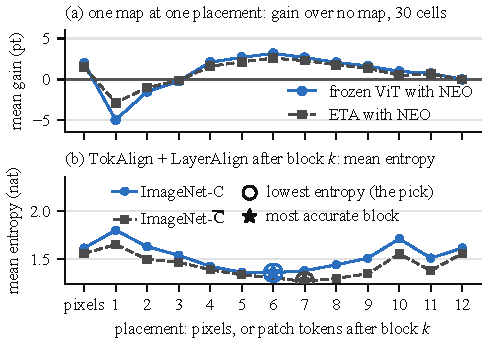
\includegraphics[width=3.25in]{../figures/depth_curve.pdf}
\caption{\textbf{Where to align a frozen ViT-B/16, and how the entropy finds it} (30 dev cells, \cref{sec:results}). (a)~The map at one placement at a time: mean gain in top-1 points over the same model without the map, frozen with \neo{} and ETA with \neo{}. (b)~\tok{} plus \layer{} after block $k$: mean prediction entropy on the unlabeled images. The lowest entropy (circle) falls on the most accurate block (star) on both benchmarks.}
\label{fig:depth}
\end{figure}

\section{Related Work}
\label{sec:related}
\paragraph{Where to adapt.} Surgical fine-tuning, layer-wise auto-weighting, GALA and ZOTTA choose which layers a gradient updates \citep{surgical2023,layerwise2024,gala2025,zotta2026}, and Hi-Vec picks a classifier head per batch by a gradient norm \citep{hivec2026}. All need gradients, where ours sweeps the depth of a closed-form map that updates no parameter.

\paragraph{Gradient-free test-time adaptation.} Batch-normalization adaptation re-estimates the statistics of every normalization layer \citep{schneider2020,aqr2025,quar2026}. \neo{} re-centers the head input of a ViT \citep{neo2026}, and LinearTCA, CFA and CAFe align the output or penultimate features \citep{tca2025,cfa2022,cafe2023}. T3A and LAME adjust the classifier without gradients \citep{t3a2021,lame2022}, PEA aligns the covariance after every block in two passes \citep{pea2026}, ActMAD matches activation statistics at several layers by gradient \citep{actmad2023}, and FOA searches prompt tokens with an evolution strategy \citep{foa2024}. All fix their placements by convention.

\paragraph{Gradient-based TTA, cascades and test-time ensembles.} Tent, ETA and SAR update normalization parameters by backpropagating prediction entropy \citep{tent2021,eata2022,sar2023}. Early exits stop easy inputs early \citep{branchynet2016,msdnet2018}, adaptive ViTs drop tokens or layers \citep{dynamicvit2021,adavit2022,avit2022}, cascades pass unsure inputs on \citep{committees2022} and test-time ensembles average views \citep{ttaagg2021}. Their members are exits, models or views. Ours differ only in where one map acts.

\section{Method}
\label{sec:method}
\paragraph{Task.} A frozen ViT classifies a stream of unlabeled test batches of 64 images, each cut into 196 patches. We write $x\in\mathbb{R}^{768}$ for a normalized $16{\times}16{\times}3$ pixel patch, $t_k\in\mathbb{R}^{d}$ for a patch token after block $k$ and $h\in\mathbb{R}^{d}$ for the head input ($d{=}768$ for ViT-B/16, 384 for ViT-S/16). One forward pass over $N_s{=}3{,}000$ unlabeled clean validation images gives the source statistics: the mean and covariance of the pixel patches $(\mu_s,\Sigma_s)$ and of the patch tokens after every block $(\mu^k_s,\Sigma^k_s)$. Nothing below uses a label or a gradient (\cref{fig:overview}, \cref{fig:framework}).

\begin{figure*}[t]
\centering
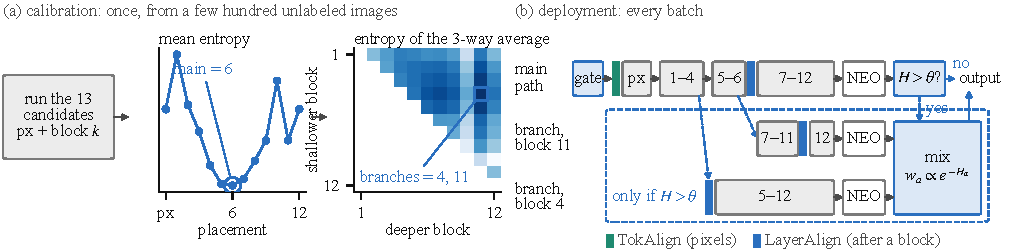
\includegraphics[width=6.75in]{../figures/overview.pdf}
\caption{\textbf{The calibrated cascade.} (a)~Calibration, once, from unlabeled images: the 13 placements are run. The placement with the lowest mean prediction entropy gives the main block, and the pair of other blocks whose confidence-weighted average with the main path has the lowest entropy on the unsure images gives the two branches (ImageNet-C dev images). (b)~Deployment, every batch: every image runs the main path, an unsure image ($H>\theta$) also runs the dashed box, and the three predictions are averaged by confidence.}
\label{fig:overview}
\end{figure*}

\subsection{One map, placed anywhere}
\label{sec:map}
We use one closed-form map, the whitening and recoloring of CORAL \citep{coral2016} with a source prior, at a chosen \emph{placement}, the pixel patches or the patch tokens after block $k$. There the map keeps the running mean $m_t$ and covariance $\Sigma_t$ of the vectors it sees. The estimate is shrunk toward the source statistics $(\mu_s,\Sigma_s)$ of the same placement:
\begin{equation}
\hat\Sigma = (1-\lambda)\,\frac{n\,\Sigma_t + n_0\,\Sigma_s}{n+n_0} + \lambda\,\Sigma_s ,
\label{eq:shrink}
\end{equation}
where $n$ is the number of vectors seen, $n_0$ is four images' worth of vectors and $\lambda{=}0.1$. Every vector is then mapped by
\begin{equation}
x' = \Sigma_s^{1/2}\,\hat\Sigma^{-1/2}\,(x - m_t) + \mu_s .
\label{eq:map}
\end{equation}
At the pixels we call this map \emph{\tok{}}. After block $k$ it acts on the 196 patch tokens, not the class token, and we call it \emph{\layer{}}. Each map costs one $d{\times}d$ multiply per token.

\subsection{The main path and its gate}
\label{sec:stack}
The \emph{main path} applies \cref{eq:map} at the pixels and after the \emph{main block} $b$ that \cref{sec:calib} picks (6 on ImageNet-C). \neo{} follows at the head, subtracting the running mean $\bar h_t$ of $h$ \citep{neo2026}. One gate keeps both maps off on batches that have not shifted, so that clean batches run as \neo{} alone: it opens when the DCT power spectrum of the pixel patches or their mean departs from the source's by more than a threshold set on clean images (\cref{alg:stack}, \cref{app:settings}). The same two scores on a placement's tokens, as $z$-scores against clean batches, measure its \emph{drift}.

\subsection{Extra branches for the unsure images}
\label{sec:exit}
The cascade (\cref{fig:overview}) spends extra computation only on the images the main path is unsure of, where a second prediction can still change the answer (random images, same share: about two fifths as much, \cref{tab:exit}). Every image runs the main path, and one whose prediction entropy $H$ is at most $\theta$ is output as it is. One with $H>\theta$ also runs two \emph{extra branches}, which place \layer{} after two other blocks $a_1<a_2$ instead of the main block, each with its own statistics and \neo{} mean (a branch above the main block runs on tokens its map did not touch). The predictions $p_a$ of the main path and the two branches are averaged per image with weights $w_a\propto\exp(-H_a)$, where $H_a$ is the entropy of $p_a$, so the surer prediction counts more.

\subsection{Calibration: the three blocks and the threshold, without labels}
\label{sec:calib}
The three blocks and $\theta$ are chosen once before deployment, from unlabeled images of the target distribution, by the same entropy. This assumes the test images come from the calibration's shifts (\cref{app:limits}). The 13 placements, \tok{} alone and \tok{} plus \layer{} after block $k$, run on those images. The \emph{main block} is the placement with the lowest mean entropy (\tok{} alone is a candidate here). The two \emph{branch blocks} are the pair of other blocks, out of every pair of the other eleven, whose confidence-weighted average with the main path has the lowest mean entropy on the images the main path is unsure of. The threshold $\theta$ is the 0.65 quantile of the main path's entropy on those images, so about a third run the extra branches. The ViT-B/16 runs on both corruption benchmarks and ViT-S/16 on ImageNet-C use 1.5\,nat, fixed before the rule existed, which the quantile was set to reproduce (the gain is flat in it, \cref{app:calib}). On ImageNet-C the calibration gives main block \pn{rl.pick.inc.trunk} and extra branches after blocks \pn{rl.pick.inc.lo} and \pn{rl.pick.inc.hi} (\cref{fig:overview}a).

\section{Results}
\label{sec:results}
\paragraph{Setup.} ImageNet-C \citep{imagenetc2019} has 15 corruptions at severities 3 and 5. A \emph{cell} is one corruption at one severity, 2{,}000 images, so there are 30 cells plus the clean cell. ImageNet-$\overline{\text{C}}$ \citep{mintun2021} adds ten corruptions unlike ImageNet-C's (20 cells), and ImageNet-R \citep{imagenetr2021} and ImageNet-Sketch \citep{sketch2019} are natural shifts, cut into 2{,}000-image cells (\cref{app:splits}). Models: timm AugReg ViT-B/16 and ViT-S/16 \citep{augreg2022,timm} and DeiT-B/16 \citep{deit2021} (DeiT-S/16 in the supplement), 224\,px, batch 64, official \neo{}, ETA and SAR code, one run per number. Every choice was made on the \emph{dev} images. Every \emph{held-out} result is on disjoint images that no choice touched, run once (95\% bootstrap intervals over images and over cells in \cref{app:ci}). We report \textbf{top-1 accuracy} averaged over the cells, \textbf{gains} in points, the \textbf{clean} cell, and the share of \textbf{unsure} images that run the extra branches.

\paragraph{Where to align: mid-depth gains most, and two maps beat one.} \Cref{fig:depth}a places the map at each of the 13 placements of ViT-B/16 in turn. With \neo{}, \tok{} gains \pn{ts.sw.frozen.pixel} points, blocks 5 to 8 gain \pn{ts.sw.frozen.mid.lo} to \pn{ts.sw.frozen.mid.hi} and blocks 1 to 3 lose. Only \tok{} helps on noise (\cref{fig:depthfam}), so the two maps correct different shifts, and the main path (pixels $+$ block 6) gains \pn{ts.d.gain.twosite} points, above the oracle over the 13 single placements (\cref{app:percell}). Held out, the main path gains \pn{ts.hb.gain.twosite} over \neo{} and adds to ETA and SAR (\cref{app:base}).

\paragraph{Which block: confidence, not drift.} For \pn{ts.dr.pixelmax.n} of the 15 corruptions the drift is largest at the pixels (\cref{fig:drift}), and rules that pick the block from the drift fall below the main path (\cref{app:drift}). The mean prediction entropy of the 13 placements instead ranks them as their accuracy does (\cref{fig:depth}b, Spearman \pn{sc.inc.lf.trunk.rho}, \pn{rc.vitb_inc.rho4} without blocks 1 to 3) and picks the most accurate block, as the objective of MECA predicts \citep{meca2018}.

\begin{table}[t]
\caption{\textbf{The calibrated cascade on held-out images} (ViT-B/16, the fourth held-out set, 2{,}000 fresh images per cell, every row run once, no gradients). Top-1 \% on the 30 ImageNet-C cells (C), the 20 ImageNet-$\overline{\text{C}}$ cells and the clean cell. Unsure: images whose main-path entropy exceeds $\theta$ and run the extra branches, on C (\pn{rl.h.cbar.b4b11.routed}\% on $\overline{\text{C}}$). Time: per batch relative to \neo{}, on six dev cells. Bold: the best in the column.}
\label{tab:exit}
\vskip 0.05in
\centering
\footnotesize
\setlength{\tabcolsep}{1.1pt}
\begin{tabular}{l rrr r r}
\toprule
 & \multicolumn{3}{c}{top-1 \%} & & \\
\cmidrule(lr){2-4}
 & C & $\overline{\text{C}}$ & clean & unsure & time \\
\midrule
\neo{} & \pn{ex.h.inc.neo} & \pn{ex.h.cb.neo} & \pn{ex.h.clean.neo} & 0\% & \pn{rl.cost.neo.x} \\
\quad $+$ \tok{} & \pn{ex.h.inc.tok} & \pn{ex.h.cb.tok} & \pn{ex.h.clean.tok} & 0\% & \pn{rl.cost.tok.x} \\
\quad $+$ \layer{} at 6 (main path) & \pn{ex.h.inc.pairg} & \pn{ex.h.cb.pairg} & \pn{ex.h.clean.pairg} & 0\% & \pn{rl.cost.pair.x} \\
\textbf{\quad $+$ branches 4, 11 (cascade)} & \textbf{\pn{rl.h.inc.b4b11}} & \textbf{\pn{rl.h.cbar.b4b11}} & \pn{rl.h.inc.b4b11.clean} & \pn{rl.h.inc.b4b11.routed}\% & \pn{rl.cost.b4b11.x} \\
\qquad branch 4 only & \pn{rl.h.inc.b4} & \pn{rl.h.cbar.b4} & \pn{rl.h.inc.b4.clean} & \pn{rl.h.inc.b4.routed}\% & \pn{rl.cost.b4.x} \\
\qquad branch 11 only & \pn{rl.h.inc.b11} & \pn{rl.h.cbar.b11} & \pn{rl.h.inc.b11.clean} & \pn{rl.h.inc.b11.routed}\% & \pn{rl.cost.b11.x} \\
\qquad random images, same share & \pn{rl.ctl.inc.random} & \pn{rl.ctl.cbar.random} & \pn{rl.ctl.inc.random.cleanabs} & \pn{rl.ctl.inc.random.routed}\% & \pn{rl.cost.random.x} \\
\bottomrule
\end{tabular}
\end{table}

\paragraph{The calibrated cascade on held-out images.} \Cref{tab:exit} reads from \neo{} down: \tok{} adds \pn{ex.h.inc.gainneo.tok} points on ImageNet-C, \layer{} after the calibrated block 6 brings the main path to \pn{ex.h.inc.gainneo.pairg} over \neo{}, and the calibrated branches add \pn{rl.h.inc.b4b11.gain} more (\pn{rl.h.inc.b4b11.gainneo} over \neo{}), with clean accuracy unchanged. On ImageNet-$\overline{\text{C}}$, which took no part in the calibration, they add \pn{rl.h.cbar.b4b11.gain} (\pn{rl.h.cbar.b4b11.gainneo} over \neo{}). Random images gain \pn{rl.ctl.inc.random.gain} and \pn{rl.ctl.cbar.random.gain}, three views of the main path \pn{rl.ctl.inc.views.gain} and \pn{rl.ctl.cbar.views.gain}, so averaging gives most of the branch gain, the placements the rest (\cref{app:controls}). On the dev cells, where our settings were chosen, the cascade is above ETA and SAR with \neo{} and above PEA and FOA, which stay below their published accuracy (\cref{tab:others}, \cref{app:settings}), and on a continual stream of 15 held-out cells it stays \pn{rl.st.cont.cascade.vs.etaneo} points above ETA with \neo{} (\cref{app:sets}).

\paragraph{A few hundred unlabeled images calibrate the cascade.} From \pn{rl.ss.small.n} images per cell the calibration picks other blocks whose cascade gains \pn{rl.h.inc.small.gainfull} and \pn{rl.h.cbar.small.gainfull} over the full-sample main path held out, against \pn{rl.h.inc.b4b11.gainfull} and \pn{rl.h.cbar.own.gainfull} for the full-sample picks, and one calibration per shift from \pn{rl.ss.inc.k3.n} images gains \pn{rl.fs.inc.k3.vsfullbase} and \pn{rl.fs.cbar.k3.vsfullbase} over the full-sample main path (main block \pn{rl.fs.inc.k3.vsfullbase.base} and \pn{rl.fs.cbar.k3.vsfullbase.base} of it, branches \pn{rl.fs.inc.k3.gain} and \pn{rl.fs.cbar.k3.gain}, \cref{tab:calibsize}).

\begin{table}[t]
\caption{\textbf{How many unlabeled images the calibration needs} (ViT-B/16, gain of the cascade over the full-sample main path of the benchmark, block 6 on C and block 7 on $\overline{\text{C}}$, in top-1 points). Dev pred.: blocks chosen from the first $n$ images of the saved dev predictions and scored on all of them ($\overline{\text{C}}$ gains moved to the block-7 reference, \pn{rl.ss.cbar.ref.shift}). Held-out: those blocks run once on fresh images (on C the 320 and 192 picks coincide, one run). Per benchmark: the first $n$ images of every cell. Per shift: the first batches of that shift.}
\label{tab:calibsize}
\vskip 0.05in
\centering
\footnotesize
\setlength{\tabcolsep}{1.5pt}
\begin{tabular}{l rr rr}
\toprule
 & \multicolumn{2}{c}{C} & \multicolumn{2}{c}{$\overline{\text{C}}$} \\
\cmidrule(lr){2-3}\cmidrule(lr){4-5}
calibration images & dev pred. & held-out & dev pred. & held-out \\
\midrule
\multicolumn{5}{l}{\textit{one calibration per benchmark}} \\
2,000 per cell (all) & \pn{rl.ss.inc.full.gain} & \pn{rl.h.inc.b4b11.gainfull} & \pn{rl.ss.cbar.full.gain} & \pn{rl.h.cbar.own.gainfull} \\
320 per cell & \pn{rl.ss.inc.n320.gain} & \pn{rl.h.inc.small.gainfull} & \pn{rl.ss.cbar.n320.gain} & \pn{rl.h.cbar.small.gainfull} \\
192 per cell & \pn{rl.ss.inc.n192.gain} & \pn{rl.h.inc.small.gainfull} & \pn{rl.ss.cbar.n192.gain} & \pn{rl.ss.cbar.p192.held.gain} \\
\multicolumn{5}{l}{\textit{one calibration per shift}} \\
640 per shift (10 batches) & \pn{rl.ss.inc.k10.gain} & \pn{rl.fs.inc.k10.vsfullbase} & \pn{rl.ss.cbar.k10.gain} & \pn{rl.fs.cbar.k10.vsfullbase} \\
192 per shift (3 batches) & \pn{rl.ss.inc.k3.gain} & \pn{rl.fs.inc.k3.vsfullbase} & \pn{rl.ss.cbar.k3.gain} & \pn{rl.fs.cbar.k3.vsfullbase} \\
64 per shift (1 batch) & \pn{rl.ss.inc.k1.gain} & \pn{rl.fs.inc.k1.vsfullbase} & \pn{rl.ss.cbar.k1.gain} & \pn{rl.fs.cbar.k1.vsfullbase} \\
\bottomrule
\end{tabular}
\end{table}

\begin{table}[!t]
\caption{\textbf{Across models and shifts, with the calibration repeated for each pair} (held-out cells, gains in top-1 points over \neo{}, intervals in \cref{tab:ci}. ViT-B/16 and ViT-S/16 on C use the third held-out set, the other corruption rows the fourth, Sketch its three held-out cells. $\theta$: 1.5\,nat for ViT-B/16 on the corruptions and ViT-S/16 on C, else the 0.65 quantile). Pick: main block / branch blocks. $\rho$: Spearman correlation of mean entropy and accuracy over the 13 placements on dev images. Ours, no gradients: the main path and the cascade. ETA with \neo{}, gradient-based: alone, with our main path inside, with the cascade inside. S: Sketch (ImageNet-R in \cref{tab:natural}). Bold: the best of the row among ours, underlined among the ETA columns.}
\label{tab:across}
\vskip 0.05in
\centering
\scriptsize
\setlength{\tabcolsep}{1.4pt}
\begin{tabular}{ll l r rr rrr}
\toprule
& & & & \multicolumn{2}{c}{ours} & \multicolumn{3}{c}{ETA with \neo{}} \\
\cmidrule(lr){5-6}\cmidrule(lr){7-9}
model & shift & pick & $\rho$ & main & cascade & alone & $+$main & $+$cascade \\
\midrule
ViT-B & C & \pn{ax.vitb_inc.pick} & \pn{ax.vitb_inc.rho} & \pn{ax.vitb_inc.base} & \textbf{\pn{ax.vitb_inc.stack}} & \pn{ax.vitb_inc.eta} & \pn{ax.vitb_inc.etaours} & \underline{\pn{ax.vitb_inc.etastack}} \\
ViT-S & C & \pn{ax.vits_inc.pick} & \pn{ax.vits_inc.rho} & \pn{ax.vits_inc.base} & \textbf{\pn{ax.vits_inc.stack}} & \pn{ax.vits_inc.eta} & \pn{ax.vits_inc.etaours} & \underline{\pn{ax.vits_inc.etastack}} \\
DeiT-B & C & \pn{ax.deitb_inc.pick} & \pn{ax.deitb_inc.rho} & \pn{ax.deitb_inc.base} & \textbf{\pn{ax.deitb_inc.stack}} & \pn{ax.deitb_inc.eta} & \pn{ax.deitb_inc.etaours} & \underline{\pn{ax.deitb_inc.etastack}} \\
\midrule
ViT-B & $\overline{\text{C}}$ & \pn{ax.vitb_cbar.pick} & \pn{ax.vitb_cbar.rho} & \pn{ax.vitb_cbar.base} & \textbf{\pn{ax.vitb_cbar.stack}} & \pn{ax.vitb_cbar.eta} & \pn{ax.vitb_cbar.etaours} & \underline{\pn{ax.vitb_cbar.etastack}} \\
ViT-S & $\overline{\text{C}}$ & \pn{ax.vits_cbar.pick} & \pn{ax.vits_cbar.rho} & \pn{ax.vits_cbar.base} & \textbf{\pn{ax.vits_cbar.stack}} & \pn{ax.vits_cbar.eta} & \pn{ax.vits_cbar.etaours} & \underline{\pn{ax.vits_cbar.etastack}} \\
DeiT-B & $\overline{\text{C}}$ & \pn{ax.deitb_cbar.pick} & \pn{ax.deitb_cbar.rho} & \pn{ax.deitb_cbar.base} & \textbf{\pn{ax.deitb_cbar.stack}} & \pn{ax.deitb_cbar.eta} & \pn{ax.deitb_cbar.etaours} & \underline{\pn{ax.deitb_cbar.etastack}} \\
\midrule
ViT-B & S & \pn{ax.vitb_sketch.pick} & \pn{ax.vitb_sketch.rho} & \pn{ax.vitb_sketch.base} & \textbf{\pn{ax.vitb_sketch.stack}} & \pn{ax.vitb_sketch.eta} & \pn{ax.vitb_sketch.etaours} & \underline{\pn{ax.vitb_sketch.etastack}} \\
ViT-S & S & \pn{ax.vits_sketch.pick} & \pn{ax.vits_sketch.rho} & \pn{ax.vits_sketch.base} & \textbf{\pn{ax.vits_sketch.stack}} & \underline{\pn{ax.vits_sketch.eta}} & \pn{ax.vits_sketch.etaours} & \pn{ax.vits_sketch.etastack} \\
DeiT-B & S & \pn{ax.deitb_sketch.pick} & \pn{ax.deitb_sketch.rho} & \pn{ax.deitb_sketch.base} & \textbf{\pn{ax.deitb_sketch.stack}} & \pn{ax.deitb_sketch.eta} & \pn{ax.deitb_sketch.etaours} & \underline{\pn{ax.deitb_sketch.etastack}} \\
\bottomrule
\end{tabular}
\end{table}

\paragraph{Across models and shifts.} \Cref{tab:across} repeats the procedure for three backbones and three shifts. On the six corruption pairs the entropy tracks the accuracy ($\rho$ \pn{ax.deitb_cbar.rho} to \pn{ax.deitb_inc.rho}, \cref{fig:signalgrid}) and the gradient-free cascade beats ETA with \neo{} in all six. The extra branches add \pn{ax.vitb_cbar.stack.vsbase} to \pn{rl.vs.both.gain} where neither branch block is next to the main block, but only \pn{ax.deitb_inc.stack.vsbase} to \pn{ax.vits_cbar.stack.vsbase} where one is (\cref{app:why}). On Sketch, as on ImageNet-R (\cref{tab:natural}), the backbone decides: the AugReg ViTs gain at most \pn{ca.vits_sketch.best.gainneo} from their best block and ETA wins, while DeiT-B/16 gains \pn{ax.deitb_sketch.stack} and \pn{ax.deitb_r.stack} over \neo{}, above ETA.

\section{Conclusion}
\label{sec:conclusion}
On corruption shifts the model's confidence, not the drift, says where a frozen ViT should align. A few hundred unlabeled images calibrate the three blocks, the same entropy decides per image whether the branches run, and the cascade gains \pn{rl.h.inc.b4b11.gainneo} points over \neo{} held out. It cannot notice a shift outside its calibration or tell where no block helps (\cref{app:limits}).

\bibliography{refs}
\bibliographystyle{icml2026}

\clearpage
\appendix
\onecolumn
\renewcommand{\topfraction}{0.95}\renewcommand{\bottomfraction}{0.9}\renewcommand{\textfraction}{0.05}\renewcommand{\floatpagefraction}{0.85}
\setlength{\textfloatsep}{10pt plus 2pt minus 4pt}\setlength{\floatsep}{8pt plus 2pt minus 2pt}\setlength{\intextsep}{8pt plus 2pt minus 2pt}
\makeatletter\setlength{\@fptop}{0pt}\setlength{\@fpsep}{8pt plus 2pt}\makeatother  % supplement float pages start at the top
\renewcommand{\thesection}{\Alph{section}}
\renewcommand{\thetable}{S\arabic{table}}
\renewcommand{\thefigure}{S\arabic{figure}}
\renewcommand{\thealgorithm}{S\arabic{algorithm}}
\setcounter{table}{0}
\setcounter{figure}{0}

\begin{center}{\Large\bfseries Supplementary Material}\end{center}

This supplement holds the evidence behind the three contributions of the report. \Cref{app:overview} states the algorithm on one real batch and \cref{app:splits} the data and the one procedure every model-shift pair goes through. \Cref{app:where} is about the entropy as the criterion (contribution 1): the 13 placements per corruption, the entropy against the accuracy across models and shifts, and why the drift does not do the same. \Cref{app:calib} is about the calibration (contribution 2): what it picks, why these two blocks, how many images it needs. \Cref{app:exit} gives the calibrated cascade on held-out images in full: per corruption, over image sets and in time, its ablations and controls, the main path inside ETA and SAR, and the comparison with other test-time adaptation methods. \Cref{app:limits} states the limitations, \cref{app:negatives} lists what did not work, including where the entropy fails (contribution 3), and \cref{app:settings} gives the settings and licenses.

\section{One Batch Through the Cascade}
\label{app:overview}
\Cref{fig:framework} follows one batch of the dev split through the calibrated cascade of \cref{sec:stack,sec:exit}, which \cref{alg:stack} states step by step for the calibrated blocks $b$, $a_1$ and $a_2$. The pixel part is recomputed from the cached images with the repository's code and the running statistics of the run up to that batch, so the map shown is the map the run applied. The token values inside the network are not recomputed, so the network rows are schematic. The inset is real: it is the entropy of the main path's predictions on the 2{,}000 dev images of the cell, from the saved logits, and the share above the threshold equals the share of images the run sent to the extra branches.

\begin{algorithm}[!ht]
\caption{One batch of the calibrated cascade (blocks chosen by the calibration: main $b$ and the branches $a_1<a_2$, which are 6, 4 and 11 on ImageNet-C and ViT-B/16)}
\label{alg:stack}
\small
\begin{algorithmic}[1]
\REQUIRE a batch $X$ of 64 images, the source statistics, the running statistics, the calibrated blocks $b$, $a_1$, $a_2$ and the threshold $\theta$
\STATE $P \leftarrow \mathrm{unfold}(X)$ \hfill\COMMENT{the 196 pixel patches of every image}
\STATE $g \leftarrow g_{\text{spec}}(P) > 0.4$ \textbf{or} $g_{\text{mean}}(P) > 0.3$ \hfill\COMMENT{the gate, read from the patches before the model runs}
\STATE update the running mean and covariance $(m_t, \Sigma_t)$ with $P$
\IF{$g$}
\STATE $\hat\Sigma \leftarrow$ \cref{eq:shrink} and $X \leftarrow \mathrm{fold}\big(\Sigma_s^{1/2}\hat\Sigma^{-1/2}(P-m_t)+\mu_s\big)$ \hfill\COMMENT{\tok{}}
\ENDIF
\STATE $T \leftarrow \mathrm{blocks}_{1..b}(\mathrm{embed}(X))$, keeping the tokens $T_a$ after each branch block $a<b$ \hfill\COMMENT{the unmapped tokens after block $b$}
\IF{$g$}
\STATE patch tokens of $T \leftarrow (\Sigma^b_s)^{1/2}(\hat\Sigma^b)^{-1/2}(t-m^b_t)+\mu^b_s$, class token unchanged \hfill\COMMENT{\layer{} after the main block}
\ENDIF
\STATE $p_b \leftarrow \mathrm{softmax}\big(\mathrm{head}(\mathrm{norm}(\mathrm{blocks}_{b+1..12}(T))_{\text{cls}}-\bar h_t)\big)$ \hfill\COMMENT{the main path, \neo{} at the head}
\IF{\textbf{not} $g$}
\STATE \textbf{return} $p_b$ \hfill\COMMENT{no shift: the batch runs as \neo{} alone}
\ENDIF
\STATE $S \leftarrow \{i : H(p_{b,i}) > \theta\}$ \hfill\COMMENT{the unsure images}
\FOR{each branch block $a \in \{a_1, a_2\}$}
\STATE $U \leftarrow T_a[S]$ if $a<b$, else $\mathrm{blocks}_{b+1..a}(T[S])$ \hfill\COMMENT{the unsure images' tokens after block $a$, mapped only at the pixels}
\STATE $p_a \leftarrow$ \layer{} after block $a$ on $U$, then $\mathrm{blocks}_{a+1..12}$, its own \neo{} mean and the head \hfill\COMMENT{the branch}
\ENDFOR
\STATE \textbf{return} $p_b$ outside $S$, and $\sum_a w_a p_a$ with $w_a \propto e^{-H(p_a)}$ over $a \in \{b, a_1, a_2\}$ inside $S$ \hfill\COMMENT{confidence-weighted average}
\end{algorithmic}
\end{algorithm}

\section{Data, Models and the Procedure}
\label{app:splits}
\begin{figure}[t]
\centering
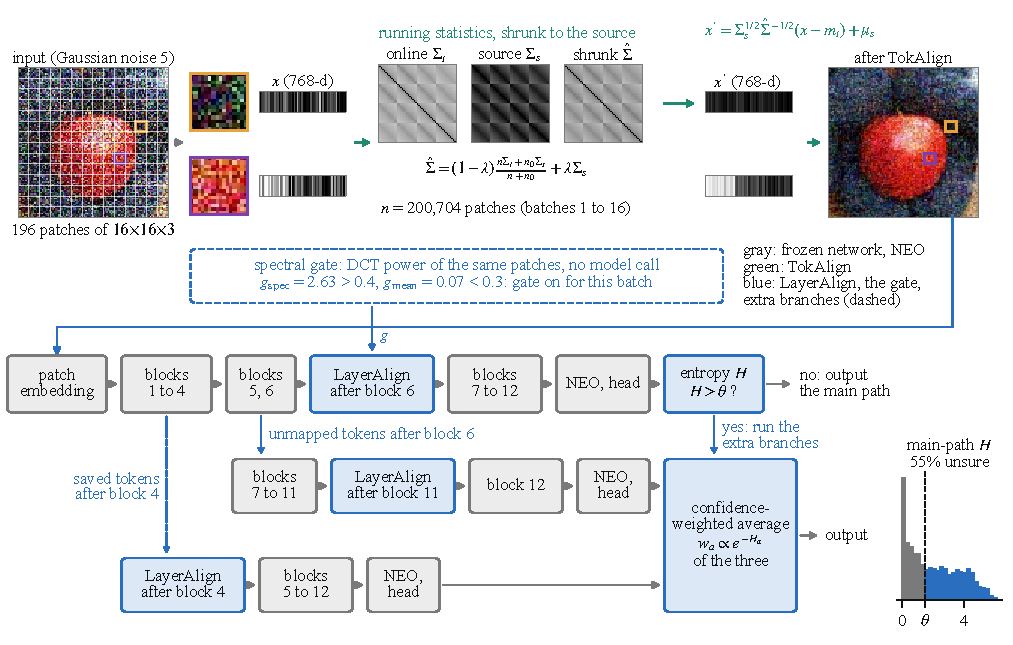
\includegraphics[width=6.75in]{../figures/framework.pdf}
\caption{\textbf{One batch through the calibrated cascade.} Top: the input image (Gaussian noise, severity 5) is cut into 196 patches, and two of them (orange: the flattest patch of the clean image, purple: the most textured) are shown as 768-d vectors. The running patch covariance $\Sigma_t$ of the cell is shrunk toward the source covariance $\Sigma_s$ (\cref{eq:shrink}, the first 64 of the 768 coordinates, one grey scale), and the map of \cref{eq:map} sends every patch to $x'$, folded back into the image on the right. The dashed box is the gate, read from the same patches without a model call. Middle: the main path, \tok{} and \layer{} after the main block (block 6, the block the calibration picks on ImageNet-C), followed by \neo{} and the classifier. Bottom: an image whose main-path entropy $H$ exceeds $\theta{=}1.5$\,nat also runs the two extra branches, \layer{} after block 4 on the saved tokens and \layer{} after block 11 on the unmapped tokens after the main block, both chosen by the same calibration, each with its own statistics and \neo{} mean. The three predictions are averaged with weights $\propto e^{-H_a}$. Right: the main-path entropy of the 2{,}000 images of this cell, with the unsure images in blue. Grey boxes are the frozen network or \neo{}. Green marks \tok{} and blue \layer{}, the gate and the extra branches, as in \cref{fig:overview}. When the gate is off, only \neo{} acts.}
\label{fig:framework}
\end{figure}

\subsection{Splits}
All ImageNet splits are fixed permutations of the 50{,}000 validation indices. The 2{,}000 \emph{dev} images per cell carry every choice of this project: $\lambda{=}0.1$, the priors, the EMA rates, the gate thresholds 0.4 and 0.3, the ETA configuration, and the calibration of every model-shift pair. The source statistics come from 3{,}000 clean images of a disjoint split, whose labels are never read. Held-out sets are disjoint 2{,}000-image sets per cell, untouched by any run before their own held-out run and run once. Each table states which set it uses.

ImageNet-$\overline{\text{C}}$ \citep{mintun2021} uses the same index splits and source statistics, with nothing re-tuned. ImageNet-R \citep{imagenetr2021} and ImageNet-Sketch \citep{sketch2019} are shuffled once and cut into cells of 2{,}000 images, three dev and three held-out cells each. Their images go through the clean transform of the model, and ImageNet-R logits are restricted to its 200 classes. The clean cell is the ImageNet validation cell of the split.

\subsection{One procedure per model-shift pair}
Every pair of \cref{tab:across} goes through the same five steps, and no step reads a label.
\begin{enumerate}
\setlength{\itemsep}{1pt}\setlength{\topsep}{2pt}\setlength{\parsep}{0pt}
\item One forward pass over the source images gives the source statistics of every placement.
\item The 13 placements, \tok{} plus \layer{} after each of the 12 blocks, and \tok{} alone, run on the dev cells with \neo{} at the head, together with \neo{} alone.
\item The calibration of \cref{sec:calib} reads the saved predictions of step 2 and returns the main block, the two branch blocks and $\theta$.
\item The held-out run: \neo{}, \tok{}, the main path and the calibrated cascade with its two single-branch versions, on the held-out cells, once.
\item The gradient-based comparison on the same held-out cells: ETA with \neo{}, with the main path's maps inside it, and with the whole cascade inside it.
\end{enumerate}
Labels enter only in scoring. Every block number in this report is an output of step 3: on ImageNet-C and ViT-B/16 the calibration returns main block 6 and extra branches after blocks 4 and 11, so the ImageNet-C tables below write 6 for the main block and 4, 11 for the branches. The ViT-B/16 runs and the ViT-S/16 run on ImageNet-C use $\theta{=}1.5$\,nat, fixed before the cascade's held-out run. The 0.65 quantile rule that every later pair uses gives \pn{rl.ss.inc.theta65}\,nat on the same ViT-B/16 images and \pn{rl.vs.theta65}\,nat on ViT-S/16, where 1.5\,nat sends \pn{rl.vs.both.routed}\% of the held-out images to the branches. Every gain in this report is the difference of two unrounded accuracies, so it can differ by 0.01 from the difference of the printed values. A labelled search over pairs of branch blocks on the dev cells, run with the spectral gate before the calibration existed, chose blocks 5 and 9. It appears in the tables as a comparison only. The four ImageNet-C held-out sets were opened in order: the first for \tok{} on ViT-B/16, the second for \tok{} on ViT-S/16, the third for the main path of both backbones, inside ETA and SAR as well, and the fourth for the calibrated cascade and its controls. No setting was changed after a set was opened, and the cascade's runs on the first three sets (\cref{tab:rulesl}) came after its run on the fourth.

\subsection{Models}
ViT-B/16 and ViT-S/16 are the timm AugReg checkpoints \citep{augreg2022,timm} (0.5 normalization, resize 248, center crop 224). DeiT-B/16 and DeiT-S/16 are the original DeiT checkpoints \citep{deit2021} (ImageNet mean and standard deviation, resize 256, center crop 224). DeiT-S/16 appears in the supplement only (\cref{fig:signalgrid}, \cref{tab:natural}). All runs are FP32 at batch 64 on one GPU, with TF32 disabled so that the eigendecompositions reproduce exactly. Every number is one run per 2{,}000-image cell.

\section{The Entropy Tracks the Accuracy of a Placement}
\label{app:where}
\subsection{The 13 placements per corruption}
\Cref{fig:depthfam} splits the depth sweep of \cref{fig:depth}a by corruption family: noise is the only family that gains from \tok{} alone, and blur, weather and digital shifts gain most from a map at mid-depth, so the pixels and mid-depth correct different shifts and the main path takes both. On ImageNet-C and ViT-B/16 the calibration returns main block 6 (\cref{app:calib}). On held-out images the main path with that block is at least as good as the better of its two maps alone on \pn{ts.fam.twosite.wins} of the 15 corruptions.

\begin{figure}[!ht]
\centering
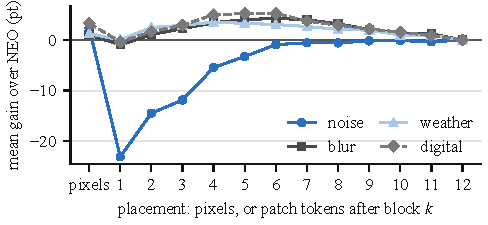
\includegraphics[width=3.25in]{../figures/depth_family.pdf}
\caption{\textbf{The depth sweep by corruption family} (frozen ViT-B/16 with \neo{}, 30 dev cells, mean gain over \neo{} per family of the map at one placement at a time). Noise is the only family that gains from \tok{} alone. Blur, weather and digital gain most at mid-depth.}
\label{fig:depthfam}
\end{figure}

\subsection{Entropy against accuracy across models and shifts}
\label{app:signal}
\Cref{fig:signalgrid} draws, for every model-shift pair, the accuracy of the 13 placements on the dev images, which uses labels and serves only as the check, and their mean prediction entropy, which uses none. On the corruption shifts the two curves mirror each other: the entropy ranks the placements as their accuracy does (Spearman \pn{sc.inc.lf.trunk.rho} on ImageNet-C and \pn{sc.cb.lf.trunk.rho} on ImageNet-$\overline{\text{C}}$ for ViT-B/16, \pn{ax.vits_inc.rho} for ViT-S/16, \pn{ax.deitb_inc.rho} for DeiT-B/16, \pn{ax.deits_inc.rho} for DeiT-S/16), and the lowest entropy falls on the most accurate block on three of the four ImageNet-C pairs and \pn{rc.vits_inc.gap} points from it on ViT-S/16. On ImageNet-$\overline{\text{C}}$ it picks block 7 for ViT-B/16 and ViT-S/16 ($\rho$ \pn{ax.vitb_cbar.rho} and \pn{ax.vits_cbar.rho}, the most accurate block for ViT-B/16 and \pn{ca.vits_cbar.pick.gap} points from it for ViT-S/16) and block 6 for DeiT-B/16 ($\rho$ \pn{ax.deitb_cbar.rho}, \pn{ca.deitb_cbar.pick.gap} points from block 7), and block \pn{ca.deits_cbar.trunk} for DeiT-S/16 ($\rho$ \pn{ca.deits_cbar.rho}, \pn{ca.deits_cbar.pick.gap} points from block \pn{ca.deits_cbar.best}). The first three blocks are the least confident and the least accurate placements on every corruption pair, so the entropy also keeps the calibration away from the depths where the map hurts. They do not carry the correlation: over \tok{} alone and blocks 4 to 12 it is \pn{rc.corr.rho4.min} to \pn{rc.corr.rho4.max} on the eight corruption pairs, against \pn{rc.nat.rho4.min} to \pn{rc.nat.rho4.max} on the eight natural pairs (\cref{tab:ci}).

On the natural shifts the backbone decides (\cref{tab:natural}). On ImageNet-R \layer{} helps either AugReg ViT at no block: \tok{} alone is the most accurate placement and \layer{} at every block is below it, so the calibration can only pick the least harmful block, and it does not: it picks block \pn{ca.vitb_r.trunk} for ViT-B/16 ($\rho$ \pn{ca.vitb_r.rho}, \pn{ca.vitb_r.pick.gap} points below \tok{}) and block \pn{ca.vits_r.trunk} for ViT-S/16 ($\rho$ \pn{ca.vits_r.rho}, \pn{ca.vits_r.pick.gap}). On Sketch a late block helps: ViT-B/16 picks block \pn{ca.vitb_sketch.trunk}, the most accurate ($\rho$ \pn{ca.vitb_sketch.rho}), but ViT-S/16 picks block \pn{ca.vits_sketch.trunk} where block \pn{ca.vits_sketch.best} is best, \pn{ca.vits_sketch.pick.gap} points away. The aligned placements become more confident than accurate: \layer{} after a mid-depth block lowers the entropy of a rendition or a sketch without raising its accuracy, so the entropy, which only reads confidence, cannot tell, the failure of entropy that \citet{deyo2024} describe for gradient-based TTA. The entropy a pick saves against \tok{} alone does not flag these cases either: it is \pn{rc.nat.miss.saved}\,nat on the four natural pairs the calibration misses and \pn{rc.nat.hit.saved.min} to \pn{rc.nat.hit.saved.max} on the four it gets right (\pn{rc.corr.saved.min} to \pn{rc.corr.saved.max} on the corruption pairs, \cref{tab:ci}), so a margin on it was tried and separates nothing.

DeiT-B/16, pretrained on ImageNet-1k alone, has a block that helps on both shifts: the calibration picks block \pn{ca.deitb_r.trunk} on ImageNet-R, the most accurate ($\rho$ \pn{ca.deitb_r.rho}), and block \pn{ca.deitb_sketch.trunk} on Sketch, \pn{ca.deitb_sketch.pick.gap} points from the most accurate block ($\rho$ \pn{ca.deitb_sketch.rho}). Its cascade gains \pn{ca.deitb_r.h.stack.gainneo} and \pn{ca.deitb_sketch.h.stack.gainneo} over \neo{}, above ETA with \neo{} by \pn{ca.deitb_r.h.stack.vseta} and \pn{ca.deitb_sketch.h.stack.vseta}. DeiT-S/16 follows it on ImageNet-R: block \pn{ca.deits_r.trunk}, the most accurate ($\rho$ \pn{ca.deits_r.rho}), and a cascade \pn{ca.deits_r.h.stack.gainneo} over \neo{}, \pn{ca.deits_r.h.stack.vseta} above ETA with \neo{}. On Sketch it misses: the best block, \pn{ca.deits_sketch.best}, adds only \pn{ca.deits_sketch.best.gainneo} points to \neo{} on the dev images, the entropy barely ranks the placements ($\rho$ \pn{ca.deits_sketch.rho}) and picks block \pn{ca.deits_sketch.trunk}, \pn{ca.deits_sketch.pick.gap} points from the best. On held-out images its main path is \pn{ca.deits_sketch.h.base.gainneo} against \neo{} and the extra branches bring the cascade to \pn{ca.deits_sketch.h.stack.gainneo}.

The entropy reads the model's confidence correctly wherever some placement is both more confident and more accurate. Where a shift leaves nothing, or less than a point, for the map to correct, it cannot tell.

\begin{figure}[!t]
\centering
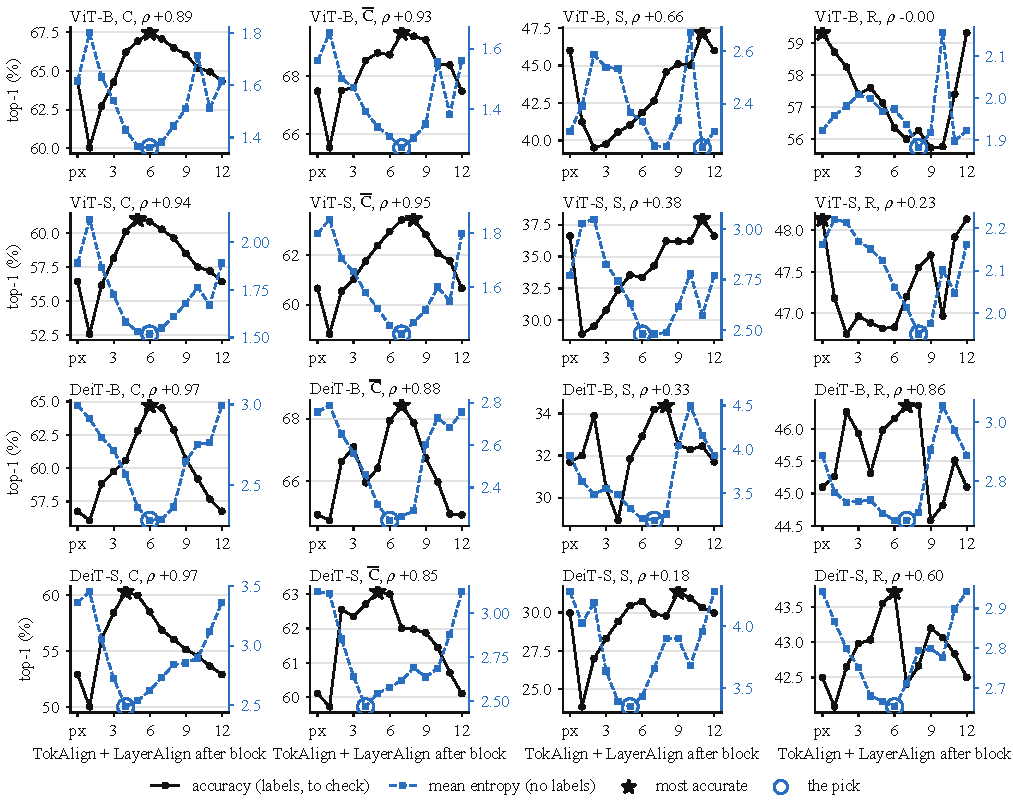
\includegraphics[width=6.75in]{../figures/signal_grid.pdf}
\caption{\textbf{Entropy against accuracy across models and shifts} (dev images, rows models, columns shifts, with C ImageNet-C, $\overline{\text{C}}$ ImageNet-$\overline{\text{C}}$, S Sketch and R ImageNet-R, and $x$ the 13 placements, \tok{} alone and \tok{} plus \layer{} after block $k$). Black: top-1 accuracy, which uses labels and serves only as the check. Blue: the mean prediction entropy of the placement on the same unlabeled images, which the calibration reads. The star marks the most accurate placement and the circle the placement the calibration picks, and $\rho$ is the Spearman correlation between entropy and accuracy over the 13 placements. On the corruption shifts (the C and $\overline{\text{C}}$ columns) the pick is the most accurate block or within half a point of it. On ImageNet-R it is for both DeiT models and on Sketch for DeiT-B/16 (within 0.2 points), but it misses in three of the four AugReg pairs and for DeiT-S/16 on Sketch, whose aligned placements are more confident than accurate.}
\label{fig:signalgrid}
\end{figure}

\begin{table}[!ht]
\caption{\textbf{The natural shifts in full} (ViT-B/16, ViT-S/16, DeiT-B/16 and DeiT-S/16, ImageNet-R over its 200 classes, held-out cells run once, gains in top-1 points). Calibration columns, read from the dev images: pick is the main block / the two branch blocks the calibration chose, best the most accurate block of the dev sweep (``none'' when \tok{} alone is the most accurate placement), $\rho$ as in \cref{fig:signalgrid}, gap the accuracy of the picked placement minus that of the most accurate placement, and $\theta$ the threshold in nat. Held-out columns: top-1 \% of \neo{}, \tok{}, the main path and the calibrated cascade, the gain of the cascade over the main path, and unsure, the share of images that run the extra branches. Then ETA with \neo{} (gradient-based), alone, with our main path inside it and with the whole cascade inside it. Bold: the best held-out accuracy of the row.}
\label{tab:natural}
\vskip 0.05in
\centering
\footnotesize
\setlength{\tabcolsep}{1.6pt}
\begin{tabular}{ll l l r r r rrrr r r rrr}
\toprule
 & & \multicolumn{5}{c}{calibration, dev images} & \multicolumn{6}{c}{held-out, top-1 \%} & \multicolumn{3}{c}{ETA with \neo{}, held-out} \\
\cmidrule(lr){3-7}\cmidrule(lr){8-13}\cmidrule(lr){14-16}
model & shift & pick & best & $\rho$ & gap & $\theta$ & \neo{} & \tok{} & main path & cascade & gain & unsure & alone & $+$ main path & $+$ cascade \\
\midrule
ViT-B & R & \pn{ca.vitb_r.trunk} / \pn{ca.vitb_r.lo}, \pn{ca.vitb_r.hi} & \pn{ca.vitb_r.best} & \pn{ca.vitb_r.rho} & \pn{ca.vitb_r.pick.gap} & \pn{ca.vitb_r.theta} & \pn{ca.vitb_r.h.neo} & \pn{ca.vitb_r.h.px} & \pn{ca.vitb_r.h.base} & \pn{ca.vitb_r.h.stack} & \pn{ca.vitb_r.h.stack.gain} & \pn{ca.vitb_r.h.stack.routed}\% & \pn{ca.vitb_r.eta.neo} & \pn{ca.vitb_r.eta.ours} & \textbf{\pn{ca.vitb_r.eta.stack}} \\
ViT-S & R & \pn{ca.vits_r.trunk} / \pn{ca.vits_r.lo}, \pn{ca.vits_r.hi} & \pn{ca.vits_r.best} & \pn{ca.vits_r.rho} & \pn{ca.vits_r.pick.gap} & \pn{ca.vits_r.theta} & \pn{ca.vits_r.h.neo} & \pn{ca.vits_r.h.px} & \pn{ca.vits_r.h.base} & \pn{ca.vits_r.h.stack} & \pn{ca.vits_r.h.stack.gain} & \pn{ca.vits_r.h.stack.routed}\% & \pn{ca.vits_r.eta.neo} & \pn{ca.vits_r.eta.ours} & \textbf{\pn{ca.vits_r.eta.stack}} \\
ViT-B & Sketch & \pn{ca.vitb_sketch.trunk} / \pn{ca.vitb_sketch.lo}, \pn{ca.vitb_sketch.hi} & \pn{ca.vitb_sketch.best} & \pn{ca.vitb_sketch.rho} & \pn{ca.vitb_sketch.pick.gap} & \pn{ca.vitb_sketch.theta} & \pn{ca.vitb_sketch.h.neo} & \pn{ca.vitb_sketch.h.px} & \pn{ca.vitb_sketch.h.base} & \pn{ca.vitb_sketch.h.stack} & \pn{ca.vitb_sketch.h.stack.gain} & \pn{ca.vitb_sketch.h.stack.routed}\% & \pn{ca.vitb_sketch.eta.neo} & \pn{ca.vitb_sketch.eta.ours} & \textbf{\pn{ca.vitb_sketch.eta.stack}} \\
ViT-S & Sketch & \pn{ca.vits_sketch.trunk} / \pn{ca.vits_sketch.lo}, \pn{ca.vits_sketch.hi} & \pn{ca.vits_sketch.best} & \pn{ca.vits_sketch.rho} & \pn{ca.vits_sketch.pick.gap} & \pn{ca.vits_sketch.theta} & \pn{ca.vits_sketch.h.neo} & \pn{ca.vits_sketch.h.px} & \pn{ca.vits_sketch.h.base} & \pn{ca.vits_sketch.h.stack} & \pn{ca.vits_sketch.h.stack.gain} & \pn{ca.vits_sketch.h.stack.routed}\% & \textbf{\pn{ca.vits_sketch.eta.neo}} & \pn{ca.vits_sketch.eta.ours} & \pn{ca.vits_sketch.eta.stack} \\
\midrule
DeiT-B & R & \pn{ca.deitb_r.trunk} / \pn{ca.deitb_r.lo}, \pn{ca.deitb_r.hi} & \pn{ca.deitb_r.best} & \pn{ca.deitb_r.rho} & \pn{ca.deitb_r.pick.gap} & \pn{ca.deitb_r.theta} & \pn{ca.deitb_r.h.neo} & \pn{ca.deitb_r.h.px} & \pn{ca.deitb_r.h.base} & \pn{ca.deitb_r.h.stack} & \pn{ca.deitb_r.h.stack.gain} & \pn{ca.deitb_r.h.stack.routed}\% & \pn{ca.deitb_r.eta.neo} & \pn{ca.deitb_r.eta.ours} & \textbf{\pn{ca.deitb_r.eta.stack}} \\
DeiT-B & Sketch & \pn{ca.deitb_sketch.trunk} / \pn{ca.deitb_sketch.lo}, \pn{ca.deitb_sketch.hi} & \pn{ca.deitb_sketch.best} & \pn{ca.deitb_sketch.rho} & \pn{ca.deitb_sketch.pick.gap} & \pn{ca.deitb_sketch.theta} & \pn{ca.deitb_sketch.h.neo} & \pn{ca.deitb_sketch.h.px} & \pn{ca.deitb_sketch.h.base} & \pn{ca.deitb_sketch.h.stack} & \pn{ca.deitb_sketch.h.stack.gain} & \pn{ca.deitb_sketch.h.stack.routed}\% & \pn{ca.deitb_sketch.eta.neo} & \pn{ca.deitb_sketch.eta.ours} & \textbf{\pn{ca.deitb_sketch.eta.stack}} \\
DeiT-S & R & \pn{ca.deits_r.trunk} / \pn{ca.deits_r.lo}, \pn{ca.deits_r.hi} & \pn{ca.deits_r.best} & \pn{ca.deits_r.rho} & \pn{ca.deits_r.pick.gap} & \pn{ca.deits_r.theta} & \pn{ca.deits_r.h.neo} & \pn{ca.deits_r.h.px} & \pn{ca.deits_r.h.base} & \pn{ca.deits_r.h.stack} & \pn{ca.deits_r.h.stack.gain} & \pn{ca.deits_r.h.stack.routed}\% & \pn{ca.deits_r.eta.neo} & \pn{ca.deits_r.eta.ours} & \textbf{\pn{ca.deits_r.eta.stack}} \\
DeiT-S & Sketch & \pn{ca.deits_sketch.trunk} / \pn{ca.deits_sketch.lo}, \pn{ca.deits_sketch.hi} & \pn{ca.deits_sketch.best} & \pn{ca.deits_sketch.rho} & \pn{ca.deits_sketch.pick.gap} & \pn{ca.deits_sketch.theta} & \pn{ca.deits_sketch.h.neo} & \pn{ca.deits_sketch.h.px} & \pn{ca.deits_sketch.h.base} & \pn{ca.deits_sketch.h.stack} & \pn{ca.deits_sketch.h.stack.gain} & \pn{ca.deits_sketch.h.stack.routed}\% & \pn{ca.deits_sketch.eta.neo} & \pn{ca.deits_sketch.eta.ours} & \textbf{\pn{ca.deits_sketch.eta.stack}} \\
\bottomrule
\end{tabular}
\end{table}

\subsection{The drift does not point to the block}
\label{app:drift}
Statistics-only methods usually judge a shift by its drift, how far the test statistics have moved away from the source statistics. \Cref{fig:drift} shows the drift of the frozen tokens at every placement for every corruption: it is largest at the pixels for \pn{ts.dr.pixelmax.n} of the 15 corruptions and falls with depth, while the most accurate placement is one of blocks 3 to 6 for blur, weather and digital shifts. Drift and gain differences between the pixels and block 6 agree in sign for only \pn{ts.dr.agree.n} of 15 corruptions. Two rules that pick the placement from the drift (the larger drift of the two, or the placement of the largest drift) gain \pn{ts.sel.drift2.gain} and \pn{ts.sel.driftany.gain} points over \neo{} on the dev cells against \pn{ts.d.gain.twosite} for the main path. The drift says where a shift is visible. The entropy says where correcting it helps.

\begin{figure}[!ht]
\centering
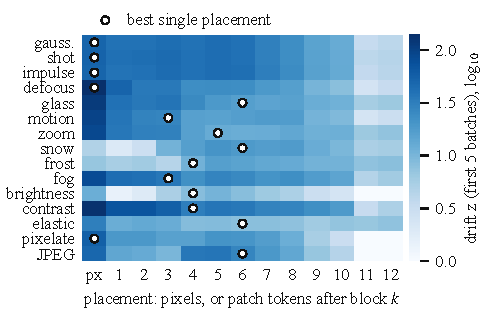
\includegraphics[width=4.5in]{../figures/drift_depth.pdf}
\caption{\textbf{Where the shift appears.} Each square gives the $z$-score of the spectral drift of the frozen tokens at one placement against the clean batches of that placement, over the first \pn{ts.dr.k} batches, averaged over severities 3 and 5 (dev cells, ViT-B/16, log scale). White dots mark the best single placement of each corruption from \cref{fig:depth}. The drift is largest at the pixels for \pn{ts.dr.pixelmax.n} of the 15 corruptions and falls with depth. The best placement does not follow it: blur and digital shifts are strongest at the pixels and best corrected at one of blocks 3 to 6, the calibration's block 6 among them.}
\label{fig:drift}
\end{figure}

\subsection{One block per shift}
\label{app:percell}
The calibration chooses one main block per shift and lets the image, not the cell, decide where to run the extra branches. A choice per cell has little room on these benchmarks: on the dev cells \tok{} plus \layer{} after the block of lowest mean entropy over the first \pn{ts.dr.k} batches of each cell gains \pn{sc.inc.choice.gain} points over the main path on ImageNet-C, against a per-cell oracle over the 13 placements of \pn{sc.inc.oracle.gain}, and the main path itself (\pn{ts.d.gain.twosite} over \neo{}) is above the oracle over all 13 single placements (\pn{ts.sel.oracleany.gain}), because the two maps correct different parts of the shift and compose. The block the calibration finds on ImageNet-C, 6, stays the most accurate block of the sweep when any one family or any one of the \pn{rb.loo.corr.n} corruptions is left out. The room left is per image, which is where the extra branches act.

\section{The Calibration}
\label{app:calib}
\subsection{What the calibration picks}
On the ImageNet-C dev predictions of ViT-B/16 the calibration picks main block \pn{rl.pick.inc.trunk} and branch blocks \pn{rl.pick.inc.lo} and \pn{rl.pick.inc.hi}, with a gain of \pn{rl.pick.inc.gain} points over the main path on the saved dev predictions (\pn{rl.sl.design.gain} when the same blocks are run on the dev cells, \cref{tab:rulesl}) against \pn{rl.pick.inc.best.gain} for the pair with the largest labelled gain on the same predictions (\pn{rl.pick.inc.best}, run held out in \cref{tab:ctl}). On ImageNet-$\overline{\text{C}}$ it picks main block \pn{rl.pick.cbar_t7.trunk} with branches after blocks \pn{rl.pick.cbar_t7.lo} and \pn{rl.pick.cbar_t7.hi}. Over all 78 sets of one or two branches (the 12 placements other than the main block as single branches, \tok{} alone among them, and their 66 pairs, while the pick itself is restricted to the 55 pairs of blocks), the entropy of the confidence-weighted average on the unsure images ranks the labelled gains with Spearman \pn{sc.inc.lf.so.rho} on ImageNet-C and \pn{sc.cb.lf.so.rho} on ImageNet-$\overline{\text{C}}$, while the disagreement with the main path does not (\pn{sc.inc.lf.so.rho.disagree} and \pn{sc.cb.lf.so.rho.disagree}).

The 0.65 quantile of the main path's entropy gives $\theta$ = \pn{rl.ss.inc.theta65}\,nat on ImageNet-C and \pn{rl.ss.cbar.theta65} on ImageNet-$\overline{\text{C}}$, and the quantile was chosen so as to reproduce the 1.5 the ViT-B/16 runs had fixed by hand. The gain is not sensitive to it: on the saved ImageNet-C dev predictions the cascade 6 / 4, 11 gains \pn{rc.theta.q04.gain} points when the branches run on \pn{rc.theta.q04.unsure}\% of the images (quantile 0.4), \pn{rc.theta.q065.gain} at \pn{rc.theta.q065.unsure}\% (0.65), \pn{rc.theta.q08.gain} at \pn{rc.theta.q08.unsure}\% (0.8) and \pn{rc.theta.q00.gain} on every image. The picks of every other pair are in \cref{tab:across} and \cref{tab:natural}. ViT-S/16, calibrated on its own images, picks \pn{rl.vs.pick.trunk} / \pn{rl.vs.pick.lo}, \pn{rl.vs.pick.hi} on ImageNet-C and gains \pn{rl.vs.both.gain} from them on its held-out set.

\subsection{Why these two blocks}
\label{app:why}
An extra branch helps only where it is right and the main path is wrong. \Cref{fig:whysites} reads this off the ImageNet-C dev predictions of ViT-B/16, where the calibration returns main block 6. On the images the main path is unsure of, the blocks next to it agree with it most (\pn{sc.inc.so.b5.agree}\% for block 5 and \pn{sc.inc.so.b7.agree}\% for block 7), so they rarely change an answer, and the shallow blocks 1 and 2 disagree most but are wrong too often (\cref{fig:whysites}a). A single branch therefore gains most from a block well away from the main block (\cref{fig:whysites}b), and two branches should also differ from each other: on the main path's errors among the unsure images, blocks 5 and 9 rescue \pn{sc.inc.so.ov.b5b9.either}\% between them and both only \pn{sc.inc.so.ov.b5b9.both}\%, while blocks 8 and 9 rescue \pn{sc.inc.so.ov.b8b9.either}\% with an overlap of \pn{sc.inc.so.ov.b8b9.both}\%. The calibration imposes none of this. It scores every pair of blocks by the entropy of the three-way average on the unsure images, and that entropy ranks the labelled gains of all 78 one- and two-branch sets with Spearman \pn{sc.inc.lf.so.rho} on ImageNet-C, so its pick, blocks 4 and 11, lies among the best pairs (\cref{fig:whysites}c), both blocks away from the main block and from each other, where the pairs are within a tenth of a point of each other. Scored with the threshold $\theta$ on the same predictions, the pick is \pn{rc.pairs.pick.rank}th of the \pn{rc.pairs.n} pairs (\pn{rc.pairs.pick.gain} points against \pn{rc.pairs.best.gain} for the best, \pn{rc.pairs.best}), above the mean pair (\pn{rc.pairs.mean}), the mean of the \pn{rc.pairs.noadj.n} pairs with no block next to the main block (\pn{rc.pairs.noadj.mean}), the two ends 1 and 12 (\pn{rc.pairs.ends112}) and the neighbours 5 and 7 (\pn{rc.pairs.adj57}). Run on the held-out set, the first pair of that ranking, \pn{rc.pairs.best}, gains \pn{rl.h.inc.b3b9.gain} points on ImageNet-C and \pn{rl.h.cbar.b3b9.gain} on ImageNet-$\overline{\text{C}}$ against \pn{rl.h.inc.b4b11.gain} and \pn{rl.h.cbar.b4b11.gain} for the pick, the two ends \pn{rl.h.inc.b1b12.gain} and \pn{rl.h.cbar.b1b12.gain} and the neighbours \pn{rl.h.inc.b5b7.gain} and \pn{rl.h.cbar.b5b7.gain} (\cref{tab:ctl}): the label-free pick matches the labelled one and both are above the pairs fixed by hand.

This is also the limit of the calibration: where it places a branch next to the main block, that block repeats the main path's answer and adds little or nothing. DeiT-B/16 picks 7 and 8 next to 6 on ImageNet-C and ImageNet-$\overline{\text{C}}$ and ViT-S/16 picks 6 and 11 around 7 on ImageNet-$\overline{\text{C}}$. Their branches add \pn{ax.deitb_inc.stack.vsbase}, \pn{ax.deitb_cbar.stack.vsbase} and \pn{ax.vits_cbar.stack.vsbase} points (\cref{tab:across}). On DeiT-B/16 and ImageNet-$\overline{\text{C}}$ block 7 alone adds \pn{ca.deitb_cbar.h.lo.gain} and block 8 alone \pn{ca.deitb_cbar.h.hi.gain}, and on ImageNet-C the pair is below block 7 alone (\pn{ca.deitb_inc.h.lo.gain}). A calibration that also asks the branches to disagree with the main path is the obvious next step and was not run.

The labelled search of \cref{app:splits} chose 5 and 9. The calibration reads no label and on held-out images is \pn{rl.h.inc.b4b11.vs59} points above those blocks on ImageNet-C and \pn{rl.h.cbar.b4b11.vs59} on ImageNet-$\overline{\text{C}}$.

\begin{figure}[!ht]
\centering
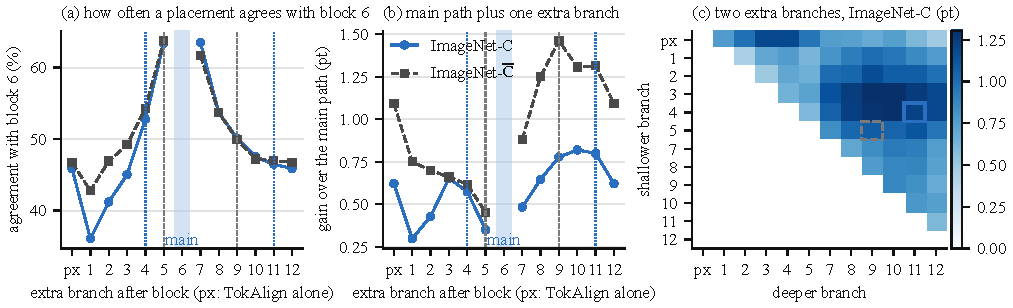
\includegraphics[width=6.75in]{../figures/why_sites.pdf}
\caption{\textbf{Why these two blocks} (dev cells, ViT-B/16, from the saved predictions, block 6 as the main block. px is \tok{} alone, a number $k$ \tok{} plus \layer{} after block $k$). (a)~The share of the main path's unsure images ($H>\theta$) on which a placement predicts the same class as the main path. (b)~The gain over the main path of the main path plus that one branch on the unsure images. (c)~The gain over the main path of the main path plus two branches on ImageNet-C, for every pair of placements (the shallower in the rows, the deeper in the columns). The calibration's pick (4, 11) is boxed solid and the pick of a labelled search (5, 9) dashed. Blocks next to the main block agree with it most and help least, and the best pairs keep their two blocks apart from the main block and from each other.}
\label{fig:whysites}
\end{figure}

\subsection{How many images the calibration needs}
\label{app:samples}
\Cref{fig:calib} repeats the calibration on the saved dev predictions with fewer images, without new runs. One calibration for a whole benchmark from the first $n$ images of every cell returns the full-sample picks from \pn{rl.ss.inc.n.same} images per cell on ImageNet-C and from \pn{rl.ss.cbar.n.same} on ImageNet-$\overline{\text{C}}$. With fewer it picks other blocks: \pn{rl.ss.inc.small.cfg} from \pn{rl.ss.inc.small.ns} images per cell on ImageNet-C (\pn{rl.ss.inc.n128.cfg} from 128), and \pn{rl.ss.cbar.n64.cfg}, \pn{rl.ss.cbar.n128.cfg}, \pn{rl.ss.cbar.n192.cfg} and \pn{rl.ss.cbar.n320.cfg} from 64, 128, 192 and 320 on ImageNet-$\overline{\text{C}}$. From 192 images per cell up, their gain on the saved predictions is within a quarter point of the full-sample picks. The picks from \pn{rl.ss.small.n} images per cell, \pn{rl.ss.inc.small.cfg} and \pn{rl.ss.cbar.small.cfg}, were run on the fourth held-out set: \pn{rl.h.inc.small.gainfull} over the full-sample main path of each benchmark on ImageNet-C and \pn{rl.h.cbar.small.gainfull} on ImageNet-$\overline{\text{C}}$, against \pn{rl.h.inc.b4b11.gainfull} and \pn{rl.h.cbar.own.gainfull} for the full-sample picks, and the pick from 192 per cell on ImageNet-$\overline{\text{C}}$ gains \pn{rl.ss.cbar.p192.held.gain} (\cref{tab:calibsize}).

One calibration per shift from the first 1, 2, 3, 5 and 10 batches of 64 images gains \pn{rl.ss.inc.k1.gain}, \pn{rl.ss.inc.k2.gain}, \pn{rl.ss.inc.k3.gain}, \pn{rl.ss.inc.k5.gain} and \pn{rl.ss.inc.k10.gain} points on ImageNet-C, so \pn{rl.ss.inc.k3.n} images of a shift are enough there. The calibration is stable in its gain, not in its exact blocks: neighbouring choices are within a quarter point of each other (\cref{fig:whysites}c). Run on fresh images, the picks of each shift's first 3 batches score \pn{rl.fs.inc.k3.stack} on ImageNet-C and \pn{rl.fs.cbar.k3.stack} on ImageNet-$\overline{\text{C}}$, \pn{rl.fs.inc.k3.vsfull} and \pn{rl.fs.cbar.k3.vsfull} from the full-sample cascade of each benchmark (\pn{rl.h.inc.b4b11} and \pn{rl.h.cbar.own}) and \pn{rl.fs.inc.k3.vsfullbase} and \pn{rl.fs.cbar.k3.vsfullbase} above the full-sample main path. The margin over the full-sample cascade comes from the main block: the per-shift main paths (\pn{rl.fs.inc.k3.base}, \pn{rl.fs.cbar.k3.base}) are above the full-sample main path by \pn{rl.fs.inc.k3.vsfullbase.base} and \pn{rl.fs.cbar.k3.vsfullbase.base}, and the branches add \pn{rl.fs.inc.k3.gain} and \pn{rl.fs.cbar.k3.gain} on top, against \pn{rl.h.inc.b4b11.gain} and \pn{rl.h.cbar.own.gainfull} for the full-sample branches. A shift-specific calibration from 192 images therefore holds on ImageNet-C and loses about half of the branch gain on ImageNet-$\overline{\text{C}}$. It runs the 13 placements once on those images, about six forward passes per image when the placements share the pass up to their block, and is paid once per shift.

\begin{figure}[!ht]
\centering
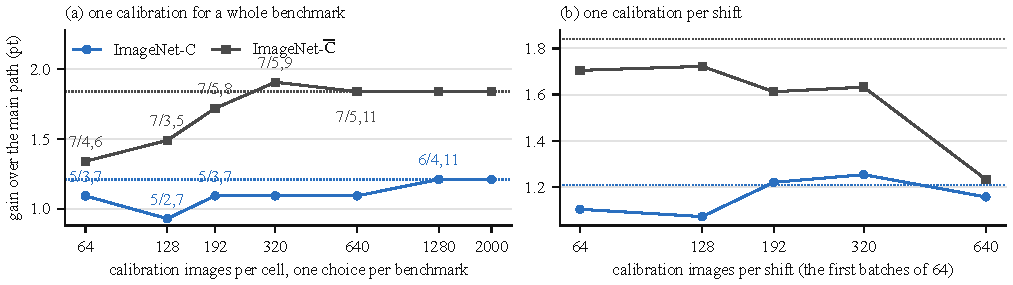
\includegraphics[width=6.75in]{../figures/calibration_size.pdf}
\caption{\textbf{How many unlabeled images the calibration needs} (the calibration repeated on the saved dev predictions, ViT-B/16, gain of the calibrated cascade over the block-6 main path on both benchmarks, in points. \Cref{tab:calibsize} moves the ImageNet-$\overline{\text{C}}$ gains to the block-7 main path). (a)~One calibration for a whole benchmark from the first $n$ images of every cell. The labels give the blocks picked (main / branches) and the dotted lines the full-sample gain. (b)~One calibration per shift from the first batches of 64 images of that shift. On ImageNet-C the gain matches the full-sample calibration from \pn{rl.ss.inc.k3.n} images per shift, on ImageNet-$\overline{\text{C}}$ it stays below it.}
\label{fig:calib}
\end{figure}

\section{The Calibrated Cascade on Held-Out Images}
\label{app:exit}
\subsection{Per corruption}
\Cref{tab:rulefam} lists the held-out cascade per ImageNet-C corruption with the share of unsure images. That share follows the main path's uncertainty: it is highest on the corruptions the main path handles worst, which is mostly where the extra branches add most (glass blur is the exception: \pn{rl.h.fam.glass_blur.routed}\% of its images run the branches for \pn{rl.h.fam.glass_blur.gain}). On ImageNet-$\overline{\text{C}}$, whose corruptions took no part in the choice, the branches add \pn{rl.h.cbar.b4b11.gain} points to the main path on the same held-out set, with gains on \pn{rl.h.cfam.wins} of the ten corruptions, the largest on plasma noise, concentric sine waves and inverse sparkles, losses on caustic refraction (\pn{rl.h.cfam.caustic_refraction.gain}) and blue noise (\pn{rl.h.cfam.blue_noise_sample.gain}), and brownish noise unchanged (\pn{rl.h.cfam.brownish_noise.gain}). One ImageNet-C corruption loses: elastic transform, \pn{rl.h.fam.elastic_transform.gain} points.

\begin{table}[!t]
\caption{\textbf{The calibrated cascade per ImageNet-C corruption} (the fourth held-out set, top-1 \% averaged over severities 3 and 5, ViT-B/16, run once). The main path is \tok{} plus \layer{} after the calibrated main block 6, the cascade adds the calibrated branches after blocks 4 and 11, gain is cascade minus main path and unsure the share of images that run the branches.}
\label{tab:rulefam}
\vskip 0.05in
\centering
\footnotesize
\begin{tabular}{l rrr r r}
\toprule
 & \multicolumn{3}{c}{top-1 \%} & & \\
\cmidrule(lr){2-4}
corruption & \neo{} & main path & cascade & gain & unsure \\
\midrule
gaussian noise & \pn{rl.h.fam.gaussian_noise.neo} & \pn{rl.h.fam.gaussian_noise.pair} & \pn{rl.h.fam.gaussian_noise.stack} & \pn{rl.h.fam.gaussian_noise.gain} & \pn{rl.h.fam.gaussian_noise.routed}\% \\
shot noise & \pn{rl.h.fam.shot_noise.neo} & \pn{rl.h.fam.shot_noise.pair} & \pn{rl.h.fam.shot_noise.stack} & \pn{rl.h.fam.shot_noise.gain} & \pn{rl.h.fam.shot_noise.routed}\% \\
impulse noise & \pn{rl.h.fam.impulse_noise.neo} & \pn{rl.h.fam.impulse_noise.pair} & \pn{rl.h.fam.impulse_noise.stack} & \pn{rl.h.fam.impulse_noise.gain} & \pn{rl.h.fam.impulse_noise.routed}\% \\
defocus blur & \pn{rl.h.fam.defocus_blur.neo} & \pn{rl.h.fam.defocus_blur.pair} & \pn{rl.h.fam.defocus_blur.stack} & \pn{rl.h.fam.defocus_blur.gain} & \pn{rl.h.fam.defocus_blur.routed}\% \\
glass blur & \pn{rl.h.fam.glass_blur.neo} & \pn{rl.h.fam.glass_blur.pair} & \pn{rl.h.fam.glass_blur.stack} & \pn{rl.h.fam.glass_blur.gain} & \pn{rl.h.fam.glass_blur.routed}\% \\
motion blur & \pn{rl.h.fam.motion_blur.neo} & \pn{rl.h.fam.motion_blur.pair} & \pn{rl.h.fam.motion_blur.stack} & \pn{rl.h.fam.motion_blur.gain} & \pn{rl.h.fam.motion_blur.routed}\% \\
zoom blur & \pn{rl.h.fam.zoom_blur.neo} & \pn{rl.h.fam.zoom_blur.pair} & \pn{rl.h.fam.zoom_blur.stack} & \pn{rl.h.fam.zoom_blur.gain} & \pn{rl.h.fam.zoom_blur.routed}\% \\
snow & \pn{rl.h.fam.snow.neo} & \pn{rl.h.fam.snow.pair} & \pn{rl.h.fam.snow.stack} & \pn{rl.h.fam.snow.gain} & \pn{rl.h.fam.snow.routed}\% \\
frost & \pn{rl.h.fam.frost.neo} & \pn{rl.h.fam.frost.pair} & \pn{rl.h.fam.frost.stack} & \pn{rl.h.fam.frost.gain} & \pn{rl.h.fam.frost.routed}\% \\
fog & \pn{rl.h.fam.fog.neo} & \pn{rl.h.fam.fog.pair} & \pn{rl.h.fam.fog.stack} & \pn{rl.h.fam.fog.gain} & \pn{rl.h.fam.fog.routed}\% \\
brightness & \pn{rl.h.fam.brightness.neo} & \pn{rl.h.fam.brightness.pair} & \pn{rl.h.fam.brightness.stack} & \pn{rl.h.fam.brightness.gain} & \pn{rl.h.fam.brightness.routed}\% \\
contrast & \pn{rl.h.fam.contrast.neo} & \pn{rl.h.fam.contrast.pair} & \pn{rl.h.fam.contrast.stack} & \pn{rl.h.fam.contrast.gain} & \pn{rl.h.fam.contrast.routed}\% \\
elastic transform & \pn{rl.h.fam.elastic_transform.neo} & \pn{rl.h.fam.elastic_transform.pair} & \pn{rl.h.fam.elastic_transform.stack} & \pn{rl.h.fam.elastic_transform.gain} & \pn{rl.h.fam.elastic_transform.routed}\% \\
pixelate & \pn{rl.h.fam.pixelate.neo} & \pn{rl.h.fam.pixelate.pair} & \pn{rl.h.fam.pixelate.stack} & \pn{rl.h.fam.pixelate.gain} & \pn{rl.h.fam.pixelate.routed}\% \\
JPEG compression & \pn{rl.h.fam.jpeg_compression.neo} & \pn{rl.h.fam.jpeg_compression.pair} & \pn{rl.h.fam.jpeg_compression.stack} & \pn{rl.h.fam.jpeg_compression.gain} & \pn{rl.h.fam.jpeg_compression.routed}\% \\
\midrule
mean & \pn{ex.h.inc.neo} & \pn{ex.h.inc.pairg} & \pn{rl.h.inc.b4b11} & \pn{rl.h.inc.b4b11.gain} & \pn{rl.h.inc.b4b11.routed}\% \\
\bottomrule
\end{tabular}
\end{table}

\subsection{Over the held-out image sets, on a stream, and in time}
\label{app:sets}
After its held-out run, the calibrated cascade was also run on three earlier ImageNet-C held-out sets and a second ImageNet-$\overline{\text{C}}$ set, each once (\cref{tab:rulesl}): over the four ImageNet-C sets it adds \pn{rl.sl.gain.lo} to \pn{rl.sl.gain.hi} points to the main path (mean \pn{rl.sl.gain.mean}).

On the continual stream of the 15 severity-5 cells of the fourth set, with exponential moving averages and no reset between cells, the cascade scores \pn{rl.st.cont.b4b11} against \pn{rl.st.cont.pairg} for the main path and \pn{rl.st.cont.neo} for \neo{}. ETA and SAR on the same stream, their weights carried across the 15 cells, score \pn{rl.st.cont.eta} and \pn{rl.st.cont.sar}, or \pn{rl.st.cont.etaneo} and \pn{rl.st.cont.sarneo} with \neo{}, so over the long stream the cascade stays \pn{rl.st.cont.cascade.vs.etaneo} points above ETA with \neo{} without a gradient. The main path inside ETA scores \pn{rl.st.cont.etamain} (\pn{rl.st.cont.etamainneo} with \neo{}), \pn{rl.st.cont.etamain.vscascade} above the cascade. On the clean-return stream, which alternates clean and corrupted segments, the cascade's clean segments score \pn{rl.st.cr.b4b11} against \pn{rl.st.cr.neo} for \neo{}, \pn{rl.st.cr.eta} for ETA and \pn{rl.st.cr.sar} for SAR, so the gate keeps the cascade inert on clean images.

Timed on six dev cells with CUDA synchronization, a batch of 64 takes \pn{rl.cost.neo.ms}\,ms with \neo{}, \pn{rl.cost.pair.ms} with the main path (\pn{rl.cost.pair.x} times) and \pn{rl.cost.b4b11.ms} with the calibrated cascade (\pn{rl.cost.b4b11.x} times). ETA takes \pn{rl.cost.eta.x} times \neo{}'s time on the same cells, SAR \pn{rl.cost.sar.x}, PEA \pn{rl.cost.pea.x} (\pn{rl.cost.peaviews.x} with its views) and FOA \pn{rl.cost.foa.x} (\cref{tab:others}).

\begin{table}[!ht]
\caption{\textbf{The calibrated cascade over image sets} (top-1 \%, ViT-B/16, blocks 6 / 4, 11 calibrated on the ImageNet-C dev images, each held-out set run once, gains against the main path and \neo{} of the same set). The four ImageNet-C held-out sets are disjoint 2{,}000-image sets per cell. The fourth is the set of \cref{tab:exit}.}
\label{tab:rulesl}
\vskip 0.05in
\centering
\footnotesize
\begin{tabular}{l rr r r r}
\toprule
 & \multicolumn{3}{c}{top-1 \%} & \multicolumn{2}{c}{gain of the cascade} \\
\cmidrule(lr){2-4}\cmidrule(lr){5-6}
image set & \neo{} & main path & cascade & over main path & over \neo{} \\
\midrule
ImageNet-C, dev & \pn{rl.sl.design.neo} & \pn{rl.sl.design.pair} & \pn{rl.sl.design.b4b11} & \pn{rl.sl.design.gain} & \pn{rl.sl.design.gainneo} \\
ImageNet-C, first held-out set & \pn{rl.sl.heldout.neo} & \pn{rl.sl.heldout.pair} & \pn{rl.sl.heldout.b4b11} & \pn{rl.sl.heldout.gain} & \pn{rl.sl.heldout.gainneo} \\
ImageNet-C, second & \pn{rl.sl.heldout2.neo} & \pn{rl.sl.heldout2.pair} & \pn{rl.sl.heldout2.b4b11} & \pn{rl.sl.heldout2.gain} & \pn{rl.sl.heldout2.gainneo} \\
ImageNet-C, third & \pn{rl.sl.heldout3.neo} & \pn{rl.sl.heldout3.pair} & \pn{rl.sl.heldout3.b4b11} & \pn{rl.sl.heldout3.gain} & \pn{rl.sl.heldout3.gainneo} \\
ImageNet-C, fourth (\cref{tab:exit}) & \pn{ex.h.inc.neo} & \pn{ex.h.inc.pairg} & \pn{rl.h.inc.b4b11} & \pn{rl.h.inc.b4b11.gain} & \pn{rl.h.inc.b4b11.gainneo} \\
\midrule
ImageNet-$\overline{\text{C}}$, dev & \pn{rl.sl.cbar_design.neo} & \pn{rl.sl.cbar_design.pair} & \pn{rl.sl.cbar_design.b4b11} & \pn{rl.sl.cbar_design.gain} & \pn{rl.sl.cbar_design.gainneo} \\
ImageNet-$\overline{\text{C}}$, third held-out set & \pn{rl.sl.cbar_heldout3.neo} & \pn{rl.sl.cbar_heldout3.pair} & \pn{rl.sl.cbar_heldout3.b4b11} & \pn{rl.sl.cbar_heldout3.gain} & \pn{rl.sl.cbar_heldout3.gainneo} \\
ImageNet-$\overline{\text{C}}$, fourth (\cref{tab:exit}) & \pn{ex.h.cb.neo} & \pn{ex.h.cb.pairg} & \pn{rl.h.cbar.b4b11} & \pn{rl.h.cbar.b4b11.gain} & \pn{rl.h.cbar.b4b11.gainneo} \\
\bottomrule
\end{tabular}
\end{table}

\subsection{Ablations and controls}
\label{app:controls}
\Cref{tab:ctl} collects the ablations and controls, each run once on the fourth held-out set. The branch after block 4 alone adds \pn{rl.h.inc.b4.gain} and \pn{rl.h.cbar.b4.gain} points to the main path, the branch after block 11 alone \pn{rl.h.inc.b11.gain} and \pn{rl.h.cbar.b11.gain}, both together \pn{rl.h.inc.b4b11.gain} and \pn{rl.h.cbar.b4b11.gain}, so the two add. Running the branches on the same share of images chosen at random, instead of the images the main path is unsure of, keeps \pn{rl.ctl.inc.random.gain} of the \pn{rl.h.inc.b4b11.gain} points on ImageNet-C and \pn{rl.ctl.cbar.random.gain} of \pn{rl.h.cbar.b4b11.gain} on ImageNet-$\overline{\text{C}}$: the confidence picks the images that benefit. Averaging the main path over three views of the same unsure images (the image, its horizontal flip and the central 192 pixels resized to 224, with the maps of the batch frozen and one \neo{} mean per view), an ensemble over views instead of over placements, gains \pn{rl.ctl.inc.views.gain} and \pn{rl.ctl.cbar.views.gain} at two more full passes on those images, against the 14 of 12 blocks the two branches re-run (\cref{alg:stack}), so \pn{rl.ctl.inc.views.share}\% and \pn{rl.ctl.cbar.views.share}\% of the branches' gain is averaging and the rest comes from where the map acts.

With blocks 5 and 9, which were run with more controls, equal weights instead of confidence weights change the result by \pn{ex.ctl.inc.equal.vsmethod} and \pn{ex.ctl.cb.equal.vsmethod} points, so the weighting matters little, and running the branches on every image adds \pn{ex.ctl.inc.full.vsmethod} and \pn{ex.ctl.cb.full.vsmethod} points more at about three times the extra cost. On the saved dev predictions, running the branches on the most confident images instead gives \pn{sc.inc.ctl.most_confident_routed_same_fraction} points, and an oracle that runs them exactly on the main path's errors would give \pn{sc.inc.ctl.oracle_routing_trunk_errors}, the ceiling of this design.

\begin{table}[!ht]
\caption{\textbf{Ablations and controls} (top-1 points over the main path, the fourth held-out set, ViT-B/16, each variant run once. Unsure is the share of images that run the extra branches and clean the clean cell against \neo{}. Bold: the best in the column). Upper block: the calibrated cascade, its branches alone, the random control, the main path averaged over three views (the image, its flip, a center crop) of the same unsure images, the pair the labelled dev search ranks first and two pairs fixed by hand. Lower block: the cascade with blocks 5 and 9, run with more controls.}
\label{tab:ctl}
\vskip 0.05in
\centering
\footnotesize
\begin{tabular}{l rr rr r}
\toprule
 & \multicolumn{2}{c}{ImageNet-C} & \multicolumn{2}{c}{ImageNet-$\overline{\text{C}}$} & \\
\cmidrule(lr){2-3}\cmidrule(lr){4-5}
variant & gain & unsure & gain & unsure & clean \\
\midrule
\textbf{calibrated cascade, blocks 6 / 4, 11} & \textbf{\pn{rl.h.inc.b4b11.gain}} & \pn{rl.h.inc.b4b11.routed}\% & \pn{rl.h.cbar.b4b11.gain} & \pn{rl.h.cbar.b4b11.routed}\% & \pn{rl.h.inc.b4b11.cleand} \\
\quad branch 4 only & \pn{rl.h.inc.b4.gain} & \pn{rl.h.inc.b4.routed}\% & \pn{rl.h.cbar.b4.gain} & \pn{rl.h.cbar.b4.routed}\% & \pn{rl.h.inc.b4.cleand} \\
\quad branch 11 only & \pn{rl.h.inc.b11.gain} & \pn{rl.h.inc.b11.routed}\% & \pn{rl.h.cbar.b11.gain} & \pn{rl.h.cbar.b11.routed}\% & \pn{rl.h.inc.b11.cleand} \\
\quad random images, same share & \pn{rl.ctl.inc.random.gain} & \pn{rl.ctl.inc.random.routed}\% & \pn{rl.ctl.cbar.random.gain} & \pn{rl.ctl.cbar.random.routed}\% & \pn{ex.ctl.inc.random.clean} \\
\quad three views of the main path, same images & \pn{rl.ctl.inc.views.gain} & \pn{rl.ctl.inc.views.routed}\% & \pn{rl.ctl.cbar.views.gain} & \pn{rl.ctl.cbar.views.routed}\% & \pn{rl.ctl.inc.views.cleand} \\
\quad blocks 6 / 3, 9 (best pair on the dev labels) & \textbf{\pn{rl.h.inc.b3b9.gain}} & \pn{rl.h.inc.b3b9.routed}\% & \pn{rl.h.cbar.b3b9.gain} & \pn{rl.h.cbar.b3b9.routed}\% & \pn{rl.h.inc.b3b9.cleand} \\
\quad blocks 6 / 1, 12 (the two ends) & \pn{rl.h.inc.b1b12.gain} & \pn{rl.h.inc.b1b12.routed}\% & \pn{rl.h.cbar.b1b12.gain} & \pn{rl.h.cbar.b1b12.routed}\% & \pn{rl.h.inc.b1b12.cleand} \\
\quad blocks 6 / 5, 7 (the neighbours) & \pn{rl.h.inc.b5b7.gain} & \pn{rl.h.inc.b5b7.routed}\% & \pn{rl.h.cbar.b5b7.gain} & \pn{rl.h.cbar.b5b7.routed}\% & \pn{rl.h.inc.b5b7.cleand} \\
\midrule
cascade with blocks 6 / 5, 9 & \pn{ex.h.inc.gaing.b5b9g} & \pn{ex.h.inc.routed.b5b9g}\% & \pn{ex.h.cb.gaing.b5b9g} & \pn{ex.h.cb.routed.b5b9g}\% & \pn{ex.h.clean.vsneo.b5b9g} \\
\quad random images, same share & \pn{ex.ctl.inc.random.gaing} & \pn{ex.ctl.inc.random.routed}\% & \pn{ex.ctl.cb.random.gaing} & \pn{ex.ctl.cb.random.routed}\% & \pn{ex.ctl.inc.random.clean} \\
\quad equal weights & \pn{ex.ctl.inc.equal.gaing} & \pn{ex.ctl.inc.equal.routed}\% & \pn{ex.ctl.cb.equal.gaing} & \pn{ex.ctl.cb.equal.routed}\% & \pn{ex.ctl.inc.equal.clean} \\
\quad every image & \textbf{\pn{ex.ctl.inc.full.gaing}} & \pn{ex.ctl.inc.full.routed}\% & \textbf{\pn{ex.ctl.cb.full.gaing}} & \pn{ex.ctl.cb.full.routed}\% & \pn{ex.ctl.inc.full.clean} \\
\bottomrule
\end{tabular}
\end{table}

\subsection{The main path inside ETA and SAR}
\label{app:base}
The main path is the cascade without its extra branches. Inside ETA it adds \pn{ts.hb.gain.etatwosite.over.etaneo} points to ETA with \neo{} on ViT-B/16 and \pn{ts.hs.gain.etatwosite.over.etaneo} on ViT-S/16 on the third held-out set, and \pn{ts.sl.gain.etatwosite.over.etaneo.lo} to \pn{ts.sl.gain.etatwosite.over.etaneo.hi} over three disjoint held-out sets of ViT-B/16. With the frozen network it gains \pn{ts.sl.gain.twosite.lo} to \pn{ts.sl.gain.twosite.hi} over \neo{} on the same sets, with the clean cell within \pn{ts.sl.clean.twosite.hi} points. Inside SAR \citep{sar2023}, with the two maps in front of it exactly as in front of ETA (official code, batch 64, fresh weights per cell), the main path adds \pn{sar.ts.h.neo.gain.px} points on top of \tok{} with \neo{} on the held-out cells.

With the whole cascade inside ETA (the last column of \cref{tab:across}), ETA adapts on the main path's logits and the unsure images also run the two branches with the same current weights: it is above ETA with the main path inside on all fourteen pairs of \cref{tab:across} and \cref{tab:natural}, by \pn{ax.vitb_inc.etastack.vsetaours}, \pn{ax.vits_inc.etastack.vsetaours}, \pn{ax.vitb_cbar.etastack.vsetaours} and \pn{ax.vits_cbar.etastack.vsetaours} points on the AugReg ViTs and the corruptions and \pn{ax.deitb_inc.etastack.vsetaours}, \pn{ax.deitb_cbar.etastack.vsetaours}, \pn{ax.deitb_r.etastack.vsetaours} and \pn{ax.deitb_sketch.etastack.vsetaours} on DeiT-B/16. The margin is smallest on ViT-B/16 $\times$ Sketch (\pn{ax.vitb_sketch.etastack.vsetaours}, a tie), where \layer{} adds little, and on DeiT-B/16 $\times$ ImageNet-C, where the branches sit next to the main block. Its clean cell is within \pn{ax.vits_inc.etastack.cleand} of ETA with \neo{} on the four corruption pairs of the AugReg ViTs, and between \pn{ax.vitb_sketch.etastack.cleand} (ViT-B/16 $\times$ Sketch and DeiT-B/16 $\times$ ImageNet-C) and \pn{ax.deitb_sketch.etastack.cleand} (DeiT-B/16 $\times$ Sketch) on the other ten pairs.

\subsection{Uncertainty of the held-out gains}
\label{app:ci}
Every number of this report is one run, so \cref{tab:ci} gives, for every row of \cref{tab:across} and \cref{tab:natural}, the gain of the calibrated cascade over the main path with a 95\% interval from a paired bootstrap over the held-out images (\pn{rc.bootstrap} draws, the same images for both arms) and over the cells. The branch gains are above zero on \pn{rc.corr.n} of the \pn{rc.corr.n} corruption pairs over images, over cells the interval includes zero on \pn{rc.corr.cic.zero.n} of them (\pn{rc.corr.cic.zero.names}, where a branch sits next to the main block), and on the three-cell natural pairs the interval is up to $\pm$\pn{rc.nat.half.max} points wide. For \cref{tab:exit} the cascade 6 / 4, 11 gains \pn{rc.t1.inc.gain} [\pn{rc.t1.inc.ci.lo}, \pn{rc.t1.inc.ci.hi}] over the main path on ImageNet-C and \pn{rc.t1.cbar.gain} [\pn{rc.t1.cbar.ci.lo}, \pn{rc.t1.cbar.ci.hi}] on ImageNet-$\overline{\text{C}}$, changing the answer on \pn{rc.t1.inc.changed}\% and \pn{rc.t1.cbar.changed}\% of the images (\pn{rc.t1.inc.fixed}\% fixed and \pn{rc.t1.inc.broken}\% broken on ImageNet-C). The table also gives the Spearman correlation of \cref{fig:signalgrid} without blocks 1 to 3, and the entropy the picked placement saves against \tok{} alone on the dev images.

\begin{table}[!t]
\caption{\textbf{Intervals of the held-out gains} (the calibrated cascade minus the main path in top-1 points, the held-out set of each row of \cref{tab:across} and \cref{tab:natural}, with 95\% intervals from a paired bootstrap over images and over cells). $\rho$: the Spearman correlation of mean entropy and accuracy over the 13 placements on dev images, and over \tok{} alone and blocks 4 to 12. Saved: the mean entropy of \tok{} alone minus that of the picked placement on the dev images, in nat. Gap: the accuracy of the picked placement minus that of the most accurate one on the dev images.}
\label{tab:ci}
\vskip 0.05in
\centering
\footnotesize
\setlength{\tabcolsep}{4pt}
\begin{tabular}{ll r r c c rr r r}
\toprule
model & shift & cells & gain & 95\% over images & 95\% over cells & $\rho$ & $\rho$ (4--12) & saved & gap \\
\midrule
ViT-B/16 & ImageNet-C & \pn{rc.vitb_inc.n} & \pn{rc.vitb_inc.gain} & [\pn{rc.vitb_inc.ci.lo}, \pn{rc.vitb_inc.ci.hi}] & [\pn{rc.vitb_inc.cic.lo}, \pn{rc.vitb_inc.cic.hi}] & \pn{rc.vitb_inc.rho} & \pn{rc.vitb_inc.rho4} & \pn{rc.vitb_inc.saved} & \pn{rc.vitb_inc.gap} \\
ViT-B/16 & ImageNet-$\overline{\text{C}}$ & \pn{rc.vitb_cbar.n} & \pn{rc.vitb_cbar.gain} & [\pn{rc.vitb_cbar.ci.lo}, \pn{rc.vitb_cbar.ci.hi}] & [\pn{rc.vitb_cbar.cic.lo}, \pn{rc.vitb_cbar.cic.hi}] & \pn{rc.vitb_cbar.rho} & \pn{rc.vitb_cbar.rho4} & \pn{rc.vitb_cbar.saved} & \pn{rc.vitb_cbar.gap} \\
ViT-B/16 & ImageNet-R & \pn{rc.vitb_r.n} & \pn{rc.vitb_r.gain} & [\pn{rc.vitb_r.ci.lo}, \pn{rc.vitb_r.ci.hi}] & [\pn{rc.vitb_r.cic.lo}, \pn{rc.vitb_r.cic.hi}] & \pn{rc.vitb_r.rho} & \pn{rc.vitb_r.rho4} & \pn{rc.vitb_r.saved} & \pn{rc.vitb_r.gap} \\
ViT-B/16 & Sketch & \pn{rc.vitb_sketch.n} & \pn{rc.vitb_sketch.gain} & [\pn{rc.vitb_sketch.ci.lo}, \pn{rc.vitb_sketch.ci.hi}] & [\pn{rc.vitb_sketch.cic.lo}, \pn{rc.vitb_sketch.cic.hi}] & \pn{rc.vitb_sketch.rho} & \pn{rc.vitb_sketch.rho4} & \pn{rc.vitb_sketch.saved} & \pn{rc.vitb_sketch.gap} \\
\midrule
ViT-S/16 & ImageNet-C & \pn{rc.vits_inc.n} & \pn{rc.vits_inc.gain} & [\pn{rc.vits_inc.ci.lo}, \pn{rc.vits_inc.ci.hi}] & [\pn{rc.vits_inc.cic.lo}, \pn{rc.vits_inc.cic.hi}] & \pn{rc.vits_inc.rho} & \pn{rc.vits_inc.rho4} & \pn{rc.vits_inc.saved} & \pn{rc.vits_inc.gap} \\
ViT-S/16 & ImageNet-$\overline{\text{C}}$ & \pn{rc.vits_cbar.n} & \pn{rc.vits_cbar.gain} & [\pn{rc.vits_cbar.ci.lo}, \pn{rc.vits_cbar.ci.hi}] & [\pn{rc.vits_cbar.cic.lo}, \pn{rc.vits_cbar.cic.hi}] & \pn{rc.vits_cbar.rho} & \pn{rc.vits_cbar.rho4} & \pn{rc.vits_cbar.saved} & \pn{rc.vits_cbar.gap} \\
ViT-S/16 & ImageNet-R & \pn{rc.vits_r.n} & \pn{rc.vits_r.gain} & [\pn{rc.vits_r.ci.lo}, \pn{rc.vits_r.ci.hi}] & [\pn{rc.vits_r.cic.lo}, \pn{rc.vits_r.cic.hi}] & \pn{rc.vits_r.rho} & \pn{rc.vits_r.rho4} & \pn{rc.vits_r.saved} & \pn{rc.vits_r.gap} \\
ViT-S/16 & Sketch & \pn{rc.vits_sketch.n} & \pn{rc.vits_sketch.gain} & [\pn{rc.vits_sketch.ci.lo}, \pn{rc.vits_sketch.ci.hi}] & [\pn{rc.vits_sketch.cic.lo}, \pn{rc.vits_sketch.cic.hi}] & \pn{rc.vits_sketch.rho} & \pn{rc.vits_sketch.rho4} & \pn{rc.vits_sketch.saved} & \pn{rc.vits_sketch.gap} \\
\midrule
DeiT-B/16 & ImageNet-C & \pn{rc.deitb_inc.n} & \pn{rc.deitb_inc.gain} & [\pn{rc.deitb_inc.ci.lo}, \pn{rc.deitb_inc.ci.hi}] & [\pn{rc.deitb_inc.cic.lo}, \pn{rc.deitb_inc.cic.hi}] & \pn{rc.deitb_inc.rho} & \pn{rc.deitb_inc.rho4} & \pn{rc.deitb_inc.saved} & \pn{rc.deitb_inc.gap} \\
DeiT-B/16 & ImageNet-$\overline{\text{C}}$ & \pn{rc.deitb_cbar.n} & \pn{rc.deitb_cbar.gain} & [\pn{rc.deitb_cbar.ci.lo}, \pn{rc.deitb_cbar.ci.hi}] & [\pn{rc.deitb_cbar.cic.lo}, \pn{rc.deitb_cbar.cic.hi}] & \pn{rc.deitb_cbar.rho} & \pn{rc.deitb_cbar.rho4} & \pn{rc.deitb_cbar.saved} & \pn{rc.deitb_cbar.gap} \\
DeiT-B/16 & ImageNet-R & \pn{rc.deitb_r.n} & \pn{rc.deitb_r.gain} & [\pn{rc.deitb_r.ci.lo}, \pn{rc.deitb_r.ci.hi}] & [\pn{rc.deitb_r.cic.lo}, \pn{rc.deitb_r.cic.hi}] & \pn{rc.deitb_r.rho} & \pn{rc.deitb_r.rho4} & \pn{rc.deitb_r.saved} & \pn{rc.deitb_r.gap} \\
DeiT-B/16 & Sketch & \pn{rc.deitb_sketch.n} & \pn{rc.deitb_sketch.gain} & [\pn{rc.deitb_sketch.ci.lo}, \pn{rc.deitb_sketch.ci.hi}] & [\pn{rc.deitb_sketch.cic.lo}, \pn{rc.deitb_sketch.cic.hi}] & \pn{rc.deitb_sketch.rho} & \pn{rc.deitb_sketch.rho4} & \pn{rc.deitb_sketch.saved} & \pn{rc.deitb_sketch.gap} \\
\midrule
DeiT-S/16 & ImageNet-C & \pn{rc.deits_inc.n} & \pn{rc.deits_inc.gain} & [\pn{rc.deits_inc.ci.lo}, \pn{rc.deits_inc.ci.hi}] & [\pn{rc.deits_inc.cic.lo}, \pn{rc.deits_inc.cic.hi}] & \pn{rc.deits_inc.rho} & \pn{rc.deits_inc.rho4} & \pn{rc.deits_inc.saved} & \pn{rc.deits_inc.gap} \\
DeiT-S/16 & ImageNet-$\overline{\text{C}}$ & \pn{rc.deits_cbar.n} & \pn{rc.deits_cbar.gain} & [\pn{rc.deits_cbar.ci.lo}, \pn{rc.deits_cbar.ci.hi}] & [\pn{rc.deits_cbar.cic.lo}, \pn{rc.deits_cbar.cic.hi}] & \pn{rc.deits_cbar.rho} & \pn{rc.deits_cbar.rho4} & \pn{rc.deits_cbar.saved} & \pn{rc.deits_cbar.gap} \\
DeiT-S/16 & ImageNet-R & \pn{rc.deits_r.n} & \pn{rc.deits_r.gain} & [\pn{rc.deits_r.ci.lo}, \pn{rc.deits_r.ci.hi}] & [\pn{rc.deits_r.cic.lo}, \pn{rc.deits_r.cic.hi}] & \pn{rc.deits_r.rho} & \pn{rc.deits_r.rho4} & \pn{rc.deits_r.saved} & \pn{rc.deits_r.gap} \\
DeiT-S/16 & Sketch & \pn{rc.deits_sketch.n} & \pn{rc.deits_sketch.gain} & [\pn{rc.deits_sketch.ci.lo}, \pn{rc.deits_sketch.ci.hi}] & [\pn{rc.deits_sketch.cic.lo}, \pn{rc.deits_sketch.cic.hi}] & \pn{rc.deits_sketch.rho} & \pn{rc.deits_sketch.rho4} & \pn{rc.deits_sketch.saved} & \pn{rc.deits_sketch.gap} \\
\bottomrule
\end{tabular}
\end{table}

\subsection{Against other test-time adaptation methods}
\label{app:others}
\Cref{tab:others} places the main path and the calibrated cascade next to the gradient-free \neo{}, PEA and FOA and the gradient-based ETA and SAR on the 30 ImageNet-C dev cells (FOA on 15 severity-5 cells with 6k-image streams), each with the official code (settings in \cref{app:settings}), alone and with \tok{} in front. \tok{} adds \pn{u.range.lo} to \pn{u.range.hi} points to every method (\pn{u.peaviews.gain} to PEA with its views) and keeps the clean cell within \pn{u.cleanmax} points. The calibrated cascade, with no gradient, is above ETA with \neo{} and SAR with \neo{} at \pn{rl.cost.b4b11.x} times \neo{}'s time against ETA's \pn{rl.cost.eta.x}. \Cref{fig:frontier} draws accuracy against GMACs per image and against time per batch on the six timing cells for every method of \cref{tab:others}: the main path costs about as much as \neo{}, the cascade adds the branches on a third of the images, and every gradient-based or search-based method is both costlier and less accurate.

\begin{table}[!ht]
\caption{\textbf{Against other TTA methods} (top-1 \%, ViT-B/16, the 30 ImageNet-C dev cells, official code, one run). Gradient-free methods run forward passes only. The gradient-based ones backpropagate entropy. ``$+$ \tok{}'' puts \tok{} in front of the method. Compute: GMACs per image, where one forward pass of ViT-B/16 is 17.56 GMACs, counting one $d{\times}d$ multiply per token for each map, the branches on the unsure share of the images, a backward pass as two forward passes (ETA one of each, SAR two of each), PEA's two passes with a map after every block (times three views) and FOA's 28 forward passes per batch (27 prompts plus the model). Time: per batch relative to \neo{} on six dev cells, our methods, ETA and SAR in one run and PEA and FOA in a second run with its own \neo{} reference. The main path and the cascade contain \tok{} (--). Bold: the best in the column. FOA runs on 15 severity-5 cells with 6k-image streams, not on the same images (\cref{app:settings}). PEA uses 20k source images, without or with three augmented views of each test image.}
\label{tab:others}
\vskip 0.05in
\centering
\footnotesize
\setlength{\tabcolsep}{4pt}
\begin{tabular}{l r r r r}
\toprule
 & \multicolumn{2}{c}{top-1 \%} & & \\
\cmidrule(lr){2-3}
method & alone & $+$ \tok{} & compute & time \\
\midrule
\multicolumn{5}{l}{\textit{gradient-free}} \\
\neo{} \citep{neo2026} & \pn{u.neo.alone} & \pn{u.neo.tok} & \pn{rl.macs.neo} & \pn{rl.cost.neo.x} \\
PEA \citep{pea2026} & \pn{u.pea.alone} & \pn{u.pea.tok} & \pn{rl.macs.pea} & \pn{rl.cost.pea.x} \\
PEA with views & \pn{u.peaviews.alone} & \pn{u.peaviews.tok} & \pn{rl.macs.peaviews} & \pn{rl.cost.peaviews.x} \\
FOA \citep{foa2024} & \pn{u.foa.alone} & \pn{u.foa.tok} & \pn{rl.macs.foa} & \pn{rl.cost.foa.x} \\
the main path (ours) & \pn{ts.d.twosite} & -- & \pn{rl.macs.pair} & \pn{rl.cost.pair.x} \\
\textbf{the calibrated cascade (ours)} & \textbf{\pn{rl.sl.design.b4b11}} & -- & \pn{rl.macs.b4b11} & \pn{rl.cost.b4b11.x} \\
\midrule
\multicolumn{5}{l}{\textit{gradient-based}} \\
ETA with \neo{} \citep{eata2022} & \pn{u.eta.alone} & \textbf{\pn{u.eta.tok}} & \pn{rl.macs.eta} & \pn{rl.cost.eta.x} \\
SAR with \neo{} \citep{sar2023} & \pn{u.sar.alone} & \pn{u.sar.tok} & \pn{rl.macs.sar} & \pn{rl.cost.sar.x} \\
\bottomrule
\end{tabular}
\end{table}

\begin{figure}[!ht]
\centering
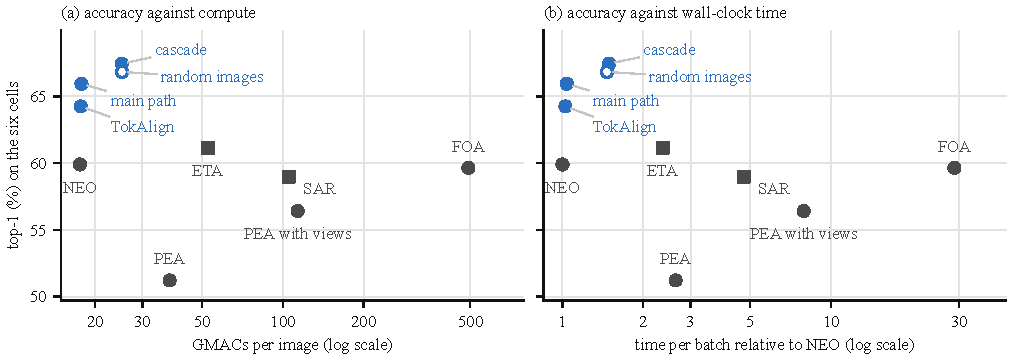
\includegraphics[width=6.75in]{../figures/frontier.pdf}
\caption{\textbf{Accuracy against compute and against time} (ViT-B/16, the six ImageNet-C dev cells of the timing run, batch 64, log scales). (a)~GMACs per image, counted as in \cref{tab:others}. (b)~Time per batch relative to \neo{}, one timed run per method. Blue: ours, \tok{}, the main path and the cascade, which run forward passes only. Hollow: random images, the control that runs the branches on the same share of images chosen at random. Grey circles: \neo{}, PEA and FOA, gradient-free with the official code. Grey squares: the gradient-based ETA and SAR.}
\label{fig:frontier}
\end{figure}

\section{Limitations}
\label{app:limits}
\subsection{The calibration assumes the shifts it reads are the shifts it will see}
The three blocks and $\theta$ are chosen from unlabeled images of the target distribution and then fixed, so the method assumes that the test images come from the same shifts as the calibration images. The report measures how far this can be relaxed. Blocks calibrated on ImageNet-C transfer to ImageNet-$\overline{\text{C}}$, which took no part in the calibration, with \pn{rl.h.cbar.b4b11} top-1 against \pn{rl.h.cbar.own} for blocks calibrated on ImageNet-$\overline{\text{C}}$ itself (\cref{app:samples}). Natural shifts need their own calibration, and on the AugReg ViTs no calibration helps on renditions and little on sketches (\cref{tab:across} and \cref{tab:natural}).

On the continual stream of \cref{app:sets} the fixed blocks hold because every corruption of the stream was in the calibration pool. A stream that moves to a shift outside that pool keeps the blocks it has: the calibration has no step that notices the change, and re-calibrating costs the 13 placements on a few hundred images of the new shift (\cref{app:samples}). An online calibration is future work.

\subsection{Scope}
\label{app:scope}
Every result is on ViT-family backbones of 12 blocks at 224 pixels, on batches of 64, with source statistics from 3{,}000 clean images. The cascade costs \pn{rl.cost.b4b11.x} times the time of \neo{}, the branches running on about a third of the images, the map needs a covariance per placement (\cref{app:settings}), and the calibration runs the 13 placements once on a few hundred images per shift (\cref{app:samples}). ETA and SAR start from fresh weights on every 2{,}000-image cell, 31 batches, a protocol that favours methods which converge in a few batches, as the closed-form maps do. Under it ETA with \neo{} ends below \neo{} on DeiT-B/16 $\times$ ImageNet-$\overline{\text{C}}$ (\pn{ax.deitb_cbar.eta} in \cref{tab:across}). On the continual stream of \cref{app:sets}, where their weights carry across 15 cells, the cascade stays \pn{rl.st.cont.cascade.vs.etaneo} and \pn{rl.st.cont.cascade.vs.sarneo} points above ETA and SAR with \neo{}.

\section{What Did Not Work}
\label{app:negatives}
\paragraph{Choosing the block from the drift.} The two drift rules of \cref{app:drift} fall \pn{ts.sel.drift2.gain} and \pn{ts.sel.driftany.gain} points over \neo{} against \pn{ts.d.gain.twosite} for the main path, because the drift is largest at the pixels for almost every corruption (\cref{fig:drift}).

\paragraph{One choice per cell.} Choosing the block per cell by the entropy of its first batches gains \pn{sc.inc.choice.gain} points over the main path on ImageNet-C, against a per-cell oracle of \pn{sc.inc.oracle.gain}: the cells agree on the block (\cref{app:percell}). The per-image extra branches gain more (\pn{rl.h.inc.b4b11.gain}).

\paragraph{Other maps.} Re-centering every block's token mean toward the source lowers top-1 from \pn{blk.neo}\% with \neo{} to \pn{blk.all}\% on the dev cells, so the map must stay away from the early blocks, which the entropy does on its own. A two-level map that whitens the between-image and the within-image part of a placement's covariance separately is within \pn{hi.d.hierb6.vs.b6} points of the pooled map of \cref{eq:map} after the calibrated main block and was not kept.

\paragraph{Natural shifts on the AugReg ViTs.} For ViT-B/16 and ViT-S/16 \layer{} helps at no block on ImageNet-R, and on ImageNet-Sketch only a late block helps (block 11: \pn{ax.vitb_sketch.base} over \neo{} for ViT-B/16, which the entropy finds, and \pn{ca.vits_sketch.best.gainneo} for ViT-S/16, which picks block 6 instead), so the entropy picks a more confident, less accurate block in three of four pairs. The DeiT models gain on renditions, and DeiT-B/16 also on sketches, where DeiT-S/16 misses a block worth under a point (\cref{tab:natural}). A criterion that can also choose ``no \layer{}'' is the open question this leaves.

\section{Settings and Licenses}
\label{app:settings}
\paragraph{The map.} $\lambda{=}0.1$ and a prior of four images' worth of vectors at every placement. The statistics are kept in float32 and the eigendecomposition refreshed every 16 batches on streams. The running means use an exponential moving average on streams (0.2 at the pixels, 0.5 for \neo{}) and plain averages within a cell. The number of clean source images is the one strong sensitivity: with 50 images \tok{} collapses to \pn{abl.src50}\% and with 300 it stays at \pn{abl.src300}\%, below \neo{}, so 3{,}000 are used throughout. Each map costs one $d{\times}d$ multiply per token, about 1.5\% of a ViT-B/16 forward pass of \pn{cost.gmacs} GMACs for the main path. The gate thresholds 0.4 (DCT power) and 0.3 (mean) were set on clean dev batches.

\paragraph{ETA and SAR.} ETA is EATA without its Fisher term, run with the official code, learning rate 0.001 at batch 64 and fresh weights per cell, so 31 gradient steps per cell (\cref{app:scope}). Its entropy margin is scaled to the number of classes on ImageNet-R. With the cascade inside it, ETA's forward pass is the main path, so it adapts on the main path's logits exactly as with the main path alone. The unsure images also run the two branches with the same current weights, without gradients. SAR ran with its official code at batch 64 and fresh weights per cell. On the streams of \cref{app:sets} both keep their weights across the cells, and their rows with \neo{} apply \neo{} to the recorded input of the head.

\paragraph{FOA.} FOA ran with its official code and configuration: 3 prompt tokens, a CMA-ES population of 27 plus 1, $\lambda{=}0.4$ and activation shifting. Its source statistics came from our 3{,}000 clean source images, and it was reset per cell. It scores \pn{foa.2k}\% on 2{,}000-image cells (15 severity-5 cells, where \neo{} scores \pn{foa.2k.neo}\%) and \pn{foa.6k}\% on 6{,}000-image cells. Its paper reports 66.3\% on 50{,}000-image domains, which give the evolutionary search 25 times more batches to converge.

\paragraph{PEA.} PEA ran with its official code: grouped CORAL after every block, EMA 0.02, drift and entropy resets, and optional views. Its source statistics came from 3{,}000 and from 20{,}000 unlabeled clean validation images. It scores \pn{pea.3k}\% and \pn{pea.20k}\% without views and \pn{pea.3k.views}\% and \pn{pea.20k.views}\% with three views, against \pn{pea.source}\% for the unadapted model. Four differences from its paper could not be removed: the augreg instead of augreg2 weights, FP32 instead of TF32, 2{,}000-image cells with per-cell statistics instead of 50k-image continual domains, and ImageNet-val instead of ImageNet-train source images. Its paper reports 64.5\% without and 66.5\% with augmented views on 50{,}000-image continual domains at severity 5. We quote both papers' numbers as reported.

\paragraph{Licenses.} SAR and EATA are licensed under BSD 3-Clause. FOA carries a non-commercial license, and PEA carries no license. Both were used for research evaluation only, loaded in place, with nothing copied or redistributed. ImageNet-C, ImageNet-$\overline{\text{C}}$, ImageNet-R and ImageNet-Sketch were used under their research licenses.

\section{Acknowledgements and Disclosure}
\label{app:disclosure}
This is a course project for CPSC 532X at UBC, run on one shared GPU. An AI assistant (Claude) was used, under the author's direction, to write the code and to polish the writing. All decisions, claims and the final text are the author's responsibility. Third-party code ran in place for research evaluation only. Code and run logs are in the project repository, which regenerates every number, table and figure of this report from the scored run outputs.

\end{document}
